\documentclass[twoside]{book}

% Packages required by doxygen
\usepackage{fixltx2e}
\usepackage{calc}
\usepackage{doxygen}
\usepackage[export]{adjustbox} % also loads graphicx
\usepackage{graphicx}
\usepackage[utf8]{inputenc}
\usepackage{makeidx}
\usepackage{multicol}
\usepackage{multirow}
\PassOptionsToPackage{warn}{textcomp}
\usepackage{textcomp}
\usepackage[nointegrals]{wasysym}
\usepackage[table]{xcolor}

% Font selection
\usepackage[T1]{fontenc}
\usepackage[scaled=.90]{helvet}
\usepackage{courier}
\usepackage{amssymb}
\usepackage{sectsty}
\renewcommand{\familydefault}{\sfdefault}
\allsectionsfont{%
  \fontseries{bc}\selectfont%
  \color{darkgray}%
}
\renewcommand{\DoxyLabelFont}{%
  \fontseries{bc}\selectfont%
  \color{darkgray}%
}
\newcommand{\+}{\discretionary{\mbox{\scriptsize$\hookleftarrow$}}{}{}}

% Page & text layout
\usepackage{geometry}
\geometry{%
  letterpaper,%
  top=2.5cm,%
  bottom=2.5cm,%
  left=2.5cm,%
  right=2.5cm%
}
\tolerance=750
\hfuzz=15pt
\hbadness=750
\setlength{\emergencystretch}{15pt}
\setlength{\parindent}{0cm}
\setlength{\parskip}{3ex plus 2ex minus 2ex}
\makeatletter
\renewcommand{\paragraph}{%
  \@startsection{paragraph}{4}{0ex}{-1.0ex}{1.0ex}{%
    \normalfont\normalsize\bfseries\SS@parafont%
  }%
}
\renewcommand{\subparagraph}{%
  \@startsection{subparagraph}{5}{0ex}{-1.0ex}{1.0ex}{%
    \normalfont\normalsize\bfseries\SS@subparafont%
  }%
}
\makeatother

% Headers & footers
\usepackage{fancyhdr}
\pagestyle{fancyplain}
\fancyhead[LE]{\fancyplain{}{\bfseries\thepage}}
\fancyhead[CE]{\fancyplain{}{}}
\fancyhead[RE]{\fancyplain{}{\bfseries\leftmark}}
\fancyhead[LO]{\fancyplain{}{\bfseries\rightmark}}
\fancyhead[CO]{\fancyplain{}{}}
\fancyhead[RO]{\fancyplain{}{\bfseries\thepage}}
\fancyfoot[LE]{\fancyplain{}{}}
\fancyfoot[CE]{\fancyplain{}{}}
\fancyfoot[RE]{\fancyplain{}{\bfseries\scriptsize Generated by Doxygen }}
\fancyfoot[LO]{\fancyplain{}{\bfseries\scriptsize Generated by Doxygen }}
\fancyfoot[CO]{\fancyplain{}{}}
\fancyfoot[RO]{\fancyplain{}{}}
\renewcommand{\footrulewidth}{0.4pt}
\renewcommand{\chaptermark}[1]{%
  \markboth{#1}{}%
}
\renewcommand{\sectionmark}[1]{%
  \markright{\thesection\ #1}%
}

% Indices & bibliography
\usepackage{natbib}
\usepackage[titles]{tocloft}
\setcounter{tocdepth}{3}
\setcounter{secnumdepth}{5}
\makeindex

% Hyperlinks (required, but should be loaded last)
\usepackage{ifpdf}
\ifpdf
  \usepackage[pdftex,pagebackref=true]{hyperref}
\else
  \usepackage[ps2pdf,pagebackref=true]{hyperref}
\fi
\hypersetup{%
  colorlinks=true,%
  linkcolor=blue,%
  citecolor=blue,%
  unicode%
}

% Custom commands
\newcommand{\clearemptydoublepage}{%
  \newpage{\pagestyle{empty}\cleardoublepage}%
}

\usepackage{caption}
\captionsetup{labelsep=space,justification=centering,font={bf},singlelinecheck=off,skip=4pt,position=top}

%===== C O N T E N T S =====

\begin{document}

% Titlepage & ToC
\hypersetup{pageanchor=false,
             bookmarksnumbered=true,
             pdfencoding=unicode
            }
\pagenumbering{alph}
\begin{titlepage}
\vspace*{7cm}
\begin{center}%
{\Large Open Speech Platform }\\
\vspace*{1cm}
{\large Generated by Doxygen 1.8.14}\\
\end{center}
\end{titlepage}
\clearemptydoublepage
\pagenumbering{roman}
\tableofcontents
\clearemptydoublepage
\pagenumbering{arabic}
\hypersetup{pageanchor=true}

%--- Begin generated contents ---
\chapter{Data Structure Index}
\section{Data Structures}
Here are the data structures with brief descriptions\+:\begin{DoxyCompactList}
\item\contentsline{section}{\mbox{\hyperlink{structafc__t}{afc\+\_\+t}} \\*A\+FC data structure }{\pageref{structafc__t}}{}
\item\contentsline{section}{\mbox{\hyperlink{structbeam__form__t}{beam\+\_\+form\+\_\+t}} \\*Data structure containing relevant beam-\/forming fields }{\pageref{structbeam__form__t}}{}
\item\contentsline{section}{\mbox{\hyperlink{structcircular__buffer__t}{circular\+\_\+buffer\+\_\+t}} }{\pageref{structcircular__buffer__t}}{}
\item\contentsline{section}{\mbox{\hyperlink{structdelay__line__t}{delay\+\_\+line\+\_\+t}} \\*Data structure that contains delay\+\_\+line information }{\pageref{structdelay__line__t}}{}
\item\contentsline{section}{\mbox{\hyperlink{structfile__loopback__context__t}{file\+\_\+loopback\+\_\+context\+\_\+t}} \\*Struct containing details for file loopback mode }{\pageref{structfile__loopback__context__t}}{}
\item\contentsline{section}{\mbox{\hyperlink{structfilter__t}{filter\+\_\+t}} \\*Structure containing filter information }{\pageref{structfilter__t}}{}
\item\contentsline{section}{\mbox{\hyperlink{structosp__tcp__t}{osp\+\_\+tcp\+\_\+t}} \\*Data structure containing O\+SP T\+CP layer internal variables }{\pageref{structosp__tcp__t}}{}
\item\contentsline{section}{\mbox{\hyperlink{structosp__user__data__t}{osp\+\_\+user\+\_\+data\+\_\+t}} \\*General data structure shared between client and C application }{\pageref{structosp__user__data__t}}{}
\item\contentsline{section}{\mbox{\hyperlink{structpa__aux__data__t}{pa\+\_\+aux\+\_\+data\+\_\+t}} \\*Struct that contains misc data passed to Port\+Audio }{\pageref{structpa__aux__data__t}}{}
\item\contentsline{section}{\mbox{\hyperlink{structpa__loopback__data__t}{pa\+\_\+loopback\+\_\+data\+\_\+t}} \\*Wraps around the osp\+\_\+data, but also contains a file loopback context struct Have to wrap the two structs in one data structure so that we can pass it to the Port Audio callback }{\pageref{structpa__loopback__data__t}}{}
\item\contentsline{section}{\mbox{\hyperlink{structpa__user__data__t}{pa\+\_\+user\+\_\+data\+\_\+t}} \\*The data structure passed to Port\+Audio }{\pageref{structpa__user__data__t}}{}
\item\contentsline{section}{\mbox{\hyperlink{structpeak__detect__t}{peak\+\_\+detect\+\_\+t}} \\*Peak Detect data structure }{\pageref{structpeak__detect__t}}{}
\item\contentsline{section}{\mbox{\hyperlink{structresample__t}{resample\+\_\+t}} \\*Data struct containing variables for resampler }{\pageref{structresample__t}}{}
\end{DoxyCompactList}

\chapter{File Index}
\section{File List}
Here is a list of all documented files with brief descriptions\+:\begin{DoxyCompactList}
\item\contentsline{section}{{\bfseries 32\+\_\+48\+\_\+filter.\+h} }{\pageref{32__48__filter_8h}}{}
\item\contentsline{section}{{\bfseries 48\+\_\+32\+\_\+filter.\+h} }{\pageref{48__32__filter_8h}}{}
\item\contentsline{section}{\hyperlink{adaptive__filter_8cpp}{adaptive\+\_\+filter.\+cpp} }{\pageref{adaptive__filter_8cpp}}{}
\item\contentsline{section}{\hyperlink{adaptive__filter_8hpp}{adaptive\+\_\+filter.\+hpp} }{\pageref{adaptive__filter_8hpp}}{}
\item\contentsline{section}{\hyperlink{afc_8cpp}{afc.\+cpp} }{\pageref{afc_8cpp}}{}
\item\contentsline{section}{\hyperlink{afc_8hpp}{afc.\+hpp} }{\pageref{afc_8hpp}}{}
\item\contentsline{section}{\hyperlink{afc__init__filter_8h}{afc\+\_\+init\+\_\+filter.\+h} }{\pageref{afc__init__filter_8h}}{}
\item\contentsline{section}{\hyperlink{array__file_8cpp}{array\+\_\+file.\+cpp} }{\pageref{array__file_8cpp}}{}
\item\contentsline{section}{\hyperlink{array__file_8hpp}{array\+\_\+file.\+hpp} }{\pageref{array__file_8hpp}}{}
\item\contentsline{section}{\hyperlink{array__utilities_8cpp}{array\+\_\+utilities.\+cpp} }{\pageref{array__utilities_8cpp}}{}
\item\contentsline{section}{\hyperlink{array__utilities_8hpp}{array\+\_\+utilities.\+hpp} }{\pageref{array__utilities_8hpp}}{}
\item\contentsline{section}{\hyperlink{AudioFile_8cpp}{Audio\+File.\+cpp} }{\pageref{AudioFile_8cpp}}{}
\item\contentsline{section}{\hyperlink{AudioFile_8h}{Audio\+File.\+h} }{\pageref{AudioFile_8h}}{}
\item\contentsline{section}{\hyperlink{bandlimited__filter_8h}{bandlimited\+\_\+filter.\+h} }{\pageref{bandlimited__filter_8h}}{}
\item\contentsline{section}{\hyperlink{beamformer_8cpp}{beamformer.\+cpp} }{\pageref{beamformer_8cpp}}{}
\item\contentsline{section}{\hyperlink{beamformer_8hpp}{beamformer.\+hpp} }{\pageref{beamformer_8hpp}}{}
\item\contentsline{section}{\hyperlink{circular__buffer_8cpp}{circular\+\_\+buffer.\+cpp} }{\pageref{circular__buffer_8cpp}}{}
\item\contentsline{section}{\hyperlink{circular__buffer_8hpp}{circular\+\_\+buffer.\+hpp} }{\pageref{circular__buffer_8hpp}}{}
\item\contentsline{section}{{\bfseries example\+\_\+template.\+cpp} }{\pageref{example__template_8cpp}}{}
\item\contentsline{section}{{\bfseries file\+\_\+record.\+cpp} }{\pageref{file__record_8cpp}}{}
\item\contentsline{section}{{\bfseries file\+\_\+record.\+h} }{\pageref{file__record_8h}}{}
\item\contentsline{section}{\hyperlink{filter_8cpp}{filter.\+cpp} }{\pageref{filter_8cpp}}{}
\item\contentsline{section}{\hyperlink{filter_8hpp}{filter.\+hpp} }{\pageref{filter_8hpp}}{}
\item\contentsline{section}{\hyperlink{fir__formii_8cpp}{fir\+\_\+formii.\+cpp} }{\pageref{fir__formii_8cpp}}{}
\item\contentsline{section}{\hyperlink{fir__formii_8h}{fir\+\_\+formii.\+h} }{\pageref{fir__formii_8h}}{}
\item\contentsline{section}{\hyperlink{freping_8cpp}{freping.\+cpp} }{\pageref{freping_8cpp}}{}
\item\contentsline{section}{\hyperlink{freping_8hpp}{freping.\+hpp} }{\pageref{freping_8hpp}}{}
\item\contentsline{section}{{\bfseries Garbage\+Collector.\+hpp} }{\pageref{GarbageCollector_8hpp}}{}
\item\contentsline{section}{\hyperlink{hamming__window128_8h}{hamming\+\_\+window128.\+h} }{\pageref{hamming__window128_8h}}{}
\item\contentsline{section}{\hyperlink{hamming__window64_8h}{hamming\+\_\+window64.\+h} }{\pageref{hamming__window64_8h}}{}
\item\contentsline{section}{{\bfseries noise\+\_\+management.\+cpp} }{\pageref{noise__management_8cpp}}{}
\item\contentsline{section}{{\bfseries noise\+\_\+management.\+hpp} }{\pageref{noise__management_8hpp}}{}
\item\contentsline{section}{{\bfseries peak\+\_\+detect.\+cpp} }{\pageref{peak__detect_8cpp}}{}
\item\contentsline{section}{{\bfseries peak\+\_\+detect.\+hpp} }{\pageref{peak__detect_8hpp}}{}
\item\contentsline{section}{{\bfseries playfile.\+cpp} }{\pageref{playfile_8cpp}}{}
\item\contentsline{section}{{\bfseries playfile.\+h} }{\pageref{playfile_8h}}{}
\item\contentsline{section}{{\bfseries polyphase\+\_\+hb\+\_\+downsampler.\+cpp} }{\pageref{polyphase__hb__downsampler_8cpp}}{}
\item\contentsline{section}{{\bfseries polyphase\+\_\+hb\+\_\+downsampler.\+h} }{\pageref{polyphase__hb__downsampler_8h}}{}
\item\contentsline{section}{{\bfseries polyphase\+\_\+hb\+\_\+upsampler.\+cpp} }{\pageref{polyphase__hb__upsampler_8cpp}}{}
\item\contentsline{section}{{\bfseries polyphase\+\_\+hb\+\_\+upsampler.\+h} }{\pageref{polyphase__hb__upsampler_8h}}{}
\item\contentsline{section}{\hyperlink{prefilter_8h}{prefilter.\+h} }{\pageref{prefilter_8h}}{}
\item\contentsline{section}{{\bfseries resample.\+cpp} }{\pageref{resample_8cpp}}{}
\item\contentsline{section}{{\bfseries resample.\+hpp} }{\pageref{resample_8hpp}}{}
\item\contentsline{section}{{\bfseries sema.\+hpp} }{\pageref{sema_8hpp}}{}
\item\contentsline{section}{\hyperlink{sokolovaharris__filtercoef_8h}{sokolovaharris\+\_\+filtercoef.\+h} }{\pageref{sokolovaharris__filtercoef_8h}}{}
\item\contentsline{section}{{\bfseries tenband\+\_\+filterbank.\+cpp} }{\pageref{tenband__filterbank_8cpp}}{}
\item\contentsline{section}{{\bfseries tenband\+\_\+filterbank.\+h} }{\pageref{tenband__filterbank_8h}}{}
\item\contentsline{section}{{\bfseries wdrc.\+cpp} }{\pageref{wdrc_8cpp}}{}
\item\contentsline{section}{{\bfseries wdrc.\+hpp} }{\pageref{wdrc_8hpp}}{}
\end{DoxyCompactList}

\chapter{Data Structure Documentation}
\hypertarget{structafc__t}{}\section{afc\+\_\+t Struct Reference}
\label{structafc__t}\index{afc\+\_\+t@{afc\+\_\+t}}


A\+FC data structure.  




Collaboration diagram for afc\+\_\+t\+:\nopagebreak
\begin{figure}[H]
\begin{center}
\leavevmode
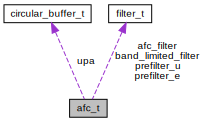
\includegraphics[width=275pt]{structafc__t__coll__graph}
\end{center}
\end{figure}
\subsection*{Data Fields}
\begin{DoxyCompactItemize}
\item 
\mbox{\hyperlink{filter_8h_a69e34b8aa259d2ca0b81b5c95f395bdf}{Filter}} \mbox{\hyperlink{structafc__t_a33db3fc1bf008116481e632f6080972c}{afc\+\_\+filter}}
\begin{DoxyCompactList}\small\item\em A\+FC filter W(z) \end{DoxyCompactList}\item 
\mbox{\hyperlink{filter_8h_a69e34b8aa259d2ca0b81b5c95f395bdf}{Filter}} \mbox{\hyperlink{structafc__t_a67b0483fc918fc9af5cb64c6b79e41cf}{prefilter\+\_\+e}}
\begin{DoxyCompactList}\small\item\em Pre-\/whitening filter A(z) \end{DoxyCompactList}\item 
\mbox{\hyperlink{filter_8h_a69e34b8aa259d2ca0b81b5c95f395bdf}{Filter}} \mbox{\hyperlink{structafc__t_a43d15e690ac1c74461c8b8a5522d8e52}{prefilter\+\_\+u}}
\begin{DoxyCompactList}\small\item\em Pre-\/whitening filter A(z) \end{DoxyCompactList}\item 
\mbox{\hyperlink{filter_8h_a69e34b8aa259d2ca0b81b5c95f395bdf}{Filter}} \mbox{\hyperlink{structafc__t_ad649e5413644e0dd06b2dfe789dd0630}{band\+\_\+limited\+\_\+filter}}
\begin{DoxyCompactList}\small\item\em Band-\/limited filter H(z) \end{DoxyCompactList}\item 
unsigned int \mbox{\hyperlink{structafc__t_ad09604e56d2183c494456350cbb709ea}{adaptation\+\_\+type}}
\item 
float $\ast$ \mbox{\hyperlink{structafc__t_aa69482203264d41b13f96cda153faec3}{u}}
\begin{DoxyCompactList}\small\item\em Band-\/limited signal u(n) of the HA output s(n) \end{DoxyCompactList}\item 
float $\ast$ \mbox{\hyperlink{structafc__t_a7c5db3530c08c1bec07d6f4bf921537d}{y\+\_\+hat}}
\begin{DoxyCompactList}\small\item\em Estimate of feedback signal y\+\_\+hat(n) \end{DoxyCompactList}\item 
float \mbox{\hyperlink{structafc__t_ab94a0e3f15733272ecd739279e132818}{power\+\_\+estimate}}
\begin{DoxyCompactList}\small\item\em Power estimate, sigma$^\wedge$2\+\_\+hat(n), of the input to coefficient adaptation bloclk. \end{DoxyCompactList}\item 
int \mbox{\hyperlink{structafc__t_acb59e5af368aca0b2840fa76e5e5a000}{frame\+\_\+size}}
\begin{DoxyCompactList}\small\item\em Number of samples in the current frame. \end{DoxyCompactList}\item 
float \mbox{\hyperlink{structafc__t_a7b343e47789c5a03ba4a37671c281861}{mu}}
\begin{DoxyCompactList}\small\item\em Step size parameter. \end{DoxyCompactList}\item 
float \mbox{\hyperlink{structafc__t_a472432ba992e61143df0a1ab83981c10}{delta}}
\begin{DoxyCompactList}\small\item\em Regularization term. \end{DoxyCompactList}\item 
float \mbox{\hyperlink{structafc__t_a8edae5604a2d189f1e83b71678566cad}{rho}}
\begin{DoxyCompactList}\small\item\em Forgetting factor. \end{DoxyCompactList}\item 
float \mbox{\hyperlink{structafc__t_a161775274c257b1d804c61b77cfbbbd7}{alpha}}
\begin{DoxyCompactList}\small\item\em Parameter for P\+N\+L\+MS. \end{DoxyCompactList}\item 
float \mbox{\hyperlink{structafc__t_a829042affbb45e80df502fc95134b673}{beta}}
\begin{DoxyCompactList}\small\item\em Parameter for P\+N\+L\+MS. \end{DoxyCompactList}\item 
float $\ast$ \mbox{\hyperlink{structafc__t_af7b50d899dcdfc8c68f6866764861f5f}{u\+\_\+prefiltered\+\_\+accumulated}}
\begin{DoxyCompactList}\small\item\em A\+F\+C\+\_\+\+N\+U\+M\+\_\+\+F\+R\+A\+M\+ES frames accumulated values of pre-\/filtered output of u(n). i.\+e. u\+\_\+f(n) \end{DoxyCompactList}\item 
\mbox{\hyperlink{circular__buffer_8h_aa88184dd60879f696cb2e679d0e50b45}{Circular\+\_\+buffer}} \mbox{\hyperlink{structafc__t_a11328ef1f3d92c69c404c5df7761116a}{upa}}
\end{DoxyCompactItemize}


\subsection{Detailed Description}
A\+FC data structure. 

Refer to the supported document on A\+FC for the notations 

\subsection{Field Documentation}
\mbox{\Hypertarget{structafc__t_ad09604e56d2183c494456350cbb709ea}\label{structafc__t_ad09604e56d2183c494456350cbb709ea}} 
\index{afc\+\_\+t@{afc\+\_\+t}!adaptation\+\_\+type@{adaptation\+\_\+type}}
\index{adaptation\+\_\+type@{adaptation\+\_\+type}!afc\+\_\+t@{afc\+\_\+t}}
\subsubsection{\texorpdfstring{adaptation\+\_\+type}{adaptation\_type}}
{\footnotesize\ttfamily unsigned int afc\+\_\+t\+::adaptation\+\_\+type}

\mbox{\Hypertarget{structafc__t_a33db3fc1bf008116481e632f6080972c}\label{structafc__t_a33db3fc1bf008116481e632f6080972c}} 
\index{afc\+\_\+t@{afc\+\_\+t}!afc\+\_\+filter@{afc\+\_\+filter}}
\index{afc\+\_\+filter@{afc\+\_\+filter}!afc\+\_\+t@{afc\+\_\+t}}
\subsubsection{\texorpdfstring{afc\+\_\+filter}{afc\_filter}}
{\footnotesize\ttfamily \mbox{\hyperlink{filter_8h_a69e34b8aa259d2ca0b81b5c95f395bdf}{Filter}} afc\+\_\+t\+::afc\+\_\+filter}



A\+FC filter W(z) 

\mbox{\Hypertarget{structafc__t_a161775274c257b1d804c61b77cfbbbd7}\label{structafc__t_a161775274c257b1d804c61b77cfbbbd7}} 
\index{afc\+\_\+t@{afc\+\_\+t}!alpha@{alpha}}
\index{alpha@{alpha}!afc\+\_\+t@{afc\+\_\+t}}
\subsubsection{\texorpdfstring{alpha}{alpha}}
{\footnotesize\ttfamily float afc\+\_\+t\+::alpha}



Parameter for P\+N\+L\+MS. 

\mbox{\Hypertarget{structafc__t_ad649e5413644e0dd06b2dfe789dd0630}\label{structafc__t_ad649e5413644e0dd06b2dfe789dd0630}} 
\index{afc\+\_\+t@{afc\+\_\+t}!band\+\_\+limited\+\_\+filter@{band\+\_\+limited\+\_\+filter}}
\index{band\+\_\+limited\+\_\+filter@{band\+\_\+limited\+\_\+filter}!afc\+\_\+t@{afc\+\_\+t}}
\subsubsection{\texorpdfstring{band\+\_\+limited\+\_\+filter}{band\_limited\_filter}}
{\footnotesize\ttfamily \mbox{\hyperlink{filter_8h_a69e34b8aa259d2ca0b81b5c95f395bdf}{Filter}} afc\+\_\+t\+::band\+\_\+limited\+\_\+filter}



Band-\/limited filter H(z) 

\mbox{\Hypertarget{structafc__t_a829042affbb45e80df502fc95134b673}\label{structafc__t_a829042affbb45e80df502fc95134b673}} 
\index{afc\+\_\+t@{afc\+\_\+t}!beta@{beta}}
\index{beta@{beta}!afc\+\_\+t@{afc\+\_\+t}}
\subsubsection{\texorpdfstring{beta}{beta}}
{\footnotesize\ttfamily float afc\+\_\+t\+::beta}



Parameter for P\+N\+L\+MS. 

\mbox{\Hypertarget{structafc__t_a472432ba992e61143df0a1ab83981c10}\label{structafc__t_a472432ba992e61143df0a1ab83981c10}} 
\index{afc\+\_\+t@{afc\+\_\+t}!delta@{delta}}
\index{delta@{delta}!afc\+\_\+t@{afc\+\_\+t}}
\subsubsection{\texorpdfstring{delta}{delta}}
{\footnotesize\ttfamily float afc\+\_\+t\+::delta}



Regularization term. 

\mbox{\Hypertarget{structafc__t_acb59e5af368aca0b2840fa76e5e5a000}\label{structafc__t_acb59e5af368aca0b2840fa76e5e5a000}} 
\index{afc\+\_\+t@{afc\+\_\+t}!frame\+\_\+size@{frame\+\_\+size}}
\index{frame\+\_\+size@{frame\+\_\+size}!afc\+\_\+t@{afc\+\_\+t}}
\subsubsection{\texorpdfstring{frame\+\_\+size}{frame\_size}}
{\footnotesize\ttfamily int afc\+\_\+t\+::frame\+\_\+size}



Number of samples in the current frame. 

\mbox{\Hypertarget{structafc__t_a7b343e47789c5a03ba4a37671c281861}\label{structafc__t_a7b343e47789c5a03ba4a37671c281861}} 
\index{afc\+\_\+t@{afc\+\_\+t}!mu@{mu}}
\index{mu@{mu}!afc\+\_\+t@{afc\+\_\+t}}
\subsubsection{\texorpdfstring{mu}{mu}}
{\footnotesize\ttfamily float afc\+\_\+t\+::mu}



Step size parameter. 

\mbox{\Hypertarget{structafc__t_ab94a0e3f15733272ecd739279e132818}\label{structafc__t_ab94a0e3f15733272ecd739279e132818}} 
\index{afc\+\_\+t@{afc\+\_\+t}!power\+\_\+estimate@{power\+\_\+estimate}}
\index{power\+\_\+estimate@{power\+\_\+estimate}!afc\+\_\+t@{afc\+\_\+t}}
\subsubsection{\texorpdfstring{power\+\_\+estimate}{power\_estimate}}
{\footnotesize\ttfamily float afc\+\_\+t\+::power\+\_\+estimate}



Power estimate, sigma$^\wedge$2\+\_\+hat(n), of the input to coefficient adaptation bloclk. 

\mbox{\Hypertarget{structafc__t_a67b0483fc918fc9af5cb64c6b79e41cf}\label{structafc__t_a67b0483fc918fc9af5cb64c6b79e41cf}} 
\index{afc\+\_\+t@{afc\+\_\+t}!prefilter\+\_\+e@{prefilter\+\_\+e}}
\index{prefilter\+\_\+e@{prefilter\+\_\+e}!afc\+\_\+t@{afc\+\_\+t}}
\subsubsection{\texorpdfstring{prefilter\+\_\+e}{prefilter\_e}}
{\footnotesize\ttfamily \mbox{\hyperlink{filter_8h_a69e34b8aa259d2ca0b81b5c95f395bdf}{Filter}} afc\+\_\+t\+::prefilter\+\_\+e}



Pre-\/whitening filter A(z) 

\mbox{\Hypertarget{structafc__t_a43d15e690ac1c74461c8b8a5522d8e52}\label{structafc__t_a43d15e690ac1c74461c8b8a5522d8e52}} 
\index{afc\+\_\+t@{afc\+\_\+t}!prefilter\+\_\+u@{prefilter\+\_\+u}}
\index{prefilter\+\_\+u@{prefilter\+\_\+u}!afc\+\_\+t@{afc\+\_\+t}}
\subsubsection{\texorpdfstring{prefilter\+\_\+u}{prefilter\_u}}
{\footnotesize\ttfamily \mbox{\hyperlink{filter_8h_a69e34b8aa259d2ca0b81b5c95f395bdf}{Filter}} afc\+\_\+t\+::prefilter\+\_\+u}



Pre-\/whitening filter A(z) 

\mbox{\Hypertarget{structafc__t_a8edae5604a2d189f1e83b71678566cad}\label{structafc__t_a8edae5604a2d189f1e83b71678566cad}} 
\index{afc\+\_\+t@{afc\+\_\+t}!rho@{rho}}
\index{rho@{rho}!afc\+\_\+t@{afc\+\_\+t}}
\subsubsection{\texorpdfstring{rho}{rho}}
{\footnotesize\ttfamily float afc\+\_\+t\+::rho}



Forgetting factor. 

\mbox{\Hypertarget{structafc__t_aa69482203264d41b13f96cda153faec3}\label{structafc__t_aa69482203264d41b13f96cda153faec3}} 
\index{afc\+\_\+t@{afc\+\_\+t}!u@{u}}
\index{u@{u}!afc\+\_\+t@{afc\+\_\+t}}
\subsubsection{\texorpdfstring{u}{u}}
{\footnotesize\ttfamily float$\ast$ afc\+\_\+t\+::u}



Band-\/limited signal u(n) of the HA output s(n) 

\mbox{\Hypertarget{structafc__t_af7b50d899dcdfc8c68f6866764861f5f}\label{structafc__t_af7b50d899dcdfc8c68f6866764861f5f}} 
\index{afc\+\_\+t@{afc\+\_\+t}!u\+\_\+prefiltered\+\_\+accumulated@{u\+\_\+prefiltered\+\_\+accumulated}}
\index{u\+\_\+prefiltered\+\_\+accumulated@{u\+\_\+prefiltered\+\_\+accumulated}!afc\+\_\+t@{afc\+\_\+t}}
\subsubsection{\texorpdfstring{u\+\_\+prefiltered\+\_\+accumulated}{u\_prefiltered\_accumulated}}
{\footnotesize\ttfamily float$\ast$ afc\+\_\+t\+::u\+\_\+prefiltered\+\_\+accumulated}



A\+F\+C\+\_\+\+N\+U\+M\+\_\+\+F\+R\+A\+M\+ES frames accumulated values of pre-\/filtered output of u(n). i.\+e. u\+\_\+f(n) 

\mbox{\Hypertarget{structafc__t_a11328ef1f3d92c69c404c5df7761116a}\label{structafc__t_a11328ef1f3d92c69c404c5df7761116a}} 
\index{afc\+\_\+t@{afc\+\_\+t}!upa@{upa}}
\index{upa@{upa}!afc\+\_\+t@{afc\+\_\+t}}
\subsubsection{\texorpdfstring{upa}{upa}}
{\footnotesize\ttfamily \mbox{\hyperlink{circular__buffer_8h_aa88184dd60879f696cb2e679d0e50b45}{Circular\+\_\+buffer}} afc\+\_\+t\+::upa}

\mbox{\Hypertarget{structafc__t_a7c5db3530c08c1bec07d6f4bf921537d}\label{structafc__t_a7c5db3530c08c1bec07d6f4bf921537d}} 
\index{afc\+\_\+t@{afc\+\_\+t}!y\+\_\+hat@{y\+\_\+hat}}
\index{y\+\_\+hat@{y\+\_\+hat}!afc\+\_\+t@{afc\+\_\+t}}
\subsubsection{\texorpdfstring{y\+\_\+hat}{y\_hat}}
{\footnotesize\ttfamily float$\ast$ afc\+\_\+t\+::y\+\_\+hat}



Estimate of feedback signal y\+\_\+hat(n) 



The documentation for this struct was generated from the following file\+:\begin{DoxyCompactItemize}
\item 
libosp/afc/\mbox{\hyperlink{afc_8c}{afc.\+c}}\end{DoxyCompactItemize}

\hypertarget{structbeam__form__t}{}\section{beam\+\_\+form\+\_\+t Struct Reference}
\label{structbeam__form__t}\index{beam\+\_\+form\+\_\+t@{beam\+\_\+form\+\_\+t}}


data structure containing relevant beam-\/forming fields  




Collaboration diagram for beam\+\_\+form\+\_\+t\+:\nopagebreak
\begin{figure}[H]
\begin{center}
\leavevmode
\includegraphics[width=165pt]{structbeam__form__t__coll__graph}
\end{center}
\end{figure}
\subsection*{Data Fields}
\begin{DoxyCompactItemize}
\item 
\mbox{\hyperlink{delay__line_8h_aa62b49f8bfee0c3a174896c9b446d68d}{Delay\+\_\+\+Line}} \mbox{\hyperlink{structbeam__form__t_ac6ce5ad03bc83781b2752c67b3803871}{delay\+\_\+line}}
\begin{DoxyCompactList}\small\item\em instance of delay\+\_\+line structure \end{DoxyCompactList}\item 
float \mbox{\hyperlink{structbeam__form__t_a327d18550d19abd047f7f89711ac61fc}{beta}}
\begin{DoxyCompactList}\small\item\em Rear microphone delay = beta $\ast$ D\+I\+S\+T\+A\+N\+CE / S\+P\+E\+E\+D\+\_\+\+O\+F\+\_\+\+S\+O\+U\+ND. \end{DoxyCompactList}\item 
float \mbox{\hyperlink{structbeam__form__t_a0fa1b33edfad76e13c1593da0537070e}{gain}}
\begin{DoxyCompactList}\small\item\em Rear microphone gain. \end{DoxyCompactList}\item 
unsigned char \mbox{\hyperlink{structbeam__form__t_a6358c3b8f9b4940a50c7fe48bade9e6b}{no\+\_\+delay}}
\begin{DoxyCompactList}\small\item\em Bypasses delay line code if there\textquotesingle{}s no delay Might remove. \end{DoxyCompactList}\end{DoxyCompactItemize}


\subsection{Detailed Description}
data structure containing relevant beam-\/forming fields 

\subsection{Field Documentation}
\mbox{\Hypertarget{structbeam__form__t_a327d18550d19abd047f7f89711ac61fc}\label{structbeam__form__t_a327d18550d19abd047f7f89711ac61fc}} 
\index{beam\+\_\+form\+\_\+t@{beam\+\_\+form\+\_\+t}!beta@{beta}}
\index{beta@{beta}!beam\+\_\+form\+\_\+t@{beam\+\_\+form\+\_\+t}}
\subsubsection{\texorpdfstring{beta}{beta}}
{\footnotesize\ttfamily float beam\+\_\+form\+\_\+t\+::beta}



Rear microphone delay = beta $\ast$ D\+I\+S\+T\+A\+N\+CE / S\+P\+E\+E\+D\+\_\+\+O\+F\+\_\+\+S\+O\+U\+ND. 

\mbox{\Hypertarget{structbeam__form__t_ac6ce5ad03bc83781b2752c67b3803871}\label{structbeam__form__t_ac6ce5ad03bc83781b2752c67b3803871}} 
\index{beam\+\_\+form\+\_\+t@{beam\+\_\+form\+\_\+t}!delay\+\_\+line@{delay\+\_\+line}}
\index{delay\+\_\+line@{delay\+\_\+line}!beam\+\_\+form\+\_\+t@{beam\+\_\+form\+\_\+t}}
\subsubsection{\texorpdfstring{delay\+\_\+line}{delay\_line}}
{\footnotesize\ttfamily \mbox{\hyperlink{delay__line_8h_aa62b49f8bfee0c3a174896c9b446d68d}{Delay\+\_\+\+Line}} beam\+\_\+form\+\_\+t\+::delay\+\_\+line}



instance of delay\+\_\+line structure 

\mbox{\Hypertarget{structbeam__form__t_a0fa1b33edfad76e13c1593da0537070e}\label{structbeam__form__t_a0fa1b33edfad76e13c1593da0537070e}} 
\index{beam\+\_\+form\+\_\+t@{beam\+\_\+form\+\_\+t}!gain@{gain}}
\index{gain@{gain}!beam\+\_\+form\+\_\+t@{beam\+\_\+form\+\_\+t}}
\subsubsection{\texorpdfstring{gain}{gain}}
{\footnotesize\ttfamily float beam\+\_\+form\+\_\+t\+::gain}



Rear microphone gain. 

\mbox{\Hypertarget{structbeam__form__t_a6358c3b8f9b4940a50c7fe48bade9e6b}\label{structbeam__form__t_a6358c3b8f9b4940a50c7fe48bade9e6b}} 
\index{beam\+\_\+form\+\_\+t@{beam\+\_\+form\+\_\+t}!no\+\_\+delay@{no\+\_\+delay}}
\index{no\+\_\+delay@{no\+\_\+delay}!beam\+\_\+form\+\_\+t@{beam\+\_\+form\+\_\+t}}
\subsubsection{\texorpdfstring{no\+\_\+delay}{no\_delay}}
{\footnotesize\ttfamily unsigned char beam\+\_\+form\+\_\+t\+::no\+\_\+delay}



Bypasses delay line code if there\textquotesingle{}s no delay Might remove. 



The documentation for this struct was generated from the following file\+:\begin{DoxyCompactItemize}
\item 
libosp/beam\+\_\+forming/\mbox{\hyperlink{beam__forming_8c}{beam\+\_\+forming.\+c}}\end{DoxyCompactItemize}

\hypertarget{structcircular__buffer__t}{}\section{circular\+\_\+buffer\+\_\+t Struct Reference}
\label{structcircular__buffer__t}\index{circular\+\_\+buffer\+\_\+t@{circular\+\_\+buffer\+\_\+t}}
\subsection*{Data Fields}
\begin{DoxyCompactItemize}
\item 
float $\ast$ \mbox{\hyperlink{structcircular__buffer__t_a05450b503674f101e5fa09fe2fe14d76}{buf}}
\item 
size\+\_\+t \mbox{\hyperlink{structcircular__buffer__t_ab00ef7eea313237690dfe2814951b9af}{length}}
\item 
size\+\_\+t \mbox{\hyperlink{structcircular__buffer__t_abf5dfce0f419464de0d19038065e88f5}{index}}
\item 
size\+\_\+t \mbox{\hyperlink{structcircular__buffer__t_a4eafcd801df588817b905950853704ff}{buf\+\_\+len}}
\item 
unsigned char \mbox{\hyperlink{structcircular__buffer__t_a6d2ad0faed1273fda0e34e0c4c1e010d}{exp}}
\end{DoxyCompactItemize}


\subsection{Field Documentation}
\mbox{\Hypertarget{structcircular__buffer__t_a05450b503674f101e5fa09fe2fe14d76}\label{structcircular__buffer__t_a05450b503674f101e5fa09fe2fe14d76}} 
\index{circular\+\_\+buffer\+\_\+t@{circular\+\_\+buffer\+\_\+t}!buf@{buf}}
\index{buf@{buf}!circular\+\_\+buffer\+\_\+t@{circular\+\_\+buffer\+\_\+t}}
\subsubsection{\texorpdfstring{buf}{buf}}
{\footnotesize\ttfamily float$\ast$ circular\+\_\+buffer\+\_\+t\+::buf}

\mbox{\Hypertarget{structcircular__buffer__t_a4eafcd801df588817b905950853704ff}\label{structcircular__buffer__t_a4eafcd801df588817b905950853704ff}} 
\index{circular\+\_\+buffer\+\_\+t@{circular\+\_\+buffer\+\_\+t}!buf\+\_\+len@{buf\+\_\+len}}
\index{buf\+\_\+len@{buf\+\_\+len}!circular\+\_\+buffer\+\_\+t@{circular\+\_\+buffer\+\_\+t}}
\subsubsection{\texorpdfstring{buf\+\_\+len}{buf\_len}}
{\footnotesize\ttfamily size\+\_\+t circular\+\_\+buffer\+\_\+t\+::buf\+\_\+len}

\mbox{\Hypertarget{structcircular__buffer__t_a6d2ad0faed1273fda0e34e0c4c1e010d}\label{structcircular__buffer__t_a6d2ad0faed1273fda0e34e0c4c1e010d}} 
\index{circular\+\_\+buffer\+\_\+t@{circular\+\_\+buffer\+\_\+t}!exp@{exp}}
\index{exp@{exp}!circular\+\_\+buffer\+\_\+t@{circular\+\_\+buffer\+\_\+t}}
\subsubsection{\texorpdfstring{exp}{exp}}
{\footnotesize\ttfamily unsigned char circular\+\_\+buffer\+\_\+t\+::exp}

\mbox{\Hypertarget{structcircular__buffer__t_abf5dfce0f419464de0d19038065e88f5}\label{structcircular__buffer__t_abf5dfce0f419464de0d19038065e88f5}} 
\index{circular\+\_\+buffer\+\_\+t@{circular\+\_\+buffer\+\_\+t}!index@{index}}
\index{index@{index}!circular\+\_\+buffer\+\_\+t@{circular\+\_\+buffer\+\_\+t}}
\subsubsection{\texorpdfstring{index}{index}}
{\footnotesize\ttfamily size\+\_\+t circular\+\_\+buffer\+\_\+t\+::index}

\mbox{\Hypertarget{structcircular__buffer__t_ab00ef7eea313237690dfe2814951b9af}\label{structcircular__buffer__t_ab00ef7eea313237690dfe2814951b9af}} 
\index{circular\+\_\+buffer\+\_\+t@{circular\+\_\+buffer\+\_\+t}!length@{length}}
\index{length@{length}!circular\+\_\+buffer\+\_\+t@{circular\+\_\+buffer\+\_\+t}}
\subsubsection{\texorpdfstring{length}{length}}
{\footnotesize\ttfamily size\+\_\+t circular\+\_\+buffer\+\_\+t\+::length}



The documentation for this struct was generated from the following file\+:\begin{DoxyCompactItemize}
\item 
libosp/afc/\mbox{\hyperlink{circular__buffer_8c}{circular\+\_\+buffer.\+c}}\end{DoxyCompactItemize}

\hypertarget{structdelay__line__t}{}\section{delay\+\_\+line\+\_\+t Struct Reference}
\label{structdelay__line__t}\index{delay\+\_\+line\+\_\+t@{delay\+\_\+line\+\_\+t}}


Data structure that contains delay\+\_\+line information.  


\subsection*{Data Fields}
\begin{DoxyCompactItemize}
\item 
float $\ast$ \mbox{\hyperlink{structdelay__line__t_ab306b10f6d4ba74e6283ff0f3f75d3de}{delay\+\_\+buffer}}
\begin{DoxyCompactList}\small\item\em The circ. buffer containing old delay\+\_\+line samples. \end{DoxyCompactList}\item 
long \mbox{\hyperlink{structdelay__line__t_a37c6b3ad5d2d500817bf4bb3eb2f6f8d}{delay\+\_\+size}}
\begin{DoxyCompactList}\small\item\em Size of the delay. Set up on init. \end{DoxyCompactList}\item 
long \mbox{\hyperlink{structdelay__line__t_adf31bf9bd65edf272a237fc3fe5da4a0}{delay\+\_\+mask}}
\item 
long \mbox{\hyperlink{structdelay__line__t_a703f4e6cacaf50647c3b82ebe5c9c349}{write\+\_\+pointer}}
\begin{DoxyCompactList}\small\item\em Write pointer of circular buffer. \end{DoxyCompactList}\end{DoxyCompactItemize}


\subsection{Detailed Description}
Data structure that contains delay\+\_\+line information. 

\subsection{Field Documentation}
\mbox{\Hypertarget{structdelay__line__t_ab306b10f6d4ba74e6283ff0f3f75d3de}\label{structdelay__line__t_ab306b10f6d4ba74e6283ff0f3f75d3de}} 
\index{delay\+\_\+line\+\_\+t@{delay\+\_\+line\+\_\+t}!delay\+\_\+buffer@{delay\+\_\+buffer}}
\index{delay\+\_\+buffer@{delay\+\_\+buffer}!delay\+\_\+line\+\_\+t@{delay\+\_\+line\+\_\+t}}
\subsubsection{\texorpdfstring{delay\+\_\+buffer}{delay\_buffer}}
{\footnotesize\ttfamily float$\ast$ delay\+\_\+line\+\_\+t\+::delay\+\_\+buffer}



The circ. buffer containing old delay\+\_\+line samples. 

\mbox{\Hypertarget{structdelay__line__t_adf31bf9bd65edf272a237fc3fe5da4a0}\label{structdelay__line__t_adf31bf9bd65edf272a237fc3fe5da4a0}} 
\index{delay\+\_\+line\+\_\+t@{delay\+\_\+line\+\_\+t}!delay\+\_\+mask@{delay\+\_\+mask}}
\index{delay\+\_\+mask@{delay\+\_\+mask}!delay\+\_\+line\+\_\+t@{delay\+\_\+line\+\_\+t}}
\subsubsection{\texorpdfstring{delay\+\_\+mask}{delay\_mask}}
{\footnotesize\ttfamily long delay\+\_\+line\+\_\+t\+::delay\+\_\+mask}

\mbox{\Hypertarget{structdelay__line__t_a37c6b3ad5d2d500817bf4bb3eb2f6f8d}\label{structdelay__line__t_a37c6b3ad5d2d500817bf4bb3eb2f6f8d}} 
\index{delay\+\_\+line\+\_\+t@{delay\+\_\+line\+\_\+t}!delay\+\_\+size@{delay\+\_\+size}}
\index{delay\+\_\+size@{delay\+\_\+size}!delay\+\_\+line\+\_\+t@{delay\+\_\+line\+\_\+t}}
\subsubsection{\texorpdfstring{delay\+\_\+size}{delay\_size}}
{\footnotesize\ttfamily long delay\+\_\+line\+\_\+t\+::delay\+\_\+size}



Size of the delay. Set up on init. 

\mbox{\Hypertarget{structdelay__line__t_a703f4e6cacaf50647c3b82ebe5c9c349}\label{structdelay__line__t_a703f4e6cacaf50647c3b82ebe5c9c349}} 
\index{delay\+\_\+line\+\_\+t@{delay\+\_\+line\+\_\+t}!write\+\_\+pointer@{write\+\_\+pointer}}
\index{write\+\_\+pointer@{write\+\_\+pointer}!delay\+\_\+line\+\_\+t@{delay\+\_\+line\+\_\+t}}
\subsubsection{\texorpdfstring{write\+\_\+pointer}{write\_pointer}}
{\footnotesize\ttfamily long delay\+\_\+line\+\_\+t\+::write\+\_\+pointer}



Write pointer of circular buffer. 



The documentation for this struct was generated from the following file\+:\begin{DoxyCompactItemize}
\item 
libosp/beam\+\_\+forming/\mbox{\hyperlink{delay__line_8c}{delay\+\_\+line.\+c}}\end{DoxyCompactItemize}

\hypertarget{structfile__loopback__context__t}{}\section{file\+\_\+loopback\+\_\+context\+\_\+t Struct Reference}
\label{structfile__loopback__context__t}\index{file\+\_\+loopback\+\_\+context\+\_\+t@{file\+\_\+loopback\+\_\+context\+\_\+t}}


Struct containing details for file loopback mode.  




{\ttfamily \#include $<$port\+\_\+wrapper.\+h$>$}

\subsection*{Data Fields}
\begin{DoxyCompactItemize}
\item 
F\+I\+LE $\ast$ \mbox{\hyperlink{structfile__loopback__context__t_a7af12b6f866e7f9b67ff5f28ee514581}{input\+\_\+file}}
\begin{DoxyCompactList}\small\item\em Input file. \end{DoxyCompactList}\item 
F\+I\+LE $\ast$ \mbox{\hyperlink{structfile__loopback__context__t_afc47a4ad1f9f0c3855101b48d96061a7}{output\+\_\+file}}
\begin{DoxyCompactList}\small\item\em Output file. \end{DoxyCompactList}\item 
unsigned long \mbox{\hyperlink{structfile__loopback__context__t_a444c3817f1985ad7acd3a94c32fccd90}{length}}
\begin{DoxyCompactList}\small\item\em Number of samples in input file. \end{DoxyCompactList}\item 
unsigned long \mbox{\hyperlink{structfile__loopback__context__t_a3510ddf92f42289c2997199a89eb9e23}{index}}
\begin{DoxyCompactList}\small\item\em Internal index var. \end{DoxyCompactList}\item 
char \mbox{\hyperlink{structfile__loopback__context__t_a87d194451bfb9775cb4ad94f6706f02b}{wav\+\_\+header}} \mbox{[}44\mbox{]}
\begin{DoxyCompactList}\small\item\em Header data embedded in .wav file. \end{DoxyCompactList}\item 
float $\ast$ \mbox{\hyperlink{structfile__loopback__context__t_a1b32087e30d7324c8069583b3390a919}{inL}}
\begin{DoxyCompactList}\small\item\em Array of input left samples. \end{DoxyCompactList}\item 
float $\ast$ \mbox{\hyperlink{structfile__loopback__context__t_aa62c08894838205cbfc5ebd2745bf88c}{inR}}
\begin{DoxyCompactList}\small\item\em Array of input right samples. \end{DoxyCompactList}\item 
float $\ast$ \mbox{\hyperlink{structfile__loopback__context__t_af2a4e77bb31f6b8cddf00af17c3e12f4}{outL}}
\begin{DoxyCompactList}\small\item\em Array of output left samples. \end{DoxyCompactList}\item 
float $\ast$ \mbox{\hyperlink{structfile__loopback__context__t_a91ec30b41cc5e8d834d5680f78ec80aa}{outR}}
\begin{DoxyCompactList}\small\item\em Array of output right samples. \end{DoxyCompactList}\end{DoxyCompactItemize}


\subsection{Detailed Description}
Struct containing details for file loopback mode. 

\subsection{Field Documentation}
\mbox{\Hypertarget{structfile__loopback__context__t_a3510ddf92f42289c2997199a89eb9e23}\label{structfile__loopback__context__t_a3510ddf92f42289c2997199a89eb9e23}} 
\index{file\+\_\+loopback\+\_\+context\+\_\+t@{file\+\_\+loopback\+\_\+context\+\_\+t}!index@{index}}
\index{index@{index}!file\+\_\+loopback\+\_\+context\+\_\+t@{file\+\_\+loopback\+\_\+context\+\_\+t}}
\subsubsection{\texorpdfstring{index}{index}}
{\footnotesize\ttfamily unsigned long file\+\_\+loopback\+\_\+context\+\_\+t\+::index}



Internal index var. 

\mbox{\Hypertarget{structfile__loopback__context__t_a1b32087e30d7324c8069583b3390a919}\label{structfile__loopback__context__t_a1b32087e30d7324c8069583b3390a919}} 
\index{file\+\_\+loopback\+\_\+context\+\_\+t@{file\+\_\+loopback\+\_\+context\+\_\+t}!inL@{inL}}
\index{inL@{inL}!file\+\_\+loopback\+\_\+context\+\_\+t@{file\+\_\+loopback\+\_\+context\+\_\+t}}
\subsubsection{\texorpdfstring{inL}{inL}}
{\footnotesize\ttfamily float$\ast$ file\+\_\+loopback\+\_\+context\+\_\+t\+::inL}



Array of input left samples. 

\mbox{\Hypertarget{structfile__loopback__context__t_a7af12b6f866e7f9b67ff5f28ee514581}\label{structfile__loopback__context__t_a7af12b6f866e7f9b67ff5f28ee514581}} 
\index{file\+\_\+loopback\+\_\+context\+\_\+t@{file\+\_\+loopback\+\_\+context\+\_\+t}!input\+\_\+file@{input\+\_\+file}}
\index{input\+\_\+file@{input\+\_\+file}!file\+\_\+loopback\+\_\+context\+\_\+t@{file\+\_\+loopback\+\_\+context\+\_\+t}}
\subsubsection{\texorpdfstring{input\+\_\+file}{input\_file}}
{\footnotesize\ttfamily F\+I\+LE$\ast$ file\+\_\+loopback\+\_\+context\+\_\+t\+::input\+\_\+file}



Input file. 

\mbox{\Hypertarget{structfile__loopback__context__t_aa62c08894838205cbfc5ebd2745bf88c}\label{structfile__loopback__context__t_aa62c08894838205cbfc5ebd2745bf88c}} 
\index{file\+\_\+loopback\+\_\+context\+\_\+t@{file\+\_\+loopback\+\_\+context\+\_\+t}!inR@{inR}}
\index{inR@{inR}!file\+\_\+loopback\+\_\+context\+\_\+t@{file\+\_\+loopback\+\_\+context\+\_\+t}}
\subsubsection{\texorpdfstring{inR}{inR}}
{\footnotesize\ttfamily float$\ast$ file\+\_\+loopback\+\_\+context\+\_\+t\+::inR}



Array of input right samples. 

\mbox{\Hypertarget{structfile__loopback__context__t_a444c3817f1985ad7acd3a94c32fccd90}\label{structfile__loopback__context__t_a444c3817f1985ad7acd3a94c32fccd90}} 
\index{file\+\_\+loopback\+\_\+context\+\_\+t@{file\+\_\+loopback\+\_\+context\+\_\+t}!length@{length}}
\index{length@{length}!file\+\_\+loopback\+\_\+context\+\_\+t@{file\+\_\+loopback\+\_\+context\+\_\+t}}
\subsubsection{\texorpdfstring{length}{length}}
{\footnotesize\ttfamily unsigned long file\+\_\+loopback\+\_\+context\+\_\+t\+::length}



Number of samples in input file. 

\mbox{\Hypertarget{structfile__loopback__context__t_af2a4e77bb31f6b8cddf00af17c3e12f4}\label{structfile__loopback__context__t_af2a4e77bb31f6b8cddf00af17c3e12f4}} 
\index{file\+\_\+loopback\+\_\+context\+\_\+t@{file\+\_\+loopback\+\_\+context\+\_\+t}!outL@{outL}}
\index{outL@{outL}!file\+\_\+loopback\+\_\+context\+\_\+t@{file\+\_\+loopback\+\_\+context\+\_\+t}}
\subsubsection{\texorpdfstring{outL}{outL}}
{\footnotesize\ttfamily float$\ast$ file\+\_\+loopback\+\_\+context\+\_\+t\+::outL}



Array of output left samples. 

\mbox{\Hypertarget{structfile__loopback__context__t_afc47a4ad1f9f0c3855101b48d96061a7}\label{structfile__loopback__context__t_afc47a4ad1f9f0c3855101b48d96061a7}} 
\index{file\+\_\+loopback\+\_\+context\+\_\+t@{file\+\_\+loopback\+\_\+context\+\_\+t}!output\+\_\+file@{output\+\_\+file}}
\index{output\+\_\+file@{output\+\_\+file}!file\+\_\+loopback\+\_\+context\+\_\+t@{file\+\_\+loopback\+\_\+context\+\_\+t}}
\subsubsection{\texorpdfstring{output\+\_\+file}{output\_file}}
{\footnotesize\ttfamily F\+I\+LE$\ast$ file\+\_\+loopback\+\_\+context\+\_\+t\+::output\+\_\+file}



Output file. 

\mbox{\Hypertarget{structfile__loopback__context__t_a91ec30b41cc5e8d834d5680f78ec80aa}\label{structfile__loopback__context__t_a91ec30b41cc5e8d834d5680f78ec80aa}} 
\index{file\+\_\+loopback\+\_\+context\+\_\+t@{file\+\_\+loopback\+\_\+context\+\_\+t}!outR@{outR}}
\index{outR@{outR}!file\+\_\+loopback\+\_\+context\+\_\+t@{file\+\_\+loopback\+\_\+context\+\_\+t}}
\subsubsection{\texorpdfstring{outR}{outR}}
{\footnotesize\ttfamily float$\ast$ file\+\_\+loopback\+\_\+context\+\_\+t\+::outR}



Array of output right samples. 

\mbox{\Hypertarget{structfile__loopback__context__t_a87d194451bfb9775cb4ad94f6706f02b}\label{structfile__loopback__context__t_a87d194451bfb9775cb4ad94f6706f02b}} 
\index{file\+\_\+loopback\+\_\+context\+\_\+t@{file\+\_\+loopback\+\_\+context\+\_\+t}!wav\+\_\+header@{wav\+\_\+header}}
\index{wav\+\_\+header@{wav\+\_\+header}!file\+\_\+loopback\+\_\+context\+\_\+t@{file\+\_\+loopback\+\_\+context\+\_\+t}}
\subsubsection{\texorpdfstring{wav\+\_\+header}{wav\_header}}
{\footnotesize\ttfamily char file\+\_\+loopback\+\_\+context\+\_\+t\+::wav\+\_\+header\mbox{[}44\mbox{]}}



Header data embedded in .wav file. 



The documentation for this struct was generated from the following file\+:\begin{DoxyCompactItemize}
\item 
osp/\mbox{\hyperlink{port__wrapper_8h}{port\+\_\+wrapper.\+h}}\end{DoxyCompactItemize}

\hypertarget{structfilter__t}{}\section{filter\+\_\+t Struct Reference}
\label{structfilter__t}\index{filter\+\_\+t@{filter\+\_\+t}}


Structure containing filter information.  


\subsection*{Data Fields}
\begin{DoxyCompactItemize}
\item 
float $\ast$ \mbox{\hyperlink{structfilter__t_a4d1dbe72019d23a1c4cb7621cfb5f7c7}{taps}}
\begin{DoxyCompactList}\small\item\em Taps of the filter (loaded in at init) \end{DoxyCompactList}\item 
float $\ast$ \mbox{\hyperlink{structfilter__t_a3567b5dd3dc06bcee781721b50565213}{buf}}
\begin{DoxyCompactList}\small\item\em Internal buffer. Keeps track of old samples between frames. \end{DoxyCompactList}\item 
int \mbox{\hyperlink{structfilter__t_a8b47a8b9661b7ebcad76afd55452b992}{length}}
\begin{DoxyCompactList}\small\item\em Length of the filter. \end{DoxyCompactList}\item 
int \mbox{\hyperlink{structfilter__t_a858cfd81f33da9ad7c085aec0bea5693}{index}}
\begin{DoxyCompactList}\small\item\em Internal index. Keeps track of where we are on internal buffer. \end{DoxyCompactList}\item 
unsigned int \mbox{\hyperlink{structfilter__t_a97a989230be5b2e10eecc3de6b2c7dbb}{buf\+\_\+len}}
\item 
unsigned char \mbox{\hyperlink{structfilter__t_acf95f97baf83ef8bb108d8c9e51a0d8b}{exp}}
\end{DoxyCompactItemize}


\subsection{Detailed Description}
Structure containing filter information. 

\subsection{Field Documentation}
\mbox{\Hypertarget{structfilter__t_a3567b5dd3dc06bcee781721b50565213}\label{structfilter__t_a3567b5dd3dc06bcee781721b50565213}} 
\index{filter\+\_\+t@{filter\+\_\+t}!buf@{buf}}
\index{buf@{buf}!filter\+\_\+t@{filter\+\_\+t}}
\subsubsection{\texorpdfstring{buf}{buf}}
{\footnotesize\ttfamily float$\ast$ filter\+\_\+t\+::buf}



Internal buffer. Keeps track of old samples between frames. 

\mbox{\Hypertarget{structfilter__t_a97a989230be5b2e10eecc3de6b2c7dbb}\label{structfilter__t_a97a989230be5b2e10eecc3de6b2c7dbb}} 
\index{filter\+\_\+t@{filter\+\_\+t}!buf\+\_\+len@{buf\+\_\+len}}
\index{buf\+\_\+len@{buf\+\_\+len}!filter\+\_\+t@{filter\+\_\+t}}
\subsubsection{\texorpdfstring{buf\+\_\+len}{buf\_len}}
{\footnotesize\ttfamily unsigned int filter\+\_\+t\+::buf\+\_\+len}

\mbox{\Hypertarget{structfilter__t_acf95f97baf83ef8bb108d8c9e51a0d8b}\label{structfilter__t_acf95f97baf83ef8bb108d8c9e51a0d8b}} 
\index{filter\+\_\+t@{filter\+\_\+t}!exp@{exp}}
\index{exp@{exp}!filter\+\_\+t@{filter\+\_\+t}}
\subsubsection{\texorpdfstring{exp}{exp}}
{\footnotesize\ttfamily unsigned char filter\+\_\+t\+::exp}

\mbox{\Hypertarget{structfilter__t_a858cfd81f33da9ad7c085aec0bea5693}\label{structfilter__t_a858cfd81f33da9ad7c085aec0bea5693}} 
\index{filter\+\_\+t@{filter\+\_\+t}!index@{index}}
\index{index@{index}!filter\+\_\+t@{filter\+\_\+t}}
\subsubsection{\texorpdfstring{index}{index}}
{\footnotesize\ttfamily int filter\+\_\+t\+::index}



Internal index. Keeps track of where we are on internal buffer. 

\mbox{\Hypertarget{structfilter__t_a8b47a8b9661b7ebcad76afd55452b992}\label{structfilter__t_a8b47a8b9661b7ebcad76afd55452b992}} 
\index{filter\+\_\+t@{filter\+\_\+t}!length@{length}}
\index{length@{length}!filter\+\_\+t@{filter\+\_\+t}}
\subsubsection{\texorpdfstring{length}{length}}
{\footnotesize\ttfamily int filter\+\_\+t\+::length}



Length of the filter. 

\mbox{\Hypertarget{structfilter__t_a4d1dbe72019d23a1c4cb7621cfb5f7c7}\label{structfilter__t_a4d1dbe72019d23a1c4cb7621cfb5f7c7}} 
\index{filter\+\_\+t@{filter\+\_\+t}!taps@{taps}}
\index{taps@{taps}!filter\+\_\+t@{filter\+\_\+t}}
\subsubsection{\texorpdfstring{taps}{taps}}
{\footnotesize\ttfamily float$\ast$ filter\+\_\+t\+::taps}



Taps of the filter (loaded in at init) 



The documentation for this struct was generated from the following file\+:\begin{DoxyCompactItemize}
\item 
libosp/filter/\mbox{\hyperlink{filter_8c}{filter.\+c}}\end{DoxyCompactItemize}

\hypertarget{structjsmn__parser}{}\section{jsmn\+\_\+parser Struct Reference}
\label{structjsmn__parser}\index{jsmn\+\_\+parser@{jsmn\+\_\+parser}}


{\ttfamily \#include $<$jsmn.\+h$>$}

\subsection*{Data Fields}
\begin{DoxyCompactItemize}
\item 
unsigned int \mbox{\hyperlink{structjsmn__parser_a3d0d6e48d3d5b24262f9e0c2241dc456}{pos}}
\item 
unsigned int \mbox{\hyperlink{structjsmn__parser_af640efd7d154218124a964b65f114bff}{toknext}}
\item 
int \mbox{\hyperlink{structjsmn__parser_af11fcec48d9f1298909777a12f1d1e39}{toksuper}}
\end{DoxyCompactItemize}


\subsection{Detailed Description}
J\+S\+ON parser. Contains an array of token blocks available. Also stores the string being parsed now and current position in that string 

\subsection{Field Documentation}
\mbox{\Hypertarget{structjsmn__parser_a3d0d6e48d3d5b24262f9e0c2241dc456}\label{structjsmn__parser_a3d0d6e48d3d5b24262f9e0c2241dc456}} 
\index{jsmn\+\_\+parser@{jsmn\+\_\+parser}!pos@{pos}}
\index{pos@{pos}!jsmn\+\_\+parser@{jsmn\+\_\+parser}}
\subsubsection{\texorpdfstring{pos}{pos}}
{\footnotesize\ttfamily unsigned int jsmn\+\_\+parser\+::pos}

\mbox{\Hypertarget{structjsmn__parser_af640efd7d154218124a964b65f114bff}\label{structjsmn__parser_af640efd7d154218124a964b65f114bff}} 
\index{jsmn\+\_\+parser@{jsmn\+\_\+parser}!toknext@{toknext}}
\index{toknext@{toknext}!jsmn\+\_\+parser@{jsmn\+\_\+parser}}
\subsubsection{\texorpdfstring{toknext}{toknext}}
{\footnotesize\ttfamily unsigned int jsmn\+\_\+parser\+::toknext}

\mbox{\Hypertarget{structjsmn__parser_af11fcec48d9f1298909777a12f1d1e39}\label{structjsmn__parser_af11fcec48d9f1298909777a12f1d1e39}} 
\index{jsmn\+\_\+parser@{jsmn\+\_\+parser}!toksuper@{toksuper}}
\index{toksuper@{toksuper}!jsmn\+\_\+parser@{jsmn\+\_\+parser}}
\subsubsection{\texorpdfstring{toksuper}{toksuper}}
{\footnotesize\ttfamily int jsmn\+\_\+parser\+::toksuper}



The documentation for this struct was generated from the following file\+:\begin{DoxyCompactItemize}
\item 
libosp/osp\+\_\+tcp/json\+\_\+parser/\mbox{\hyperlink{jsmn_8h}{jsmn.\+h}}\end{DoxyCompactItemize}

\hypertarget{structjsmntok__t}{}\section{jsmntok\+\_\+t Struct Reference}
\label{structjsmntok__t}\index{jsmntok\+\_\+t@{jsmntok\+\_\+t}}


{\ttfamily \#include $<$jsmn.\+h$>$}

\subsection*{Data Fields}
\begin{DoxyCompactItemize}
\item 
\mbox{\hyperlink{jsmn_8h_a065320719769f9dc1fbe30094e52802f}{jsmntype\+\_\+t}} \mbox{\hyperlink{structjsmntok__t_ac03dbd6b83cbcd979eb64702d5b9943e}{type}}
\item 
int \mbox{\hyperlink{structjsmntok__t_a0a8f55d0095f268ce8e224fe1234acd0}{start}}
\item 
int \mbox{\hyperlink{structjsmntok__t_ab49e0369f39e9b6174141e7f5bde5996}{end}}
\item 
int \mbox{\hyperlink{structjsmntok__t_a8ac3694b7335456c8e602197778883db}{size}}
\end{DoxyCompactItemize}


\subsection{Detailed Description}
J\+S\+ON token description. type type (object, array, string etc.) start start position in J\+S\+ON data string end end position in J\+S\+ON data string 

\subsection{Field Documentation}
\mbox{\Hypertarget{structjsmntok__t_ab49e0369f39e9b6174141e7f5bde5996}\label{structjsmntok__t_ab49e0369f39e9b6174141e7f5bde5996}} 
\index{jsmntok\+\_\+t@{jsmntok\+\_\+t}!end@{end}}
\index{end@{end}!jsmntok\+\_\+t@{jsmntok\+\_\+t}}
\subsubsection{\texorpdfstring{end}{end}}
{\footnotesize\ttfamily int jsmntok\+\_\+t\+::end}

\mbox{\Hypertarget{structjsmntok__t_a8ac3694b7335456c8e602197778883db}\label{structjsmntok__t_a8ac3694b7335456c8e602197778883db}} 
\index{jsmntok\+\_\+t@{jsmntok\+\_\+t}!size@{size}}
\index{size@{size}!jsmntok\+\_\+t@{jsmntok\+\_\+t}}
\subsubsection{\texorpdfstring{size}{size}}
{\footnotesize\ttfamily int jsmntok\+\_\+t\+::size}

\mbox{\Hypertarget{structjsmntok__t_a0a8f55d0095f268ce8e224fe1234acd0}\label{structjsmntok__t_a0a8f55d0095f268ce8e224fe1234acd0}} 
\index{jsmntok\+\_\+t@{jsmntok\+\_\+t}!start@{start}}
\index{start@{start}!jsmntok\+\_\+t@{jsmntok\+\_\+t}}
\subsubsection{\texorpdfstring{start}{start}}
{\footnotesize\ttfamily int jsmntok\+\_\+t\+::start}

\mbox{\Hypertarget{structjsmntok__t_ac03dbd6b83cbcd979eb64702d5b9943e}\label{structjsmntok__t_ac03dbd6b83cbcd979eb64702d5b9943e}} 
\index{jsmntok\+\_\+t@{jsmntok\+\_\+t}!type@{type}}
\index{type@{type}!jsmntok\+\_\+t@{jsmntok\+\_\+t}}
\subsubsection{\texorpdfstring{type}{type}}
{\footnotesize\ttfamily \mbox{\hyperlink{jsmn_8h_a065320719769f9dc1fbe30094e52802f}{jsmntype\+\_\+t}} jsmntok\+\_\+t\+::type}



The documentation for this struct was generated from the following file\+:\begin{DoxyCompactItemize}
\item 
libosp/osp\+\_\+tcp/json\+\_\+parser/\mbox{\hyperlink{jsmn_8h}{jsmn.\+h}}\end{DoxyCompactItemize}

\hypertarget{structosp__tcp__t}{}\section{osp\+\_\+tcp\+\_\+t Struct Reference}
\label{structosp__tcp__t}\index{osp\+\_\+tcp\+\_\+t@{osp\+\_\+tcp\+\_\+t}}


Data structure containing O\+SP T\+CP layer internal variables.  


\subsection*{Data Fields}
\begin{DoxyCompactItemize}
\item 
int \mbox{\hyperlink{structosp__tcp__t_afbf6dc5faef099a1e5a81e23d84290e7}{conn\+\_\+fd}}
\begin{DoxyCompactList}\small\item\em The socket file descriptor. \end{DoxyCompactList}\item 
int \mbox{\hyperlink{structosp__tcp__t_a944dbf95de27ec773bf9b4e169a30661}{sock}}
\begin{DoxyCompactList}\small\item\em The socket in to establish a connection. \end{DoxyCompactList}\item 
int \mbox{\hyperlink{structosp__tcp__t_a2b2fad6184d1ce632032645f85469657}{port}}
\begin{DoxyCompactList}\small\item\em The port to listen on for a connection. \end{DoxyCompactList}\end{DoxyCompactItemize}


\subsection{Detailed Description}
Data structure containing O\+SP T\+CP layer internal variables. 

\subsection{Field Documentation}
\mbox{\Hypertarget{structosp__tcp__t_afbf6dc5faef099a1e5a81e23d84290e7}\label{structosp__tcp__t_afbf6dc5faef099a1e5a81e23d84290e7}} 
\index{osp\+\_\+tcp\+\_\+t@{osp\+\_\+tcp\+\_\+t}!conn\+\_\+fd@{conn\+\_\+fd}}
\index{conn\+\_\+fd@{conn\+\_\+fd}!osp\+\_\+tcp\+\_\+t@{osp\+\_\+tcp\+\_\+t}}
\subsubsection{\texorpdfstring{conn\+\_\+fd}{conn\_fd}}
{\footnotesize\ttfamily int osp\+\_\+tcp\+\_\+t\+::conn\+\_\+fd}



The socket file descriptor. 

\mbox{\Hypertarget{structosp__tcp__t_a2b2fad6184d1ce632032645f85469657}\label{structosp__tcp__t_a2b2fad6184d1ce632032645f85469657}} 
\index{osp\+\_\+tcp\+\_\+t@{osp\+\_\+tcp\+\_\+t}!port@{port}}
\index{port@{port}!osp\+\_\+tcp\+\_\+t@{osp\+\_\+tcp\+\_\+t}}
\subsubsection{\texorpdfstring{port}{port}}
{\footnotesize\ttfamily int osp\+\_\+tcp\+\_\+t\+::port}



The port to listen on for a connection. 

\mbox{\Hypertarget{structosp__tcp__t_a944dbf95de27ec773bf9b4e169a30661}\label{structosp__tcp__t_a944dbf95de27ec773bf9b4e169a30661}} 
\index{osp\+\_\+tcp\+\_\+t@{osp\+\_\+tcp\+\_\+t}!sock@{sock}}
\index{sock@{sock}!osp\+\_\+tcp\+\_\+t@{osp\+\_\+tcp\+\_\+t}}
\subsubsection{\texorpdfstring{sock}{sock}}
{\footnotesize\ttfamily int osp\+\_\+tcp\+\_\+t\+::sock}



The socket in to establish a connection. 



The documentation for this struct was generated from the following file\+:\begin{DoxyCompactItemize}
\item 
libosp/osp\+\_\+tcp/\mbox{\hyperlink{osp__tcp_8c}{osp\+\_\+tcp.\+c}}\end{DoxyCompactItemize}

\hypertarget{structosp__user__data__t}{}\section{osp\+\_\+user\+\_\+data\+\_\+t Struct Reference}
\label{structosp__user__data__t}\index{osp\+\_\+user\+\_\+data\+\_\+t@{osp\+\_\+user\+\_\+data\+\_\+t}}


general data structure shared between client and C application  




{\ttfamily \#include $<$constants.\+h$>$}

\subsection*{Data Fields}
\begin{DoxyCompactItemize}
\item 
int \mbox{\hyperlink{structosp__user__data__t_ab6aa759f78ee1e7411c6591c88977c14}{no\+\_\+op}}
\begin{DoxyCompactList}\small\item\em No operation. The audio is passed from input to output in the audio callback. \end{DoxyCompactList}\item 
int \mbox{\hyperlink{structosp__user__data__t_a5eca0400f27a8aaf1b9ce3e961720af8}{afc}}
\begin{DoxyCompactList}\small\item\em A\+FC on/off. \end{DoxyCompactList}\item 
int \mbox{\hyperlink{structosp__user__data__t_a03a42dd2eac876e9bcea79061343d3df}{feedback}}
\begin{DoxyCompactList}\small\item\em Feedback on/off. \end{DoxyCompactList}\item 
int \mbox{\hyperlink{structosp__user__data__t_a509aa26b645cbc3436c862f0865f66a6}{rear\+\_\+mics}}
\begin{DoxyCompactList}\small\item\em Read mics on/off. \end{DoxyCompactList}\item 
int \mbox{\hyperlink{structosp__user__data__t_ae2f043926e510f9f990480346e2ba6fe}{g50}} \mbox{[}\mbox{\hyperlink{constants_8h_a19441d7b9be72492ed93a440085e53be}{N\+U\+M\+\_\+\+B\+A\+N\+DS}}\mbox{]}
\begin{DoxyCompactList}\small\item\em The gain values at 50 dB S\+PL input level. \end{DoxyCompactList}\item 
int \mbox{\hyperlink{structosp__user__data__t_a02d70968d64180808d46e4f76e066382}{g80}} \mbox{[}\mbox{\hyperlink{constants_8h_a19441d7b9be72492ed93a440085e53be}{N\+U\+M\+\_\+\+B\+A\+N\+DS}}\mbox{]}
\begin{DoxyCompactList}\small\item\em The gain values at 80 dB S\+PL input level. \end{DoxyCompactList}\item 
int \mbox{\hyperlink{structosp__user__data__t_a8709446147e7d44c5b9cfabe9e51799e}{knee\+\_\+low}} \mbox{[}\mbox{\hyperlink{constants_8h_a19441d7b9be72492ed93a440085e53be}{N\+U\+M\+\_\+\+B\+A\+N\+DS}}\mbox{]}
\begin{DoxyCompactList}\small\item\em Lower kneepoints for all bands. \end{DoxyCompactList}\item 
int \mbox{\hyperlink{structosp__user__data__t_a2564a1c5458026ce4a1532458886f5ab}{knee\+\_\+high}} \mbox{[}\mbox{\hyperlink{constants_8h_a19441d7b9be72492ed93a440085e53be}{N\+U\+M\+\_\+\+B\+A\+N\+DS}}\mbox{]}
\begin{DoxyCompactList}\small\item\em Upper kneepoints for all bands. \end{DoxyCompactList}\item 
int \mbox{\hyperlink{structosp__user__data__t_abb30fbb6fa960d660b72e18ecd82ee88}{attack}} \mbox{[}\mbox{\hyperlink{constants_8h_a19441d7b9be72492ed93a440085e53be}{N\+U\+M\+\_\+\+B\+A\+N\+DS}}\mbox{]}
\begin{DoxyCompactList}\small\item\em Attack time for W\+D\+RC for all bands. \end{DoxyCompactList}\item 
int \mbox{\hyperlink{structosp__user__data__t_ab1e8e99c42b77ee9f8920b678d94a1a5}{release}} \mbox{[}\mbox{\hyperlink{constants_8h_a19441d7b9be72492ed93a440085e53be}{N\+U\+M\+\_\+\+B\+A\+N\+DS}}\mbox{]}
\begin{DoxyCompactList}\small\item\em Release time for W\+D\+RC for all bands. \end{DoxyCompactList}\item 
int \mbox{\hyperlink{structosp__user__data__t_af265bd9d66e58eec5ac0b43a2f8e02cc}{mpo\+\_\+on}}
\begin{DoxyCompactList}\small\item\em toggle for M\+PO on/off \end{DoxyCompactList}\item 
int \mbox{\hyperlink{structosp__user__data__t_a7aac3aa1476589a9014fef82cbcc4c4c}{choose\+\_\+sampling\+\_\+frequency}}
\item 
int \mbox{\hyperlink{structosp__user__data__t_ab6c6864ef4a835caedfac8f7757d3646}{noise\+\_\+estimation\+\_\+type}}
\begin{DoxyCompactList}\small\item\em Choose type of Noise estimation technique. \end{DoxyCompactList}\item 
int \mbox{\hyperlink{structosp__user__data__t_a4d4b5738a5abe27d67dbbc278959defa}{spectral\+\_\+subtraction}}
\begin{DoxyCompactList}\small\item\em Spectral subtraction O\+N/\+O\+FF. \end{DoxyCompactList}\item 
float \mbox{\hyperlink{structosp__user__data__t_a21ab3e8e57f137d0308868f84d09631f}{spectral\+\_\+subtraction\+\_\+param}}
\begin{DoxyCompactList}\small\item\em Spectral subtraction parameter. \end{DoxyCompactList}\end{DoxyCompactItemize}


\subsection{Detailed Description}
general data structure shared between client and C application 

\subsection{Field Documentation}
\mbox{\Hypertarget{structosp__user__data__t_a5eca0400f27a8aaf1b9ce3e961720af8}\label{structosp__user__data__t_a5eca0400f27a8aaf1b9ce3e961720af8}} 
\index{osp\+\_\+user\+\_\+data\+\_\+t@{osp\+\_\+user\+\_\+data\+\_\+t}!afc@{afc}}
\index{afc@{afc}!osp\+\_\+user\+\_\+data\+\_\+t@{osp\+\_\+user\+\_\+data\+\_\+t}}
\subsubsection{\texorpdfstring{afc}{afc}}
{\footnotesize\ttfamily int osp\+\_\+user\+\_\+data\+\_\+t\+::afc}



A\+FC on/off. 

\mbox{\Hypertarget{structosp__user__data__t_abb30fbb6fa960d660b72e18ecd82ee88}\label{structosp__user__data__t_abb30fbb6fa960d660b72e18ecd82ee88}} 
\index{osp\+\_\+user\+\_\+data\+\_\+t@{osp\+\_\+user\+\_\+data\+\_\+t}!attack@{attack}}
\index{attack@{attack}!osp\+\_\+user\+\_\+data\+\_\+t@{osp\+\_\+user\+\_\+data\+\_\+t}}
\subsubsection{\texorpdfstring{attack}{attack}}
{\footnotesize\ttfamily int osp\+\_\+user\+\_\+data\+\_\+t\+::attack\mbox{[}\mbox{\hyperlink{constants_8h_a19441d7b9be72492ed93a440085e53be}{N\+U\+M\+\_\+\+B\+A\+N\+DS}}\mbox{]}}



Attack time for W\+D\+RC for all bands. 

\mbox{\Hypertarget{structosp__user__data__t_a7aac3aa1476589a9014fef82cbcc4c4c}\label{structosp__user__data__t_a7aac3aa1476589a9014fef82cbcc4c4c}} 
\index{osp\+\_\+user\+\_\+data\+\_\+t@{osp\+\_\+user\+\_\+data\+\_\+t}!choose\+\_\+sampling\+\_\+frequency@{choose\+\_\+sampling\+\_\+frequency}}
\index{choose\+\_\+sampling\+\_\+frequency@{choose\+\_\+sampling\+\_\+frequency}!osp\+\_\+user\+\_\+data\+\_\+t@{osp\+\_\+user\+\_\+data\+\_\+t}}
\subsubsection{\texorpdfstring{choose\+\_\+sampling\+\_\+frequency}{choose\_sampling\_frequency}}
{\footnotesize\ttfamily int osp\+\_\+user\+\_\+data\+\_\+t\+::choose\+\_\+sampling\+\_\+frequency}

\mbox{\Hypertarget{structosp__user__data__t_a03a42dd2eac876e9bcea79061343d3df}\label{structosp__user__data__t_a03a42dd2eac876e9bcea79061343d3df}} 
\index{osp\+\_\+user\+\_\+data\+\_\+t@{osp\+\_\+user\+\_\+data\+\_\+t}!feedback@{feedback}}
\index{feedback@{feedback}!osp\+\_\+user\+\_\+data\+\_\+t@{osp\+\_\+user\+\_\+data\+\_\+t}}
\subsubsection{\texorpdfstring{feedback}{feedback}}
{\footnotesize\ttfamily int osp\+\_\+user\+\_\+data\+\_\+t\+::feedback}



Feedback on/off. 

\mbox{\Hypertarget{structosp__user__data__t_ae2f043926e510f9f990480346e2ba6fe}\label{structosp__user__data__t_ae2f043926e510f9f990480346e2ba6fe}} 
\index{osp\+\_\+user\+\_\+data\+\_\+t@{osp\+\_\+user\+\_\+data\+\_\+t}!g50@{g50}}
\index{g50@{g50}!osp\+\_\+user\+\_\+data\+\_\+t@{osp\+\_\+user\+\_\+data\+\_\+t}}
\subsubsection{\texorpdfstring{g50}{g50}}
{\footnotesize\ttfamily int osp\+\_\+user\+\_\+data\+\_\+t\+::g50\mbox{[}\mbox{\hyperlink{constants_8h_a19441d7b9be72492ed93a440085e53be}{N\+U\+M\+\_\+\+B\+A\+N\+DS}}\mbox{]}}



The gain values at 50 dB S\+PL input level. 

\mbox{\Hypertarget{structosp__user__data__t_a02d70968d64180808d46e4f76e066382}\label{structosp__user__data__t_a02d70968d64180808d46e4f76e066382}} 
\index{osp\+\_\+user\+\_\+data\+\_\+t@{osp\+\_\+user\+\_\+data\+\_\+t}!g80@{g80}}
\index{g80@{g80}!osp\+\_\+user\+\_\+data\+\_\+t@{osp\+\_\+user\+\_\+data\+\_\+t}}
\subsubsection{\texorpdfstring{g80}{g80}}
{\footnotesize\ttfamily int osp\+\_\+user\+\_\+data\+\_\+t\+::g80\mbox{[}\mbox{\hyperlink{constants_8h_a19441d7b9be72492ed93a440085e53be}{N\+U\+M\+\_\+\+B\+A\+N\+DS}}\mbox{]}}



The gain values at 80 dB S\+PL input level. 

\mbox{\Hypertarget{structosp__user__data__t_a2564a1c5458026ce4a1532458886f5ab}\label{structosp__user__data__t_a2564a1c5458026ce4a1532458886f5ab}} 
\index{osp\+\_\+user\+\_\+data\+\_\+t@{osp\+\_\+user\+\_\+data\+\_\+t}!knee\+\_\+high@{knee\+\_\+high}}
\index{knee\+\_\+high@{knee\+\_\+high}!osp\+\_\+user\+\_\+data\+\_\+t@{osp\+\_\+user\+\_\+data\+\_\+t}}
\subsubsection{\texorpdfstring{knee\+\_\+high}{knee\_high}}
{\footnotesize\ttfamily int osp\+\_\+user\+\_\+data\+\_\+t\+::knee\+\_\+high\mbox{[}\mbox{\hyperlink{constants_8h_a19441d7b9be72492ed93a440085e53be}{N\+U\+M\+\_\+\+B\+A\+N\+DS}}\mbox{]}}



Upper kneepoints for all bands. 

\mbox{\Hypertarget{structosp__user__data__t_a8709446147e7d44c5b9cfabe9e51799e}\label{structosp__user__data__t_a8709446147e7d44c5b9cfabe9e51799e}} 
\index{osp\+\_\+user\+\_\+data\+\_\+t@{osp\+\_\+user\+\_\+data\+\_\+t}!knee\+\_\+low@{knee\+\_\+low}}
\index{knee\+\_\+low@{knee\+\_\+low}!osp\+\_\+user\+\_\+data\+\_\+t@{osp\+\_\+user\+\_\+data\+\_\+t}}
\subsubsection{\texorpdfstring{knee\+\_\+low}{knee\_low}}
{\footnotesize\ttfamily int osp\+\_\+user\+\_\+data\+\_\+t\+::knee\+\_\+low\mbox{[}\mbox{\hyperlink{constants_8h_a19441d7b9be72492ed93a440085e53be}{N\+U\+M\+\_\+\+B\+A\+N\+DS}}\mbox{]}}



Lower kneepoints for all bands. 

\mbox{\Hypertarget{structosp__user__data__t_af265bd9d66e58eec5ac0b43a2f8e02cc}\label{structosp__user__data__t_af265bd9d66e58eec5ac0b43a2f8e02cc}} 
\index{osp\+\_\+user\+\_\+data\+\_\+t@{osp\+\_\+user\+\_\+data\+\_\+t}!mpo\+\_\+on@{mpo\+\_\+on}}
\index{mpo\+\_\+on@{mpo\+\_\+on}!osp\+\_\+user\+\_\+data\+\_\+t@{osp\+\_\+user\+\_\+data\+\_\+t}}
\subsubsection{\texorpdfstring{mpo\+\_\+on}{mpo\_on}}
{\footnotesize\ttfamily int osp\+\_\+user\+\_\+data\+\_\+t\+::mpo\+\_\+on}



toggle for M\+PO on/off 

\mbox{\Hypertarget{structosp__user__data__t_ab6aa759f78ee1e7411c6591c88977c14}\label{structosp__user__data__t_ab6aa759f78ee1e7411c6591c88977c14}} 
\index{osp\+\_\+user\+\_\+data\+\_\+t@{osp\+\_\+user\+\_\+data\+\_\+t}!no\+\_\+op@{no\+\_\+op}}
\index{no\+\_\+op@{no\+\_\+op}!osp\+\_\+user\+\_\+data\+\_\+t@{osp\+\_\+user\+\_\+data\+\_\+t}}
\subsubsection{\texorpdfstring{no\+\_\+op}{no\_op}}
{\footnotesize\ttfamily int osp\+\_\+user\+\_\+data\+\_\+t\+::no\+\_\+op}



No operation. The audio is passed from input to output in the audio callback. 

\mbox{\Hypertarget{structosp__user__data__t_ab6c6864ef4a835caedfac8f7757d3646}\label{structosp__user__data__t_ab6c6864ef4a835caedfac8f7757d3646}} 
\index{osp\+\_\+user\+\_\+data\+\_\+t@{osp\+\_\+user\+\_\+data\+\_\+t}!noise\+\_\+estimation\+\_\+type@{noise\+\_\+estimation\+\_\+type}}
\index{noise\+\_\+estimation\+\_\+type@{noise\+\_\+estimation\+\_\+type}!osp\+\_\+user\+\_\+data\+\_\+t@{osp\+\_\+user\+\_\+data\+\_\+t}}
\subsubsection{\texorpdfstring{noise\+\_\+estimation\+\_\+type}{noise\_estimation\_type}}
{\footnotesize\ttfamily int osp\+\_\+user\+\_\+data\+\_\+t\+::noise\+\_\+estimation\+\_\+type}



Choose type of Noise estimation technique. 

\mbox{\Hypertarget{structosp__user__data__t_a509aa26b645cbc3436c862f0865f66a6}\label{structosp__user__data__t_a509aa26b645cbc3436c862f0865f66a6}} 
\index{osp\+\_\+user\+\_\+data\+\_\+t@{osp\+\_\+user\+\_\+data\+\_\+t}!rear\+\_\+mics@{rear\+\_\+mics}}
\index{rear\+\_\+mics@{rear\+\_\+mics}!osp\+\_\+user\+\_\+data\+\_\+t@{osp\+\_\+user\+\_\+data\+\_\+t}}
\subsubsection{\texorpdfstring{rear\+\_\+mics}{rear\_mics}}
{\footnotesize\ttfamily int osp\+\_\+user\+\_\+data\+\_\+t\+::rear\+\_\+mics}



Read mics on/off. 

\mbox{\Hypertarget{structosp__user__data__t_ab1e8e99c42b77ee9f8920b678d94a1a5}\label{structosp__user__data__t_ab1e8e99c42b77ee9f8920b678d94a1a5}} 
\index{osp\+\_\+user\+\_\+data\+\_\+t@{osp\+\_\+user\+\_\+data\+\_\+t}!release@{release}}
\index{release@{release}!osp\+\_\+user\+\_\+data\+\_\+t@{osp\+\_\+user\+\_\+data\+\_\+t}}
\subsubsection{\texorpdfstring{release}{release}}
{\footnotesize\ttfamily int osp\+\_\+user\+\_\+data\+\_\+t\+::release\mbox{[}\mbox{\hyperlink{constants_8h_a19441d7b9be72492ed93a440085e53be}{N\+U\+M\+\_\+\+B\+A\+N\+DS}}\mbox{]}}



Release time for W\+D\+RC for all bands. 

\mbox{\Hypertarget{structosp__user__data__t_a4d4b5738a5abe27d67dbbc278959defa}\label{structosp__user__data__t_a4d4b5738a5abe27d67dbbc278959defa}} 
\index{osp\+\_\+user\+\_\+data\+\_\+t@{osp\+\_\+user\+\_\+data\+\_\+t}!spectral\+\_\+subtraction@{spectral\+\_\+subtraction}}
\index{spectral\+\_\+subtraction@{spectral\+\_\+subtraction}!osp\+\_\+user\+\_\+data\+\_\+t@{osp\+\_\+user\+\_\+data\+\_\+t}}
\subsubsection{\texorpdfstring{spectral\+\_\+subtraction}{spectral\_subtraction}}
{\footnotesize\ttfamily int osp\+\_\+user\+\_\+data\+\_\+t\+::spectral\+\_\+subtraction}



Spectral subtraction O\+N/\+O\+FF. 

\mbox{\Hypertarget{structosp__user__data__t_a21ab3e8e57f137d0308868f84d09631f}\label{structosp__user__data__t_a21ab3e8e57f137d0308868f84d09631f}} 
\index{osp\+\_\+user\+\_\+data\+\_\+t@{osp\+\_\+user\+\_\+data\+\_\+t}!spectral\+\_\+subtraction\+\_\+param@{spectral\+\_\+subtraction\+\_\+param}}
\index{spectral\+\_\+subtraction\+\_\+param@{spectral\+\_\+subtraction\+\_\+param}!osp\+\_\+user\+\_\+data\+\_\+t@{osp\+\_\+user\+\_\+data\+\_\+t}}
\subsubsection{\texorpdfstring{spectral\+\_\+subtraction\+\_\+param}{spectral\_subtraction\_param}}
{\footnotesize\ttfamily float osp\+\_\+user\+\_\+data\+\_\+t\+::spectral\+\_\+subtraction\+\_\+param}



Spectral subtraction parameter. 



The documentation for this struct was generated from the following file\+:\begin{DoxyCompactItemize}
\item 
libosp/common/\mbox{\hyperlink{constants_8h}{constants.\+h}}\end{DoxyCompactItemize}

\hypertarget{structpa__aux__data__t}{}\section{pa\+\_\+aux\+\_\+data\+\_\+t Struct Reference}
\label{structpa__aux__data__t}\index{pa\+\_\+aux\+\_\+data\+\_\+t@{pa\+\_\+aux\+\_\+data\+\_\+t}}


Struct that contains misc data passed to Port\+Audio.  




{\ttfamily \#include $<$constants.\+h$>$}

\subsection*{Data Fields}
\begin{DoxyCompactItemize}
\item 
int \mbox{\hyperlink{structpa__aux__data__t_aa3d43d6df6b87e7486d549985762081b}{underruns}}
\begin{DoxyCompactList}\small\item\em Number of underruns detected by Port\+Audio. \end{DoxyCompactList}\item 
float \mbox{\hyperlink{structpa__aux__data__t_a883cc7f0444bab007b53b6f02aaa8a12}{attenuation\+\_\+factor}}
\item 
float \mbox{\hyperlink{structpa__aux__data__t_a6410c0b0f5f07c5cd64f0ca85afc825b}{gain\+\_\+factor}}
\end{DoxyCompactItemize}


\subsection{Detailed Description}
Struct that contains misc data passed to Port\+Audio. 

\subsection{Field Documentation}
\mbox{\Hypertarget{structpa__aux__data__t_a883cc7f0444bab007b53b6f02aaa8a12}\label{structpa__aux__data__t_a883cc7f0444bab007b53b6f02aaa8a12}} 
\index{pa\+\_\+aux\+\_\+data\+\_\+t@{pa\+\_\+aux\+\_\+data\+\_\+t}!attenuation\+\_\+factor@{attenuation\+\_\+factor}}
\index{attenuation\+\_\+factor@{attenuation\+\_\+factor}!pa\+\_\+aux\+\_\+data\+\_\+t@{pa\+\_\+aux\+\_\+data\+\_\+t}}
\subsubsection{\texorpdfstring{attenuation\+\_\+factor}{attenuation\_factor}}
{\footnotesize\ttfamily float pa\+\_\+aux\+\_\+data\+\_\+t\+::attenuation\+\_\+factor}

\mbox{\Hypertarget{structpa__aux__data__t_a6410c0b0f5f07c5cd64f0ca85afc825b}\label{structpa__aux__data__t_a6410c0b0f5f07c5cd64f0ca85afc825b}} 
\index{pa\+\_\+aux\+\_\+data\+\_\+t@{pa\+\_\+aux\+\_\+data\+\_\+t}!gain\+\_\+factor@{gain\+\_\+factor}}
\index{gain\+\_\+factor@{gain\+\_\+factor}!pa\+\_\+aux\+\_\+data\+\_\+t@{pa\+\_\+aux\+\_\+data\+\_\+t}}
\subsubsection{\texorpdfstring{gain\+\_\+factor}{gain\_factor}}
{\footnotesize\ttfamily float pa\+\_\+aux\+\_\+data\+\_\+t\+::gain\+\_\+factor}

\mbox{\Hypertarget{structpa__aux__data__t_aa3d43d6df6b87e7486d549985762081b}\label{structpa__aux__data__t_aa3d43d6df6b87e7486d549985762081b}} 
\index{pa\+\_\+aux\+\_\+data\+\_\+t@{pa\+\_\+aux\+\_\+data\+\_\+t}!underruns@{underruns}}
\index{underruns@{underruns}!pa\+\_\+aux\+\_\+data\+\_\+t@{pa\+\_\+aux\+\_\+data\+\_\+t}}
\subsubsection{\texorpdfstring{underruns}{underruns}}
{\footnotesize\ttfamily int pa\+\_\+aux\+\_\+data\+\_\+t\+::underruns}



Number of underruns detected by Port\+Audio. 



The documentation for this struct was generated from the following file\+:\begin{DoxyCompactItemize}
\item 
libosp/common/\mbox{\hyperlink{constants_8h}{constants.\+h}}\end{DoxyCompactItemize}

\hypertarget{structpa__loopback__data__t}{}\section{pa\+\_\+loopback\+\_\+data\+\_\+t Struct Reference}
\label{structpa__loopback__data__t}\index{pa\+\_\+loopback\+\_\+data\+\_\+t@{pa\+\_\+loopback\+\_\+data\+\_\+t}}


Wraps around the osp\+\_\+data, but also contains a file loopback context struct Have to wrap the two structs in one data structure so that we can pass it to the Port Audio callback.  




{\ttfamily \#include $<$port\+\_\+wrapper.\+h$>$}



Collaboration diagram for pa\+\_\+loopback\+\_\+data\+\_\+t\+:\nopagebreak
\begin{figure}[H]
\begin{center}
\leavevmode
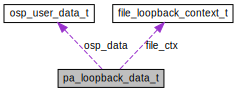
\includegraphics[width=310pt]{structpa__loopback__data__t__coll__graph}
\end{center}
\end{figure}
\subsection*{Data Fields}
\begin{DoxyCompactItemize}
\item 
\mbox{\hyperlink{port__wrapper_8h_a44712da21c339df7c0735d4bab71a303}{file\+\_\+loopback\+\_\+context}} $\ast$ \mbox{\hyperlink{structpa__loopback__data__t_a42a73d3f67c2efae2ed630e67aa8fce9}{file\+\_\+ctx}}
\item 
\mbox{\hyperlink{constants_8h_a2d1d78531fe12807c3852488556d5a4b}{osp\+\_\+user\+\_\+data}} $\ast$ \mbox{\hyperlink{structpa__loopback__data__t_ac17ae97f5292d3ce42b8f35481df55e0}{osp\+\_\+data}}
\item 
unsigned char \mbox{\hyperlink{structpa__loopback__data__t_afcc199ddd9516cf9df956370e5c70482}{done}}
\end{DoxyCompactItemize}


\subsection{Detailed Description}
Wraps around the osp\+\_\+data, but also contains a file loopback context struct Have to wrap the two structs in one data structure so that we can pass it to the Port Audio callback. 

\begin{DoxySeeAlso}{See also}
\mbox{\hyperlink{port__wrapper_8h_a44712da21c339df7c0735d4bab71a303}{file\+\_\+loopback\+\_\+context}} 

\mbox{\hyperlink{constants_8h_a2d1d78531fe12807c3852488556d5a4b}{osp\+\_\+user\+\_\+data}} 
\end{DoxySeeAlso}


\subsection{Field Documentation}
\mbox{\Hypertarget{structpa__loopback__data__t_afcc199ddd9516cf9df956370e5c70482}\label{structpa__loopback__data__t_afcc199ddd9516cf9df956370e5c70482}} 
\index{pa\+\_\+loopback\+\_\+data\+\_\+t@{pa\+\_\+loopback\+\_\+data\+\_\+t}!done@{done}}
\index{done@{done}!pa\+\_\+loopback\+\_\+data\+\_\+t@{pa\+\_\+loopback\+\_\+data\+\_\+t}}
\subsubsection{\texorpdfstring{done}{done}}
{\footnotesize\ttfamily unsigned char pa\+\_\+loopback\+\_\+data\+\_\+t\+::done}

\mbox{\Hypertarget{structpa__loopback__data__t_a42a73d3f67c2efae2ed630e67aa8fce9}\label{structpa__loopback__data__t_a42a73d3f67c2efae2ed630e67aa8fce9}} 
\index{pa\+\_\+loopback\+\_\+data\+\_\+t@{pa\+\_\+loopback\+\_\+data\+\_\+t}!file\+\_\+ctx@{file\+\_\+ctx}}
\index{file\+\_\+ctx@{file\+\_\+ctx}!pa\+\_\+loopback\+\_\+data\+\_\+t@{pa\+\_\+loopback\+\_\+data\+\_\+t}}
\subsubsection{\texorpdfstring{file\+\_\+ctx}{file\_ctx}}
{\footnotesize\ttfamily \mbox{\hyperlink{port__wrapper_8h_a44712da21c339df7c0735d4bab71a303}{file\+\_\+loopback\+\_\+context}}$\ast$ pa\+\_\+loopback\+\_\+data\+\_\+t\+::file\+\_\+ctx}

\mbox{\Hypertarget{structpa__loopback__data__t_ac17ae97f5292d3ce42b8f35481df55e0}\label{structpa__loopback__data__t_ac17ae97f5292d3ce42b8f35481df55e0}} 
\index{pa\+\_\+loopback\+\_\+data\+\_\+t@{pa\+\_\+loopback\+\_\+data\+\_\+t}!osp\+\_\+data@{osp\+\_\+data}}
\index{osp\+\_\+data@{osp\+\_\+data}!pa\+\_\+loopback\+\_\+data\+\_\+t@{pa\+\_\+loopback\+\_\+data\+\_\+t}}
\subsubsection{\texorpdfstring{osp\+\_\+data}{osp\_data}}
{\footnotesize\ttfamily \mbox{\hyperlink{constants_8h_a2d1d78531fe12807c3852488556d5a4b}{osp\+\_\+user\+\_\+data}}$\ast$ pa\+\_\+loopback\+\_\+data\+\_\+t\+::osp\+\_\+data}



The documentation for this struct was generated from the following file\+:\begin{DoxyCompactItemize}
\item 
osp/\mbox{\hyperlink{port__wrapper_8h}{port\+\_\+wrapper.\+h}}\end{DoxyCompactItemize}

\hypertarget{structpa__user__data__t}{}\section{pa\+\_\+user\+\_\+data\+\_\+t Struct Reference}
\label{structpa__user__data__t}\index{pa\+\_\+user\+\_\+data\+\_\+t@{pa\+\_\+user\+\_\+data\+\_\+t}}


The data structure passed to Port\+Audio.  




{\ttfamily \#include $<$constants.\+h$>$}



Collaboration diagram for pa\+\_\+user\+\_\+data\+\_\+t\+:\nopagebreak
\begin{figure}[H]
\begin{center}
\leavevmode
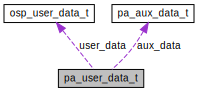
\includegraphics[width=270pt]{structpa__user__data__t__coll__graph}
\end{center}
\end{figure}
\subsection*{Data Fields}
\begin{DoxyCompactItemize}
\item 
\mbox{\hyperlink{constants_8h_a2d1d78531fe12807c3852488556d5a4b}{osp\+\_\+user\+\_\+data}} $\ast$ \mbox{\hyperlink{structpa__user__data__t_afcb50245302828da62e070d923d145c3}{user\+\_\+data}}
\begin{DoxyCompactList}\small\item\em Osp user data struct. \end{DoxyCompactList}\item 
\mbox{\hyperlink{constants_8h_add46628e302aedde68d37aea654eda24}{pa\+\_\+aux\+\_\+data}} \mbox{\hyperlink{structpa__user__data__t_a474dfc8856d57bc28146dbb593147c33}{aux\+\_\+data}}
\begin{DoxyCompactList}\small\item\em Auxiliary struct for misc data. \end{DoxyCompactList}\end{DoxyCompactItemize}


\subsection{Detailed Description}
The data structure passed to Port\+Audio. 

\subsection{Field Documentation}
\mbox{\Hypertarget{structpa__user__data__t_a474dfc8856d57bc28146dbb593147c33}\label{structpa__user__data__t_a474dfc8856d57bc28146dbb593147c33}} 
\index{pa\+\_\+user\+\_\+data\+\_\+t@{pa\+\_\+user\+\_\+data\+\_\+t}!aux\+\_\+data@{aux\+\_\+data}}
\index{aux\+\_\+data@{aux\+\_\+data}!pa\+\_\+user\+\_\+data\+\_\+t@{pa\+\_\+user\+\_\+data\+\_\+t}}
\subsubsection{\texorpdfstring{aux\+\_\+data}{aux\_data}}
{\footnotesize\ttfamily \mbox{\hyperlink{constants_8h_add46628e302aedde68d37aea654eda24}{pa\+\_\+aux\+\_\+data}} pa\+\_\+user\+\_\+data\+\_\+t\+::aux\+\_\+data}



Auxiliary struct for misc data. 

\mbox{\Hypertarget{structpa__user__data__t_afcb50245302828da62e070d923d145c3}\label{structpa__user__data__t_afcb50245302828da62e070d923d145c3}} 
\index{pa\+\_\+user\+\_\+data\+\_\+t@{pa\+\_\+user\+\_\+data\+\_\+t}!user\+\_\+data@{user\+\_\+data}}
\index{user\+\_\+data@{user\+\_\+data}!pa\+\_\+user\+\_\+data\+\_\+t@{pa\+\_\+user\+\_\+data\+\_\+t}}
\subsubsection{\texorpdfstring{user\+\_\+data}{user\_data}}
{\footnotesize\ttfamily \mbox{\hyperlink{constants_8h_a2d1d78531fe12807c3852488556d5a4b}{osp\+\_\+user\+\_\+data}}$\ast$ pa\+\_\+user\+\_\+data\+\_\+t\+::user\+\_\+data}



Osp user data struct. 



The documentation for this struct was generated from the following file\+:\begin{DoxyCompactItemize}
\item 
libosp/common/\mbox{\hyperlink{constants_8h}{constants.\+h}}\end{DoxyCompactItemize}

\hypertarget{structpeak__detect__t}{}\section{peak\+\_\+detect\+\_\+t Struct Reference}
\label{structpeak__detect__t}\index{peak\+\_\+detect\+\_\+t@{peak\+\_\+detect\+\_\+t}}


Peak Detect data structure.  


\subsection*{Data Fields}
\begin{DoxyCompactItemize}
\item 
float \mbox{\hyperlink{structpeak__detect__t_a1d0565d56fe1cef7323916452a05f204}{fsamp}}
\begin{DoxyCompactList}\small\item\em Sampling rate in Hz. \end{DoxyCompactList}\item 
float $\ast$ \mbox{\hyperlink{structpeak__detect__t_a8496e738e882dd4cd75279b874ed9297}{prev\+\_\+peak}}
\begin{DoxyCompactList}\small\item\em Pointer to the array of peak values of the last sample in previous frame for each band. \end{DoxyCompactList}\item 
unsigned int \mbox{\hyperlink{structpeak__detect__t_a18c7ff3dea1f1dafdab996fe12814366}{num\+\_\+bands}}
\begin{DoxyCompactList}\small\item\em Number of sub-\/bands. \end{DoxyCompactList}\end{DoxyCompactItemize}


\subsection{Detailed Description}
Peak Detect data structure. 

\subsection{Field Documentation}
\mbox{\Hypertarget{structpeak__detect__t_a1d0565d56fe1cef7323916452a05f204}\label{structpeak__detect__t_a1d0565d56fe1cef7323916452a05f204}} 
\index{peak\+\_\+detect\+\_\+t@{peak\+\_\+detect\+\_\+t}!fsamp@{fsamp}}
\index{fsamp@{fsamp}!peak\+\_\+detect\+\_\+t@{peak\+\_\+detect\+\_\+t}}
\subsubsection{\texorpdfstring{fsamp}{fsamp}}
{\footnotesize\ttfamily float peak\+\_\+detect\+\_\+t\+::fsamp}



Sampling rate in Hz. 

\mbox{\Hypertarget{structpeak__detect__t_a18c7ff3dea1f1dafdab996fe12814366}\label{structpeak__detect__t_a18c7ff3dea1f1dafdab996fe12814366}} 
\index{peak\+\_\+detect\+\_\+t@{peak\+\_\+detect\+\_\+t}!num\+\_\+bands@{num\+\_\+bands}}
\index{num\+\_\+bands@{num\+\_\+bands}!peak\+\_\+detect\+\_\+t@{peak\+\_\+detect\+\_\+t}}
\subsubsection{\texorpdfstring{num\+\_\+bands}{num\_bands}}
{\footnotesize\ttfamily unsigned int peak\+\_\+detect\+\_\+t\+::num\+\_\+bands}



Number of sub-\/bands. 

\mbox{\Hypertarget{structpeak__detect__t_a8496e738e882dd4cd75279b874ed9297}\label{structpeak__detect__t_a8496e738e882dd4cd75279b874ed9297}} 
\index{peak\+\_\+detect\+\_\+t@{peak\+\_\+detect\+\_\+t}!prev\+\_\+peak@{prev\+\_\+peak}}
\index{prev\+\_\+peak@{prev\+\_\+peak}!peak\+\_\+detect\+\_\+t@{peak\+\_\+detect\+\_\+t}}
\subsubsection{\texorpdfstring{prev\+\_\+peak}{prev\_peak}}
{\footnotesize\ttfamily float$\ast$ peak\+\_\+detect\+\_\+t\+::prev\+\_\+peak}



Pointer to the array of peak values of the last sample in previous frame for each band. 



The documentation for this struct was generated from the following file\+:\begin{DoxyCompactItemize}
\item 
libosp/peak\+\_\+detect/\mbox{\hyperlink{peak__detect_8c}{peak\+\_\+detect.\+c}}\end{DoxyCompactItemize}

\hypertarget{structresample__t}{}\section{resample\+\_\+t Struct Reference}
\label{structresample__t}\index{resample\+\_\+t@{resample\+\_\+t}}


Data struct containing variables for resampler.  




Collaboration diagram for resample\+\_\+t\+:\nopagebreak
\begin{figure}[H]
\begin{center}
\leavevmode
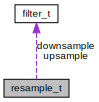
\includegraphics[width=172pt]{structresample__t__coll__graph}
\end{center}
\end{figure}
\subsection*{Data Fields}
\begin{DoxyCompactItemize}
\item 
\mbox{\hyperlink{filter_8h_a69e34b8aa259d2ca0b81b5c95f395bdf}{Filter}} \mbox{\hyperlink{structresample__t_a7f06c113fbaa88f3f943e84358d05e45}{upsample}}
\begin{DoxyCompactList}\small\item\em Upsample filter. \end{DoxyCompactList}\item 
\mbox{\hyperlink{filter_8h_a69e34b8aa259d2ca0b81b5c95f395bdf}{Filter}} \mbox{\hyperlink{structresample__t_a24f8e6d91db22e6809c3be712a0a6437}{downsample}}
\begin{DoxyCompactList}\small\item\em downsample filter \end{DoxyCompactList}\end{DoxyCompactItemize}


\subsection{Detailed Description}
Data struct containing variables for resampler. 

\subsection{Field Documentation}
\mbox{\Hypertarget{structresample__t_a24f8e6d91db22e6809c3be712a0a6437}\label{structresample__t_a24f8e6d91db22e6809c3be712a0a6437}} 
\index{resample\+\_\+t@{resample\+\_\+t}!downsample@{downsample}}
\index{downsample@{downsample}!resample\+\_\+t@{resample\+\_\+t}}
\subsubsection{\texorpdfstring{downsample}{downsample}}
{\footnotesize\ttfamily \mbox{\hyperlink{filter_8h_a69e34b8aa259d2ca0b81b5c95f395bdf}{Filter}} resample\+\_\+t\+::downsample}



downsample filter 

\mbox{\Hypertarget{structresample__t_a7f06c113fbaa88f3f943e84358d05e45}\label{structresample__t_a7f06c113fbaa88f3f943e84358d05e45}} 
\index{resample\+\_\+t@{resample\+\_\+t}!upsample@{upsample}}
\index{upsample@{upsample}!resample\+\_\+t@{resample\+\_\+t}}
\subsubsection{\texorpdfstring{upsample}{upsample}}
{\footnotesize\ttfamily \mbox{\hyperlink{filter_8h_a69e34b8aa259d2ca0b81b5c95f395bdf}{Filter}} resample\+\_\+t\+::upsample}



Upsample filter. 



The documentation for this struct was generated from the following file\+:\begin{DoxyCompactItemize}
\item 
libosp/resample/\mbox{\hyperlink{resample_8c}{resample.\+c}}\end{DoxyCompactItemize}

\chapter{File Documentation}
\hypertarget{afc_8c}{}\section{libosp/afc/afc.c File Reference}
\label{afc_8c}\index{libosp/afc/afc.\+c@{libosp/afc/afc.\+c}}
{\ttfamily \#include $<$stdlib.\+h$>$}\newline
{\ttfamily \#include $<$string.\+h$>$}\newline
{\ttfamily \#include $<$math.\+h$>$}\newline
{\ttfamily \#include \char`\"{}afc.\+h\char`\"{}}\newline
{\ttfamily \#include \char`\"{}filter.\+h\char`\"{}}\newline
{\ttfamily \#include \char`\"{}array\+\_\+utilities.\+h\char`\"{}}\newline
{\ttfamily \#include \char`\"{}circular\+\_\+buffer.\+h\char`\"{}}\newline
Include dependency graph for afc.\+c\+:\nopagebreak
\begin{figure}[H]
\begin{center}
\leavevmode
\includegraphics[width=350pt]{afc_8c__incl}
\end{center}
\end{figure}
\subsection*{Data Structures}
\begin{DoxyCompactItemize}
\item 
struct \mbox{\hyperlink{structafc__t}{afc\+\_\+t}}
\begin{DoxyCompactList}\small\item\em A\+FC data structure. \end{DoxyCompactList}\end{DoxyCompactItemize}
\subsection*{Functions}
\begin{DoxyCompactItemize}
\item 
static void \mbox{\hyperlink{afc_8c_aa954fa18c8519c3b191b6e7e0be8ff02}{compute\+\_\+gradient}} (float $\ast$e\+\_\+prefiltered, float $\ast$u\+\_\+prefiltered\+\_\+accumulated, float $\ast$gradient, size\+\_\+t u\+\_\+prefiltered\+\_\+acc\+\_\+len, size\+\_\+t frame\+\_\+size)
\begin{DoxyCompactList}\small\item\em Compute the gradient for F\+X\+L\+MS update. \end{DoxyCompactList}\item 
void \mbox{\hyperlink{afc_8c_a66ccd7a4405272de4401221d1028b7d2}{D\+S\+P\+F\+\_\+sp\+\_\+fircirc\+\_\+2}} (float x\mbox{[}$\,$\mbox{]}, float h\mbox{[}$\,$\mbox{]}, float r\mbox{[}$\,$\mbox{]}, size\+\_\+t index, size\+\_\+t csize, size\+\_\+t nh, size\+\_\+t nr)
\item 
static void \mbox{\hyperlink{afc_8c_a1eeff5119c14cd963fa967bd209d91d5}{compute\+\_\+gradient\+\_\+upa}} (float $\ast$e\+\_\+prefiltered, \mbox{\hyperlink{circular__buffer_8h_aa88184dd60879f696cb2e679d0e50b45}{Circular\+\_\+buffer}} upa, float $\ast$gradient, size\+\_\+t frame\+\_\+size)
\item 
static void \mbox{\hyperlink{afc_8c_a93d83559cbb9c271e3a8c55a67ffbd09}{update\+\_\+u\+\_\+prefiltered\+\_\+accumulated}} (float $\ast$u\+\_\+prefiltered\+\_\+accumulated, float $\ast$new\+\_\+frame, int u\+\_\+prefiltered\+\_\+acc\+\_\+len, int new\+\_\+frame\+\_\+len)
\begin{DoxyCompactList}\small\item\em Updating u\+\_\+prefiltered\+\_\+accumulated buffer which is circular. \end{DoxyCompactList}\item 
static void \mbox{\hyperlink{afc_8c_a4cfbda46d723acc3423af2483fa0f05a}{get\+\_\+step\+\_\+size\+\_\+weights}} (float $\ast$taps, float $\ast$step\+\_\+size\+\_\+weights, float alpha, float beta, float delta, int len)
\begin{DoxyCompactList}\small\item\em Update the proportionate matrix (P(n)) diagonal matrix for P\+N\+L\+MS adaptation. \end{DoxyCompactList}\item 
\mbox{\hyperlink{afc_8h_a18f5ff6b916f548f1d14d1e48ec23908}{Afc}} \mbox{\hyperlink{afc_8c_ae2ae05e92c452d604e5b283c6db3e307}{afc\+\_\+init}} (const float $\ast$afc\+\_\+filter\+\_\+taps, int afc\+\_\+filter\+\_\+tap\+\_\+len, const float $\ast$prefilter\+\_\+taps, int prefilter\+\_\+tap\+\_\+len, const float $\ast$band\+\_\+limited\+\_\+filter\+\_\+taps, int band\+\_\+limited\+\_\+filter\+\_\+tap\+\_\+len, int frame\+\_\+size, unsigned int adaptation\+\_\+type)
\begin{DoxyCompactList}\small\item\em Function to initialize the afc data struct. \end{DoxyCompactList}\item 
int \mbox{\hyperlink{afc_8c_ac453a669837cff671fbe64d59da8fd03}{afc\+\_\+update\+\_\+taps}} (\mbox{\hyperlink{afc_8h_a18f5ff6b916f548f1d14d1e48ec23908}{Afc}} afc, float $\ast$s, float $\ast$e, size\+\_\+t frame\+\_\+size)
\begin{DoxyCompactList}\small\item\em Function to update the A\+FC filter taps. i.\+e. perform A\+FC. \end{DoxyCompactList}\item 
void \mbox{\hyperlink{afc_8c_ae23fd5ba219af0e472c3ea5a6b883b8e}{afc\+\_\+get\+\_\+y\+\_\+estimated}} (\mbox{\hyperlink{afc_8h_a18f5ff6b916f548f1d14d1e48ec23908}{Afc}} afc, float $\ast$y\+\_\+est, size\+\_\+t len)
\begin{DoxyCompactList}\small\item\em Function to get the estimate of the feedback signal, y\+\_\+hat(n) \end{DoxyCompactList}\item 
int \mbox{\hyperlink{afc_8c_a3b8e35089fac94e704cd9b0a964b7202}{afc\+\_\+get\+\_\+taps}} (\mbox{\hyperlink{afc_8h_a18f5ff6b916f548f1d14d1e48ec23908}{Afc}} afc, float $\ast$taps)
\begin{DoxyCompactList}\small\item\em Function to get the A\+FC filter taps. \end{DoxyCompactList}\item 
int \mbox{\hyperlink{afc_8c_a27cf074c18fa2ff7253bfab542b348cb}{afc\+\_\+destroy}} (\mbox{\hyperlink{afc_8h_a18f5ff6b916f548f1d14d1e48ec23908}{Afc}} afc)
\begin{DoxyCompactList}\small\item\em Function to close and free the Afc instance. \end{DoxyCompactList}\end{DoxyCompactItemize}


\subsection{Function Documentation}
\mbox{\Hypertarget{afc_8c_a27cf074c18fa2ff7253bfab542b348cb}\label{afc_8c_a27cf074c18fa2ff7253bfab542b348cb}} 
\index{afc.\+c@{afc.\+c}!afc\+\_\+destroy@{afc\+\_\+destroy}}
\index{afc\+\_\+destroy@{afc\+\_\+destroy}!afc.\+c@{afc.\+c}}
\subsubsection{\texorpdfstring{afc\+\_\+destroy()}{afc\_destroy()}}
{\footnotesize\ttfamily int afc\+\_\+destroy (\begin{DoxyParamCaption}\item[{\mbox{\hyperlink{afc_8h_a18f5ff6b916f548f1d14d1e48ec23908}{Afc}}}]{afc }\end{DoxyParamCaption})}



Function to close and free the Afc instance. 

\begin{DoxySeeAlso}{See also}
\mbox{\hyperlink{structafc__t}{afc\+\_\+t}} ~\newline

\end{DoxySeeAlso}

\begin{DoxyParams}{Parameters}
{\em afc} & The instance of the Afc structure that was returned from afc\+\_\+init \\
\hline
\end{DoxyParams}
\begin{DoxyReturn}{Returns}
int 0 if successful. -\/1 otherwise 
\end{DoxyReturn}
\mbox{\Hypertarget{afc_8c_a3b8e35089fac94e704cd9b0a964b7202}\label{afc_8c_a3b8e35089fac94e704cd9b0a964b7202}} 
\index{afc.\+c@{afc.\+c}!afc\+\_\+get\+\_\+taps@{afc\+\_\+get\+\_\+taps}}
\index{afc\+\_\+get\+\_\+taps@{afc\+\_\+get\+\_\+taps}!afc.\+c@{afc.\+c}}
\subsubsection{\texorpdfstring{afc\+\_\+get\+\_\+taps()}{afc\_get\_taps()}}
{\footnotesize\ttfamily int afc\+\_\+get\+\_\+taps (\begin{DoxyParamCaption}\item[{\mbox{\hyperlink{afc_8h_a18f5ff6b916f548f1d14d1e48ec23908}{Afc}}}]{afc,  }\item[{float $\ast$}]{taps }\end{DoxyParamCaption})}



Function to get the A\+FC filter taps. 

\begin{DoxySeeAlso}{See also}
\mbox{\hyperlink{structafc__t}{afc\+\_\+t}} ~\newline

\end{DoxySeeAlso}

\begin{DoxyParams}{Parameters}
{\em afc} & The instance of the Afc structure that was returned from afc\+\_\+init \\
\hline
{\em taps} & Pointer to the array that afc filter taps will be written into \\
\hline
\end{DoxyParams}
\begin{DoxyReturn}{Returns}
int A\+FC filter tap length 
\end{DoxyReturn}
\mbox{\Hypertarget{afc_8c_ae23fd5ba219af0e472c3ea5a6b883b8e}\label{afc_8c_ae23fd5ba219af0e472c3ea5a6b883b8e}} 
\index{afc.\+c@{afc.\+c}!afc\+\_\+get\+\_\+y\+\_\+estimated@{afc\+\_\+get\+\_\+y\+\_\+estimated}}
\index{afc\+\_\+get\+\_\+y\+\_\+estimated@{afc\+\_\+get\+\_\+y\+\_\+estimated}!afc.\+c@{afc.\+c}}
\subsubsection{\texorpdfstring{afc\+\_\+get\+\_\+y\+\_\+estimated()}{afc\_get\_y\_estimated()}}
{\footnotesize\ttfamily void afc\+\_\+get\+\_\+y\+\_\+estimated (\begin{DoxyParamCaption}\item[{\mbox{\hyperlink{afc_8h_a18f5ff6b916f548f1d14d1e48ec23908}{Afc}}}]{afc,  }\item[{float $\ast$}]{y\+\_\+est,  }\item[{size\+\_\+t}]{len }\end{DoxyParamCaption})}



Function to get the estimate of the feedback signal, y\+\_\+hat(n) 

\begin{DoxySeeAlso}{See also}
\mbox{\hyperlink{structafc__t}{afc\+\_\+t}} 
\end{DoxySeeAlso}

\begin{DoxyParams}{Parameters}
{\em afc} & The instance of the Afc structure that was returned from afc\+\_\+init \\
\hline
{\em y\+\_\+est} & Pointer to the array that estimated feedback signal will be written into \\
\hline
{\em len} & Number of samples of the estimated feedback signal requested \\
\hline
\end{DoxyParams}
\mbox{\Hypertarget{afc_8c_ae2ae05e92c452d604e5b283c6db3e307}\label{afc_8c_ae2ae05e92c452d604e5b283c6db3e307}} 
\index{afc.\+c@{afc.\+c}!afc\+\_\+init@{afc\+\_\+init}}
\index{afc\+\_\+init@{afc\+\_\+init}!afc.\+c@{afc.\+c}}
\subsubsection{\texorpdfstring{afc\+\_\+init()}{afc\_init()}}
{\footnotesize\ttfamily \mbox{\hyperlink{afc_8h_a18f5ff6b916f548f1d14d1e48ec23908}{Afc}} afc\+\_\+init (\begin{DoxyParamCaption}\item[{const float $\ast$}]{afc\+\_\+filter\+\_\+taps,  }\item[{int}]{afc\+\_\+filter\+\_\+tap\+\_\+len,  }\item[{const float $\ast$}]{prefilter\+\_\+taps,  }\item[{int}]{prefilter\+\_\+tap\+\_\+len,  }\item[{const float $\ast$}]{band\+\_\+limited\+\_\+filter\+\_\+taps,  }\item[{int}]{band\+\_\+limited\+\_\+filter\+\_\+tap\+\_\+len,  }\item[{int}]{frame\+\_\+size,  }\item[{unsigned int}]{adaptation\+\_\+type }\end{DoxyParamCaption})}



Function to initialize the afc data struct. 

Allocates memory to the Afc instance and initialize its parameters.


\begin{DoxyParams}{Parameters}
{\em afc\+\_\+filter\+\_\+taps} & A\+FC filter initalization taps, W(z) initialization \\
\hline
{\em afc\+\_\+filter\+\_\+tap\+\_\+len} & A\+FC filter tap length \\
\hline
{\em prefilter\+\_\+taps} & Pre-\/whitening filter taps, A(z) \\
\hline
{\em prefilter\+\_\+tap\+\_\+len} & Pre-\/whitening filter tap length \\
\hline
{\em band\+\_\+limited\+\_\+filter\+\_\+taps} & Band-\/limited filter taps, H(z) \\
\hline
{\em band\+\_\+limited\+\_\+filter\+\_\+tap\+\_\+len} & Band-\/limited filter tap length \\
\hline
{\em frame\+\_\+size} & Frame size to process \\
\hline
{\em adaptation\+\_\+type} & A\+FC adaptation type. 1 = (F\+X\+L\+MS + P\+N\+L\+MS), 0 = F\+X\+L\+MS \\
\hline
\end{DoxyParams}
\begin{DoxyReturn}{Returns}
Afc Returns the Afc instance/object if memory is succesfully allocated or returns N\+U\+LL. 
\end{DoxyReturn}
\mbox{\Hypertarget{afc_8c_ac453a669837cff671fbe64d59da8fd03}\label{afc_8c_ac453a669837cff671fbe64d59da8fd03}} 
\index{afc.\+c@{afc.\+c}!afc\+\_\+update\+\_\+taps@{afc\+\_\+update\+\_\+taps}}
\index{afc\+\_\+update\+\_\+taps@{afc\+\_\+update\+\_\+taps}!afc.\+c@{afc.\+c}}
\subsubsection{\texorpdfstring{afc\+\_\+update\+\_\+taps()}{afc\_update\_taps()}}
{\footnotesize\ttfamily int afc\+\_\+update\+\_\+taps (\begin{DoxyParamCaption}\item[{\mbox{\hyperlink{afc_8h_a18f5ff6b916f548f1d14d1e48ec23908}{Afc}}}]{afc,  }\item[{float $\ast$}]{s,  }\item[{float $\ast$}]{e,  }\item[{size\+\_\+t}]{frame\+\_\+size }\end{DoxyParamCaption})}



Function to update the A\+FC filter taps. i.\+e. perform A\+FC. 

\begin{DoxySeeAlso}{See also}
\mbox{\hyperlink{structafc__t}{afc\+\_\+t}} 
\end{DoxySeeAlso}

\begin{DoxyParams}{Parameters}
{\em afc} & The instance of the Afc structure that was returned from afc\+\_\+init ~\newline
\\
\hline
{\em s} & Pointer to the output signal array of W\+D\+RC \\
\hline
{\em e} & Pointer to the error signal array \\
\hline
{\em frame\+\_\+size} & Number of samples in the frame to process \\
\hline
\end{DoxyParams}
\begin{DoxyReturn}{Returns}
int -\/1 for wrong frame size. 0 if successful 
\end{DoxyReturn}
\mbox{\Hypertarget{afc_8c_aa954fa18c8519c3b191b6e7e0be8ff02}\label{afc_8c_aa954fa18c8519c3b191b6e7e0be8ff02}} 
\index{afc.\+c@{afc.\+c}!compute\+\_\+gradient@{compute\+\_\+gradient}}
\index{compute\+\_\+gradient@{compute\+\_\+gradient}!afc.\+c@{afc.\+c}}
\subsubsection{\texorpdfstring{compute\+\_\+gradient()}{compute\_gradient()}}
{\footnotesize\ttfamily static void compute\+\_\+gradient (\begin{DoxyParamCaption}\item[{float $\ast$}]{e\+\_\+prefiltered,  }\item[{float $\ast$}]{u\+\_\+prefiltered\+\_\+accumulated,  }\item[{float $\ast$}]{gradient,  }\item[{size\+\_\+t}]{u\+\_\+prefiltered\+\_\+acc\+\_\+len,  }\item[{size\+\_\+t}]{frame\+\_\+size }\end{DoxyParamCaption})\hspace{0.3cm}{\ttfamily [static]}}



Compute the gradient for F\+X\+L\+MS update. 


\begin{DoxyParams}{Parameters}
{\em e\+\_\+prefiltered} & Pointer to the array containing pre-\/filtered input e\+\_\+f(n) \\
\hline
{\em u\+\_\+prefiltered\+\_\+accumulated} & Pointer to the buffer of accumulated values of pre-\/filtered output of u(n) i.\+e., u\+\_\+f(n) \\
\hline
{\em gradient} & Pointer to the array where the gradient will be written into \\
\hline
{\em u\+\_\+prefiltered\+\_\+acc\+\_\+len} & Length of the u\+\_\+prefiltered\+\_\+accumulated buffer \\
\hline
{\em frame\+\_\+size} & Length of the frame size which is also the length of e\+\_\+prefiltered \\
\hline
\end{DoxyParams}
\mbox{\Hypertarget{afc_8c_a1eeff5119c14cd963fa967bd209d91d5}\label{afc_8c_a1eeff5119c14cd963fa967bd209d91d5}} 
\index{afc.\+c@{afc.\+c}!compute\+\_\+gradient\+\_\+upa@{compute\+\_\+gradient\+\_\+upa}}
\index{compute\+\_\+gradient\+\_\+upa@{compute\+\_\+gradient\+\_\+upa}!afc.\+c@{afc.\+c}}
\subsubsection{\texorpdfstring{compute\+\_\+gradient\+\_\+upa()}{compute\_gradient\_upa()}}
{\footnotesize\ttfamily static void compute\+\_\+gradient\+\_\+upa (\begin{DoxyParamCaption}\item[{float $\ast$}]{e\+\_\+prefiltered,  }\item[{\mbox{\hyperlink{circular__buffer_8h_aa88184dd60879f696cb2e679d0e50b45}{Circular\+\_\+buffer}}}]{upa,  }\item[{float $\ast$}]{gradient,  }\item[{size\+\_\+t}]{frame\+\_\+size }\end{DoxyParamCaption})\hspace{0.3cm}{\ttfamily [static]}}

\mbox{\Hypertarget{afc_8c_a66ccd7a4405272de4401221d1028b7d2}\label{afc_8c_a66ccd7a4405272de4401221d1028b7d2}} 
\index{afc.\+c@{afc.\+c}!D\+S\+P\+F\+\_\+sp\+\_\+fircirc\+\_\+2@{D\+S\+P\+F\+\_\+sp\+\_\+fircirc\+\_\+2}}
\index{D\+S\+P\+F\+\_\+sp\+\_\+fircirc\+\_\+2@{D\+S\+P\+F\+\_\+sp\+\_\+fircirc\+\_\+2}!afc.\+c@{afc.\+c}}
\subsubsection{\texorpdfstring{D\+S\+P\+F\+\_\+sp\+\_\+fircirc\+\_\+2()}{DSPF\_sp\_fircirc\_2()}}
{\footnotesize\ttfamily void D\+S\+P\+F\+\_\+sp\+\_\+fircirc\+\_\+2 (\begin{DoxyParamCaption}\item[{float}]{x\mbox{[}$\,$\mbox{]},  }\item[{float}]{h\mbox{[}$\,$\mbox{]},  }\item[{float}]{r\mbox{[}$\,$\mbox{]},  }\item[{size\+\_\+t}]{index,  }\item[{size\+\_\+t}]{csize,  }\item[{size\+\_\+t}]{nh,  }\item[{size\+\_\+t}]{nr }\end{DoxyParamCaption})}

\mbox{\Hypertarget{afc_8c_a4cfbda46d723acc3423af2483fa0f05a}\label{afc_8c_a4cfbda46d723acc3423af2483fa0f05a}} 
\index{afc.\+c@{afc.\+c}!get\+\_\+step\+\_\+size\+\_\+weights@{get\+\_\+step\+\_\+size\+\_\+weights}}
\index{get\+\_\+step\+\_\+size\+\_\+weights@{get\+\_\+step\+\_\+size\+\_\+weights}!afc.\+c@{afc.\+c}}
\subsubsection{\texorpdfstring{get\+\_\+step\+\_\+size\+\_\+weights()}{get\_step\_size\_weights()}}
{\footnotesize\ttfamily static void get\+\_\+step\+\_\+size\+\_\+weights (\begin{DoxyParamCaption}\item[{float $\ast$}]{taps,  }\item[{float $\ast$}]{step\+\_\+size\+\_\+weights,  }\item[{float}]{alpha,  }\item[{float}]{beta,  }\item[{float}]{delta,  }\item[{int}]{len }\end{DoxyParamCaption})\hspace{0.3cm}{\ttfamily [static]}}



Update the proportionate matrix (P(n)) diagonal matrix for P\+N\+L\+MS adaptation. 

Get weights for all step sizes. Step sizes are different for each filter tap


\begin{DoxyParams}{Parameters}
{\em taps} & Pointer to the array that contain A\+FC filter taps \\
\hline
{\em step\+\_\+size\+\_\+weights} & Pointer to the array that step size weights will be written into \\
\hline
{\em alpha} & Parameter for P\+N\+L\+MS \\
\hline
{\em beta} & Parameter for P\+N\+L\+MS \\
\hline
{\em delta} & Regularization parameter \\
\hline
{\em len} & Length of the A\+FC filter \\
\hline
\end{DoxyParams}
\mbox{\Hypertarget{afc_8c_a93d83559cbb9c271e3a8c55a67ffbd09}\label{afc_8c_a93d83559cbb9c271e3a8c55a67ffbd09}} 
\index{afc.\+c@{afc.\+c}!update\+\_\+u\+\_\+prefiltered\+\_\+accumulated@{update\+\_\+u\+\_\+prefiltered\+\_\+accumulated}}
\index{update\+\_\+u\+\_\+prefiltered\+\_\+accumulated@{update\+\_\+u\+\_\+prefiltered\+\_\+accumulated}!afc.\+c@{afc.\+c}}
\subsubsection{\texorpdfstring{update\+\_\+u\+\_\+prefiltered\+\_\+accumulated()}{update\_u\_prefiltered\_accumulated()}}
{\footnotesize\ttfamily static void update\+\_\+u\+\_\+prefiltered\+\_\+accumulated (\begin{DoxyParamCaption}\item[{float $\ast$}]{u\+\_\+prefiltered\+\_\+accumulated,  }\item[{float $\ast$}]{new\+\_\+frame,  }\item[{int}]{u\+\_\+prefiltered\+\_\+acc\+\_\+len,  }\item[{int}]{new\+\_\+frame\+\_\+len }\end{DoxyParamCaption})\hspace{0.3cm}{\ttfamily [static]}}



Updating u\+\_\+prefiltered\+\_\+accumulated buffer which is circular. 

Replace the frame\+\_\+size number of old values with new values in the circular buffer using the last element of the buffer as the start index.


\begin{DoxyParams}{Parameters}
{\em u\+\_\+prefiltered\+\_\+accumulated} & Pointer to the buffer of accumulated values of pre-\/filtered output of u(n) i.\+e., u\+\_\+f(n) \\
\hline
{\em new\+\_\+frame} & Pointer to the pre-\/filtered output of u(n) for the new frame \\
\hline
{\em u\+\_\+prefiltered\+\_\+acc\+\_\+len} & Length of the u\+\_\+prefiltered\+\_\+accumulated buffer \\
\hline
{\em new\+\_\+frame\+\_\+len} & Length of new\+\_\+frame which is equal to the frame\+\_\+size \\
\hline
\end{DoxyParams}

\hypertarget{afc_8h}{}\section{libosp/afc/afc.h File Reference}
\label{afc_8h}\index{libosp/afc/afc.\+h@{libosp/afc/afc.\+h}}
This graph shows which files directly or indirectly include this file\+:\nopagebreak
\begin{figure}[H]
\begin{center}
\leavevmode
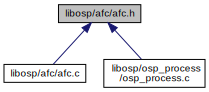
\includegraphics[width=282pt]{afc_8h__dep__incl}
\end{center}
\end{figure}
\subsection*{Macros}
\begin{DoxyCompactItemize}
\item 
\#define \mbox{\hyperlink{afc_8h_a56a54cded994eb84c93ab352ead9d95f}{A\+F\+C\+\_\+\+N\+U\+M\+\_\+\+F\+R\+A\+M\+ES}}~7
\begin{DoxyCompactList}\small\item\em Amount of frames required for A\+FC processing. \end{DoxyCompactList}\item 
\#define \mbox{\hyperlink{afc_8h_a03268366c1b4b6ba55f87a5786ecf00a}{A\+F\+C\+\_\+\+F\+I\+L\+T\+E\+R\+\_\+\+T\+A\+P\+\_\+\+L\+EN}}~192
\begin{DoxyCompactList}\small\item\em A\+FC fitler tap length. \end{DoxyCompactList}\item 
\#define \mbox{\hyperlink{afc_8h_a6242a25f9d996f0cc4f4cdb911218b75}{A\+R\+R\+A\+Y\+\_\+\+S\+I\+ZE}}(x)~(sizeof((x)) / sizeof((x)\mbox{[}0\mbox{]}))
\end{DoxyCompactItemize}
\subsection*{Typedefs}
\begin{DoxyCompactItemize}
\item 
typedef struct \mbox{\hyperlink{structafc__t}{afc\+\_\+t}} $\ast$ \mbox{\hyperlink{afc_8h_a18f5ff6b916f548f1d14d1e48ec23908}{Afc}}
\end{DoxyCompactItemize}
\subsection*{Functions}
\begin{DoxyCompactItemize}
\item 
\mbox{\hyperlink{afc_8h_a18f5ff6b916f548f1d14d1e48ec23908}{Afc}} \mbox{\hyperlink{afc_8h_abe05d4f7f9d83b91231162a853c8bfef}{afc\+\_\+init}} (const float $\ast$afc\+\_\+filter\+\_\+taps, int afc\+\_\+filter\+\_\+tap\+\_\+len, const float $\ast$prefilter\+\_\+taps, int prefilter\+\_\+tap\+\_\+len, const float $\ast$band\+\_\+limited\+\_\+filter\+\_\+taps, int band\+\_\+limited\+\_\+filter\+\_\+tap\+\_\+len, int frame\+\_\+size, unsigned int adaptation\+\_\+type, float afc\+\_\+mu, float afc\+\_\+rho)
\begin{DoxyCompactList}\small\item\em Function to initialize the afc data struct. \end{DoxyCompactList}\item 
int \mbox{\hyperlink{afc_8h_ac453a669837cff671fbe64d59da8fd03}{afc\+\_\+update\+\_\+taps}} (\mbox{\hyperlink{afc_8h_a18f5ff6b916f548f1d14d1e48ec23908}{Afc}} afc, float $\ast$s, float $\ast$e, size\+\_\+t frame\+\_\+size)
\begin{DoxyCompactList}\small\item\em Function to update the A\+FC filter taps. i.\+e. perform A\+FC. \end{DoxyCompactList}\item 
void \mbox{\hyperlink{afc_8h_ae23fd5ba219af0e472c3ea5a6b883b8e}{afc\+\_\+get\+\_\+y\+\_\+estimated}} (\mbox{\hyperlink{afc_8h_a18f5ff6b916f548f1d14d1e48ec23908}{Afc}} afc, float $\ast$y\+\_\+est, size\+\_\+t len)
\begin{DoxyCompactList}\small\item\em Function to get the estimate of the feedback signal, y\+\_\+hat(n) \end{DoxyCompactList}\item 
int \mbox{\hyperlink{afc_8h_a3b8e35089fac94e704cd9b0a964b7202}{afc\+\_\+get\+\_\+taps}} (\mbox{\hyperlink{afc_8h_a18f5ff6b916f548f1d14d1e48ec23908}{Afc}} afc, float $\ast$taps)
\begin{DoxyCompactList}\small\item\em Function to get the A\+FC filter taps. \end{DoxyCompactList}\item 
int \mbox{\hyperlink{afc_8h_a27cf074c18fa2ff7253bfab542b348cb}{afc\+\_\+destroy}} (\mbox{\hyperlink{afc_8h_a18f5ff6b916f548f1d14d1e48ec23908}{Afc}} afc)
\begin{DoxyCompactList}\small\item\em Function to close and free the Afc instance. \end{DoxyCompactList}\end{DoxyCompactItemize}


\subsection{Macro Definition Documentation}
\mbox{\Hypertarget{afc_8h_a03268366c1b4b6ba55f87a5786ecf00a}\label{afc_8h_a03268366c1b4b6ba55f87a5786ecf00a}} 
\index{afc.\+h@{afc.\+h}!A\+F\+C\+\_\+\+F\+I\+L\+T\+E\+R\+\_\+\+T\+A\+P\+\_\+\+L\+EN@{A\+F\+C\+\_\+\+F\+I\+L\+T\+E\+R\+\_\+\+T\+A\+P\+\_\+\+L\+EN}}
\index{A\+F\+C\+\_\+\+F\+I\+L\+T\+E\+R\+\_\+\+T\+A\+P\+\_\+\+L\+EN@{A\+F\+C\+\_\+\+F\+I\+L\+T\+E\+R\+\_\+\+T\+A\+P\+\_\+\+L\+EN}!afc.\+h@{afc.\+h}}
\subsubsection{\texorpdfstring{A\+F\+C\+\_\+\+F\+I\+L\+T\+E\+R\+\_\+\+T\+A\+P\+\_\+\+L\+EN}{AFC\_FILTER\_TAP\_LEN}}
{\footnotesize\ttfamily \#define A\+F\+C\+\_\+\+F\+I\+L\+T\+E\+R\+\_\+\+T\+A\+P\+\_\+\+L\+EN~192}



A\+FC fitler tap length. 

\mbox{\Hypertarget{afc_8h_a56a54cded994eb84c93ab352ead9d95f}\label{afc_8h_a56a54cded994eb84c93ab352ead9d95f}} 
\index{afc.\+h@{afc.\+h}!A\+F\+C\+\_\+\+N\+U\+M\+\_\+\+F\+R\+A\+M\+ES@{A\+F\+C\+\_\+\+N\+U\+M\+\_\+\+F\+R\+A\+M\+ES}}
\index{A\+F\+C\+\_\+\+N\+U\+M\+\_\+\+F\+R\+A\+M\+ES@{A\+F\+C\+\_\+\+N\+U\+M\+\_\+\+F\+R\+A\+M\+ES}!afc.\+h@{afc.\+h}}
\subsubsection{\texorpdfstring{A\+F\+C\+\_\+\+N\+U\+M\+\_\+\+F\+R\+A\+M\+ES}{AFC\_NUM\_FRAMES}}
{\footnotesize\ttfamily \#define A\+F\+C\+\_\+\+N\+U\+M\+\_\+\+F\+R\+A\+M\+ES~7}



Amount of frames required for A\+FC processing. 

\mbox{\Hypertarget{afc_8h_a6242a25f9d996f0cc4f4cdb911218b75}\label{afc_8h_a6242a25f9d996f0cc4f4cdb911218b75}} 
\index{afc.\+h@{afc.\+h}!A\+R\+R\+A\+Y\+\_\+\+S\+I\+ZE@{A\+R\+R\+A\+Y\+\_\+\+S\+I\+ZE}}
\index{A\+R\+R\+A\+Y\+\_\+\+S\+I\+ZE@{A\+R\+R\+A\+Y\+\_\+\+S\+I\+ZE}!afc.\+h@{afc.\+h}}
\subsubsection{\texorpdfstring{A\+R\+R\+A\+Y\+\_\+\+S\+I\+ZE}{ARRAY\_SIZE}}
{\footnotesize\ttfamily \#define A\+R\+R\+A\+Y\+\_\+\+S\+I\+ZE(\begin{DoxyParamCaption}\item[{}]{x }\end{DoxyParamCaption})~(sizeof((x)) / sizeof((x)\mbox{[}0\mbox{]}))}



\subsection{Typedef Documentation}
\mbox{\Hypertarget{afc_8h_a18f5ff6b916f548f1d14d1e48ec23908}\label{afc_8h_a18f5ff6b916f548f1d14d1e48ec23908}} 
\index{afc.\+h@{afc.\+h}!Afc@{Afc}}
\index{Afc@{Afc}!afc.\+h@{afc.\+h}}
\subsubsection{\texorpdfstring{Afc}{Afc}}
{\footnotesize\ttfamily typedef struct \mbox{\hyperlink{structafc__t}{afc\+\_\+t}}$\ast$ \mbox{\hyperlink{afc_8h_a18f5ff6b916f548f1d14d1e48ec23908}{Afc}}}



\subsection{Function Documentation}
\mbox{\Hypertarget{afc_8h_a27cf074c18fa2ff7253bfab542b348cb}\label{afc_8h_a27cf074c18fa2ff7253bfab542b348cb}} 
\index{afc.\+h@{afc.\+h}!afc\+\_\+destroy@{afc\+\_\+destroy}}
\index{afc\+\_\+destroy@{afc\+\_\+destroy}!afc.\+h@{afc.\+h}}
\subsubsection{\texorpdfstring{afc\+\_\+destroy()}{afc\_destroy()}}
{\footnotesize\ttfamily int afc\+\_\+destroy (\begin{DoxyParamCaption}\item[{\mbox{\hyperlink{afc_8h_a18f5ff6b916f548f1d14d1e48ec23908}{Afc}}}]{afc }\end{DoxyParamCaption})}



Function to close and free the Afc instance. 

\begin{DoxySeeAlso}{See also}
\mbox{\hyperlink{structafc__t}{afc\+\_\+t}} ~\newline

\end{DoxySeeAlso}

\begin{DoxyParams}{Parameters}
{\em afc} & The instance of the Afc structure that was returned from afc\+\_\+init \\
\hline
\end{DoxyParams}
\begin{DoxyReturn}{Returns}
int 0 if successful. -\/1 otherwise 
\end{DoxyReturn}
\mbox{\Hypertarget{afc_8h_a3b8e35089fac94e704cd9b0a964b7202}\label{afc_8h_a3b8e35089fac94e704cd9b0a964b7202}} 
\index{afc.\+h@{afc.\+h}!afc\+\_\+get\+\_\+taps@{afc\+\_\+get\+\_\+taps}}
\index{afc\+\_\+get\+\_\+taps@{afc\+\_\+get\+\_\+taps}!afc.\+h@{afc.\+h}}
\subsubsection{\texorpdfstring{afc\+\_\+get\+\_\+taps()}{afc\_get\_taps()}}
{\footnotesize\ttfamily int afc\+\_\+get\+\_\+taps (\begin{DoxyParamCaption}\item[{\mbox{\hyperlink{afc_8h_a18f5ff6b916f548f1d14d1e48ec23908}{Afc}}}]{afc,  }\item[{float $\ast$}]{taps }\end{DoxyParamCaption})}



Function to get the A\+FC filter taps. 

\begin{DoxySeeAlso}{See also}
\mbox{\hyperlink{structafc__t}{afc\+\_\+t}} ~\newline

\end{DoxySeeAlso}

\begin{DoxyParams}{Parameters}
{\em afc} & The instance of the Afc structure that was returned from afc\+\_\+init \\
\hline
{\em taps} & Pointer to the array that afc filter taps will be written into \\
\hline
\end{DoxyParams}
\begin{DoxyReturn}{Returns}
int A\+FC filter tap length 
\end{DoxyReturn}
\mbox{\Hypertarget{afc_8h_ae23fd5ba219af0e472c3ea5a6b883b8e}\label{afc_8h_ae23fd5ba219af0e472c3ea5a6b883b8e}} 
\index{afc.\+h@{afc.\+h}!afc\+\_\+get\+\_\+y\+\_\+estimated@{afc\+\_\+get\+\_\+y\+\_\+estimated}}
\index{afc\+\_\+get\+\_\+y\+\_\+estimated@{afc\+\_\+get\+\_\+y\+\_\+estimated}!afc.\+h@{afc.\+h}}
\subsubsection{\texorpdfstring{afc\+\_\+get\+\_\+y\+\_\+estimated()}{afc\_get\_y\_estimated()}}
{\footnotesize\ttfamily void afc\+\_\+get\+\_\+y\+\_\+estimated (\begin{DoxyParamCaption}\item[{\mbox{\hyperlink{afc_8h_a18f5ff6b916f548f1d14d1e48ec23908}{Afc}}}]{afc,  }\item[{float $\ast$}]{y\+\_\+est,  }\item[{size\+\_\+t}]{len }\end{DoxyParamCaption})}



Function to get the estimate of the feedback signal, y\+\_\+hat(n) 

\begin{DoxySeeAlso}{See also}
\mbox{\hyperlink{structafc__t}{afc\+\_\+t}} 
\end{DoxySeeAlso}

\begin{DoxyParams}{Parameters}
{\em afc} & The instance of the Afc structure that was returned from afc\+\_\+init \\
\hline
{\em y\+\_\+est} & Pointer to the array that estimated feedback signal will be written into \\
\hline
{\em len} & Number of samples of the estimated feedback signal requested \\
\hline
\end{DoxyParams}
\mbox{\Hypertarget{afc_8h_abe05d4f7f9d83b91231162a853c8bfef}\label{afc_8h_abe05d4f7f9d83b91231162a853c8bfef}} 
\index{afc.\+h@{afc.\+h}!afc\+\_\+init@{afc\+\_\+init}}
\index{afc\+\_\+init@{afc\+\_\+init}!afc.\+h@{afc.\+h}}
\subsubsection{\texorpdfstring{afc\+\_\+init()}{afc\_init()}}
{\footnotesize\ttfamily \mbox{\hyperlink{afc_8h_a18f5ff6b916f548f1d14d1e48ec23908}{Afc}} afc\+\_\+init (\begin{DoxyParamCaption}\item[{const float $\ast$}]{afc\+\_\+filter\+\_\+taps,  }\item[{int}]{afc\+\_\+filter\+\_\+tap\+\_\+len,  }\item[{const float $\ast$}]{prefilter\+\_\+taps,  }\item[{int}]{prefilter\+\_\+tap\+\_\+len,  }\item[{const float $\ast$}]{band\+\_\+limited\+\_\+filter\+\_\+taps,  }\item[{int}]{band\+\_\+limited\+\_\+filter\+\_\+tap\+\_\+len,  }\item[{int}]{frame\+\_\+size,  }\item[{unsigned int}]{adaptation\+\_\+type,  }\item[{float}]{afc\+\_\+mu,  }\item[{float}]{afc\+\_\+rho }\end{DoxyParamCaption})}



Function to initialize the afc data struct. 

Allocates memory to the Afc instance and initialize its parameters.


\begin{DoxyParams}{Parameters}
{\em afc\+\_\+filter\+\_\+taps} & A\+FC filter initalization taps, W(z) initialization \\
\hline
{\em afc\+\_\+filter\+\_\+tap\+\_\+len} & A\+FC filter tap length \\
\hline
{\em prefilter\+\_\+taps} & Pre-\/whitening filter taps, A(z) \\
\hline
{\em prefilter\+\_\+tap\+\_\+len} & Pre-\/whitening filter tap length \\
\hline
{\em band\+\_\+limited\+\_\+filter\+\_\+taps} & Band-\/limited filter taps, H(z) \\
\hline
{\em band\+\_\+limited\+\_\+filter\+\_\+tap\+\_\+len} & Band-\/limited filter tap length \\
\hline
{\em frame\+\_\+size} & Frame size to process \\
\hline
{\em adaptation\+\_\+type} & A\+FC adaptation type. 1 = (F\+X\+L\+MS + P\+N\+L\+MS), 0 = F\+X\+L\+MS \\
\hline
\end{DoxyParams}
\begin{DoxyReturn}{Returns}
Afc Returns the Afc instance/object if memory is succesfully allocated or returns N\+U\+LL. 
\end{DoxyReturn}
\mbox{\Hypertarget{afc_8h_ac453a669837cff671fbe64d59da8fd03}\label{afc_8h_ac453a669837cff671fbe64d59da8fd03}} 
\index{afc.\+h@{afc.\+h}!afc\+\_\+update\+\_\+taps@{afc\+\_\+update\+\_\+taps}}
\index{afc\+\_\+update\+\_\+taps@{afc\+\_\+update\+\_\+taps}!afc.\+h@{afc.\+h}}
\subsubsection{\texorpdfstring{afc\+\_\+update\+\_\+taps()}{afc\_update\_taps()}}
{\footnotesize\ttfamily int afc\+\_\+update\+\_\+taps (\begin{DoxyParamCaption}\item[{\mbox{\hyperlink{afc_8h_a18f5ff6b916f548f1d14d1e48ec23908}{Afc}}}]{afc,  }\item[{float $\ast$}]{s,  }\item[{float $\ast$}]{e,  }\item[{size\+\_\+t}]{frame\+\_\+size }\end{DoxyParamCaption})}



Function to update the A\+FC filter taps. i.\+e. perform A\+FC. 

\begin{DoxySeeAlso}{See also}
\mbox{\hyperlink{structafc__t}{afc\+\_\+t}} 
\end{DoxySeeAlso}

\begin{DoxyParams}{Parameters}
{\em afc} & The instance of the Afc structure that was returned from afc\+\_\+init ~\newline
\\
\hline
{\em s} & Pointer to the output signal array of W\+D\+RC \\
\hline
{\em e} & Pointer to the error signal array \\
\hline
{\em frame\+\_\+size} & Number of samples in the frame to process \\
\hline
\end{DoxyParams}
\begin{DoxyReturn}{Returns}
int -\/1 for wrong frame size. 0 if successful 
\end{DoxyReturn}

\input{circular__buffer_8c}
\hypertarget{circular__buffer_8h}{}\section{libosp/afc/circular\+\_\+buffer.h File Reference}
\label{circular__buffer_8h}\index{libosp/afc/circular\+\_\+buffer.\+h@{libosp/afc/circular\+\_\+buffer.\+h}}
This graph shows which files directly or indirectly include this file\+:\nopagebreak
\begin{figure}[H]
\begin{center}
\leavevmode
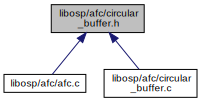
\includegraphics[width=274pt]{circular__buffer_8h__dep__incl}
\end{center}
\end{figure}
\subsection*{Typedefs}
\begin{DoxyCompactItemize}
\item 
typedef struct \mbox{\hyperlink{structcircular__buffer__t}{circular\+\_\+buffer\+\_\+t}} $\ast$ \mbox{\hyperlink{circular__buffer_8h_aa88184dd60879f696cb2e679d0e50b45}{Circular\+\_\+buffer}}
\end{DoxyCompactItemize}
\subsection*{Functions}
\begin{DoxyCompactItemize}
\item 
\mbox{\hyperlink{circular__buffer_8h_aa88184dd60879f696cb2e679d0e50b45}{Circular\+\_\+buffer}} \mbox{\hyperlink{circular__buffer_8h_ae854a1e8bed32b261a78a91a3a849480}{circular\+\_\+buffer\+\_\+init}} (size\+\_\+t buf\+\_\+len)
\item 
int \mbox{\hyperlink{circular__buffer_8h_aaeb0db4fcd28eda0597f1747012c36fb}{circular\+\_\+buffer\+\_\+update\+\_\+buffer}} (\mbox{\hyperlink{circular__buffer_8h_aa88184dd60879f696cb2e679d0e50b45}{Circular\+\_\+buffer}} obj, float $\ast$new\+\_\+vals, size\+\_\+t new\+\_\+vals\+\_\+len)
\item 
size\+\_\+t \mbox{\hyperlink{circular__buffer_8h_a6c51cdfdc4c25f6284b69996f0e6e264}{circular\+\_\+buffer\+\_\+get\+\_\+internal\+\_\+buffer}} (\mbox{\hyperlink{circular__buffer_8h_aa88184dd60879f696cb2e679d0e50b45}{Circular\+\_\+buffer}} obj, float $\ast$buf)
\item 
void \mbox{\hyperlink{circular__buffer_8h_a5f93a58a4828476bf3aa1528109f8f0c}{circular\+\_\+buffer\+\_\+flush}} (\mbox{\hyperlink{circular__buffer_8h_aa88184dd60879f696cb2e679d0e50b45}{Circular\+\_\+buffer}} obj, float $\ast$out)
\item 
int \mbox{\hyperlink{circular__buffer_8h_a70dd7f1d4663218af3a7a31a523c03e2}{circular\+\_\+buffer\+\_\+destroy}} (\mbox{\hyperlink{circular__buffer_8h_aa88184dd60879f696cb2e679d0e50b45}{Circular\+\_\+buffer}} obj)
\item 
size\+\_\+t \mbox{\hyperlink{circular__buffer_8h_a1e9b422b65dca1b57e0c1a03a284eebe}{circular\+\_\+buffer\+\_\+get\+\_\+buffer\+\_\+size}} (\mbox{\hyperlink{circular__buffer_8h_aa88184dd60879f696cb2e679d0e50b45}{Circular\+\_\+buffer}} obj)
\item 
unsigned char \mbox{\hyperlink{circular__buffer_8h_a0ad417236b282aa51453acb29b2d8257}{circular\+\_\+buffer\+\_\+get\+\_\+exp}} (\mbox{\hyperlink{circular__buffer_8h_aa88184dd60879f696cb2e679d0e50b45}{Circular\+\_\+buffer}} obj)
\end{DoxyCompactItemize}


\subsection{Typedef Documentation}
\mbox{\Hypertarget{circular__buffer_8h_aa88184dd60879f696cb2e679d0e50b45}\label{circular__buffer_8h_aa88184dd60879f696cb2e679d0e50b45}} 
\index{circular\+\_\+buffer.\+h@{circular\+\_\+buffer.\+h}!Circular\+\_\+buffer@{Circular\+\_\+buffer}}
\index{Circular\+\_\+buffer@{Circular\+\_\+buffer}!circular\+\_\+buffer.\+h@{circular\+\_\+buffer.\+h}}
\subsubsection{\texorpdfstring{Circular\+\_\+buffer}{Circular\_buffer}}
{\footnotesize\ttfamily typedef struct \mbox{\hyperlink{structcircular__buffer__t}{circular\+\_\+buffer\+\_\+t}}$\ast$ \mbox{\hyperlink{circular__buffer_8h_aa88184dd60879f696cb2e679d0e50b45}{Circular\+\_\+buffer}}}



\subsection{Function Documentation}
\mbox{\Hypertarget{circular__buffer_8h_a70dd7f1d4663218af3a7a31a523c03e2}\label{circular__buffer_8h_a70dd7f1d4663218af3a7a31a523c03e2}} 
\index{circular\+\_\+buffer.\+h@{circular\+\_\+buffer.\+h}!circular\+\_\+buffer\+\_\+destroy@{circular\+\_\+buffer\+\_\+destroy}}
\index{circular\+\_\+buffer\+\_\+destroy@{circular\+\_\+buffer\+\_\+destroy}!circular\+\_\+buffer.\+h@{circular\+\_\+buffer.\+h}}
\subsubsection{\texorpdfstring{circular\+\_\+buffer\+\_\+destroy()}{circular\_buffer\_destroy()}}
{\footnotesize\ttfamily int circular\+\_\+buffer\+\_\+destroy (\begin{DoxyParamCaption}\item[{\mbox{\hyperlink{circular__buffer_8h_aa88184dd60879f696cb2e679d0e50b45}{Circular\+\_\+buffer}}}]{obj }\end{DoxyParamCaption})}

\mbox{\Hypertarget{circular__buffer_8h_a5f93a58a4828476bf3aa1528109f8f0c}\label{circular__buffer_8h_a5f93a58a4828476bf3aa1528109f8f0c}} 
\index{circular\+\_\+buffer.\+h@{circular\+\_\+buffer.\+h}!circular\+\_\+buffer\+\_\+flush@{circular\+\_\+buffer\+\_\+flush}}
\index{circular\+\_\+buffer\+\_\+flush@{circular\+\_\+buffer\+\_\+flush}!circular\+\_\+buffer.\+h@{circular\+\_\+buffer.\+h}}
\subsubsection{\texorpdfstring{circular\+\_\+buffer\+\_\+flush()}{circular\_buffer\_flush()}}
{\footnotesize\ttfamily void circular\+\_\+buffer\+\_\+flush (\begin{DoxyParamCaption}\item[{\mbox{\hyperlink{circular__buffer_8h_aa88184dd60879f696cb2e679d0e50b45}{Circular\+\_\+buffer}}}]{obj,  }\item[{float $\ast$}]{out }\end{DoxyParamCaption})}

\mbox{\Hypertarget{circular__buffer_8h_a1e9b422b65dca1b57e0c1a03a284eebe}\label{circular__buffer_8h_a1e9b422b65dca1b57e0c1a03a284eebe}} 
\index{circular\+\_\+buffer.\+h@{circular\+\_\+buffer.\+h}!circular\+\_\+buffer\+\_\+get\+\_\+buffer\+\_\+size@{circular\+\_\+buffer\+\_\+get\+\_\+buffer\+\_\+size}}
\index{circular\+\_\+buffer\+\_\+get\+\_\+buffer\+\_\+size@{circular\+\_\+buffer\+\_\+get\+\_\+buffer\+\_\+size}!circular\+\_\+buffer.\+h@{circular\+\_\+buffer.\+h}}
\subsubsection{\texorpdfstring{circular\+\_\+buffer\+\_\+get\+\_\+buffer\+\_\+size()}{circular\_buffer\_get\_buffer\_size()}}
{\footnotesize\ttfamily size\+\_\+t circular\+\_\+buffer\+\_\+get\+\_\+buffer\+\_\+size (\begin{DoxyParamCaption}\item[{\mbox{\hyperlink{circular__buffer_8h_aa88184dd60879f696cb2e679d0e50b45}{Circular\+\_\+buffer}}}]{obj }\end{DoxyParamCaption})}

\mbox{\Hypertarget{circular__buffer_8h_a0ad417236b282aa51453acb29b2d8257}\label{circular__buffer_8h_a0ad417236b282aa51453acb29b2d8257}} 
\index{circular\+\_\+buffer.\+h@{circular\+\_\+buffer.\+h}!circular\+\_\+buffer\+\_\+get\+\_\+exp@{circular\+\_\+buffer\+\_\+get\+\_\+exp}}
\index{circular\+\_\+buffer\+\_\+get\+\_\+exp@{circular\+\_\+buffer\+\_\+get\+\_\+exp}!circular\+\_\+buffer.\+h@{circular\+\_\+buffer.\+h}}
\subsubsection{\texorpdfstring{circular\+\_\+buffer\+\_\+get\+\_\+exp()}{circular\_buffer\_get\_exp()}}
{\footnotesize\ttfamily unsigned char circular\+\_\+buffer\+\_\+get\+\_\+exp (\begin{DoxyParamCaption}\item[{\mbox{\hyperlink{circular__buffer_8h_aa88184dd60879f696cb2e679d0e50b45}{Circular\+\_\+buffer}}}]{obj }\end{DoxyParamCaption})}

\mbox{\Hypertarget{circular__buffer_8h_a6c51cdfdc4c25f6284b69996f0e6e264}\label{circular__buffer_8h_a6c51cdfdc4c25f6284b69996f0e6e264}} 
\index{circular\+\_\+buffer.\+h@{circular\+\_\+buffer.\+h}!circular\+\_\+buffer\+\_\+get\+\_\+internal\+\_\+buffer@{circular\+\_\+buffer\+\_\+get\+\_\+internal\+\_\+buffer}}
\index{circular\+\_\+buffer\+\_\+get\+\_\+internal\+\_\+buffer@{circular\+\_\+buffer\+\_\+get\+\_\+internal\+\_\+buffer}!circular\+\_\+buffer.\+h@{circular\+\_\+buffer.\+h}}
\subsubsection{\texorpdfstring{circular\+\_\+buffer\+\_\+get\+\_\+internal\+\_\+buffer()}{circular\_buffer\_get\_internal\_buffer()}}
{\footnotesize\ttfamily size\+\_\+t circular\+\_\+buffer\+\_\+get\+\_\+internal\+\_\+buffer (\begin{DoxyParamCaption}\item[{\mbox{\hyperlink{circular__buffer_8h_aa88184dd60879f696cb2e679d0e50b45}{Circular\+\_\+buffer}}}]{obj,  }\item[{float $\ast$}]{buf }\end{DoxyParamCaption})}

\mbox{\Hypertarget{circular__buffer_8h_ae854a1e8bed32b261a78a91a3a849480}\label{circular__buffer_8h_ae854a1e8bed32b261a78a91a3a849480}} 
\index{circular\+\_\+buffer.\+h@{circular\+\_\+buffer.\+h}!circular\+\_\+buffer\+\_\+init@{circular\+\_\+buffer\+\_\+init}}
\index{circular\+\_\+buffer\+\_\+init@{circular\+\_\+buffer\+\_\+init}!circular\+\_\+buffer.\+h@{circular\+\_\+buffer.\+h}}
\subsubsection{\texorpdfstring{circular\+\_\+buffer\+\_\+init()}{circular\_buffer\_init()}}
{\footnotesize\ttfamily \mbox{\hyperlink{circular__buffer_8h_aa88184dd60879f696cb2e679d0e50b45}{Circular\+\_\+buffer}} circular\+\_\+buffer\+\_\+init (\begin{DoxyParamCaption}\item[{size\+\_\+t}]{buf\+\_\+len }\end{DoxyParamCaption})}

\mbox{\Hypertarget{circular__buffer_8h_aaeb0db4fcd28eda0597f1747012c36fb}\label{circular__buffer_8h_aaeb0db4fcd28eda0597f1747012c36fb}} 
\index{circular\+\_\+buffer.\+h@{circular\+\_\+buffer.\+h}!circular\+\_\+buffer\+\_\+update\+\_\+buffer@{circular\+\_\+buffer\+\_\+update\+\_\+buffer}}
\index{circular\+\_\+buffer\+\_\+update\+\_\+buffer@{circular\+\_\+buffer\+\_\+update\+\_\+buffer}!circular\+\_\+buffer.\+h@{circular\+\_\+buffer.\+h}}
\subsubsection{\texorpdfstring{circular\+\_\+buffer\+\_\+update\+\_\+buffer()}{circular\_buffer\_update\_buffer()}}
{\footnotesize\ttfamily int circular\+\_\+buffer\+\_\+update\+\_\+buffer (\begin{DoxyParamCaption}\item[{\mbox{\hyperlink{circular__buffer_8h_aa88184dd60879f696cb2e679d0e50b45}{Circular\+\_\+buffer}}}]{obj,  }\item[{float $\ast$}]{new\+\_\+vals,  }\item[{size\+\_\+t}]{new\+\_\+vals\+\_\+len }\end{DoxyParamCaption})}


\hypertarget{array__utilities_8c}{}\section{libosp/array\+\_\+utilities/array\+\_\+utilities.c File Reference}
\label{array__utilities_8c}\index{libosp/array\+\_\+utilities/array\+\_\+utilities.\+c@{libosp/array\+\_\+utilities/array\+\_\+utilities.\+c}}
{\ttfamily \#include $<$stdio.\+h$>$}\newline
Include dependency graph for array\+\_\+utilities.\+c\+:\nopagebreak
\begin{figure}[H]
\begin{center}
\leavevmode
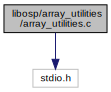
\includegraphics[width=184pt]{array__utilities_8c__incl}
\end{center}
\end{figure}
\subsection*{Functions}
\begin{DoxyCompactItemize}
\item 
void \mbox{\hyperlink{array__utilities_8c_a64e51535b38f41ede085ef4a25fa28cd}{array\+\_\+flip}} (float $\ast$arr, int len)
\item 
float \mbox{\hyperlink{array__utilities_8c_a66f72f5e1e55efe67aed2e7d25f620cf}{array\+\_\+sum}} (float $\ast$arr, size\+\_\+t len)
\begin{DoxyCompactList}\small\item\em Function to calculate the sum of an array. \end{DoxyCompactList}\item 
float \mbox{\hyperlink{array__utilities_8c_a0374927fa364e07942cfe0afd8eb3bf7}{array\+\_\+dot\+\_\+product}} (float $\ast$in1, float $\ast$in2, size\+\_\+t len)
\begin{DoxyCompactList}\small\item\em Function to calculate the dot-\/product of two 1-\/D vectors/arrays. \end{DoxyCompactList}\item 
void \mbox{\hyperlink{array__utilities_8c_ac5e150940a31a2aace5bc977dfed62e7}{array\+\_\+right\+\_\+shift}} (float $\ast$arr, size\+\_\+t len)
\begin{DoxyCompactList}\small\item\em Function to right shift an array by one place. Left most value will be replaced by zero. \end{DoxyCompactList}\item 
void \mbox{\hyperlink{array__utilities_8c_ae9c0f53e57eba1f9b68b3b98035c7104}{array\+\_\+multiply\+\_\+const}} (float $\ast$arr, float constant, size\+\_\+t len)
\begin{DoxyCompactList}\small\item\em Function to multiply each element of an array by a scalar constant. \end{DoxyCompactList}\item 
void \mbox{\hyperlink{array__utilities_8c_ac5021e5ce6e8fbcdefd4ec345304363e}{array\+\_\+add\+\_\+const}} (float $\ast$arr, float constant, size\+\_\+t len)
\begin{DoxyCompactList}\small\item\em Function to add a scalar constant to each element of an array. \end{DoxyCompactList}\item 
void \mbox{\hyperlink{array__utilities_8c_ac37c2fb5baed3b9e871704d40bd565fe}{array\+\_\+add\+\_\+array}} (float $\ast$in1, float $\ast$in2, size\+\_\+t len)
\begin{DoxyCompactList}\small\item\em Function to do element wise addition of two arrays. \end{DoxyCompactList}\item 
void \mbox{\hyperlink{array__utilities_8c_a545e6953015959c5a450bd64b82df25b}{array\+\_\+subtract\+\_\+array}} (float $\ast$in1, float $\ast$in2, size\+\_\+t len)
\begin{DoxyCompactList}\small\item\em Function to do element wise subtraction of two arrays. \end{DoxyCompactList}\item 
void \mbox{\hyperlink{array__utilities_8c_a9f327998fca4f21185d509294f1a8da4}{array\+\_\+element\+\_\+multiply\+\_\+array}} (float $\ast$in1, float $\ast$in2, size\+\_\+t len)
\begin{DoxyCompactList}\small\item\em Function to do element wise multiplication of two arrays. \end{DoxyCompactList}\item 
void \mbox{\hyperlink{array__utilities_8c_a0589a77beeb385b229b27849ac01eebd}{array\+\_\+element\+\_\+divide\+\_\+array}} (float $\ast$in1, float $\ast$in2, size\+\_\+t len)
\begin{DoxyCompactList}\small\item\em Function to do element wise division of two arrays. \end{DoxyCompactList}\item 
float \mbox{\hyperlink{array__utilities_8c_a64d2006c296282872c8a3282db12d82c}{array\+\_\+min}} (float $\ast$arr, size\+\_\+t len)
\begin{DoxyCompactList}\small\item\em Function to return the minimum of the elements of an array. \end{DoxyCompactList}\item 
float \mbox{\hyperlink{array__utilities_8c_abd95915e71cdf97c66dd2092aed740df}{array\+\_\+mean}} (float $\ast$arr, size\+\_\+t len)
\begin{DoxyCompactList}\small\item\em Function to calculate the mean of the elements of an array. \end{DoxyCompactList}\item 
void \mbox{\hyperlink{array__utilities_8c_a93dbc84e75a7252ad994e9f79777dee7}{array\+\_\+square}} (float $\ast$in, float $\ast$out, size\+\_\+t len)
\begin{DoxyCompactList}\small\item\em Function to populate the output array with square of the elements of an input array. \end{DoxyCompactList}\item 
float \mbox{\hyperlink{array__utilities_8c_a909d668ad88464159d6b2ad5574e06be}{array\+\_\+mean\+\_\+square}} (float $\ast$arr, size\+\_\+t len)
\begin{DoxyCompactList}\small\item\em Function to calculate the mean square of the elements of an array. \end{DoxyCompactList}\item 
void \mbox{\hyperlink{array__utilities_8c_acad9b9e456a0f3a81dab2671224f150c}{memcpy\+\_\+f}} (float $\ast$dst, float $\ast$src, size\+\_\+t len)
\begin{DoxyCompactList}\small\item\em Function to copy an array from source to destination. \end{DoxyCompactList}\item 
void \mbox{\hyperlink{array__utilities_8c_ad1f8261eef0b72711c198bdc73fb934d}{array\+\_\+print}} (const char $\ast$str, float $\ast$arr, size\+\_\+t len)
\begin{DoxyCompactList}\small\item\em Function to print an array for debugging. \end{DoxyCompactList}\end{DoxyCompactItemize}


\subsection{Function Documentation}
\mbox{\Hypertarget{array__utilities_8c_ac37c2fb5baed3b9e871704d40bd565fe}\label{array__utilities_8c_ac37c2fb5baed3b9e871704d40bd565fe}} 
\index{array\+\_\+utilities.\+c@{array\+\_\+utilities.\+c}!array\+\_\+add\+\_\+array@{array\+\_\+add\+\_\+array}}
\index{array\+\_\+add\+\_\+array@{array\+\_\+add\+\_\+array}!array\+\_\+utilities.\+c@{array\+\_\+utilities.\+c}}
\subsubsection{\texorpdfstring{array\+\_\+add\+\_\+array()}{array\_add\_array()}}
{\footnotesize\ttfamily void array\+\_\+add\+\_\+array (\begin{DoxyParamCaption}\item[{float $\ast$}]{in1,  }\item[{float $\ast$}]{in2,  }\item[{size\+\_\+t}]{len }\end{DoxyParamCaption})}



Function to do element wise addition of two arrays. 


\begin{DoxyParams}{Parameters}
{\em in1} & Pointer to the first array \\
\hline
{\em in2} & Pointer to the second array \\
\hline
{\em len} & Length of the arrays \\
\hline
\end{DoxyParams}
\begin{DoxyWarning}{Warning}
Assumes both the arrays are of same length and takes only one length parameter 
\end{DoxyWarning}
\mbox{\Hypertarget{array__utilities_8c_ac5021e5ce6e8fbcdefd4ec345304363e}\label{array__utilities_8c_ac5021e5ce6e8fbcdefd4ec345304363e}} 
\index{array\+\_\+utilities.\+c@{array\+\_\+utilities.\+c}!array\+\_\+add\+\_\+const@{array\+\_\+add\+\_\+const}}
\index{array\+\_\+add\+\_\+const@{array\+\_\+add\+\_\+const}!array\+\_\+utilities.\+c@{array\+\_\+utilities.\+c}}
\subsubsection{\texorpdfstring{array\+\_\+add\+\_\+const()}{array\_add\_const()}}
{\footnotesize\ttfamily void array\+\_\+add\+\_\+const (\begin{DoxyParamCaption}\item[{float $\ast$}]{arr,  }\item[{float}]{constant,  }\item[{size\+\_\+t}]{len }\end{DoxyParamCaption})}



Function to add a scalar constant to each element of an array. 


\begin{DoxyParams}{Parameters}
{\em arr} & Pointer to the array \\
\hline
{\em constant} & The constant scalar adder \\
\hline
{\em len} & Length of the array \\
\hline
\end{DoxyParams}
\mbox{\Hypertarget{array__utilities_8c_a0374927fa364e07942cfe0afd8eb3bf7}\label{array__utilities_8c_a0374927fa364e07942cfe0afd8eb3bf7}} 
\index{array\+\_\+utilities.\+c@{array\+\_\+utilities.\+c}!array\+\_\+dot\+\_\+product@{array\+\_\+dot\+\_\+product}}
\index{array\+\_\+dot\+\_\+product@{array\+\_\+dot\+\_\+product}!array\+\_\+utilities.\+c@{array\+\_\+utilities.\+c}}
\subsubsection{\texorpdfstring{array\+\_\+dot\+\_\+product()}{array\_dot\_product()}}
{\footnotesize\ttfamily float array\+\_\+dot\+\_\+product (\begin{DoxyParamCaption}\item[{float $\ast$}]{in1,  }\item[{float $\ast$}]{in2,  }\item[{size\+\_\+t}]{len }\end{DoxyParamCaption})}



Function to calculate the dot-\/product of two 1-\/D vectors/arrays. 


\begin{DoxyParams}{Parameters}
{\em in1} & Pointer to the first vector \\
\hline
{\em in2} & Pointer to the second vector \\
\hline
{\em len} & Length of the vectors \\
\hline
\end{DoxyParams}
\begin{DoxyReturn}{Returns}
Dot product (inner product) of the two vectors 
\end{DoxyReturn}
\begin{DoxyWarning}{Warning}
Assumes both the vectors are of same length and takes only one length parameter 
\end{DoxyWarning}
\mbox{\Hypertarget{array__utilities_8c_a0589a77beeb385b229b27849ac01eebd}\label{array__utilities_8c_a0589a77beeb385b229b27849ac01eebd}} 
\index{array\+\_\+utilities.\+c@{array\+\_\+utilities.\+c}!array\+\_\+element\+\_\+divide\+\_\+array@{array\+\_\+element\+\_\+divide\+\_\+array}}
\index{array\+\_\+element\+\_\+divide\+\_\+array@{array\+\_\+element\+\_\+divide\+\_\+array}!array\+\_\+utilities.\+c@{array\+\_\+utilities.\+c}}
\subsubsection{\texorpdfstring{array\+\_\+element\+\_\+divide\+\_\+array()}{array\_element\_divide\_array()}}
{\footnotesize\ttfamily void array\+\_\+element\+\_\+divide\+\_\+array (\begin{DoxyParamCaption}\item[{float $\ast$}]{in1,  }\item[{float $\ast$}]{in2,  }\item[{size\+\_\+t}]{len }\end{DoxyParamCaption})}



Function to do element wise division of two arrays. 


\begin{DoxyParams}{Parameters}
{\em in1} & Pointer to the first array \\
\hline
{\em in2} & Pointer to the second array \\
\hline
{\em len} & Length of the arrays \\
\hline
\end{DoxyParams}
\begin{DoxyWarning}{Warning}
Assumes both the arrays are of same length and takes only one length parameter 
\end{DoxyWarning}
\mbox{\Hypertarget{array__utilities_8c_a9f327998fca4f21185d509294f1a8da4}\label{array__utilities_8c_a9f327998fca4f21185d509294f1a8da4}} 
\index{array\+\_\+utilities.\+c@{array\+\_\+utilities.\+c}!array\+\_\+element\+\_\+multiply\+\_\+array@{array\+\_\+element\+\_\+multiply\+\_\+array}}
\index{array\+\_\+element\+\_\+multiply\+\_\+array@{array\+\_\+element\+\_\+multiply\+\_\+array}!array\+\_\+utilities.\+c@{array\+\_\+utilities.\+c}}
\subsubsection{\texorpdfstring{array\+\_\+element\+\_\+multiply\+\_\+array()}{array\_element\_multiply\_array()}}
{\footnotesize\ttfamily void array\+\_\+element\+\_\+multiply\+\_\+array (\begin{DoxyParamCaption}\item[{float $\ast$}]{in1,  }\item[{float $\ast$}]{in2,  }\item[{size\+\_\+t}]{len }\end{DoxyParamCaption})}



Function to do element wise multiplication of two arrays. 


\begin{DoxyParams}{Parameters}
{\em in1} & Pointer to the first array \\
\hline
{\em in2} & Pointer to the second array \\
\hline
{\em len} & Length of the arrays \\
\hline
\end{DoxyParams}
\begin{DoxyWarning}{Warning}
Assumes both the arrays are of same length and takes only one length parameter 
\end{DoxyWarning}
\mbox{\Hypertarget{array__utilities_8c_a64e51535b38f41ede085ef4a25fa28cd}\label{array__utilities_8c_a64e51535b38f41ede085ef4a25fa28cd}} 
\index{array\+\_\+utilities.\+c@{array\+\_\+utilities.\+c}!array\+\_\+flip@{array\+\_\+flip}}
\index{array\+\_\+flip@{array\+\_\+flip}!array\+\_\+utilities.\+c@{array\+\_\+utilities.\+c}}
\subsubsection{\texorpdfstring{array\+\_\+flip()}{array\_flip()}}
{\footnotesize\ttfamily void array\+\_\+flip (\begin{DoxyParamCaption}\item[{float $\ast$}]{arr,  }\item[{int}]{len }\end{DoxyParamCaption})}

\mbox{\Hypertarget{array__utilities_8c_abd95915e71cdf97c66dd2092aed740df}\label{array__utilities_8c_abd95915e71cdf97c66dd2092aed740df}} 
\index{array\+\_\+utilities.\+c@{array\+\_\+utilities.\+c}!array\+\_\+mean@{array\+\_\+mean}}
\index{array\+\_\+mean@{array\+\_\+mean}!array\+\_\+utilities.\+c@{array\+\_\+utilities.\+c}}
\subsubsection{\texorpdfstring{array\+\_\+mean()}{array\_mean()}}
{\footnotesize\ttfamily float array\+\_\+mean (\begin{DoxyParamCaption}\item[{float $\ast$}]{arr,  }\item[{size\+\_\+t}]{len }\end{DoxyParamCaption})}



Function to calculate the mean of the elements of an array. 


\begin{DoxyParams}{Parameters}
{\em arr} & Pointer to the array \\
\hline
{\em len} & Length of the array \\
\hline
\end{DoxyParams}
\begin{DoxyReturn}{Returns}
Mean of the array elements 
\end{DoxyReturn}
\mbox{\Hypertarget{array__utilities_8c_a909d668ad88464159d6b2ad5574e06be}\label{array__utilities_8c_a909d668ad88464159d6b2ad5574e06be}} 
\index{array\+\_\+utilities.\+c@{array\+\_\+utilities.\+c}!array\+\_\+mean\+\_\+square@{array\+\_\+mean\+\_\+square}}
\index{array\+\_\+mean\+\_\+square@{array\+\_\+mean\+\_\+square}!array\+\_\+utilities.\+c@{array\+\_\+utilities.\+c}}
\subsubsection{\texorpdfstring{array\+\_\+mean\+\_\+square()}{array\_mean\_square()}}
{\footnotesize\ttfamily float array\+\_\+mean\+\_\+square (\begin{DoxyParamCaption}\item[{float $\ast$}]{arr,  }\item[{size\+\_\+t}]{len }\end{DoxyParamCaption})}



Function to calculate the mean square of the elements of an array. 


\begin{DoxyParams}{Parameters}
{\em arr} & Pointer to the array \\
\hline
{\em len} & Length of the array \\
\hline
\end{DoxyParams}
\begin{DoxyReturn}{Returns}
Mean square of the array elements 
\end{DoxyReturn}
\mbox{\Hypertarget{array__utilities_8c_a64d2006c296282872c8a3282db12d82c}\label{array__utilities_8c_a64d2006c296282872c8a3282db12d82c}} 
\index{array\+\_\+utilities.\+c@{array\+\_\+utilities.\+c}!array\+\_\+min@{array\+\_\+min}}
\index{array\+\_\+min@{array\+\_\+min}!array\+\_\+utilities.\+c@{array\+\_\+utilities.\+c}}
\subsubsection{\texorpdfstring{array\+\_\+min()}{array\_min()}}
{\footnotesize\ttfamily float array\+\_\+min (\begin{DoxyParamCaption}\item[{float $\ast$}]{arr,  }\item[{size\+\_\+t}]{len }\end{DoxyParamCaption})}



Function to return the minimum of the elements of an array. 


\begin{DoxyParams}{Parameters}
{\em arr} & Pointer to the array \\
\hline
{\em len} & Length of the array \\
\hline
\end{DoxyParams}
\begin{DoxyReturn}{Returns}
Minimum of the array elements 
\end{DoxyReturn}
\mbox{\Hypertarget{array__utilities_8c_ae9c0f53e57eba1f9b68b3b98035c7104}\label{array__utilities_8c_ae9c0f53e57eba1f9b68b3b98035c7104}} 
\index{array\+\_\+utilities.\+c@{array\+\_\+utilities.\+c}!array\+\_\+multiply\+\_\+const@{array\+\_\+multiply\+\_\+const}}
\index{array\+\_\+multiply\+\_\+const@{array\+\_\+multiply\+\_\+const}!array\+\_\+utilities.\+c@{array\+\_\+utilities.\+c}}
\subsubsection{\texorpdfstring{array\+\_\+multiply\+\_\+const()}{array\_multiply\_const()}}
{\footnotesize\ttfamily void array\+\_\+multiply\+\_\+const (\begin{DoxyParamCaption}\item[{float $\ast$}]{arr,  }\item[{float}]{constant,  }\item[{size\+\_\+t}]{len }\end{DoxyParamCaption})}



Function to multiply each element of an array by a scalar constant. 


\begin{DoxyParams}{Parameters}
{\em arr} & Pointer to the array \\
\hline
{\em constant} & The constant scalar multiplier \\
\hline
{\em len} & Length of the array \\
\hline
\end{DoxyParams}
\mbox{\Hypertarget{array__utilities_8c_ad1f8261eef0b72711c198bdc73fb934d}\label{array__utilities_8c_ad1f8261eef0b72711c198bdc73fb934d}} 
\index{array\+\_\+utilities.\+c@{array\+\_\+utilities.\+c}!array\+\_\+print@{array\+\_\+print}}
\index{array\+\_\+print@{array\+\_\+print}!array\+\_\+utilities.\+c@{array\+\_\+utilities.\+c}}
\subsubsection{\texorpdfstring{array\+\_\+print()}{array\_print()}}
{\footnotesize\ttfamily void array\+\_\+print (\begin{DoxyParamCaption}\item[{const char $\ast$}]{str,  }\item[{float $\ast$}]{arr,  }\item[{size\+\_\+t}]{len }\end{DoxyParamCaption})}



Function to print an array for debugging. 


\begin{DoxyParams}{Parameters}
{\em str} & String to use for debugging \\
\hline
{\em arr} & Pointer to the array \\
\hline
{\em len} & Length of the array \\
\hline
\end{DoxyParams}
\mbox{\Hypertarget{array__utilities_8c_ac5e150940a31a2aace5bc977dfed62e7}\label{array__utilities_8c_ac5e150940a31a2aace5bc977dfed62e7}} 
\index{array\+\_\+utilities.\+c@{array\+\_\+utilities.\+c}!array\+\_\+right\+\_\+shift@{array\+\_\+right\+\_\+shift}}
\index{array\+\_\+right\+\_\+shift@{array\+\_\+right\+\_\+shift}!array\+\_\+utilities.\+c@{array\+\_\+utilities.\+c}}
\subsubsection{\texorpdfstring{array\+\_\+right\+\_\+shift()}{array\_right\_shift()}}
{\footnotesize\ttfamily void array\+\_\+right\+\_\+shift (\begin{DoxyParamCaption}\item[{float $\ast$}]{arr,  }\item[{size\+\_\+t}]{len }\end{DoxyParamCaption})}



Function to right shift an array by one place. Left most value will be replaced by zero. 


\begin{DoxyParams}{Parameters}
{\em arr} & Pointer to the array \\
\hline
{\em len} & Length of the array \\
\hline
\end{DoxyParams}
\mbox{\Hypertarget{array__utilities_8c_a93dbc84e75a7252ad994e9f79777dee7}\label{array__utilities_8c_a93dbc84e75a7252ad994e9f79777dee7}} 
\index{array\+\_\+utilities.\+c@{array\+\_\+utilities.\+c}!array\+\_\+square@{array\+\_\+square}}
\index{array\+\_\+square@{array\+\_\+square}!array\+\_\+utilities.\+c@{array\+\_\+utilities.\+c}}
\subsubsection{\texorpdfstring{array\+\_\+square()}{array\_square()}}
{\footnotesize\ttfamily void array\+\_\+square (\begin{DoxyParamCaption}\item[{float $\ast$}]{in,  }\item[{float $\ast$}]{out,  }\item[{size\+\_\+t}]{len }\end{DoxyParamCaption})}



Function to populate the output array with square of the elements of an input array. 


\begin{DoxyParams}{Parameters}
{\em in} & Pointer to the input array \\
\hline
{\em out} & Pointer to the output array \\
\hline
{\em len} & Length of the arrays \\
\hline
\end{DoxyParams}
\begin{DoxyWarning}{Warning}
Assumes that output array already has memory allocated to it 
\end{DoxyWarning}
\mbox{\Hypertarget{array__utilities_8c_a545e6953015959c5a450bd64b82df25b}\label{array__utilities_8c_a545e6953015959c5a450bd64b82df25b}} 
\index{array\+\_\+utilities.\+c@{array\+\_\+utilities.\+c}!array\+\_\+subtract\+\_\+array@{array\+\_\+subtract\+\_\+array}}
\index{array\+\_\+subtract\+\_\+array@{array\+\_\+subtract\+\_\+array}!array\+\_\+utilities.\+c@{array\+\_\+utilities.\+c}}
\subsubsection{\texorpdfstring{array\+\_\+subtract\+\_\+array()}{array\_subtract\_array()}}
{\footnotesize\ttfamily void array\+\_\+subtract\+\_\+array (\begin{DoxyParamCaption}\item[{float $\ast$}]{in1,  }\item[{float $\ast$}]{in2,  }\item[{size\+\_\+t}]{len }\end{DoxyParamCaption})}



Function to do element wise subtraction of two arrays. 


\begin{DoxyParams}{Parameters}
{\em in1} & Pointer to the first array \\
\hline
{\em in2} & Pointer to the second array \\
\hline
{\em len} & Length of the arrays \\
\hline
\end{DoxyParams}
\begin{DoxyWarning}{Warning}
Assumes both the arrays are of same length and takes only one length parameter 
\end{DoxyWarning}
\mbox{\Hypertarget{array__utilities_8c_a66f72f5e1e55efe67aed2e7d25f620cf}\label{array__utilities_8c_a66f72f5e1e55efe67aed2e7d25f620cf}} 
\index{array\+\_\+utilities.\+c@{array\+\_\+utilities.\+c}!array\+\_\+sum@{array\+\_\+sum}}
\index{array\+\_\+sum@{array\+\_\+sum}!array\+\_\+utilities.\+c@{array\+\_\+utilities.\+c}}
\subsubsection{\texorpdfstring{array\+\_\+sum()}{array\_sum()}}
{\footnotesize\ttfamily float array\+\_\+sum (\begin{DoxyParamCaption}\item[{float $\ast$}]{arr,  }\item[{size\+\_\+t}]{len }\end{DoxyParamCaption})}



Function to calculate the sum of an array. 


\begin{DoxyParams}{Parameters}
{\em arr} & Pointer to the array \\
\hline
{\em len} & Length of the array \\
\hline
\end{DoxyParams}
\begin{DoxyReturn}{Returns}
Sum of the array 
\end{DoxyReturn}
\mbox{\Hypertarget{array__utilities_8c_acad9b9e456a0f3a81dab2671224f150c}\label{array__utilities_8c_acad9b9e456a0f3a81dab2671224f150c}} 
\index{array\+\_\+utilities.\+c@{array\+\_\+utilities.\+c}!memcpy\+\_\+f@{memcpy\+\_\+f}}
\index{memcpy\+\_\+f@{memcpy\+\_\+f}!array\+\_\+utilities.\+c@{array\+\_\+utilities.\+c}}
\subsubsection{\texorpdfstring{memcpy\+\_\+f()}{memcpy\_f()}}
{\footnotesize\ttfamily void memcpy\+\_\+f (\begin{DoxyParamCaption}\item[{float $\ast$}]{dst,  }\item[{float $\ast$}]{src,  }\item[{size\+\_\+t}]{len }\end{DoxyParamCaption})}



Function to copy an array from source to destination. 


\begin{DoxyParams}{Parameters}
{\em dst} & Pointer to the destination array \\
\hline
{\em src} & Pointer to the source array \\
\hline
{\em len} & Length of the arrays \\
\hline
\end{DoxyParams}
\begin{DoxyWarning}{Warning}
Assumes that destination array already has memory allocated to it 
\end{DoxyWarning}

\input{array__utilities_8h}
\hypertarget{beam__forming_8c}{}\section{libosp/beam\+\_\+forming/beam\+\_\+forming.c File Reference}
\label{beam__forming_8c}\index{libosp/beam\+\_\+forming/beam\+\_\+forming.\+c@{libosp/beam\+\_\+forming/beam\+\_\+forming.\+c}}
{\ttfamily \#include $<$stdlib.\+h$>$}\newline
{\ttfamily \#include $<$math.\+h$>$}\newline
{\ttfamily \#include \char`\"{}beam\+\_\+forming.\+h\char`\"{}}\newline
{\ttfamily \#include \char`\"{}delay\+\_\+line.\+h\char`\"{}}\newline
Include dependency graph for beam\+\_\+forming.\+c\+:\nopagebreak
\begin{figure}[H]
\begin{center}
\leavevmode
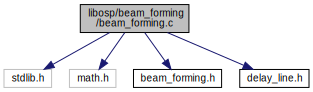
\includegraphics[width=350pt]{beam__forming_8c__incl}
\end{center}
\end{figure}
\subsection*{Data Structures}
\begin{DoxyCompactItemize}
\item 
struct \mbox{\hyperlink{structbeam__form__t}{beam\+\_\+form\+\_\+t}}
\begin{DoxyCompactList}\small\item\em data structure containing relevant beam-\/forming fields \end{DoxyCompactList}\end{DoxyCompactItemize}
\subsection*{Macros}
\begin{DoxyCompactItemize}
\item 
\#define \mbox{\hyperlink{beam__forming_8c_a9d41d147039787c25d6631b276ab4330}{D\+I\+S\+T\+A\+N\+CE}}~0.\+1
\begin{DoxyCompactList}\small\item\em Distance between front and rear microphones in meters. \end{DoxyCompactList}\item 
\#define \mbox{\hyperlink{beam__forming_8c_ac9f9f9d25bbf964365102f1ef77d359e}{S\+P\+E\+E\+D\+\_\+\+O\+F\+\_\+\+S\+O\+U\+ND}}~340.\+29
\begin{DoxyCompactList}\small\item\em Speed of sound in meters/second. \end{DoxyCompactList}\end{DoxyCompactItemize}
\subsection*{Functions}
\begin{DoxyCompactItemize}
\item 
\mbox{\hyperlink{beam__forming_8h_a9199414346374516a0281f253490d683}{Beam\+\_\+\+Form}} \mbox{\hyperlink{beam__forming_8c_af1500dbad6977e67b77ddcb693399b4c}{beam\+\_\+form\+\_\+init}} (float beta, float gain, float sample\+\_\+rate)
\begin{DoxyCompactList}\small\item\em Initialization function for the beam forming data struct. \end{DoxyCompactList}\item 
void \mbox{\hyperlink{beam__forming_8c_ae641e306d725c5ee093d5179e49ec252}{beam\+\_\+form\+\_\+proc}} (\mbox{\hyperlink{beam__forming_8h_a9199414346374516a0281f253490d683}{Beam\+\_\+\+Form}} beam\+\_\+form, float $\ast$in\+\_\+front, float $\ast$in\+\_\+rear, float $\ast$output, int len)
\begin{DoxyCompactList}\small\item\em Takes in two channel inputs, and attempts to use beamforming to provide directed output The in\+\_\+front, in\+\_\+rear, and output arrays must be allocated so that they are len samples long. \end{DoxyCompactList}\item 
void \mbox{\hyperlink{beam__forming_8c_aa555d80ffa96de7c2221a70a24f04fe4}{beam\+\_\+form\+\_\+destroy}} (\mbox{\hyperlink{beam__forming_8h_a9199414346374516a0281f253490d683}{Beam\+\_\+\+Form}} beam\+\_\+form)
\begin{DoxyCompactList}\small\item\em Closes and frees the beam\+\_\+form instance. \end{DoxyCompactList}\end{DoxyCompactItemize}


\subsection{Macro Definition Documentation}
\mbox{\Hypertarget{beam__forming_8c_a9d41d147039787c25d6631b276ab4330}\label{beam__forming_8c_a9d41d147039787c25d6631b276ab4330}} 
\index{beam\+\_\+forming.\+c@{beam\+\_\+forming.\+c}!D\+I\+S\+T\+A\+N\+CE@{D\+I\+S\+T\+A\+N\+CE}}
\index{D\+I\+S\+T\+A\+N\+CE@{D\+I\+S\+T\+A\+N\+CE}!beam\+\_\+forming.\+c@{beam\+\_\+forming.\+c}}
\subsubsection{\texorpdfstring{D\+I\+S\+T\+A\+N\+CE}{DISTANCE}}
{\footnotesize\ttfamily \#define D\+I\+S\+T\+A\+N\+CE~0.\+1}



Distance between front and rear microphones in meters. 

\mbox{\Hypertarget{beam__forming_8c_ac9f9f9d25bbf964365102f1ef77d359e}\label{beam__forming_8c_ac9f9f9d25bbf964365102f1ef77d359e}} 
\index{beam\+\_\+forming.\+c@{beam\+\_\+forming.\+c}!S\+P\+E\+E\+D\+\_\+\+O\+F\+\_\+\+S\+O\+U\+ND@{S\+P\+E\+E\+D\+\_\+\+O\+F\+\_\+\+S\+O\+U\+ND}}
\index{S\+P\+E\+E\+D\+\_\+\+O\+F\+\_\+\+S\+O\+U\+ND@{S\+P\+E\+E\+D\+\_\+\+O\+F\+\_\+\+S\+O\+U\+ND}!beam\+\_\+forming.\+c@{beam\+\_\+forming.\+c}}
\subsubsection{\texorpdfstring{S\+P\+E\+E\+D\+\_\+\+O\+F\+\_\+\+S\+O\+U\+ND}{SPEED\_OF\_SOUND}}
{\footnotesize\ttfamily \#define S\+P\+E\+E\+D\+\_\+\+O\+F\+\_\+\+S\+O\+U\+ND~340.\+29}



Speed of sound in meters/second. 



\subsection{Function Documentation}
\mbox{\Hypertarget{beam__forming_8c_aa555d80ffa96de7c2221a70a24f04fe4}\label{beam__forming_8c_aa555d80ffa96de7c2221a70a24f04fe4}} 
\index{beam\+\_\+forming.\+c@{beam\+\_\+forming.\+c}!beam\+\_\+form\+\_\+destroy@{beam\+\_\+form\+\_\+destroy}}
\index{beam\+\_\+form\+\_\+destroy@{beam\+\_\+form\+\_\+destroy}!beam\+\_\+forming.\+c@{beam\+\_\+forming.\+c}}
\subsubsection{\texorpdfstring{beam\+\_\+form\+\_\+destroy()}{beam\_form\_destroy()}}
{\footnotesize\ttfamily void beam\+\_\+form\+\_\+destroy (\begin{DoxyParamCaption}\item[{\mbox{\hyperlink{beam__forming_8h_a9199414346374516a0281f253490d683}{Beam\+\_\+\+Form}}}]{beam\+\_\+form }\end{DoxyParamCaption})}



Closes and frees the beam\+\_\+form instance. 

\begin{DoxySeeAlso}{See also}
\mbox{\hyperlink{structbeam__form__t}{beam\+\_\+form\+\_\+t}} 
\end{DoxySeeAlso}

\begin{DoxyParams}{Parameters}
{\em beam\+\_\+form} & The instance of the Beam\+\_\+\+Form variable that was returned from beam\+\_\+form\+\_\+init \\
\hline
\end{DoxyParams}
\mbox{\Hypertarget{beam__forming_8c_af1500dbad6977e67b77ddcb693399b4c}\label{beam__forming_8c_af1500dbad6977e67b77ddcb693399b4c}} 
\index{beam\+\_\+forming.\+c@{beam\+\_\+forming.\+c}!beam\+\_\+form\+\_\+init@{beam\+\_\+form\+\_\+init}}
\index{beam\+\_\+form\+\_\+init@{beam\+\_\+form\+\_\+init}!beam\+\_\+forming.\+c@{beam\+\_\+forming.\+c}}
\subsubsection{\texorpdfstring{beam\+\_\+form\+\_\+init()}{beam\_form\_init()}}
{\footnotesize\ttfamily \mbox{\hyperlink{beam__forming_8h_a9199414346374516a0281f253490d683}{Beam\+\_\+\+Form}} beam\+\_\+form\+\_\+init (\begin{DoxyParamCaption}\item[{float}]{beta,  }\item[{float}]{gain,  }\item[{float}]{sample\+\_\+rate }\end{DoxyParamCaption})}



Initialization function for the beam forming data struct. 

\begin{DoxySeeAlso}{See also}
\mbox{\hyperlink{structbeam__form__t}{beam\+\_\+form\+\_\+t}} 
\end{DoxySeeAlso}

\begin{DoxyParams}{Parameters}
{\em beta} & beta value \\
\hline
{\em gain} & gain value \\
\hline
{\em sample\+\_\+rate} & Sample rate set by audio drivers. Used in calculation of angle \\
\hline
\end{DoxyParams}
\begin{DoxyReturn}{Returns}
Returns the allocated instance of the beamforming data structure (\char`\"{}object\char`\"{}) 
\end{DoxyReturn}
\mbox{\Hypertarget{beam__forming_8c_ae641e306d725c5ee093d5179e49ec252}\label{beam__forming_8c_ae641e306d725c5ee093d5179e49ec252}} 
\index{beam\+\_\+forming.\+c@{beam\+\_\+forming.\+c}!beam\+\_\+form\+\_\+proc@{beam\+\_\+form\+\_\+proc}}
\index{beam\+\_\+form\+\_\+proc@{beam\+\_\+form\+\_\+proc}!beam\+\_\+forming.\+c@{beam\+\_\+forming.\+c}}
\subsubsection{\texorpdfstring{beam\+\_\+form\+\_\+proc()}{beam\_form\_proc()}}
{\footnotesize\ttfamily void beam\+\_\+form\+\_\+proc (\begin{DoxyParamCaption}\item[{\mbox{\hyperlink{beam__forming_8h_a9199414346374516a0281f253490d683}{Beam\+\_\+\+Form}}}]{beam\+\_\+form,  }\item[{float $\ast$}]{in\+\_\+front,  }\item[{float $\ast$}]{in\+\_\+rear,  }\item[{float $\ast$}]{output,  }\item[{int}]{len }\end{DoxyParamCaption})}



Takes in two channel inputs, and attempts to use beamforming to provide directed output The in\+\_\+front, in\+\_\+rear, and output arrays must be allocated so that they are len samples long. 

\begin{DoxySeeAlso}{See also}
\mbox{\hyperlink{structbeam__form__t}{beam\+\_\+form\+\_\+t}} 
\end{DoxySeeAlso}

\begin{DoxyParams}{Parameters}
{\em beam\+\_\+form} & The instance of the Beam\+\_\+\+Form variable that was returned from beam\+\_\+form\+\_\+init \\
\hline
{\em in\+\_\+front} & Float array of the input samples from the \char`\"{}front\char`\"{} mic that are len floats long \\
\hline
{\em in\+\_\+rear} & Float array of the samples from the \char`\"{}rear\char`\"{} mic that are len floats long \\
\hline
{\em output} & Float array containing the processed samples that are len floats long \\
\hline
{\em len} & The length of the input \\
\hline
\end{DoxyParams}

\hypertarget{beam__forming_8h}{}\section{libosp/beam\+\_\+forming/beam\+\_\+forming.h File Reference}
\label{beam__forming_8h}\index{libosp/beam\+\_\+forming/beam\+\_\+forming.\+h@{libosp/beam\+\_\+forming/beam\+\_\+forming.\+h}}
This graph shows which files directly or indirectly include this file\+:\nopagebreak
\begin{figure}[H]
\begin{center}
\leavevmode
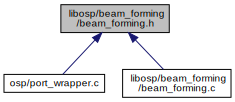
\includegraphics[width=308pt]{beam__forming_8h__dep__incl}
\end{center}
\end{figure}
\subsection*{Typedefs}
\begin{DoxyCompactItemize}
\item 
typedef struct \mbox{\hyperlink{structbeam__form__t}{beam\+\_\+form\+\_\+t}} $\ast$ \mbox{\hyperlink{beam__forming_8h_a9199414346374516a0281f253490d683}{Beam\+\_\+\+Form}}
\end{DoxyCompactItemize}
\subsection*{Functions}
\begin{DoxyCompactItemize}
\item 
\mbox{\hyperlink{beam__forming_8h_a9199414346374516a0281f253490d683}{Beam\+\_\+\+Form}} \mbox{\hyperlink{beam__forming_8h_af1500dbad6977e67b77ddcb693399b4c}{beam\+\_\+form\+\_\+init}} (float beta, float gain, float sample\+\_\+rate)
\begin{DoxyCompactList}\small\item\em Initialization function for the beam forming data struct. \end{DoxyCompactList}\item 
void \mbox{\hyperlink{beam__forming_8h_ae641e306d725c5ee093d5179e49ec252}{beam\+\_\+form\+\_\+proc}} (\mbox{\hyperlink{beam__forming_8h_a9199414346374516a0281f253490d683}{Beam\+\_\+\+Form}} beam\+\_\+form, float $\ast$in\+\_\+front, float $\ast$in\+\_\+rear, float $\ast$output, int len)
\begin{DoxyCompactList}\small\item\em Takes in two channel inputs, and attempts to use beamforming to provide directed output The in\+\_\+front, in\+\_\+rear, and output arrays must be allocated so that they are len samples long. \end{DoxyCompactList}\item 
void \mbox{\hyperlink{beam__forming_8h_aa555d80ffa96de7c2221a70a24f04fe4}{beam\+\_\+form\+\_\+destroy}} (\mbox{\hyperlink{beam__forming_8h_a9199414346374516a0281f253490d683}{Beam\+\_\+\+Form}} beam\+\_\+form)
\begin{DoxyCompactList}\small\item\em Closes and frees the beam\+\_\+form instance. \end{DoxyCompactList}\end{DoxyCompactItemize}


\subsection{Typedef Documentation}
\mbox{\Hypertarget{beam__forming_8h_a9199414346374516a0281f253490d683}\label{beam__forming_8h_a9199414346374516a0281f253490d683}} 
\index{beam\+\_\+forming.\+h@{beam\+\_\+forming.\+h}!Beam\+\_\+\+Form@{Beam\+\_\+\+Form}}
\index{Beam\+\_\+\+Form@{Beam\+\_\+\+Form}!beam\+\_\+forming.\+h@{beam\+\_\+forming.\+h}}
\subsubsection{\texorpdfstring{Beam\+\_\+\+Form}{Beam\_Form}}
{\footnotesize\ttfamily typedef struct \mbox{\hyperlink{structbeam__form__t}{beam\+\_\+form\+\_\+t}}$\ast$ \mbox{\hyperlink{beam__forming_8h_a9199414346374516a0281f253490d683}{Beam\+\_\+\+Form}}}



\subsection{Function Documentation}
\mbox{\Hypertarget{beam__forming_8h_aa555d80ffa96de7c2221a70a24f04fe4}\label{beam__forming_8h_aa555d80ffa96de7c2221a70a24f04fe4}} 
\index{beam\+\_\+forming.\+h@{beam\+\_\+forming.\+h}!beam\+\_\+form\+\_\+destroy@{beam\+\_\+form\+\_\+destroy}}
\index{beam\+\_\+form\+\_\+destroy@{beam\+\_\+form\+\_\+destroy}!beam\+\_\+forming.\+h@{beam\+\_\+forming.\+h}}
\subsubsection{\texorpdfstring{beam\+\_\+form\+\_\+destroy()}{beam\_form\_destroy()}}
{\footnotesize\ttfamily void beam\+\_\+form\+\_\+destroy (\begin{DoxyParamCaption}\item[{\mbox{\hyperlink{beam__forming_8h_a9199414346374516a0281f253490d683}{Beam\+\_\+\+Form}}}]{beam\+\_\+form }\end{DoxyParamCaption})}



Closes and frees the beam\+\_\+form instance. 

\begin{DoxySeeAlso}{See also}
\mbox{\hyperlink{structbeam__form__t}{beam\+\_\+form\+\_\+t}} 
\end{DoxySeeAlso}

\begin{DoxyParams}{Parameters}
{\em beam\+\_\+form} & The instance of the Beam\+\_\+\+Form variable that was returned from beam\+\_\+form\+\_\+init \\
\hline
\end{DoxyParams}
\mbox{\Hypertarget{beam__forming_8h_af1500dbad6977e67b77ddcb693399b4c}\label{beam__forming_8h_af1500dbad6977e67b77ddcb693399b4c}} 
\index{beam\+\_\+forming.\+h@{beam\+\_\+forming.\+h}!beam\+\_\+form\+\_\+init@{beam\+\_\+form\+\_\+init}}
\index{beam\+\_\+form\+\_\+init@{beam\+\_\+form\+\_\+init}!beam\+\_\+forming.\+h@{beam\+\_\+forming.\+h}}
\subsubsection{\texorpdfstring{beam\+\_\+form\+\_\+init()}{beam\_form\_init()}}
{\footnotesize\ttfamily \mbox{\hyperlink{beam__forming_8h_a9199414346374516a0281f253490d683}{Beam\+\_\+\+Form}} beam\+\_\+form\+\_\+init (\begin{DoxyParamCaption}\item[{float}]{beta,  }\item[{float}]{gain,  }\item[{float}]{sample\+\_\+rate }\end{DoxyParamCaption})}



Initialization function for the beam forming data struct. 

\begin{DoxySeeAlso}{See also}
\mbox{\hyperlink{structbeam__form__t}{beam\+\_\+form\+\_\+t}} 
\end{DoxySeeAlso}

\begin{DoxyParams}{Parameters}
{\em beta} & beta value \\
\hline
{\em gain} & gain value \\
\hline
{\em sample\+\_\+rate} & Sample rate set by audio drivers. Used in calculation of angle \\
\hline
\end{DoxyParams}
\begin{DoxyReturn}{Returns}
Returns the allocated instance of the beamforming data structure (\char`\"{}object\char`\"{}) 
\end{DoxyReturn}
\mbox{\Hypertarget{beam__forming_8h_ae641e306d725c5ee093d5179e49ec252}\label{beam__forming_8h_ae641e306d725c5ee093d5179e49ec252}} 
\index{beam\+\_\+forming.\+h@{beam\+\_\+forming.\+h}!beam\+\_\+form\+\_\+proc@{beam\+\_\+form\+\_\+proc}}
\index{beam\+\_\+form\+\_\+proc@{beam\+\_\+form\+\_\+proc}!beam\+\_\+forming.\+h@{beam\+\_\+forming.\+h}}
\subsubsection{\texorpdfstring{beam\+\_\+form\+\_\+proc()}{beam\_form\_proc()}}
{\footnotesize\ttfamily void beam\+\_\+form\+\_\+proc (\begin{DoxyParamCaption}\item[{\mbox{\hyperlink{beam__forming_8h_a9199414346374516a0281f253490d683}{Beam\+\_\+\+Form}}}]{beam\+\_\+form,  }\item[{float $\ast$}]{in\+\_\+front,  }\item[{float $\ast$}]{in\+\_\+rear,  }\item[{float $\ast$}]{output,  }\item[{int}]{len }\end{DoxyParamCaption})}



Takes in two channel inputs, and attempts to use beamforming to provide directed output The in\+\_\+front, in\+\_\+rear, and output arrays must be allocated so that they are len samples long. 

\begin{DoxySeeAlso}{See also}
\mbox{\hyperlink{structbeam__form__t}{beam\+\_\+form\+\_\+t}} 
\end{DoxySeeAlso}

\begin{DoxyParams}{Parameters}
{\em beam\+\_\+form} & The instance of the Beam\+\_\+\+Form variable that was returned from beam\+\_\+form\+\_\+init \\
\hline
{\em in\+\_\+front} & Float array of the input samples from the \char`\"{}front\char`\"{} mic that are len floats long \\
\hline
{\em in\+\_\+rear} & Float array of the samples from the \char`\"{}rear\char`\"{} mic that are len floats long \\
\hline
{\em output} & Float array containing the processed samples that are len floats long \\
\hline
{\em len} & The length of the input \\
\hline
\end{DoxyParams}

\hypertarget{delay__line_8c}{}\section{libosp/beam\+\_\+forming/delay\+\_\+line.c File Reference}
\label{delay__line_8c}\index{libosp/beam\+\_\+forming/delay\+\_\+line.\+c@{libosp/beam\+\_\+forming/delay\+\_\+line.\+c}}
{\ttfamily \#include \char`\"{}delay\+\_\+line.\+h\char`\"{}}\newline
{\ttfamily \#include $<$stdlib.\+h$>$}\newline
{\ttfamily \#include $<$string.\+h$>$}\newline
{\ttfamily \#include $<$math.\+h$>$}\newline
Include dependency graph for delay\+\_\+line.\+c\+:\nopagebreak
\begin{figure}[H]
\begin{center}
\leavevmode
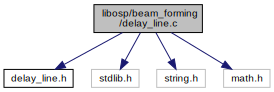
\includegraphics[width=347pt]{delay__line_8c__incl}
\end{center}
\end{figure}
\subsection*{Data Structures}
\begin{DoxyCompactItemize}
\item 
struct \mbox{\hyperlink{structdelay__line__t}{delay\+\_\+line\+\_\+t}}
\begin{DoxyCompactList}\small\item\em Data structure that contains delay\+\_\+line information. \end{DoxyCompactList}\end{DoxyCompactItemize}
\subsection*{Functions}
\begin{DoxyCompactItemize}
\item 
\mbox{\hyperlink{delay__line_8h_aa62b49f8bfee0c3a174896c9b446d68d}{Delay\+\_\+\+Line}} \mbox{\hyperlink{delay__line_8c_a7e4b8dbf2a223a4014061763f039ed07}{delay\+\_\+line\+\_\+init}} (unsigned int delay)
\begin{DoxyCompactList}\small\item\em Initializes Delay Line structure. \end{DoxyCompactList}\item 
float \mbox{\hyperlink{delay__line_8c_a0e9e86a07f0e0b2dfa0826bde02983e8}{delay\+\_\+line\+\_\+tick}} (\mbox{\hyperlink{delay__line_8h_aa62b49f8bfee0c3a174896c9b446d68d}{Delay\+\_\+\+Line}} del\+\_\+line, float input\+\_\+sample)
\begin{DoxyCompactList}\small\item\em Returns an output sample that has been delayed by a set number When you call delay\+\_\+line\+\_\+tick with a sample, you are putting a sample into its internal circular buffer, and you are getting a sample that has previously been put onto its circular buffer N samples/ticks ago (where N is the delay parameter in delay\+\_\+line\+\_\+init). \end{DoxyCompactList}\item 
int \mbox{\hyperlink{delay__line_8c_a4010a68b463ce7bc8fe47ffd59b917b4}{delay\+\_\+line\+\_\+free}} (\mbox{\hyperlink{delay__line_8h_aa62b49f8bfee0c3a174896c9b446d68d}{Delay\+\_\+\+Line}} del\+\_\+line)
\begin{DoxyCompactList}\small\item\em Frees the Delay\+\_\+\+Line data structure. \end{DoxyCompactList}\item 
int \mbox{\hyperlink{delay__line_8c_a0c4320f88c683a623950f95a844a1466}{delay\+\_\+line\+\_\+flush}} (\mbox{\hyperlink{delay__line_8h_aa62b49f8bfee0c3a174896c9b446d68d}{Delay\+\_\+\+Line}} del\+\_\+line)
\begin{DoxyCompactList}\small\item\em Flushes internal circular buffer that contains previous samples put on by calls to delay\+\_\+line\+\_\+tick. \end{DoxyCompactList}\end{DoxyCompactItemize}


\subsection{Function Documentation}
\mbox{\Hypertarget{delay__line_8c_a0c4320f88c683a623950f95a844a1466}\label{delay__line_8c_a0c4320f88c683a623950f95a844a1466}} 
\index{delay\+\_\+line.\+c@{delay\+\_\+line.\+c}!delay\+\_\+line\+\_\+flush@{delay\+\_\+line\+\_\+flush}}
\index{delay\+\_\+line\+\_\+flush@{delay\+\_\+line\+\_\+flush}!delay\+\_\+line.\+c@{delay\+\_\+line.\+c}}
\subsubsection{\texorpdfstring{delay\+\_\+line\+\_\+flush()}{delay\_line\_flush()}}
{\footnotesize\ttfamily int delay\+\_\+line\+\_\+flush (\begin{DoxyParamCaption}\item[{\mbox{\hyperlink{delay__line_8h_aa62b49f8bfee0c3a174896c9b446d68d}{Delay\+\_\+\+Line}}}]{del\+\_\+line }\end{DoxyParamCaption})}



Flushes internal circular buffer that contains previous samples put on by calls to delay\+\_\+line\+\_\+tick. 


\begin{DoxyParams}{Parameters}
{\em del\+\_\+line} & The data structure containing delay\+\_\+line details \\
\hline
\end{DoxyParams}
\begin{DoxyReturn}{Returns}
0 on success, -\/1 otherwise. Need to fix this 
\end{DoxyReturn}
\mbox{\Hypertarget{delay__line_8c_a4010a68b463ce7bc8fe47ffd59b917b4}\label{delay__line_8c_a4010a68b463ce7bc8fe47ffd59b917b4}} 
\index{delay\+\_\+line.\+c@{delay\+\_\+line.\+c}!delay\+\_\+line\+\_\+free@{delay\+\_\+line\+\_\+free}}
\index{delay\+\_\+line\+\_\+free@{delay\+\_\+line\+\_\+free}!delay\+\_\+line.\+c@{delay\+\_\+line.\+c}}
\subsubsection{\texorpdfstring{delay\+\_\+line\+\_\+free()}{delay\_line\_free()}}
{\footnotesize\ttfamily int delay\+\_\+line\+\_\+free (\begin{DoxyParamCaption}\item[{\mbox{\hyperlink{delay__line_8h_aa62b49f8bfee0c3a174896c9b446d68d}{Delay\+\_\+\+Line}}}]{del\+\_\+line }\end{DoxyParamCaption})}



Frees the Delay\+\_\+\+Line data structure. 


\begin{DoxyParams}{Parameters}
{\em del\+\_\+line} & Delay\+\_\+\+Line data structure to be freed \\
\hline
\end{DoxyParams}
\begin{DoxyReturn}{Returns}
0 on success, -\/1 otherwise 
\end{DoxyReturn}
\mbox{\Hypertarget{delay__line_8c_a7e4b8dbf2a223a4014061763f039ed07}\label{delay__line_8c_a7e4b8dbf2a223a4014061763f039ed07}} 
\index{delay\+\_\+line.\+c@{delay\+\_\+line.\+c}!delay\+\_\+line\+\_\+init@{delay\+\_\+line\+\_\+init}}
\index{delay\+\_\+line\+\_\+init@{delay\+\_\+line\+\_\+init}!delay\+\_\+line.\+c@{delay\+\_\+line.\+c}}
\subsubsection{\texorpdfstring{delay\+\_\+line\+\_\+init()}{delay\_line\_init()}}
{\footnotesize\ttfamily \mbox{\hyperlink{delay__line_8h_aa62b49f8bfee0c3a174896c9b446d68d}{Delay\+\_\+\+Line}} delay\+\_\+line\+\_\+init (\begin{DoxyParamCaption}\item[{unsigned int}]{delay }\end{DoxyParamCaption})}



Initializes Delay Line structure. 

\begin{DoxySeeAlso}{See also}
\mbox{\hyperlink{delay__line_8h_a0e9e86a07f0e0b2dfa0826bde02983e8}{delay\+\_\+line\+\_\+tick}} 
\end{DoxySeeAlso}

\begin{DoxyParams}{Parameters}
{\em delay} & The number of samples to delay when calling delay\+\_\+line\+\_\+tick \\
\hline
\end{DoxyParams}
\begin{DoxyReturn}{Returns}
Returns the Delay\+\_\+\+Line data structure 
\end{DoxyReturn}
\mbox{\Hypertarget{delay__line_8c_a0e9e86a07f0e0b2dfa0826bde02983e8}\label{delay__line_8c_a0e9e86a07f0e0b2dfa0826bde02983e8}} 
\index{delay\+\_\+line.\+c@{delay\+\_\+line.\+c}!delay\+\_\+line\+\_\+tick@{delay\+\_\+line\+\_\+tick}}
\index{delay\+\_\+line\+\_\+tick@{delay\+\_\+line\+\_\+tick}!delay\+\_\+line.\+c@{delay\+\_\+line.\+c}}
\subsubsection{\texorpdfstring{delay\+\_\+line\+\_\+tick()}{delay\_line\_tick()}}
{\footnotesize\ttfamily float delay\+\_\+line\+\_\+tick (\begin{DoxyParamCaption}\item[{\mbox{\hyperlink{delay__line_8h_aa62b49f8bfee0c3a174896c9b446d68d}{Delay\+\_\+\+Line}}}]{del\+\_\+line,  }\item[{float}]{input\+\_\+sample }\end{DoxyParamCaption})}



Returns an output sample that has been delayed by a set number When you call delay\+\_\+line\+\_\+tick with a sample, you are putting a sample into its internal circular buffer, and you are getting a sample that has previously been put onto its circular buffer N samples/ticks ago (where N is the delay parameter in delay\+\_\+line\+\_\+init). 

For example, if you set the delay\+\_\+line\+\_\+init with a delay of 4 samples, the input and output of delay\+\_\+line\+\_\+tick are shown below, where each row represents calling the delay\+\_\+line\+\_\+tick function In Out 1 0 1 0 1 0 1 0 0 1 0 1 0 1 0 1 0 0 0 0 ...


\begin{DoxyParams}{Parameters}
{\em del\+\_\+line} & The Delay\+\_\+\+Line struct returned from delay\+\_\+line\+\_\+init \\
\hline
{\em input\+\_\+sample} & The input sample that will be returned N ticks in the future\\
\hline
\end{DoxyParams}
\begin{DoxyReturn}{Returns}
A sample that was previously passed into delay\+\_\+line\+\_\+tick N ticks in the past 
\end{DoxyReturn}

\hypertarget{delay__line_8h}{}\section{libosp/beam\+\_\+forming/delay\+\_\+line.h File Reference}
\label{delay__line_8h}\index{libosp/beam\+\_\+forming/delay\+\_\+line.\+h@{libosp/beam\+\_\+forming/delay\+\_\+line.\+h}}
This graph shows which files directly or indirectly include this file\+:\nopagebreak
\begin{figure}[H]
\begin{center}
\leavevmode
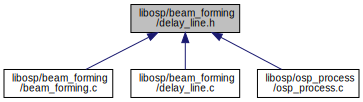
\includegraphics[width=350pt]{delay__line_8h__dep__incl}
\end{center}
\end{figure}
\subsection*{Typedefs}
\begin{DoxyCompactItemize}
\item 
typedef struct \mbox{\hyperlink{structdelay__line__t}{delay\+\_\+line\+\_\+t}} $\ast$ \mbox{\hyperlink{delay__line_8h_aa62b49f8bfee0c3a174896c9b446d68d}{Delay\+\_\+\+Line}}
\end{DoxyCompactItemize}
\subsection*{Functions}
\begin{DoxyCompactItemize}
\item 
\mbox{\hyperlink{delay__line_8h_aa62b49f8bfee0c3a174896c9b446d68d}{Delay\+\_\+\+Line}} \mbox{\hyperlink{delay__line_8h_a7e4b8dbf2a223a4014061763f039ed07}{delay\+\_\+line\+\_\+init}} (unsigned int delay)
\begin{DoxyCompactList}\small\item\em Initializes Delay Line structure. \end{DoxyCompactList}\item 
float \mbox{\hyperlink{delay__line_8h_a0e9e86a07f0e0b2dfa0826bde02983e8}{delay\+\_\+line\+\_\+tick}} (\mbox{\hyperlink{delay__line_8h_aa62b49f8bfee0c3a174896c9b446d68d}{Delay\+\_\+\+Line}} del\+\_\+line, float input\+\_\+sample)
\begin{DoxyCompactList}\small\item\em Returns an output sample that has been delayed by a set number When you call delay\+\_\+line\+\_\+tick with a sample, you are putting a sample into its internal circular buffer, and you are getting a sample that has previously been put onto its circular buffer N samples/ticks ago (where N is the delay parameter in delay\+\_\+line\+\_\+init). \end{DoxyCompactList}\item 
int \mbox{\hyperlink{delay__line_8h_a4010a68b463ce7bc8fe47ffd59b917b4}{delay\+\_\+line\+\_\+free}} (\mbox{\hyperlink{delay__line_8h_aa62b49f8bfee0c3a174896c9b446d68d}{Delay\+\_\+\+Line}} del\+\_\+line)
\begin{DoxyCompactList}\small\item\em Frees the Delay\+\_\+\+Line data structure. \end{DoxyCompactList}\item 
int \mbox{\hyperlink{delay__line_8h_a0c4320f88c683a623950f95a844a1466}{delay\+\_\+line\+\_\+flush}} (\mbox{\hyperlink{delay__line_8h_aa62b49f8bfee0c3a174896c9b446d68d}{Delay\+\_\+\+Line}} del\+\_\+line)
\begin{DoxyCompactList}\small\item\em Flushes internal circular buffer that contains previous samples put on by calls to delay\+\_\+line\+\_\+tick. \end{DoxyCompactList}\end{DoxyCompactItemize}


\subsection{Typedef Documentation}
\mbox{\Hypertarget{delay__line_8h_aa62b49f8bfee0c3a174896c9b446d68d}\label{delay__line_8h_aa62b49f8bfee0c3a174896c9b446d68d}} 
\index{delay\+\_\+line.\+h@{delay\+\_\+line.\+h}!Delay\+\_\+\+Line@{Delay\+\_\+\+Line}}
\index{Delay\+\_\+\+Line@{Delay\+\_\+\+Line}!delay\+\_\+line.\+h@{delay\+\_\+line.\+h}}
\subsubsection{\texorpdfstring{Delay\+\_\+\+Line}{Delay\_Line}}
{\footnotesize\ttfamily typedef struct \mbox{\hyperlink{structdelay__line__t}{delay\+\_\+line\+\_\+t}}$\ast$ \mbox{\hyperlink{delay__line_8h_aa62b49f8bfee0c3a174896c9b446d68d}{Delay\+\_\+\+Line}}}



\subsection{Function Documentation}
\mbox{\Hypertarget{delay__line_8h_a0c4320f88c683a623950f95a844a1466}\label{delay__line_8h_a0c4320f88c683a623950f95a844a1466}} 
\index{delay\+\_\+line.\+h@{delay\+\_\+line.\+h}!delay\+\_\+line\+\_\+flush@{delay\+\_\+line\+\_\+flush}}
\index{delay\+\_\+line\+\_\+flush@{delay\+\_\+line\+\_\+flush}!delay\+\_\+line.\+h@{delay\+\_\+line.\+h}}
\subsubsection{\texorpdfstring{delay\+\_\+line\+\_\+flush()}{delay\_line\_flush()}}
{\footnotesize\ttfamily int delay\+\_\+line\+\_\+flush (\begin{DoxyParamCaption}\item[{\mbox{\hyperlink{delay__line_8h_aa62b49f8bfee0c3a174896c9b446d68d}{Delay\+\_\+\+Line}}}]{del\+\_\+line }\end{DoxyParamCaption})}



Flushes internal circular buffer that contains previous samples put on by calls to delay\+\_\+line\+\_\+tick. 


\begin{DoxyParams}{Parameters}
{\em del\+\_\+line} & The data structure containing delay\+\_\+line details \\
\hline
\end{DoxyParams}
\begin{DoxyReturn}{Returns}
0 on success, -\/1 otherwise. Need to fix this 
\end{DoxyReturn}
\mbox{\Hypertarget{delay__line_8h_a4010a68b463ce7bc8fe47ffd59b917b4}\label{delay__line_8h_a4010a68b463ce7bc8fe47ffd59b917b4}} 
\index{delay\+\_\+line.\+h@{delay\+\_\+line.\+h}!delay\+\_\+line\+\_\+free@{delay\+\_\+line\+\_\+free}}
\index{delay\+\_\+line\+\_\+free@{delay\+\_\+line\+\_\+free}!delay\+\_\+line.\+h@{delay\+\_\+line.\+h}}
\subsubsection{\texorpdfstring{delay\+\_\+line\+\_\+free()}{delay\_line\_free()}}
{\footnotesize\ttfamily int delay\+\_\+line\+\_\+free (\begin{DoxyParamCaption}\item[{\mbox{\hyperlink{delay__line_8h_aa62b49f8bfee0c3a174896c9b446d68d}{Delay\+\_\+\+Line}}}]{del\+\_\+line }\end{DoxyParamCaption})}



Frees the Delay\+\_\+\+Line data structure. 


\begin{DoxyParams}{Parameters}
{\em del\+\_\+line} & Delay\+\_\+\+Line data structure to be freed \\
\hline
\end{DoxyParams}
\begin{DoxyReturn}{Returns}
0 on success, -\/1 otherwise 
\end{DoxyReturn}
\mbox{\Hypertarget{delay__line_8h_a7e4b8dbf2a223a4014061763f039ed07}\label{delay__line_8h_a7e4b8dbf2a223a4014061763f039ed07}} 
\index{delay\+\_\+line.\+h@{delay\+\_\+line.\+h}!delay\+\_\+line\+\_\+init@{delay\+\_\+line\+\_\+init}}
\index{delay\+\_\+line\+\_\+init@{delay\+\_\+line\+\_\+init}!delay\+\_\+line.\+h@{delay\+\_\+line.\+h}}
\subsubsection{\texorpdfstring{delay\+\_\+line\+\_\+init()}{delay\_line\_init()}}
{\footnotesize\ttfamily \mbox{\hyperlink{delay__line_8h_aa62b49f8bfee0c3a174896c9b446d68d}{Delay\+\_\+\+Line}} delay\+\_\+line\+\_\+init (\begin{DoxyParamCaption}\item[{unsigned int}]{delay }\end{DoxyParamCaption})}



Initializes Delay Line structure. 

\begin{DoxySeeAlso}{See also}
\mbox{\hyperlink{delay__line_8h_a0e9e86a07f0e0b2dfa0826bde02983e8}{delay\+\_\+line\+\_\+tick}} 
\end{DoxySeeAlso}

\begin{DoxyParams}{Parameters}
{\em delay} & The number of samples to delay when calling delay\+\_\+line\+\_\+tick \\
\hline
\end{DoxyParams}
\begin{DoxyReturn}{Returns}
Returns the Delay\+\_\+\+Line data structure 
\end{DoxyReturn}
\mbox{\Hypertarget{delay__line_8h_a0e9e86a07f0e0b2dfa0826bde02983e8}\label{delay__line_8h_a0e9e86a07f0e0b2dfa0826bde02983e8}} 
\index{delay\+\_\+line.\+h@{delay\+\_\+line.\+h}!delay\+\_\+line\+\_\+tick@{delay\+\_\+line\+\_\+tick}}
\index{delay\+\_\+line\+\_\+tick@{delay\+\_\+line\+\_\+tick}!delay\+\_\+line.\+h@{delay\+\_\+line.\+h}}
\subsubsection{\texorpdfstring{delay\+\_\+line\+\_\+tick()}{delay\_line\_tick()}}
{\footnotesize\ttfamily float delay\+\_\+line\+\_\+tick (\begin{DoxyParamCaption}\item[{\mbox{\hyperlink{delay__line_8h_aa62b49f8bfee0c3a174896c9b446d68d}{Delay\+\_\+\+Line}}}]{del\+\_\+line,  }\item[{float}]{input\+\_\+sample }\end{DoxyParamCaption})}



Returns an output sample that has been delayed by a set number When you call delay\+\_\+line\+\_\+tick with a sample, you are putting a sample into its internal circular buffer, and you are getting a sample that has previously been put onto its circular buffer N samples/ticks ago (where N is the delay parameter in delay\+\_\+line\+\_\+init). 

For example, if you set the delay\+\_\+line\+\_\+init with a delay of 4 samples, the input and output of delay\+\_\+line\+\_\+tick are shown below, where each row represents calling the delay\+\_\+line\+\_\+tick function In Out 1 0 1 0 1 0 1 0 0 1 0 1 0 1 0 1 0 0 0 0 ...


\begin{DoxyParams}{Parameters}
{\em del\+\_\+line} & The Delay\+\_\+\+Line struct returned from delay\+\_\+line\+\_\+init \\
\hline
{\em input\+\_\+sample} & The input sample that will be returned N ticks in the future\\
\hline
\end{DoxyParams}
\begin{DoxyReturn}{Returns}
A sample that was previously passed into delay\+\_\+line\+\_\+tick N ticks in the past 
\end{DoxyReturn}

\hypertarget{constants_8h}{}\section{libosp/common/constants.h File Reference}
\label{constants_8h}\index{libosp/common/constants.\+h@{libosp/common/constants.\+h}}
This graph shows which files directly or indirectly include this file\+:\nopagebreak
\begin{figure}[H]
\begin{center}
\leavevmode
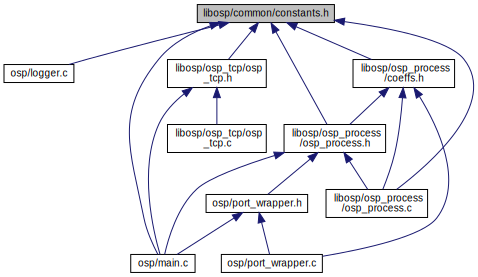
\includegraphics[width=350pt]{constants_8h__dep__incl}
\end{center}
\end{figure}
\subsection*{Data Structures}
\begin{DoxyCompactItemize}
\item 
struct \mbox{\hyperlink{structpa__aux__data__t}{pa\+\_\+aux\+\_\+data\+\_\+t}}
\begin{DoxyCompactList}\small\item\em Struct that contains misc data passed to Port\+Audio. \end{DoxyCompactList}\item 
struct \mbox{\hyperlink{structosp__user__data__t}{osp\+\_\+user\+\_\+data\+\_\+t}}
\begin{DoxyCompactList}\small\item\em general data structure shared between client and C application \end{DoxyCompactList}\item 
struct \mbox{\hyperlink{structpa__user__data__t}{pa\+\_\+user\+\_\+data\+\_\+t}}
\begin{DoxyCompactList}\small\item\em The data structure passed to Port\+Audio. \end{DoxyCompactList}\end{DoxyCompactItemize}
\subsection*{Macros}
\begin{DoxyCompactItemize}
\item 
\#define \mbox{\hyperlink{constants_8h_af9b1b2ba12857a4bf11289dac8c5462d}{F\+R\+A\+M\+E\+\_\+\+S\+I\+ZE}}~32
\begin{DoxyCompactList}\small\item\em Contains general, commonly used data structures and constants. \end{DoxyCompactList}\item 
\#define \mbox{\hyperlink{constants_8h_a1c6d5de492ac61ad29aec7aa9a436bbf}{V\+E\+R\+S\+I\+ON}}~2
\begin{DoxyCompactList}\small\item\em This is the C version for keeping the networking of packets between the. \end{DoxyCompactList}\item 
\#define \mbox{\hyperlink{constants_8h_a19441d7b9be72492ed93a440085e53be}{N\+U\+M\+\_\+\+B\+A\+N\+DS}}~6
\begin{DoxyCompactList}\small\item\em Number of Sub-\/\+Bands. \end{DoxyCompactList}\item 
\#define \mbox{\hyperlink{constants_8h_a452c7c8774a73a5b8cbd4563653a21af}{B\+A\+N\+D\+\_\+\+F\+I\+L\+T\+\_\+\+L\+EN}}~193
\begin{DoxyCompactList}\small\item\em Sub-\/\+Band filter tap length. \end{DoxyCompactList}\item 
\#define \mbox{\hyperlink{constants_8h_a22ad4850ff1e8ce8e185cf535c32c26e}{R\+E\+S\+A\+M\+P\+\_\+96\+\_\+32\+\_\+\+T\+A\+PS}}~25
\begin{DoxyCompactList}\small\item\em Number of taps for decimation filter in resampler.\+c. \end{DoxyCompactList}\item 
\#define \mbox{\hyperlink{constants_8h_af1c688c1719e08f8a604305465450147}{R\+E\+S\+A\+M\+P\+\_\+32\+\_\+96\+\_\+\+T\+A\+PS}}~25
\begin{DoxyCompactList}\small\item\em Number of taps for interpolation filter in resampler.\+c. \end{DoxyCompactList}\item 
\#define \mbox{\hyperlink{constants_8h_a9b84aa2154cd9ca7cb142e726240a5d7}{R\+E\+S\+A\+M\+P\+\_\+48\+\_\+32\+\_\+\+T\+A\+PS}}~25
\begin{DoxyCompactList}\small\item\em Number of taps for decimation filter in resampler.\+c for 48 to 32 k\+Hz. \end{DoxyCompactList}\item 
\#define \mbox{\hyperlink{constants_8h_acb1026ec40e93e9b7791eeea149b8e7c}{R\+E\+S\+A\+M\+P\+\_\+32\+\_\+48\+\_\+\+T\+A\+PS}}~25
\begin{DoxyCompactList}\small\item\em Number of taps for interpolation filter in resampler.\+c for 32 to 48 k\+Hz. \end{DoxyCompactList}\item 
\#define \mbox{\hyperlink{constants_8h_aac913071759241f612b525eb18b88c21}{S\+Y\+N\+T\+H\+E\+T\+I\+C\+\_\+\+T\+A\+P\+\_\+\+L\+EN}}~525
\begin{DoxyCompactList}\small\item\em Synthetic feedback filter tap length. \end{DoxyCompactList}\item 
\#define \mbox{\hyperlink{constants_8h_aa6fad7476783d6554d6960266fc9710e}{D\+\_\+\+A\+T\+T\+A\+C\+K\+\_\+\+T\+I\+ME}}~5
\begin{DoxyCompactList}\small\item\em Attack time in msec. \end{DoxyCompactList}\item 
\#define \mbox{\hyperlink{constants_8h_a23e7303689b2693b49c214078260ff07}{D\+\_\+\+R\+E\+L\+E\+A\+S\+E\+\_\+\+T\+I\+ME}}~20
\begin{DoxyCompactList}\small\item\em Release time in msec. \end{DoxyCompactList}\item 
\#define \mbox{\hyperlink{constants_8h_a2b99a14a394089869b4ddfd90770b744}{D\+\_\+\+P\+D\+\_\+\+S\+A\+M\+P\+\_\+\+R\+A\+TE}}~32000
\begin{DoxyCompactList}\small\item\em Sample rate that M\+HA is operating at. \end{DoxyCompactList}\item 
\#define \mbox{\hyperlink{constants_8h_ac0c3f81bc6d1bff60a7151fd357c9553}{D\+\_\+\+K\+N\+E\+E\+\_\+\+L\+OW}}~45
\begin{DoxyCompactList}\small\item\em Lower kneepoint in dB S\+PL. Using the same value for all the bands. \end{DoxyCompactList}\item 
\#define \mbox{\hyperlink{constants_8h_a1d3c631a46d2c01ca8c30f8b1950baec}{D\+\_\+\+K\+N\+E\+E\+\_\+\+H\+I\+GH}}~100
\begin{DoxyCompactList}\small\item\em Upper kneepoint in dB S\+PL. Using the same value for all the bands. \end{DoxyCompactList}\item 
\#define \mbox{\hyperlink{constants_8h_ab7d9d3d6b6e2a1e24cf9a4045e7a2112}{A\+F\+C\+\_\+\+F\+I\+L\+T\+E\+R\+\_\+\+T\+A\+P\+\_\+\+F\+I\+L\+E\+\_\+L}}~\char`\"{}./afc\+\_\+filter\+\_\+taps\+\_\+l.\+bin\char`\"{}
\begin{DoxyCompactList}\small\item\em A\+FC filter initialization taps for left channel. \end{DoxyCompactList}\item 
\#define \mbox{\hyperlink{constants_8h_a8de8458e1ba37e0233dce701a8b4fd89}{A\+F\+C\+\_\+\+F\+I\+L\+T\+E\+R\+\_\+\+T\+A\+P\+\_\+\+F\+I\+L\+E\+\_\+R}}~\char`\"{}./afc\+\_\+filter\+\_\+taps\+\_\+r.\+bin\char`\"{}
\begin{DoxyCompactList}\small\item\em A\+FC filter initialization taps for right channel. \end{DoxyCompactList}\item 
\#define \mbox{\hyperlink{constants_8h_ac4ec0a338c1546cbff3dfd95a3eac2de}{C\+U\+R\+R\+E\+N\+T\+\_\+\+V\+E\+R\+S\+I\+ON}}~1
\begin{DoxyCompactList}\small\item\em Version number of the application. Required to match the version with Android app. \end{DoxyCompactList}\end{DoxyCompactItemize}
\subsection*{Typedefs}
\begin{DoxyCompactItemize}
\item 
typedef struct \mbox{\hyperlink{structpa__aux__data__t}{pa\+\_\+aux\+\_\+data\+\_\+t}} \mbox{\hyperlink{constants_8h_add46628e302aedde68d37aea654eda24}{pa\+\_\+aux\+\_\+data}}
\begin{DoxyCompactList}\small\item\em Struct that contains misc data passed to Port\+Audio. \end{DoxyCompactList}\item 
typedef struct \mbox{\hyperlink{structosp__user__data__t}{osp\+\_\+user\+\_\+data\+\_\+t}} \mbox{\hyperlink{constants_8h_a2d1d78531fe12807c3852488556d5a4b}{osp\+\_\+user\+\_\+data}}
\begin{DoxyCompactList}\small\item\em general data structure shared between client and C application \end{DoxyCompactList}\item 
typedef struct \mbox{\hyperlink{structpa__user__data__t}{pa\+\_\+user\+\_\+data\+\_\+t}} \mbox{\hyperlink{constants_8h_aba6e2261d5c6ef36dedb5b45ba0fc4ae}{pa\+\_\+user\+\_\+data}}
\begin{DoxyCompactList}\small\item\em The data structure passed to Port\+Audio. \end{DoxyCompactList}\end{DoxyCompactItemize}


\subsection{Macro Definition Documentation}
\mbox{\Hypertarget{constants_8h_ab7d9d3d6b6e2a1e24cf9a4045e7a2112}\label{constants_8h_ab7d9d3d6b6e2a1e24cf9a4045e7a2112}} 
\index{constants.\+h@{constants.\+h}!A\+F\+C\+\_\+\+F\+I\+L\+T\+E\+R\+\_\+\+T\+A\+P\+\_\+\+F\+I\+L\+E\+\_\+L@{A\+F\+C\+\_\+\+F\+I\+L\+T\+E\+R\+\_\+\+T\+A\+P\+\_\+\+F\+I\+L\+E\+\_\+L}}
\index{A\+F\+C\+\_\+\+F\+I\+L\+T\+E\+R\+\_\+\+T\+A\+P\+\_\+\+F\+I\+L\+E\+\_\+L@{A\+F\+C\+\_\+\+F\+I\+L\+T\+E\+R\+\_\+\+T\+A\+P\+\_\+\+F\+I\+L\+E\+\_\+L}!constants.\+h@{constants.\+h}}
\subsubsection{\texorpdfstring{A\+F\+C\+\_\+\+F\+I\+L\+T\+E\+R\+\_\+\+T\+A\+P\+\_\+\+F\+I\+L\+E\+\_\+L}{AFC\_FILTER\_TAP\_FILE\_L}}
{\footnotesize\ttfamily \#define A\+F\+C\+\_\+\+F\+I\+L\+T\+E\+R\+\_\+\+T\+A\+P\+\_\+\+F\+I\+L\+E\+\_\+L~\char`\"{}./afc\+\_\+filter\+\_\+taps\+\_\+l.\+bin\char`\"{}}



A\+FC filter initialization taps for left channel. 

\mbox{\Hypertarget{constants_8h_a8de8458e1ba37e0233dce701a8b4fd89}\label{constants_8h_a8de8458e1ba37e0233dce701a8b4fd89}} 
\index{constants.\+h@{constants.\+h}!A\+F\+C\+\_\+\+F\+I\+L\+T\+E\+R\+\_\+\+T\+A\+P\+\_\+\+F\+I\+L\+E\+\_\+R@{A\+F\+C\+\_\+\+F\+I\+L\+T\+E\+R\+\_\+\+T\+A\+P\+\_\+\+F\+I\+L\+E\+\_\+R}}
\index{A\+F\+C\+\_\+\+F\+I\+L\+T\+E\+R\+\_\+\+T\+A\+P\+\_\+\+F\+I\+L\+E\+\_\+R@{A\+F\+C\+\_\+\+F\+I\+L\+T\+E\+R\+\_\+\+T\+A\+P\+\_\+\+F\+I\+L\+E\+\_\+R}!constants.\+h@{constants.\+h}}
\subsubsection{\texorpdfstring{A\+F\+C\+\_\+\+F\+I\+L\+T\+E\+R\+\_\+\+T\+A\+P\+\_\+\+F\+I\+L\+E\+\_\+R}{AFC\_FILTER\_TAP\_FILE\_R}}
{\footnotesize\ttfamily \#define A\+F\+C\+\_\+\+F\+I\+L\+T\+E\+R\+\_\+\+T\+A\+P\+\_\+\+F\+I\+L\+E\+\_\+R~\char`\"{}./afc\+\_\+filter\+\_\+taps\+\_\+r.\+bin\char`\"{}}



A\+FC filter initialization taps for right channel. 

\mbox{\Hypertarget{constants_8h_a452c7c8774a73a5b8cbd4563653a21af}\label{constants_8h_a452c7c8774a73a5b8cbd4563653a21af}} 
\index{constants.\+h@{constants.\+h}!B\+A\+N\+D\+\_\+\+F\+I\+L\+T\+\_\+\+L\+EN@{B\+A\+N\+D\+\_\+\+F\+I\+L\+T\+\_\+\+L\+EN}}
\index{B\+A\+N\+D\+\_\+\+F\+I\+L\+T\+\_\+\+L\+EN@{B\+A\+N\+D\+\_\+\+F\+I\+L\+T\+\_\+\+L\+EN}!constants.\+h@{constants.\+h}}
\subsubsection{\texorpdfstring{B\+A\+N\+D\+\_\+\+F\+I\+L\+T\+\_\+\+L\+EN}{BAND\_FILT\_LEN}}
{\footnotesize\ttfamily \#define B\+A\+N\+D\+\_\+\+F\+I\+L\+T\+\_\+\+L\+EN~193}



Sub-\/\+Band filter tap length. 

\mbox{\Hypertarget{constants_8h_ac4ec0a338c1546cbff3dfd95a3eac2de}\label{constants_8h_ac4ec0a338c1546cbff3dfd95a3eac2de}} 
\index{constants.\+h@{constants.\+h}!C\+U\+R\+R\+E\+N\+T\+\_\+\+V\+E\+R\+S\+I\+ON@{C\+U\+R\+R\+E\+N\+T\+\_\+\+V\+E\+R\+S\+I\+ON}}
\index{C\+U\+R\+R\+E\+N\+T\+\_\+\+V\+E\+R\+S\+I\+ON@{C\+U\+R\+R\+E\+N\+T\+\_\+\+V\+E\+R\+S\+I\+ON}!constants.\+h@{constants.\+h}}
\subsubsection{\texorpdfstring{C\+U\+R\+R\+E\+N\+T\+\_\+\+V\+E\+R\+S\+I\+ON}{CURRENT\_VERSION}}
{\footnotesize\ttfamily \#define C\+U\+R\+R\+E\+N\+T\+\_\+\+V\+E\+R\+S\+I\+ON~1}



Version number of the application. Required to match the version with Android app. 

\mbox{\Hypertarget{constants_8h_aa6fad7476783d6554d6960266fc9710e}\label{constants_8h_aa6fad7476783d6554d6960266fc9710e}} 
\index{constants.\+h@{constants.\+h}!D\+\_\+\+A\+T\+T\+A\+C\+K\+\_\+\+T\+I\+ME@{D\+\_\+\+A\+T\+T\+A\+C\+K\+\_\+\+T\+I\+ME}}
\index{D\+\_\+\+A\+T\+T\+A\+C\+K\+\_\+\+T\+I\+ME@{D\+\_\+\+A\+T\+T\+A\+C\+K\+\_\+\+T\+I\+ME}!constants.\+h@{constants.\+h}}
\subsubsection{\texorpdfstring{D\+\_\+\+A\+T\+T\+A\+C\+K\+\_\+\+T\+I\+ME}{D\_ATTACK\_TIME}}
{\footnotesize\ttfamily \#define D\+\_\+\+A\+T\+T\+A\+C\+K\+\_\+\+T\+I\+ME~5}



Attack time in msec. 

\mbox{\Hypertarget{constants_8h_a1d3c631a46d2c01ca8c30f8b1950baec}\label{constants_8h_a1d3c631a46d2c01ca8c30f8b1950baec}} 
\index{constants.\+h@{constants.\+h}!D\+\_\+\+K\+N\+E\+E\+\_\+\+H\+I\+GH@{D\+\_\+\+K\+N\+E\+E\+\_\+\+H\+I\+GH}}
\index{D\+\_\+\+K\+N\+E\+E\+\_\+\+H\+I\+GH@{D\+\_\+\+K\+N\+E\+E\+\_\+\+H\+I\+GH}!constants.\+h@{constants.\+h}}
\subsubsection{\texorpdfstring{D\+\_\+\+K\+N\+E\+E\+\_\+\+H\+I\+GH}{D\_KNEE\_HIGH}}
{\footnotesize\ttfamily \#define D\+\_\+\+K\+N\+E\+E\+\_\+\+H\+I\+GH~100}



Upper kneepoint in dB S\+PL. Using the same value for all the bands. 

\mbox{\Hypertarget{constants_8h_ac0c3f81bc6d1bff60a7151fd357c9553}\label{constants_8h_ac0c3f81bc6d1bff60a7151fd357c9553}} 
\index{constants.\+h@{constants.\+h}!D\+\_\+\+K\+N\+E\+E\+\_\+\+L\+OW@{D\+\_\+\+K\+N\+E\+E\+\_\+\+L\+OW}}
\index{D\+\_\+\+K\+N\+E\+E\+\_\+\+L\+OW@{D\+\_\+\+K\+N\+E\+E\+\_\+\+L\+OW}!constants.\+h@{constants.\+h}}
\subsubsection{\texorpdfstring{D\+\_\+\+K\+N\+E\+E\+\_\+\+L\+OW}{D\_KNEE\_LOW}}
{\footnotesize\ttfamily \#define D\+\_\+\+K\+N\+E\+E\+\_\+\+L\+OW~45}



Lower kneepoint in dB S\+PL. Using the same value for all the bands. 

\mbox{\Hypertarget{constants_8h_a2b99a14a394089869b4ddfd90770b744}\label{constants_8h_a2b99a14a394089869b4ddfd90770b744}} 
\index{constants.\+h@{constants.\+h}!D\+\_\+\+P\+D\+\_\+\+S\+A\+M\+P\+\_\+\+R\+A\+TE@{D\+\_\+\+P\+D\+\_\+\+S\+A\+M\+P\+\_\+\+R\+A\+TE}}
\index{D\+\_\+\+P\+D\+\_\+\+S\+A\+M\+P\+\_\+\+R\+A\+TE@{D\+\_\+\+P\+D\+\_\+\+S\+A\+M\+P\+\_\+\+R\+A\+TE}!constants.\+h@{constants.\+h}}
\subsubsection{\texorpdfstring{D\+\_\+\+P\+D\+\_\+\+S\+A\+M\+P\+\_\+\+R\+A\+TE}{D\_PD\_SAMP\_RATE}}
{\footnotesize\ttfamily \#define D\+\_\+\+P\+D\+\_\+\+S\+A\+M\+P\+\_\+\+R\+A\+TE~32000}



Sample rate that M\+HA is operating at. 

\mbox{\Hypertarget{constants_8h_a23e7303689b2693b49c214078260ff07}\label{constants_8h_a23e7303689b2693b49c214078260ff07}} 
\index{constants.\+h@{constants.\+h}!D\+\_\+\+R\+E\+L\+E\+A\+S\+E\+\_\+\+T\+I\+ME@{D\+\_\+\+R\+E\+L\+E\+A\+S\+E\+\_\+\+T\+I\+ME}}
\index{D\+\_\+\+R\+E\+L\+E\+A\+S\+E\+\_\+\+T\+I\+ME@{D\+\_\+\+R\+E\+L\+E\+A\+S\+E\+\_\+\+T\+I\+ME}!constants.\+h@{constants.\+h}}
\subsubsection{\texorpdfstring{D\+\_\+\+R\+E\+L\+E\+A\+S\+E\+\_\+\+T\+I\+ME}{D\_RELEASE\_TIME}}
{\footnotesize\ttfamily \#define D\+\_\+\+R\+E\+L\+E\+A\+S\+E\+\_\+\+T\+I\+ME~20}



Release time in msec. 

\mbox{\Hypertarget{constants_8h_af9b1b2ba12857a4bf11289dac8c5462d}\label{constants_8h_af9b1b2ba12857a4bf11289dac8c5462d}} 
\index{constants.\+h@{constants.\+h}!F\+R\+A\+M\+E\+\_\+\+S\+I\+ZE@{F\+R\+A\+M\+E\+\_\+\+S\+I\+ZE}}
\index{F\+R\+A\+M\+E\+\_\+\+S\+I\+ZE@{F\+R\+A\+M\+E\+\_\+\+S\+I\+ZE}!constants.\+h@{constants.\+h}}
\subsubsection{\texorpdfstring{F\+R\+A\+M\+E\+\_\+\+S\+I\+ZE}{FRAME\_SIZE}}
{\footnotesize\ttfamily \#define F\+R\+A\+M\+E\+\_\+\+S\+I\+ZE~32}



Contains general, commonly used data structures and constants. 

\mbox{\Hypertarget{constants_8h_a19441d7b9be72492ed93a440085e53be}\label{constants_8h_a19441d7b9be72492ed93a440085e53be}} 
\index{constants.\+h@{constants.\+h}!N\+U\+M\+\_\+\+B\+A\+N\+DS@{N\+U\+M\+\_\+\+B\+A\+N\+DS}}
\index{N\+U\+M\+\_\+\+B\+A\+N\+DS@{N\+U\+M\+\_\+\+B\+A\+N\+DS}!constants.\+h@{constants.\+h}}
\subsubsection{\texorpdfstring{N\+U\+M\+\_\+\+B\+A\+N\+DS}{NUM\_BANDS}}
{\footnotesize\ttfamily \#define N\+U\+M\+\_\+\+B\+A\+N\+DS~6}



Number of Sub-\/\+Bands. 

\mbox{\Hypertarget{constants_8h_acb1026ec40e93e9b7791eeea149b8e7c}\label{constants_8h_acb1026ec40e93e9b7791eeea149b8e7c}} 
\index{constants.\+h@{constants.\+h}!R\+E\+S\+A\+M\+P\+\_\+32\+\_\+48\+\_\+\+T\+A\+PS@{R\+E\+S\+A\+M\+P\+\_\+32\+\_\+48\+\_\+\+T\+A\+PS}}
\index{R\+E\+S\+A\+M\+P\+\_\+32\+\_\+48\+\_\+\+T\+A\+PS@{R\+E\+S\+A\+M\+P\+\_\+32\+\_\+48\+\_\+\+T\+A\+PS}!constants.\+h@{constants.\+h}}
\subsubsection{\texorpdfstring{R\+E\+S\+A\+M\+P\+\_\+32\+\_\+48\+\_\+\+T\+A\+PS}{RESAMP\_32\_48\_TAPS}}
{\footnotesize\ttfamily \#define R\+E\+S\+A\+M\+P\+\_\+32\+\_\+48\+\_\+\+T\+A\+PS~25}



Number of taps for interpolation filter in resampler.\+c for 32 to 48 k\+Hz. 

\mbox{\Hypertarget{constants_8h_af1c688c1719e08f8a604305465450147}\label{constants_8h_af1c688c1719e08f8a604305465450147}} 
\index{constants.\+h@{constants.\+h}!R\+E\+S\+A\+M\+P\+\_\+32\+\_\+96\+\_\+\+T\+A\+PS@{R\+E\+S\+A\+M\+P\+\_\+32\+\_\+96\+\_\+\+T\+A\+PS}}
\index{R\+E\+S\+A\+M\+P\+\_\+32\+\_\+96\+\_\+\+T\+A\+PS@{R\+E\+S\+A\+M\+P\+\_\+32\+\_\+96\+\_\+\+T\+A\+PS}!constants.\+h@{constants.\+h}}
\subsubsection{\texorpdfstring{R\+E\+S\+A\+M\+P\+\_\+32\+\_\+96\+\_\+\+T\+A\+PS}{RESAMP\_32\_96\_TAPS}}
{\footnotesize\ttfamily \#define R\+E\+S\+A\+M\+P\+\_\+32\+\_\+96\+\_\+\+T\+A\+PS~25}



Number of taps for interpolation filter in resampler.\+c. 

\mbox{\Hypertarget{constants_8h_a9b84aa2154cd9ca7cb142e726240a5d7}\label{constants_8h_a9b84aa2154cd9ca7cb142e726240a5d7}} 
\index{constants.\+h@{constants.\+h}!R\+E\+S\+A\+M\+P\+\_\+48\+\_\+32\+\_\+\+T\+A\+PS@{R\+E\+S\+A\+M\+P\+\_\+48\+\_\+32\+\_\+\+T\+A\+PS}}
\index{R\+E\+S\+A\+M\+P\+\_\+48\+\_\+32\+\_\+\+T\+A\+PS@{R\+E\+S\+A\+M\+P\+\_\+48\+\_\+32\+\_\+\+T\+A\+PS}!constants.\+h@{constants.\+h}}
\subsubsection{\texorpdfstring{R\+E\+S\+A\+M\+P\+\_\+48\+\_\+32\+\_\+\+T\+A\+PS}{RESAMP\_48\_32\_TAPS}}
{\footnotesize\ttfamily \#define R\+E\+S\+A\+M\+P\+\_\+48\+\_\+32\+\_\+\+T\+A\+PS~25}



Number of taps for decimation filter in resampler.\+c for 48 to 32 k\+Hz. 

\mbox{\Hypertarget{constants_8h_a22ad4850ff1e8ce8e185cf535c32c26e}\label{constants_8h_a22ad4850ff1e8ce8e185cf535c32c26e}} 
\index{constants.\+h@{constants.\+h}!R\+E\+S\+A\+M\+P\+\_\+96\+\_\+32\+\_\+\+T\+A\+PS@{R\+E\+S\+A\+M\+P\+\_\+96\+\_\+32\+\_\+\+T\+A\+PS}}
\index{R\+E\+S\+A\+M\+P\+\_\+96\+\_\+32\+\_\+\+T\+A\+PS@{R\+E\+S\+A\+M\+P\+\_\+96\+\_\+32\+\_\+\+T\+A\+PS}!constants.\+h@{constants.\+h}}
\subsubsection{\texorpdfstring{R\+E\+S\+A\+M\+P\+\_\+96\+\_\+32\+\_\+\+T\+A\+PS}{RESAMP\_96\_32\_TAPS}}
{\footnotesize\ttfamily \#define R\+E\+S\+A\+M\+P\+\_\+96\+\_\+32\+\_\+\+T\+A\+PS~25}



Number of taps for decimation filter in resampler.\+c. 

\mbox{\Hypertarget{constants_8h_aac913071759241f612b525eb18b88c21}\label{constants_8h_aac913071759241f612b525eb18b88c21}} 
\index{constants.\+h@{constants.\+h}!S\+Y\+N\+T\+H\+E\+T\+I\+C\+\_\+\+T\+A\+P\+\_\+\+L\+EN@{S\+Y\+N\+T\+H\+E\+T\+I\+C\+\_\+\+T\+A\+P\+\_\+\+L\+EN}}
\index{S\+Y\+N\+T\+H\+E\+T\+I\+C\+\_\+\+T\+A\+P\+\_\+\+L\+EN@{S\+Y\+N\+T\+H\+E\+T\+I\+C\+\_\+\+T\+A\+P\+\_\+\+L\+EN}!constants.\+h@{constants.\+h}}
\subsubsection{\texorpdfstring{S\+Y\+N\+T\+H\+E\+T\+I\+C\+\_\+\+T\+A\+P\+\_\+\+L\+EN}{SYNTHETIC\_TAP\_LEN}}
{\footnotesize\ttfamily \#define S\+Y\+N\+T\+H\+E\+T\+I\+C\+\_\+\+T\+A\+P\+\_\+\+L\+EN~525}



Synthetic feedback filter tap length. 

\mbox{\Hypertarget{constants_8h_a1c6d5de492ac61ad29aec7aa9a436bbf}\label{constants_8h_a1c6d5de492ac61ad29aec7aa9a436bbf}} 
\index{constants.\+h@{constants.\+h}!V\+E\+R\+S\+I\+ON@{V\+E\+R\+S\+I\+ON}}
\index{V\+E\+R\+S\+I\+ON@{V\+E\+R\+S\+I\+ON}!constants.\+h@{constants.\+h}}
\subsubsection{\texorpdfstring{V\+E\+R\+S\+I\+ON}{VERSION}}
{\footnotesize\ttfamily \#define V\+E\+R\+S\+I\+ON~2}



This is the C version for keeping the networking of packets between the. 



\subsection{Typedef Documentation}
\mbox{\Hypertarget{constants_8h_a2d1d78531fe12807c3852488556d5a4b}\label{constants_8h_a2d1d78531fe12807c3852488556d5a4b}} 
\index{constants.\+h@{constants.\+h}!osp\+\_\+user\+\_\+data@{osp\+\_\+user\+\_\+data}}
\index{osp\+\_\+user\+\_\+data@{osp\+\_\+user\+\_\+data}!constants.\+h@{constants.\+h}}
\subsubsection{\texorpdfstring{osp\+\_\+user\+\_\+data}{osp\_user\_data}}
{\footnotesize\ttfamily typedef struct \mbox{\hyperlink{structosp__user__data__t}{osp\+\_\+user\+\_\+data\+\_\+t}}  \mbox{\hyperlink{constants_8h_a2d1d78531fe12807c3852488556d5a4b}{osp\+\_\+user\+\_\+data}}}



general data structure shared between client and C application 

\mbox{\Hypertarget{constants_8h_add46628e302aedde68d37aea654eda24}\label{constants_8h_add46628e302aedde68d37aea654eda24}} 
\index{constants.\+h@{constants.\+h}!pa\+\_\+aux\+\_\+data@{pa\+\_\+aux\+\_\+data}}
\index{pa\+\_\+aux\+\_\+data@{pa\+\_\+aux\+\_\+data}!constants.\+h@{constants.\+h}}
\subsubsection{\texorpdfstring{pa\+\_\+aux\+\_\+data}{pa\_aux\_data}}
{\footnotesize\ttfamily typedef struct \mbox{\hyperlink{structpa__aux__data__t}{pa\+\_\+aux\+\_\+data\+\_\+t}}  \mbox{\hyperlink{constants_8h_add46628e302aedde68d37aea654eda24}{pa\+\_\+aux\+\_\+data}}}



Struct that contains misc data passed to Port\+Audio. 

\mbox{\Hypertarget{constants_8h_aba6e2261d5c6ef36dedb5b45ba0fc4ae}\label{constants_8h_aba6e2261d5c6ef36dedb5b45ba0fc4ae}} 
\index{constants.\+h@{constants.\+h}!pa\+\_\+user\+\_\+data@{pa\+\_\+user\+\_\+data}}
\index{pa\+\_\+user\+\_\+data@{pa\+\_\+user\+\_\+data}!constants.\+h@{constants.\+h}}
\subsubsection{\texorpdfstring{pa\+\_\+user\+\_\+data}{pa\_user\_data}}
{\footnotesize\ttfamily typedef struct \mbox{\hyperlink{structpa__user__data__t}{pa\+\_\+user\+\_\+data\+\_\+t}}  \mbox{\hyperlink{constants_8h_aba6e2261d5c6ef36dedb5b45ba0fc4ae}{pa\+\_\+user\+\_\+data}}}



The data structure passed to Port\+Audio. 


\hypertarget{filter_8c}{}\section{libosp/filter/filter.c File Reference}
\label{filter_8c}\index{libosp/filter/filter.\+c@{libosp/filter/filter.\+c}}
{\ttfamily \#include $<$stdio.\+h$>$}\newline
{\ttfamily \#include $<$stdlib.\+h$>$}\newline
{\ttfamily \#include $<$string.\+h$>$}\newline
{\ttfamily \#include $<$assert.\+h$>$}\newline
{\ttfamily \#include $<$math.\+h$>$}\newline
{\ttfamily \#include \char`\"{}filter.\+h\char`\"{}}\newline
Include dependency graph for filter.\+c\+:\nopagebreak
\begin{figure}[H]
\begin{center}
\leavevmode
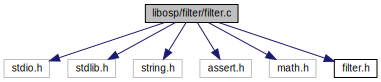
\includegraphics[width=350pt]{filter_8c__incl}
\end{center}
\end{figure}
\subsection*{Data Structures}
\begin{DoxyCompactItemize}
\item 
struct \mbox{\hyperlink{structfilter__t}{filter\+\_\+t}}
\begin{DoxyCompactList}\small\item\em Structure containing filter information. \end{DoxyCompactList}\end{DoxyCompactItemize}
\subsection*{Functions}
\begin{DoxyCompactItemize}
\item 
\mbox{\hyperlink{filter_8h_a69e34b8aa259d2ca0b81b5c95f395bdf}{Filter}} \mbox{\hyperlink{filter_8c_af60877ab9deea7636e6618b2e63ec84f}{filter\+\_\+init}} (const float $\ast$taps, int tap\+\_\+length)
\begin{DoxyCompactList}\small\item\em Initializes filer data structure. \end{DoxyCompactList}\item 
int \mbox{\hyperlink{filter_8c_af0509440b286595b487f0f4eb97670cb}{filter\+\_\+update\+\_\+taps}} (\mbox{\hyperlink{filter_8h_a69e34b8aa259d2ca0b81b5c95f395bdf}{Filter}} obj, float $\ast$taps, int tap\+\_\+length)
\begin{DoxyCompactList}\small\item\em Updates the taps in the Filter data structure N\+O\+TE\+: If the tap length is not the same as what was passed into filter\+\_\+init the function will return an error. We don\textquotesingle{}t change tap length at runtime just what\textquotesingle{}s loaded into the taps. \end{DoxyCompactList}\item 
int \mbox{\hyperlink{filter_8c_ac26376b60c9cd619476f86177abcbd84}{filter\+\_\+get\+\_\+taps}} (\mbox{\hyperlink{filter_8h_a69e34b8aa259d2ca0b81b5c95f395bdf}{Filter}} obj, float $\ast$taps)
\begin{DoxyCompactList}\small\item\em Returns the taps loaded into the taps element in the Filter data structure. \end{DoxyCompactList}\item 
int \mbox{\hyperlink{filter_8c_a1617a39021eb367cd89a15fbd041d83d}{filter\+\_\+get\+\_\+internal\+\_\+buffer}} (\mbox{\hyperlink{filter_8h_a69e34b8aa259d2ca0b81b5c95f395bdf}{Filter}} obj, float $\ast$buf)
\begin{DoxyCompactList}\small\item\em Returns the internal circular buffer. \end{DoxyCompactList}\item 
int \mbox{\hyperlink{filter_8c_a21892025b31d4a556a331b742ecd37d9}{filter\+\_\+get\+\_\+delay}} (\mbox{\hyperlink{filter_8h_a69e34b8aa259d2ca0b81b5c95f395bdf}{Filter}} obj)
\begin{DoxyCompactList}\small\item\em returns the delay of the current filter \end{DoxyCompactList}\item 
void \mbox{\hyperlink{filter_8c_a299844d7458e68c5548821f1adadc673}{D\+S\+P\+F\+\_\+sp\+\_\+fircirc}} (float x\mbox{[}$\,$\mbox{]}, float h\mbox{[}$\,$\mbox{]}, float r\mbox{[}$\,$\mbox{]}, int index, int csize, int nh, size\+\_\+t nr)
\item 
void \mbox{\hyperlink{filter_8c_ac2aadc60ec73a10df6ec442186117a85}{filter\+\_\+proc}} (\mbox{\hyperlink{filter_8h_a69e34b8aa259d2ca0b81b5c95f395bdf}{Filter}} obj, float $\ast$in, float $\ast$out, size\+\_\+t len)
\begin{DoxyCompactList}\small\item\em Filters input signal with current filter, and returns output signal. \end{DoxyCompactList}\item 
void \mbox{\hyperlink{filter_8c_a73f846329181b350960205937c9eb499}{filter\+\_\+flush}} (\mbox{\hyperlink{filter_8h_a69e34b8aa259d2ca0b81b5c95f395bdf}{Filter}} obj, float $\ast$out)
\begin{DoxyCompactList}\small\item\em Flushes the internal buffer of the filter. When the last frame has been processed, there will still exist some residual data on the internal circular buffer. This data would have been used for the next frame\textquotesingle{}s processing, but since we\textquotesingle{}ve reached the last frame, it just sits in memory. In the case of a file-\/based, non-\/realtime test where every sample of the output signal is needed, this can be called after the final frame worth of data. It will return $<$filter\textquotesingle{}s\+\_\+group\+\_\+delay$>$ worth of samples that have been processed with the filter. \end{DoxyCompactList}\item 
int \mbox{\hyperlink{filter_8c_ae0a5a8084cee81b1e417293d2d53f6ed}{filter\+\_\+destroy}} (\mbox{\hyperlink{filter_8h_a69e34b8aa259d2ca0b81b5c95f395bdf}{Filter}} obj)
\begin{DoxyCompactList}\small\item\em Frees and destroys the filter data structure. \end{DoxyCompactList}\end{DoxyCompactItemize}


\subsection{Function Documentation}
\mbox{\Hypertarget{filter_8c_a299844d7458e68c5548821f1adadc673}\label{filter_8c_a299844d7458e68c5548821f1adadc673}} 
\index{filter.\+c@{filter.\+c}!D\+S\+P\+F\+\_\+sp\+\_\+fircirc@{D\+S\+P\+F\+\_\+sp\+\_\+fircirc}}
\index{D\+S\+P\+F\+\_\+sp\+\_\+fircirc@{D\+S\+P\+F\+\_\+sp\+\_\+fircirc}!filter.\+c@{filter.\+c}}
\subsubsection{\texorpdfstring{D\+S\+P\+F\+\_\+sp\+\_\+fircirc()}{DSPF\_sp\_fircirc()}}
{\footnotesize\ttfamily void D\+S\+P\+F\+\_\+sp\+\_\+fircirc (\begin{DoxyParamCaption}\item[{float}]{x\mbox{[}$\,$\mbox{]},  }\item[{float}]{h\mbox{[}$\,$\mbox{]},  }\item[{float}]{r\mbox{[}$\,$\mbox{]},  }\item[{int}]{index,  }\item[{int}]{csize,  }\item[{int}]{nh,  }\item[{size\+\_\+t}]{nr }\end{DoxyParamCaption})}

\mbox{\Hypertarget{filter_8c_ae0a5a8084cee81b1e417293d2d53f6ed}\label{filter_8c_ae0a5a8084cee81b1e417293d2d53f6ed}} 
\index{filter.\+c@{filter.\+c}!filter\+\_\+destroy@{filter\+\_\+destroy}}
\index{filter\+\_\+destroy@{filter\+\_\+destroy}!filter.\+c@{filter.\+c}}
\subsubsection{\texorpdfstring{filter\+\_\+destroy()}{filter\_destroy()}}
{\footnotesize\ttfamily int filter\+\_\+destroy (\begin{DoxyParamCaption}\item[{\mbox{\hyperlink{filter_8h_a69e34b8aa259d2ca0b81b5c95f395bdf}{Filter}}}]{obj }\end{DoxyParamCaption})}



Frees and destroys the filter data structure. 


\begin{DoxyParams}{Parameters}
{\em obj} & Filter data structure \\
\hline
\end{DoxyParams}
\begin{DoxyReturn}{Returns}
Returns 0 on success, -\/1 otherwise 
\end{DoxyReturn}
\mbox{\Hypertarget{filter_8c_a73f846329181b350960205937c9eb499}\label{filter_8c_a73f846329181b350960205937c9eb499}} 
\index{filter.\+c@{filter.\+c}!filter\+\_\+flush@{filter\+\_\+flush}}
\index{filter\+\_\+flush@{filter\+\_\+flush}!filter.\+c@{filter.\+c}}
\subsubsection{\texorpdfstring{filter\+\_\+flush()}{filter\_flush()}}
{\footnotesize\ttfamily void filter\+\_\+flush (\begin{DoxyParamCaption}\item[{\mbox{\hyperlink{filter_8h_a69e34b8aa259d2ca0b81b5c95f395bdf}{Filter}}}]{obj,  }\item[{float $\ast$}]{out }\end{DoxyParamCaption})}



Flushes the internal buffer of the filter. When the last frame has been processed, there will still exist some residual data on the internal circular buffer. This data would have been used for the next frame\textquotesingle{}s processing, but since we\textquotesingle{}ve reached the last frame, it just sits in memory. In the case of a file-\/based, non-\/realtime test where every sample of the output signal is needed, this can be called after the final frame worth of data. It will return $<$filter\textquotesingle{}s\+\_\+group\+\_\+delay$>$ worth of samples that have been processed with the filter. 


\begin{DoxyParams}{Parameters}
{\em obj} & Filter data structure \\
\hline
{\em out} & Output buffer filled with last processed samples \\
\hline
\end{DoxyParams}
\mbox{\Hypertarget{filter_8c_a21892025b31d4a556a331b742ecd37d9}\label{filter_8c_a21892025b31d4a556a331b742ecd37d9}} 
\index{filter.\+c@{filter.\+c}!filter\+\_\+get\+\_\+delay@{filter\+\_\+get\+\_\+delay}}
\index{filter\+\_\+get\+\_\+delay@{filter\+\_\+get\+\_\+delay}!filter.\+c@{filter.\+c}}
\subsubsection{\texorpdfstring{filter\+\_\+get\+\_\+delay()}{filter\_get\_delay()}}
{\footnotesize\ttfamily int filter\+\_\+get\+\_\+delay (\begin{DoxyParamCaption}\item[{\mbox{\hyperlink{filter_8h_a69e34b8aa259d2ca0b81b5c95f395bdf}{Filter}}}]{obj }\end{DoxyParamCaption})}



returns the delay of the current filter 


\begin{DoxyParams}{Parameters}
{\em obj} & Filter data structure\\
\hline
\end{DoxyParams}
\begin{DoxyReturn}{Returns}
Returns the group delay, in samples, of the current filter 
\end{DoxyReturn}
\mbox{\Hypertarget{filter_8c_a1617a39021eb367cd89a15fbd041d83d}\label{filter_8c_a1617a39021eb367cd89a15fbd041d83d}} 
\index{filter.\+c@{filter.\+c}!filter\+\_\+get\+\_\+internal\+\_\+buffer@{filter\+\_\+get\+\_\+internal\+\_\+buffer}}
\index{filter\+\_\+get\+\_\+internal\+\_\+buffer@{filter\+\_\+get\+\_\+internal\+\_\+buffer}!filter.\+c@{filter.\+c}}
\subsubsection{\texorpdfstring{filter\+\_\+get\+\_\+internal\+\_\+buffer()}{filter\_get\_internal\_buffer()}}
{\footnotesize\ttfamily int filter\+\_\+get\+\_\+internal\+\_\+buffer (\begin{DoxyParamCaption}\item[{\mbox{\hyperlink{filter_8h_a69e34b8aa259d2ca0b81b5c95f395bdf}{Filter}}}]{obj,  }\item[{float $\ast$}]{buf }\end{DoxyParamCaption})}



Returns the internal circular buffer. 


\begin{DoxyParams}{Parameters}
{\em obj} & Filter data structure object \\
\hline
{\em buf} & Buffer that will contain the internal circular buffer\textquotesingle{}s elements\\
\hline
\end{DoxyParams}
\begin{DoxyReturn}{Returns}
returns the current index of the circular buffer 
\end{DoxyReturn}
\mbox{\Hypertarget{filter_8c_ac26376b60c9cd619476f86177abcbd84}\label{filter_8c_ac26376b60c9cd619476f86177abcbd84}} 
\index{filter.\+c@{filter.\+c}!filter\+\_\+get\+\_\+taps@{filter\+\_\+get\+\_\+taps}}
\index{filter\+\_\+get\+\_\+taps@{filter\+\_\+get\+\_\+taps}!filter.\+c@{filter.\+c}}
\subsubsection{\texorpdfstring{filter\+\_\+get\+\_\+taps()}{filter\_get\_taps()}}
{\footnotesize\ttfamily int filter\+\_\+get\+\_\+taps (\begin{DoxyParamCaption}\item[{\mbox{\hyperlink{filter_8h_a69e34b8aa259d2ca0b81b5c95f395bdf}{Filter}}}]{obj,  }\item[{float $\ast$}]{taps }\end{DoxyParamCaption})}



Returns the taps loaded into the taps element in the Filter data structure. 


\begin{DoxyParams}{Parameters}
{\em obj} & Filter data structure \\
\hline
{\em taps} & Will contain the currently loaded filter taps \\
\hline
\end{DoxyParams}
\begin{DoxyReturn}{Returns}
Returns the length of the internal filter 
\end{DoxyReturn}
\mbox{\Hypertarget{filter_8c_af60877ab9deea7636e6618b2e63ec84f}\label{filter_8c_af60877ab9deea7636e6618b2e63ec84f}} 
\index{filter.\+c@{filter.\+c}!filter\+\_\+init@{filter\+\_\+init}}
\index{filter\+\_\+init@{filter\+\_\+init}!filter.\+c@{filter.\+c}}
\subsubsection{\texorpdfstring{filter\+\_\+init()}{filter\_init()}}
{\footnotesize\ttfamily \mbox{\hyperlink{filter_8h_a69e34b8aa259d2ca0b81b5c95f395bdf}{Filter}} filter\+\_\+init (\begin{DoxyParamCaption}\item[{const float $\ast$}]{taps,  }\item[{int}]{tap\+\_\+length }\end{DoxyParamCaption})}



Initializes filer data structure. 


\begin{DoxyParams}{Parameters}
{\em taps} & Pointer to filter taps to load into this filter data structure \\
\hline
{\em tap\+\_\+length} & Number of taps pointed to by taps\\
\hline
\end{DoxyParams}
\begin{DoxyReturn}{Returns}
Returns the allocated filter data structure 
\end{DoxyReturn}
\mbox{\Hypertarget{filter_8c_ac2aadc60ec73a10df6ec442186117a85}\label{filter_8c_ac2aadc60ec73a10df6ec442186117a85}} 
\index{filter.\+c@{filter.\+c}!filter\+\_\+proc@{filter\+\_\+proc}}
\index{filter\+\_\+proc@{filter\+\_\+proc}!filter.\+c@{filter.\+c}}
\subsubsection{\texorpdfstring{filter\+\_\+proc()}{filter\_proc()}}
{\footnotesize\ttfamily void filter\+\_\+proc (\begin{DoxyParamCaption}\item[{\mbox{\hyperlink{filter_8h_a69e34b8aa259d2ca0b81b5c95f395bdf}{Filter}}}]{obj,  }\item[{float $\ast$}]{in,  }\item[{float $\ast$}]{out,  }\item[{size\+\_\+t}]{len }\end{DoxyParamCaption})}



Filters input signal with current filter, and returns output signal. 


\begin{DoxyParams}{Parameters}
{\em obj} & Filter data structure \\
\hline
{\em in} & Input signal \\
\hline
{\em out} & Output signal after filtering \\
\hline
{\em len} & The length of the input and output signals (in our implementation, it\textquotesingle{}s one frame size \\
\hline
\end{DoxyParams}
\mbox{\Hypertarget{filter_8c_af0509440b286595b487f0f4eb97670cb}\label{filter_8c_af0509440b286595b487f0f4eb97670cb}} 
\index{filter.\+c@{filter.\+c}!filter\+\_\+update\+\_\+taps@{filter\+\_\+update\+\_\+taps}}
\index{filter\+\_\+update\+\_\+taps@{filter\+\_\+update\+\_\+taps}!filter.\+c@{filter.\+c}}
\subsubsection{\texorpdfstring{filter\+\_\+update\+\_\+taps()}{filter\_update\_taps()}}
{\footnotesize\ttfamily int filter\+\_\+update\+\_\+taps (\begin{DoxyParamCaption}\item[{\mbox{\hyperlink{filter_8h_a69e34b8aa259d2ca0b81b5c95f395bdf}{Filter}}}]{obj,  }\item[{float $\ast$}]{taps,  }\item[{int}]{tap\+\_\+length }\end{DoxyParamCaption})}



Updates the taps in the Filter data structure N\+O\+TE\+: If the tap length is not the same as what was passed into filter\+\_\+init the function will return an error. We don\textquotesingle{}t change tap length at runtime just what\textquotesingle{}s loaded into the taps. 


\begin{DoxyParams}{Parameters}
{\em obj} & Filter data structure \\
\hline
{\em taps} & New taps to load into old taps\textquotesingle{} place \\
\hline
{\em tap\+\_\+length} & Number of taps to load into the taps\\
\hline
\end{DoxyParams}
\begin{DoxyReturn}{Returns}
Returns 0 on success, -\/1 if the tap\+\_\+length parameter does not match the tap length that was set up in filter\+\_\+init 
\end{DoxyReturn}
\begin{DoxySeeAlso}{See also}
\mbox{\hyperlink{filter_8h_af60877ab9deea7636e6618b2e63ec84f}{filter\+\_\+init}} 
\end{DoxySeeAlso}

\input{filter_8h}
\hypertarget{coeffs_8h}{}\section{libosp/osp\+\_\+process/coeffs.h File Reference}
\label{coeffs_8h}\index{libosp/osp\+\_\+process/coeffs.\+h@{libosp/osp\+\_\+process/coeffs.\+h}}
{\ttfamily \#include \char`\"{}constants.\+h\char`\"{}}\newline
Include dependency graph for coeffs.\+h\+:\nopagebreak
\begin{figure}[H]
\begin{center}
\leavevmode
\includegraphics[width=182pt]{coeffs_8h__incl}
\end{center}
\end{figure}
This graph shows which files directly or indirectly include this file\+:\nopagebreak
\begin{figure}[H]
\begin{center}
\leavevmode
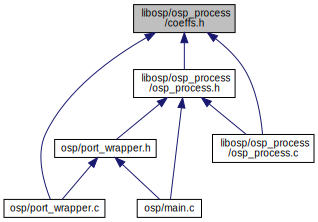
\includegraphics[width=350pt]{coeffs_8h__dep__incl}
\end{center}
\end{figure}
\subsection*{Macros}
\begin{DoxyCompactItemize}
\item 
\#define \mbox{\hyperlink{coeffs_8h_a6242a25f9d996f0cc4f4cdb911218b75}{A\+R\+R\+A\+Y\+\_\+\+S\+I\+ZE}}(x)~(sizeof((x)) / sizeof((x)\mbox{[}0\mbox{]}))
\item 
\#define \mbox{\hyperlink{coeffs_8h_ad32ac4875a4561a20175c2d6a57cee49}{H\+P\+F\+\_\+\+T\+A\+PS}}~4
\begin{DoxyCompactList}\small\item\em Pre-\/whitening filter tap length. \end{DoxyCompactList}\item 
\#define \mbox{\hyperlink{coeffs_8h_a8ab9ea24d07761ec9ccfa381bffac6eb}{B\+L\+F\+\_\+\+T\+A\+PS}}~4
\begin{DoxyCompactList}\small\item\em Band-\/limited filter tap length. \end{DoxyCompactList}\end{DoxyCompactItemize}
\subsection*{Variables}
\begin{DoxyCompactItemize}
\item 
static const float \mbox{\hyperlink{coeffs_8h_a628bfda8ff99b4ecdd3ebb99c2da7f1c}{hpf\+\_\+taps}} \mbox{[}\mbox{\hyperlink{coeffs_8h_ad32ac4875a4561a20175c2d6a57cee49}{H\+P\+F\+\_\+\+T\+A\+PS}}\mbox{]}
\begin{DoxyCompactList}\small\item\em Pre-\/whitening filter taps. \end{DoxyCompactList}\item 
static const float \mbox{\hyperlink{coeffs_8h_ae7296be7fe6800f75d74a13df257f839}{blf\+\_\+taps}} \mbox{[}\mbox{\hyperlink{coeffs_8h_a8ab9ea24d07761ec9ccfa381bffac6eb}{B\+L\+F\+\_\+\+T\+A\+PS}}\mbox{]}
\begin{DoxyCompactList}\small\item\em Band-\/limited filter taps. \end{DoxyCompactList}\end{DoxyCompactItemize}


\subsection{Macro Definition Documentation}
\mbox{\Hypertarget{coeffs_8h_a6242a25f9d996f0cc4f4cdb911218b75}\label{coeffs_8h_a6242a25f9d996f0cc4f4cdb911218b75}} 
\index{coeffs.\+h@{coeffs.\+h}!A\+R\+R\+A\+Y\+\_\+\+S\+I\+ZE@{A\+R\+R\+A\+Y\+\_\+\+S\+I\+ZE}}
\index{A\+R\+R\+A\+Y\+\_\+\+S\+I\+ZE@{A\+R\+R\+A\+Y\+\_\+\+S\+I\+ZE}!coeffs.\+h@{coeffs.\+h}}
\subsubsection{\texorpdfstring{A\+R\+R\+A\+Y\+\_\+\+S\+I\+ZE}{ARRAY\_SIZE}}
{\footnotesize\ttfamily \#define A\+R\+R\+A\+Y\+\_\+\+S\+I\+ZE(\begin{DoxyParamCaption}\item[{}]{x }\end{DoxyParamCaption})~(sizeof((x)) / sizeof((x)\mbox{[}0\mbox{]}))}

\mbox{\Hypertarget{coeffs_8h_a8ab9ea24d07761ec9ccfa381bffac6eb}\label{coeffs_8h_a8ab9ea24d07761ec9ccfa381bffac6eb}} 
\index{coeffs.\+h@{coeffs.\+h}!B\+L\+F\+\_\+\+T\+A\+PS@{B\+L\+F\+\_\+\+T\+A\+PS}}
\index{B\+L\+F\+\_\+\+T\+A\+PS@{B\+L\+F\+\_\+\+T\+A\+PS}!coeffs.\+h@{coeffs.\+h}}
\subsubsection{\texorpdfstring{B\+L\+F\+\_\+\+T\+A\+PS}{BLF\_TAPS}}
{\footnotesize\ttfamily \#define B\+L\+F\+\_\+\+T\+A\+PS~4}



Band-\/limited filter tap length. 

\mbox{\Hypertarget{coeffs_8h_ad32ac4875a4561a20175c2d6a57cee49}\label{coeffs_8h_ad32ac4875a4561a20175c2d6a57cee49}} 
\index{coeffs.\+h@{coeffs.\+h}!H\+P\+F\+\_\+\+T\+A\+PS@{H\+P\+F\+\_\+\+T\+A\+PS}}
\index{H\+P\+F\+\_\+\+T\+A\+PS@{H\+P\+F\+\_\+\+T\+A\+PS}!coeffs.\+h@{coeffs.\+h}}
\subsubsection{\texorpdfstring{H\+P\+F\+\_\+\+T\+A\+PS}{HPF\_TAPS}}
{\footnotesize\ttfamily \#define H\+P\+F\+\_\+\+T\+A\+PS~4}



Pre-\/whitening filter tap length. 



\subsection{Variable Documentation}
\mbox{\Hypertarget{coeffs_8h_ae7296be7fe6800f75d74a13df257f839}\label{coeffs_8h_ae7296be7fe6800f75d74a13df257f839}} 
\index{coeffs.\+h@{coeffs.\+h}!blf\+\_\+taps@{blf\+\_\+taps}}
\index{blf\+\_\+taps@{blf\+\_\+taps}!coeffs.\+h@{coeffs.\+h}}
\subsubsection{\texorpdfstring{blf\+\_\+taps}{blf\_taps}}
{\footnotesize\ttfamily const float blf\+\_\+taps\mbox{[}\mbox{\hyperlink{coeffs_8h_a8ab9ea24d07761ec9ccfa381bffac6eb}{B\+L\+F\+\_\+\+T\+A\+PS}}\mbox{]}\hspace{0.3cm}{\ttfamily [static]}}

{\bfseries Initial value\+:}
\begin{DoxyCode}
= \{
    -0.0876,
    -0.7904,
    0.7904,
    0.0876
\}
\end{DoxyCode}


Band-\/limited filter taps. 

\mbox{\Hypertarget{coeffs_8h_a628bfda8ff99b4ecdd3ebb99c2da7f1c}\label{coeffs_8h_a628bfda8ff99b4ecdd3ebb99c2da7f1c}} 
\index{coeffs.\+h@{coeffs.\+h}!hpf\+\_\+taps@{hpf\+\_\+taps}}
\index{hpf\+\_\+taps@{hpf\+\_\+taps}!coeffs.\+h@{coeffs.\+h}}
\subsubsection{\texorpdfstring{hpf\+\_\+taps}{hpf\_taps}}
{\footnotesize\ttfamily const float hpf\+\_\+taps\mbox{[}\mbox{\hyperlink{coeffs_8h_ad32ac4875a4561a20175c2d6a57cee49}{H\+P\+F\+\_\+\+T\+A\+PS}}\mbox{]}\hspace{0.3cm}{\ttfamily [static]}}

{\bfseries Initial value\+:}
\begin{DoxyCode}
= \{
    0.1170,
    -0.6034,
    0.6034,
    -0.1170
\}
\end{DoxyCode}


Pre-\/whitening filter taps. 


\hypertarget{osp__process_8c}{}\section{libosp/osp\+\_\+process/osp\+\_\+process.c File Reference}
\label{osp__process_8c}\index{libosp/osp\+\_\+process/osp\+\_\+process.\+c@{libosp/osp\+\_\+process/osp\+\_\+process.\+c}}
{\ttfamily \#include $<$stdio.\+h$>$}\newline
{\ttfamily \#include $<$stdlib.\+h$>$}\newline
{\ttfamily \#include $<$string.\+h$>$}\newline
{\ttfamily \#include \char`\"{}constants.\+h\char`\"{}}\newline
{\ttfamily \#include \char`\"{}logger.\+h\char`\"{}}\newline
{\ttfamily \#include \char`\"{}speech\+\_\+enhancement.\+h\char`\"{}}\newline
{\ttfamily \#include \char`\"{}osp\+\_\+process.\+h\char`\"{}}\newline
{\ttfamily \#include \char`\"{}utilities.\+h\char`\"{}}\newline
{\ttfamily \#include \char`\"{}filter.\+h\char`\"{}}\newline
{\ttfamily \#include \char`\"{}coeffs.\+h\char`\"{}}\newline
{\ttfamily \#include \char`\"{}afc.\+h\char`\"{}}\newline
{\ttfamily \#include \char`\"{}delay\+\_\+line.\+h\char`\"{}}\newline
{\ttfamily \#include \char`\"{}array\+\_\+utilities.\+h\char`\"{}}\newline
{\ttfamily \#include \char`\"{}peak\+\_\+detect.\+h\char`\"{}}\newline
{\ttfamily \#include \char`\"{}wdrc.\+h\char`\"{}}\newline
{\ttfamily \#include \char`\"{}wdrc\+\_\+mpo\+\_\+support.\+h\char`\"{}}\newline
{\ttfamily \#include \char`\"{}mpo.\+h\char`\"{}}\newline
Include dependency graph for osp\+\_\+process.\+c\+:\nopagebreak
\begin{figure}[H]
\begin{center}
\leavevmode
\includegraphics[width=350pt]{osp__process_8c__incl}
\end{center}
\end{figure}
\subsection*{Macros}
\begin{DoxyCompactItemize}
\item 
\#define \mbox{\hyperlink{osp__process_8c_a35028ea7fc0cef3cdc0ce4fbd2ff25a4}{F\+E\+E\+D\+B\+A\+C\+K\+\_\+\+E\+S\+T\+\_\+\+D\+E\+L\+AY}}~100
\begin{DoxyCompactList}\small\item\em Feedback delay in samples. For file loopback its 0. For real-\/time processing one needs to account for I/O delay. \end{DoxyCompactList}\item 
\#define \mbox{\hyperlink{osp__process_8c_a5f1590d4ac46cd4c58167f767d284ef7}{S\+T\+E\+R\+EO}}
\begin{DoxyCompactList}\small\item\em Toggle for stereo and mono. \end{DoxyCompactList}\end{DoxyCompactItemize}
\subsection*{Functions}
\begin{DoxyCompactItemize}
\item 
static void \mbox{\hyperlink{osp__process_8c_a5e03afe3816964e6052931a58b754d99}{osp\+\_\+process\+\_\+ha}} (\mbox{\hyperlink{constants_8h_a2d1d78531fe12807c3852488556d5a4b}{osp\+\_\+user\+\_\+data}} $\ast$osp, \mbox{\hyperlink{filter_8h_a69e34b8aa259d2ca0b81b5c95f395bdf}{Filter}} $\ast$filter, \mbox{\hyperlink{peak__detect_8h_a152d14cd03f6e1ac947c95921da5507c}{Peak\+\_\+detect}} pd, float $\ast$e\+\_\+n, float $\ast$s\+\_\+n, size\+\_\+t len)
\begin{DoxyCompactList}\small\item\em Function that performs basic Hearing Aid (HA) processing on a single channel. \end{DoxyCompactList}\item 
int \mbox{\hyperlink{osp__process_8c_aabb5c0280f6d5cd0cce725a00533978f}{osp\+\_\+init}} (unsigned int frame\+\_\+size, int sample\+\_\+rate, \mbox{\hyperlink{constants_8h_a2d1d78531fe12807c3852488556d5a4b}{osp\+\_\+user\+\_\+data}} $\ast$osp\+\_\+data)
\begin{DoxyCompactList}\small\item\em This file groups all of the different O\+SP library calls in one place. This is more of an example way of using the different parts of the O\+SP libraries to implement a hearing aid algorith with M\+HA and A\+FC all in one place. \end{DoxyCompactList}\item 
void \mbox{\hyperlink{osp__process_8c_a6c8f16a08d0ce2a2b4989861253a51f5}{osp\+\_\+process\+\_\+audio}} (\mbox{\hyperlink{constants_8h_a2d1d78531fe12807c3852488556d5a4b}{osp\+\_\+user\+\_\+data}} $\ast$osp, float $\ast$x\+\_\+nL, float $\ast$x\+\_\+nR, float $\ast$outL, float $\ast$outR, size\+\_\+t len)
\begin{DoxyCompactList}\small\item\em Function to perform Master Hearing Aid (M\+HA) processing on the input signal for both channels. \end{DoxyCompactList}\item 
unsigned int \mbox{\hyperlink{osp__process_8c_afa87b8384a65fb6f6a12ac92297c9961}{osp\+\_\+get\+\_\+num\+\_\+bands}} ()
\begin{DoxyCompactList}\small\item\em Function to get the number of Sub-\/\+Bands. \end{DoxyCompactList}\item 
void \mbox{\hyperlink{osp__process_8c_af0a98853e0b3bce6a93cb88c1839723f}{osp\+\_\+close}} ()
\begin{DoxyCompactList}\small\item\em Wrapper function to free all the modules of Master Hearing Aid (M\+HA) \end{DoxyCompactList}\item 
void \mbox{\hyperlink{osp__process_8c_a37765f5c4d9ab3f3569947503b97a6c6}{osp\+\_\+dump\+\_\+afc\+\_\+filter}} ()
\begin{DoxyCompactList}\small\item\em Function to dump A\+FC filter taps for both left and right channels. \end{DoxyCompactList}\item 
void \mbox{\hyperlink{osp__process_8c_a12fc7be1c06d51523df05f460e91d097}{osp\+\_\+data\+\_\+init}} (\mbox{\hyperlink{constants_8h_a2d1d78531fe12807c3852488556d5a4b}{osp\+\_\+user\+\_\+data}} $\ast$user\+\_\+data)
\begin{DoxyCompactList}\small\item\em Helper function for initializing Master Hearing Aid (M\+HA) parameters. \end{DoxyCompactList}\item 
void \mbox{\hyperlink{osp__process_8c_a1b9e53a67adfda315e3fe93862361d22}{osp\+\_\+data\+\_\+set\+\_\+gain}} (\mbox{\hyperlink{constants_8h_a2d1d78531fe12807c3852488556d5a4b}{osp\+\_\+user\+\_\+data}} $\ast$user\+\_\+data, int gain)
\begin{DoxyCompactList}\small\item\em Helper function for initializing gain parameters for W\+D\+RC with a constant gain. \end{DoxyCompactList}\item 
void \mbox{\hyperlink{osp__process_8c_a6f9f5ada6b7f84af9827bbb1cbe68d3d}{osp\+\_\+data\+\_\+set\+\_\+nh}} (\mbox{\hyperlink{constants_8h_a2d1d78531fe12807c3852488556d5a4b}{osp\+\_\+user\+\_\+data}} $\ast$user\+\_\+data)
\begin{DoxyCompactList}\small\item\em Helper function for initializing gain parameters for W\+D\+RC with NH audiogram. \end{DoxyCompactList}\item 
void \mbox{\hyperlink{osp__process_8c_aa23c1072681c057f945a6d22d7659934}{osp\+\_\+data\+\_\+set\+\_\+n2}} (\mbox{\hyperlink{constants_8h_a2d1d78531fe12807c3852488556d5a4b}{osp\+\_\+user\+\_\+data}} $\ast$user\+\_\+data)
\begin{DoxyCompactList}\small\item\em Helper function for initializing gain parameters for W\+D\+RC with N2 audiogram. \end{DoxyCompactList}\item 
void \mbox{\hyperlink{osp__process_8c_ae7da3f44c97ca3e1ec342f2410015845}{osp\+\_\+data\+\_\+set\+\_\+n4}} (\mbox{\hyperlink{constants_8h_a2d1d78531fe12807c3852488556d5a4b}{osp\+\_\+user\+\_\+data}} $\ast$user\+\_\+data)
\begin{DoxyCompactList}\small\item\em Helper function for initializing gain parameters for W\+D\+RC with N4 audiogram. \end{DoxyCompactList}\item 
void \mbox{\hyperlink{osp__process_8c_aeb2474bd6b995d8ad289bfb1ce9b91c9}{osp\+\_\+data\+\_\+set\+\_\+s2}} (\mbox{\hyperlink{constants_8h_a2d1d78531fe12807c3852488556d5a4b}{osp\+\_\+user\+\_\+data}} $\ast$user\+\_\+data)
\begin{DoxyCompactList}\small\item\em Helper function for initializing gain parameters for W\+D\+RC with S2 audiogram. \end{DoxyCompactList}\end{DoxyCompactItemize}
\subsection*{Variables}
\begin{DoxyCompactItemize}
\item 
static \mbox{\hyperlink{filter_8h_a69e34b8aa259d2ca0b81b5c95f395bdf}{Filter}} \mbox{\hyperlink{osp__process_8c_a7c99ae65957762007fcd93018842ed12}{filterL}} \mbox{[}\mbox{\hyperlink{constants_8h_a19441d7b9be72492ed93a440085e53be}{N\+U\+M\+\_\+\+B\+A\+N\+DS}}\mbox{]}
\item 
static \mbox{\hyperlink{filter_8h_a69e34b8aa259d2ca0b81b5c95f395bdf}{Filter}} \mbox{\hyperlink{osp__process_8c_a1768daa4a1e3e9e2e2d5327315ba69f9}{filterR}} \mbox{[}\mbox{\hyperlink{constants_8h_a19441d7b9be72492ed93a440085e53be}{N\+U\+M\+\_\+\+B\+A\+N\+DS}}\mbox{]}
\item 
static \mbox{\hyperlink{filter_8h_a69e34b8aa259d2ca0b81b5c95f395bdf}{Filter}} \mbox{\hyperlink{osp__process_8c_a0d1d77ea7cad8796f93e5185af5d04b6}{synthetic\+\_\+feedback\+\_\+filter\+\_\+left}}
\item 
static \mbox{\hyperlink{filter_8h_a69e34b8aa259d2ca0b81b5c95f395bdf}{Filter}} \mbox{\hyperlink{osp__process_8c_a245b5b6521a6c8aa806c31919532ee0b}{synthetic\+\_\+feedback\+\_\+filter\+\_\+right}}
\item 
static \mbox{\hyperlink{peak__detect_8h_a152d14cd03f6e1ac947c95921da5507c}{Peak\+\_\+detect}} \mbox{\hyperlink{osp__process_8c_a3c18e558d4aff166f6be1cd1fa271ff1}{pdL}}
\item 
static \mbox{\hyperlink{peak__detect_8h_a152d14cd03f6e1ac947c95921da5507c}{Peak\+\_\+detect}} \mbox{\hyperlink{osp__process_8c_aa630bd455bf668501cc2c91822cb4d2b}{pdR}}
\item 
static \mbox{\hyperlink{afc_8h_a18f5ff6b916f548f1d14d1e48ec23908}{Afc}} \mbox{\hyperlink{osp__process_8c_a1b0e0576d2848078cb3c36c87014bff5}{afc\+\_\+left}}
\item 
static \mbox{\hyperlink{afc_8h_a18f5ff6b916f548f1d14d1e48ec23908}{Afc}} \mbox{\hyperlink{osp__process_8c_a79945a59c824205d3853b2488639dcda}{afc\+\_\+right}}
\item 
static \mbox{\hyperlink{delay__line_8h_aa62b49f8bfee0c3a174896c9b446d68d}{Delay\+\_\+\+Line}} \mbox{\hyperlink{osp__process_8c_adfcf80bfcebee0007f158d88b724f531}{delay\+\_\+line\+\_\+left}}
\item 
static \mbox{\hyperlink{delay__line_8h_aa62b49f8bfee0c3a174896c9b446d68d}{Delay\+\_\+\+Line}} \mbox{\hyperlink{osp__process_8c_af011450742dbabbc02c0fb1a3903a884}{delay\+\_\+line\+\_\+right}}
\end{DoxyCompactItemize}


\subsection{Macro Definition Documentation}
\mbox{\Hypertarget{osp__process_8c_a35028ea7fc0cef3cdc0ce4fbd2ff25a4}\label{osp__process_8c_a35028ea7fc0cef3cdc0ce4fbd2ff25a4}} 
\index{osp\+\_\+process.\+c@{osp\+\_\+process.\+c}!F\+E\+E\+D\+B\+A\+C\+K\+\_\+\+E\+S\+T\+\_\+\+D\+E\+L\+AY@{F\+E\+E\+D\+B\+A\+C\+K\+\_\+\+E\+S\+T\+\_\+\+D\+E\+L\+AY}}
\index{F\+E\+E\+D\+B\+A\+C\+K\+\_\+\+E\+S\+T\+\_\+\+D\+E\+L\+AY@{F\+E\+E\+D\+B\+A\+C\+K\+\_\+\+E\+S\+T\+\_\+\+D\+E\+L\+AY}!osp\+\_\+process.\+c@{osp\+\_\+process.\+c}}
\subsubsection{\texorpdfstring{F\+E\+E\+D\+B\+A\+C\+K\+\_\+\+E\+S\+T\+\_\+\+D\+E\+L\+AY}{FEEDBACK\_EST\_DELAY}}
{\footnotesize\ttfamily \#define F\+E\+E\+D\+B\+A\+C\+K\+\_\+\+E\+S\+T\+\_\+\+D\+E\+L\+AY~100}



Feedback delay in samples. For file loopback its 0. For real-\/time processing one needs to account for I/O delay. 

\mbox{\Hypertarget{osp__process_8c_a5f1590d4ac46cd4c58167f767d284ef7}\label{osp__process_8c_a5f1590d4ac46cd4c58167f767d284ef7}} 
\index{osp\+\_\+process.\+c@{osp\+\_\+process.\+c}!S\+T\+E\+R\+EO@{S\+T\+E\+R\+EO}}
\index{S\+T\+E\+R\+EO@{S\+T\+E\+R\+EO}!osp\+\_\+process.\+c@{osp\+\_\+process.\+c}}
\subsubsection{\texorpdfstring{S\+T\+E\+R\+EO}{STEREO}}
{\footnotesize\ttfamily \#define S\+T\+E\+R\+EO}



Toggle for stereo and mono. 



\subsection{Function Documentation}
\mbox{\Hypertarget{osp__process_8c_af0a98853e0b3bce6a93cb88c1839723f}\label{osp__process_8c_af0a98853e0b3bce6a93cb88c1839723f}} 
\index{osp\+\_\+process.\+c@{osp\+\_\+process.\+c}!osp\+\_\+close@{osp\+\_\+close}}
\index{osp\+\_\+close@{osp\+\_\+close}!osp\+\_\+process.\+c@{osp\+\_\+process.\+c}}
\subsubsection{\texorpdfstring{osp\+\_\+close()}{osp\_close()}}
{\footnotesize\ttfamily void osp\+\_\+close (\begin{DoxyParamCaption}{ }\end{DoxyParamCaption})}



Wrapper function to free all the modules of Master Hearing Aid (M\+HA) 

\mbox{\Hypertarget{osp__process_8c_a12fc7be1c06d51523df05f460e91d097}\label{osp__process_8c_a12fc7be1c06d51523df05f460e91d097}} 
\index{osp\+\_\+process.\+c@{osp\+\_\+process.\+c}!osp\+\_\+data\+\_\+init@{osp\+\_\+data\+\_\+init}}
\index{osp\+\_\+data\+\_\+init@{osp\+\_\+data\+\_\+init}!osp\+\_\+process.\+c@{osp\+\_\+process.\+c}}
\subsubsection{\texorpdfstring{osp\+\_\+data\+\_\+init()}{osp\_data\_init()}}
{\footnotesize\ttfamily void osp\+\_\+data\+\_\+init (\begin{DoxyParamCaption}\item[{\mbox{\hyperlink{constants_8h_a2d1d78531fe12807c3852488556d5a4b}{osp\+\_\+user\+\_\+data}} $\ast$}]{user\+\_\+data }\end{DoxyParamCaption})}



Helper function for initializing Master Hearing Aid (M\+HA) parameters. 

\begin{DoxySeeAlso}{See also}
\mbox{\hyperlink{constants_8h_a2d1d78531fe12807c3852488556d5a4b}{osp\+\_\+user\+\_\+data}} 

\mbox{\hyperlink{osp__process_8h_a1b9e53a67adfda315e3fe93862361d22}{osp\+\_\+data\+\_\+set\+\_\+gain}}, \mbox{\hyperlink{osp__process_8h_a6f9f5ada6b7f84af9827bbb1cbe68d3d}{osp\+\_\+data\+\_\+set\+\_\+nh}}, \mbox{\hyperlink{osp__process_8h_aa23c1072681c057f945a6d22d7659934}{osp\+\_\+data\+\_\+set\+\_\+n2}} ,\mbox{\hyperlink{osp__process_8h_ae7da3f44c97ca3e1ec342f2410015845}{osp\+\_\+data\+\_\+set\+\_\+n4}} ,\mbox{\hyperlink{osp__process_8h_aeb2474bd6b995d8ad289bfb1ce9b91c9}{osp\+\_\+data\+\_\+set\+\_\+s2}} 
\end{DoxySeeAlso}

\begin{DoxyParams}{Parameters}
{\em user\+\_\+data} & Pointer to an osp\+\_\+user\+\_\+data instance which will be allocated in the function \\
\hline
\end{DoxyParams}
\mbox{\Hypertarget{osp__process_8c_a1b9e53a67adfda315e3fe93862361d22}\label{osp__process_8c_a1b9e53a67adfda315e3fe93862361d22}} 
\index{osp\+\_\+process.\+c@{osp\+\_\+process.\+c}!osp\+\_\+data\+\_\+set\+\_\+gain@{osp\+\_\+data\+\_\+set\+\_\+gain}}
\index{osp\+\_\+data\+\_\+set\+\_\+gain@{osp\+\_\+data\+\_\+set\+\_\+gain}!osp\+\_\+process.\+c@{osp\+\_\+process.\+c}}
\subsubsection{\texorpdfstring{osp\+\_\+data\+\_\+set\+\_\+gain()}{osp\_data\_set\_gain()}}
{\footnotesize\ttfamily void osp\+\_\+data\+\_\+set\+\_\+gain (\begin{DoxyParamCaption}\item[{\mbox{\hyperlink{constants_8h_a2d1d78531fe12807c3852488556d5a4b}{osp\+\_\+user\+\_\+data}} $\ast$}]{user\+\_\+data,  }\item[{int}]{gain }\end{DoxyParamCaption})}



Helper function for initializing gain parameters for W\+D\+RC with a constant gain. 

\begin{DoxySeeAlso}{See also}
\mbox{\hyperlink{constants_8h_a2d1d78531fe12807c3852488556d5a4b}{osp\+\_\+user\+\_\+data}} 

\mbox{\hyperlink{osp__process_8h_a1b9e53a67adfda315e3fe93862361d22}{osp\+\_\+data\+\_\+set\+\_\+gain}}, \mbox{\hyperlink{osp__process_8h_a6f9f5ada6b7f84af9827bbb1cbe68d3d}{osp\+\_\+data\+\_\+set\+\_\+nh}}, \mbox{\hyperlink{osp__process_8h_aa23c1072681c057f945a6d22d7659934}{osp\+\_\+data\+\_\+set\+\_\+n2}} ,\mbox{\hyperlink{osp__process_8h_ae7da3f44c97ca3e1ec342f2410015845}{osp\+\_\+data\+\_\+set\+\_\+n4}} ,\mbox{\hyperlink{osp__process_8h_aeb2474bd6b995d8ad289bfb1ce9b91c9}{osp\+\_\+data\+\_\+set\+\_\+s2}} 
\end{DoxySeeAlso}

\begin{DoxyParams}{Parameters}
{\em user\+\_\+data} & Pointer to the instance of osp\+\_\+user\+\_\+data initialized by osp\+\_\+data\+\_\+init \\
\hline
{\em gain} & The constant gain value \\
\hline
\end{DoxyParams}
\mbox{\Hypertarget{osp__process_8c_aa23c1072681c057f945a6d22d7659934}\label{osp__process_8c_aa23c1072681c057f945a6d22d7659934}} 
\index{osp\+\_\+process.\+c@{osp\+\_\+process.\+c}!osp\+\_\+data\+\_\+set\+\_\+n2@{osp\+\_\+data\+\_\+set\+\_\+n2}}
\index{osp\+\_\+data\+\_\+set\+\_\+n2@{osp\+\_\+data\+\_\+set\+\_\+n2}!osp\+\_\+process.\+c@{osp\+\_\+process.\+c}}
\subsubsection{\texorpdfstring{osp\+\_\+data\+\_\+set\+\_\+n2()}{osp\_data\_set\_n2()}}
{\footnotesize\ttfamily void osp\+\_\+data\+\_\+set\+\_\+n2 (\begin{DoxyParamCaption}\item[{\mbox{\hyperlink{constants_8h_a2d1d78531fe12807c3852488556d5a4b}{osp\+\_\+user\+\_\+data}} $\ast$}]{user\+\_\+data }\end{DoxyParamCaption})}



Helper function for initializing gain parameters for W\+D\+RC with N2 audiogram. 

\begin{DoxySeeAlso}{See also}
\mbox{\hyperlink{constants_8h_a2d1d78531fe12807c3852488556d5a4b}{osp\+\_\+user\+\_\+data}} 

\mbox{\hyperlink{osp__process_8h_a1b9e53a67adfda315e3fe93862361d22}{osp\+\_\+data\+\_\+set\+\_\+gain}}, \mbox{\hyperlink{osp__process_8h_a6f9f5ada6b7f84af9827bbb1cbe68d3d}{osp\+\_\+data\+\_\+set\+\_\+nh}}, \mbox{\hyperlink{osp__process_8h_aa23c1072681c057f945a6d22d7659934}{osp\+\_\+data\+\_\+set\+\_\+n2}} ,\mbox{\hyperlink{osp__process_8h_ae7da3f44c97ca3e1ec342f2410015845}{osp\+\_\+data\+\_\+set\+\_\+n4}} ,\mbox{\hyperlink{osp__process_8h_aeb2474bd6b995d8ad289bfb1ce9b91c9}{osp\+\_\+data\+\_\+set\+\_\+s2}} 
\end{DoxySeeAlso}

\begin{DoxyParams}{Parameters}
{\em user\+\_\+data} & Pointer to the instance of osp\+\_\+user\+\_\+data initialized by osp\+\_\+data\+\_\+init \\
\hline
\end{DoxyParams}
\mbox{\Hypertarget{osp__process_8c_ae7da3f44c97ca3e1ec342f2410015845}\label{osp__process_8c_ae7da3f44c97ca3e1ec342f2410015845}} 
\index{osp\+\_\+process.\+c@{osp\+\_\+process.\+c}!osp\+\_\+data\+\_\+set\+\_\+n4@{osp\+\_\+data\+\_\+set\+\_\+n4}}
\index{osp\+\_\+data\+\_\+set\+\_\+n4@{osp\+\_\+data\+\_\+set\+\_\+n4}!osp\+\_\+process.\+c@{osp\+\_\+process.\+c}}
\subsubsection{\texorpdfstring{osp\+\_\+data\+\_\+set\+\_\+n4()}{osp\_data\_set\_n4()}}
{\footnotesize\ttfamily void osp\+\_\+data\+\_\+set\+\_\+n4 (\begin{DoxyParamCaption}\item[{\mbox{\hyperlink{constants_8h_a2d1d78531fe12807c3852488556d5a4b}{osp\+\_\+user\+\_\+data}} $\ast$}]{user\+\_\+data }\end{DoxyParamCaption})}



Helper function for initializing gain parameters for W\+D\+RC with N4 audiogram. 

\begin{DoxySeeAlso}{See also}
\mbox{\hyperlink{constants_8h_a2d1d78531fe12807c3852488556d5a4b}{osp\+\_\+user\+\_\+data}} 

\mbox{\hyperlink{osp__process_8h_a1b9e53a67adfda315e3fe93862361d22}{osp\+\_\+data\+\_\+set\+\_\+gain}}, \mbox{\hyperlink{osp__process_8h_a6f9f5ada6b7f84af9827bbb1cbe68d3d}{osp\+\_\+data\+\_\+set\+\_\+nh}}, \mbox{\hyperlink{osp__process_8h_aa23c1072681c057f945a6d22d7659934}{osp\+\_\+data\+\_\+set\+\_\+n2}} ,\mbox{\hyperlink{osp__process_8h_ae7da3f44c97ca3e1ec342f2410015845}{osp\+\_\+data\+\_\+set\+\_\+n4}} ,\mbox{\hyperlink{osp__process_8h_aeb2474bd6b995d8ad289bfb1ce9b91c9}{osp\+\_\+data\+\_\+set\+\_\+s2}} 
\end{DoxySeeAlso}

\begin{DoxyParams}{Parameters}
{\em user\+\_\+data} & Pointer to the instance of osp\+\_\+user\+\_\+data initialized by osp\+\_\+data\+\_\+init \\
\hline
\end{DoxyParams}
\mbox{\Hypertarget{osp__process_8c_a6f9f5ada6b7f84af9827bbb1cbe68d3d}\label{osp__process_8c_a6f9f5ada6b7f84af9827bbb1cbe68d3d}} 
\index{osp\+\_\+process.\+c@{osp\+\_\+process.\+c}!osp\+\_\+data\+\_\+set\+\_\+nh@{osp\+\_\+data\+\_\+set\+\_\+nh}}
\index{osp\+\_\+data\+\_\+set\+\_\+nh@{osp\+\_\+data\+\_\+set\+\_\+nh}!osp\+\_\+process.\+c@{osp\+\_\+process.\+c}}
\subsubsection{\texorpdfstring{osp\+\_\+data\+\_\+set\+\_\+nh()}{osp\_data\_set\_nh()}}
{\footnotesize\ttfamily void osp\+\_\+data\+\_\+set\+\_\+nh (\begin{DoxyParamCaption}\item[{\mbox{\hyperlink{constants_8h_a2d1d78531fe12807c3852488556d5a4b}{osp\+\_\+user\+\_\+data}} $\ast$}]{user\+\_\+data }\end{DoxyParamCaption})}



Helper function for initializing gain parameters for W\+D\+RC with NH audiogram. 

\begin{DoxySeeAlso}{See also}
\mbox{\hyperlink{constants_8h_a2d1d78531fe12807c3852488556d5a4b}{osp\+\_\+user\+\_\+data}} 

\mbox{\hyperlink{osp__process_8h_a1b9e53a67adfda315e3fe93862361d22}{osp\+\_\+data\+\_\+set\+\_\+gain}}, \mbox{\hyperlink{osp__process_8h_a6f9f5ada6b7f84af9827bbb1cbe68d3d}{osp\+\_\+data\+\_\+set\+\_\+nh}}, \mbox{\hyperlink{osp__process_8h_aa23c1072681c057f945a6d22d7659934}{osp\+\_\+data\+\_\+set\+\_\+n2}} ,\mbox{\hyperlink{osp__process_8h_ae7da3f44c97ca3e1ec342f2410015845}{osp\+\_\+data\+\_\+set\+\_\+n4}} ,\mbox{\hyperlink{osp__process_8h_aeb2474bd6b995d8ad289bfb1ce9b91c9}{osp\+\_\+data\+\_\+set\+\_\+s2}} 
\end{DoxySeeAlso}

\begin{DoxyParams}{Parameters}
{\em user\+\_\+data} & Pointer to the instance of osp\+\_\+user\+\_\+data initialized by osp\+\_\+data\+\_\+init \\
\hline
\end{DoxyParams}
\mbox{\Hypertarget{osp__process_8c_aeb2474bd6b995d8ad289bfb1ce9b91c9}\label{osp__process_8c_aeb2474bd6b995d8ad289bfb1ce9b91c9}} 
\index{osp\+\_\+process.\+c@{osp\+\_\+process.\+c}!osp\+\_\+data\+\_\+set\+\_\+s2@{osp\+\_\+data\+\_\+set\+\_\+s2}}
\index{osp\+\_\+data\+\_\+set\+\_\+s2@{osp\+\_\+data\+\_\+set\+\_\+s2}!osp\+\_\+process.\+c@{osp\+\_\+process.\+c}}
\subsubsection{\texorpdfstring{osp\+\_\+data\+\_\+set\+\_\+s2()}{osp\_data\_set\_s2()}}
{\footnotesize\ttfamily void osp\+\_\+data\+\_\+set\+\_\+s2 (\begin{DoxyParamCaption}\item[{\mbox{\hyperlink{constants_8h_a2d1d78531fe12807c3852488556d5a4b}{osp\+\_\+user\+\_\+data}} $\ast$}]{user\+\_\+data }\end{DoxyParamCaption})}



Helper function for initializing gain parameters for W\+D\+RC with S2 audiogram. 

\begin{DoxySeeAlso}{See also}
\mbox{\hyperlink{constants_8h_a2d1d78531fe12807c3852488556d5a4b}{osp\+\_\+user\+\_\+data}} 

\mbox{\hyperlink{osp__process_8h_a1b9e53a67adfda315e3fe93862361d22}{osp\+\_\+data\+\_\+set\+\_\+gain}}, \mbox{\hyperlink{osp__process_8h_a6f9f5ada6b7f84af9827bbb1cbe68d3d}{osp\+\_\+data\+\_\+set\+\_\+nh}}, \mbox{\hyperlink{osp__process_8h_aa23c1072681c057f945a6d22d7659934}{osp\+\_\+data\+\_\+set\+\_\+n2}} ,\mbox{\hyperlink{osp__process_8h_ae7da3f44c97ca3e1ec342f2410015845}{osp\+\_\+data\+\_\+set\+\_\+n4}} ,\mbox{\hyperlink{osp__process_8h_aeb2474bd6b995d8ad289bfb1ce9b91c9}{osp\+\_\+data\+\_\+set\+\_\+s2}} 
\end{DoxySeeAlso}

\begin{DoxyParams}{Parameters}
{\em user\+\_\+data} & Pointer to the instance of osp\+\_\+user\+\_\+data initialized by osp\+\_\+data\+\_\+init \\
\hline
\end{DoxyParams}
\mbox{\Hypertarget{osp__process_8c_a37765f5c4d9ab3f3569947503b97a6c6}\label{osp__process_8c_a37765f5c4d9ab3f3569947503b97a6c6}} 
\index{osp\+\_\+process.\+c@{osp\+\_\+process.\+c}!osp\+\_\+dump\+\_\+afc\+\_\+filter@{osp\+\_\+dump\+\_\+afc\+\_\+filter}}
\index{osp\+\_\+dump\+\_\+afc\+\_\+filter@{osp\+\_\+dump\+\_\+afc\+\_\+filter}!osp\+\_\+process.\+c@{osp\+\_\+process.\+c}}
\subsubsection{\texorpdfstring{osp\+\_\+dump\+\_\+afc\+\_\+filter()}{osp\_dump\_afc\_filter()}}
{\footnotesize\ttfamily void osp\+\_\+dump\+\_\+afc\+\_\+filter (\begin{DoxyParamCaption}{ }\end{DoxyParamCaption})}



Function to dump A\+FC filter taps for both left and right channels. 

File names can be changed by changing A\+F\+C\+\_\+\+F\+I\+L\+T\+E\+R\+\_\+\+T\+A\+P\+\_\+\+F\+I\+L\+E\+\_\+L, A\+F\+C\+\_\+\+F\+I\+L\+T\+E\+R\+\_\+\+T\+A\+P\+\_\+\+F\+I\+L\+E\+\_\+R in \mbox{\hyperlink{constants_8h}{constants.\+h}} \mbox{\Hypertarget{osp__process_8c_afa87b8384a65fb6f6a12ac92297c9961}\label{osp__process_8c_afa87b8384a65fb6f6a12ac92297c9961}} 
\index{osp\+\_\+process.\+c@{osp\+\_\+process.\+c}!osp\+\_\+get\+\_\+num\+\_\+bands@{osp\+\_\+get\+\_\+num\+\_\+bands}}
\index{osp\+\_\+get\+\_\+num\+\_\+bands@{osp\+\_\+get\+\_\+num\+\_\+bands}!osp\+\_\+process.\+c@{osp\+\_\+process.\+c}}
\subsubsection{\texorpdfstring{osp\+\_\+get\+\_\+num\+\_\+bands()}{osp\_get\_num\_bands()}}
{\footnotesize\ttfamily unsigned int osp\+\_\+get\+\_\+num\+\_\+bands (\begin{DoxyParamCaption}{ }\end{DoxyParamCaption})}



Function to get the number of Sub-\/\+Bands. 

\begin{DoxyReturn}{Returns}
int Number of Sub-\/\+Bands give by N\+U\+M\+\_\+\+B\+A\+N\+DS 
\end{DoxyReturn}
\mbox{\Hypertarget{osp__process_8c_aabb5c0280f6d5cd0cce725a00533978f}\label{osp__process_8c_aabb5c0280f6d5cd0cce725a00533978f}} 
\index{osp\+\_\+process.\+c@{osp\+\_\+process.\+c}!osp\+\_\+init@{osp\+\_\+init}}
\index{osp\+\_\+init@{osp\+\_\+init}!osp\+\_\+process.\+c@{osp\+\_\+process.\+c}}
\subsubsection{\texorpdfstring{osp\+\_\+init()}{osp\_init()}}
{\footnotesize\ttfamily int osp\+\_\+init (\begin{DoxyParamCaption}\item[{unsigned int}]{frame\+\_\+size,  }\item[{int}]{sample\+\_\+rate,  }\item[{\mbox{\hyperlink{constants_8h_a2d1d78531fe12807c3852488556d5a4b}{osp\+\_\+user\+\_\+data}} $\ast$}]{osp\+\_\+data }\end{DoxyParamCaption})}



This file groups all of the different O\+SP library calls in one place. This is more of an example way of using the different parts of the O\+SP libraries to implement a hearing aid algorith with M\+HA and A\+FC all in one place. 

Wrapper function to initalize all the modules of Master Hearing Aid (M\+HA)


\begin{DoxyParams}{Parameters}
{\em frame\+\_\+size} & The number of samples in a frame. i.\+e. the number of samples to process \\
\hline
{\em sample\+\_\+rate} & The sample rate at which all M\+HA processing will be done \\
\hline
{\em afc\+\_\+adaptation\+\_\+type} & The type of A\+FC adaptation \\
\hline
\end{DoxyParams}
\begin{DoxyReturn}{Returns}
0 if successful initialization. -\/1 otherwise 
\end{DoxyReturn}
\mbox{\Hypertarget{osp__process_8c_a6c8f16a08d0ce2a2b4989861253a51f5}\label{osp__process_8c_a6c8f16a08d0ce2a2b4989861253a51f5}} 
\index{osp\+\_\+process.\+c@{osp\+\_\+process.\+c}!osp\+\_\+process\+\_\+audio@{osp\+\_\+process\+\_\+audio}}
\index{osp\+\_\+process\+\_\+audio@{osp\+\_\+process\+\_\+audio}!osp\+\_\+process.\+c@{osp\+\_\+process.\+c}}
\subsubsection{\texorpdfstring{osp\+\_\+process\+\_\+audio()}{osp\_process\_audio()}}
{\footnotesize\ttfamily void osp\+\_\+process\+\_\+audio (\begin{DoxyParamCaption}\item[{\mbox{\hyperlink{constants_8h_a2d1d78531fe12807c3852488556d5a4b}{osp\+\_\+user\+\_\+data}} $\ast$}]{osp,  }\item[{float $\ast$}]{x\+\_\+nL,  }\item[{float $\ast$}]{x\+\_\+nR,  }\item[{float $\ast$}]{outL,  }\item[{float $\ast$}]{outR,  }\item[{size\+\_\+t}]{len }\end{DoxyParamCaption})}



Function to perform Master Hearing Aid (M\+HA) processing on the input signal for both channels. 

If S\+T\+E\+R\+EO is false, only the right channel is processed

\begin{DoxySeeAlso}{See also}
\mbox{\hyperlink{constants_8h_a2d1d78531fe12807c3852488556d5a4b}{osp\+\_\+user\+\_\+data}} 
\end{DoxySeeAlso}

\begin{DoxyParams}{Parameters}
{\em osp} & The instance of the osp\+\_\+user\+\_\+data structure that was initialized in osp\+\_\+data\+\_\+init. This contains all the M\+HA parameters. \\
\hline
{\em x\+\_\+nL} & Pointer to the array containing left channel input \\
\hline
{\em x\+\_\+nR} & Pointer to the array containing right channel input \\
\hline
{\em outL} & Pointer to the array to store the output of M\+HA processing on left channel input \\
\hline
{\em outR} & Pointer to the array to store the output of M\+HA processing on right channel input \\
\hline
{\em len} & The length of the input signal e\+\_\+n that is given for processing. i.\+e. frame length. \\
\hline
\end{DoxyParams}
\mbox{\Hypertarget{osp__process_8c_a5e03afe3816964e6052931a58b754d99}\label{osp__process_8c_a5e03afe3816964e6052931a58b754d99}} 
\index{osp\+\_\+process.\+c@{osp\+\_\+process.\+c}!osp\+\_\+process\+\_\+ha@{osp\+\_\+process\+\_\+ha}}
\index{osp\+\_\+process\+\_\+ha@{osp\+\_\+process\+\_\+ha}!osp\+\_\+process.\+c@{osp\+\_\+process.\+c}}
\subsubsection{\texorpdfstring{osp\+\_\+process\+\_\+ha()}{osp\_process\_ha()}}
{\footnotesize\ttfamily static void osp\+\_\+process\+\_\+ha (\begin{DoxyParamCaption}\item[{\mbox{\hyperlink{constants_8h_a2d1d78531fe12807c3852488556d5a4b}{osp\+\_\+user\+\_\+data}} $\ast$}]{osp,  }\item[{\mbox{\hyperlink{filter_8h_a69e34b8aa259d2ca0b81b5c95f395bdf}{Filter}} $\ast$}]{filter,  }\item[{\mbox{\hyperlink{peak__detect_8h_a152d14cd03f6e1ac947c95921da5507c}{Peak\+\_\+detect}}}]{pd,  }\item[{float $\ast$}]{e\+\_\+n,  }\item[{float $\ast$}]{s\+\_\+n,  }\item[{size\+\_\+t}]{len }\end{DoxyParamCaption})\hspace{0.3cm}{\ttfamily [static]}}



Function that performs basic Hearing Aid (HA) processing on a single channel. 

The signal is split into Sub-\/\+Bands. Peak Detect and W\+D\+RC are applied on each Sub-\/\+Band. The W\+D\+RC outputs are then added across the Sub-\/\+Bands. This will be the output of the HA.

\begin{DoxySeeAlso}{See also}
\mbox{\hyperlink{constants_8h_a2d1d78531fe12807c3852488556d5a4b}{osp\+\_\+user\+\_\+data}} 
\end{DoxySeeAlso}

\begin{DoxyParams}{Parameters}
{\em osp} & The instance of the osp\+\_\+user\+\_\+data structure that was initialized in osp\+\_\+data\+\_\+init. This contains all the M\+HA parameters. \\
\hline
{\em filter} & The filter data structure instance for that channel \\
\hline
{\em pd} & The peak detect data structure instance for that channel \\
\hline
{\em e\+\_\+n} & Pointer to the input signal of the HA. This will be the sum of desired input signal plus the feedback signal. \\
\hline
{\em s\+\_\+n} & Pointer to the output signal of the HA. i.\+e. the output of the HA. This output will be used by A\+FC to remove feedback. \\
\hline
{\em len} & The length of the input signal e\+\_\+n that is given for processing. i.\+e. frame length. \\
\hline
\end{DoxyParams}


\subsection{Variable Documentation}
\mbox{\Hypertarget{osp__process_8c_a1b0e0576d2848078cb3c36c87014bff5}\label{osp__process_8c_a1b0e0576d2848078cb3c36c87014bff5}} 
\index{osp\+\_\+process.\+c@{osp\+\_\+process.\+c}!afc\+\_\+left@{afc\+\_\+left}}
\index{afc\+\_\+left@{afc\+\_\+left}!osp\+\_\+process.\+c@{osp\+\_\+process.\+c}}
\subsubsection{\texorpdfstring{afc\+\_\+left}{afc\_left}}
{\footnotesize\ttfamily \mbox{\hyperlink{afc_8h_a18f5ff6b916f548f1d14d1e48ec23908}{Afc}} afc\+\_\+left\hspace{0.3cm}{\ttfamily [static]}}

\mbox{\Hypertarget{osp__process_8c_a79945a59c824205d3853b2488639dcda}\label{osp__process_8c_a79945a59c824205d3853b2488639dcda}} 
\index{osp\+\_\+process.\+c@{osp\+\_\+process.\+c}!afc\+\_\+right@{afc\+\_\+right}}
\index{afc\+\_\+right@{afc\+\_\+right}!osp\+\_\+process.\+c@{osp\+\_\+process.\+c}}
\subsubsection{\texorpdfstring{afc\+\_\+right}{afc\_right}}
{\footnotesize\ttfamily \mbox{\hyperlink{afc_8h_a18f5ff6b916f548f1d14d1e48ec23908}{Afc}} afc\+\_\+right\hspace{0.3cm}{\ttfamily [static]}}

\mbox{\Hypertarget{osp__process_8c_adfcf80bfcebee0007f158d88b724f531}\label{osp__process_8c_adfcf80bfcebee0007f158d88b724f531}} 
\index{osp\+\_\+process.\+c@{osp\+\_\+process.\+c}!delay\+\_\+line\+\_\+left@{delay\+\_\+line\+\_\+left}}
\index{delay\+\_\+line\+\_\+left@{delay\+\_\+line\+\_\+left}!osp\+\_\+process.\+c@{osp\+\_\+process.\+c}}
\subsubsection{\texorpdfstring{delay\+\_\+line\+\_\+left}{delay\_line\_left}}
{\footnotesize\ttfamily \mbox{\hyperlink{delay__line_8h_aa62b49f8bfee0c3a174896c9b446d68d}{Delay\+\_\+\+Line}} delay\+\_\+line\+\_\+left\hspace{0.3cm}{\ttfamily [static]}}

\mbox{\Hypertarget{osp__process_8c_af011450742dbabbc02c0fb1a3903a884}\label{osp__process_8c_af011450742dbabbc02c0fb1a3903a884}} 
\index{osp\+\_\+process.\+c@{osp\+\_\+process.\+c}!delay\+\_\+line\+\_\+right@{delay\+\_\+line\+\_\+right}}
\index{delay\+\_\+line\+\_\+right@{delay\+\_\+line\+\_\+right}!osp\+\_\+process.\+c@{osp\+\_\+process.\+c}}
\subsubsection{\texorpdfstring{delay\+\_\+line\+\_\+right}{delay\_line\_right}}
{\footnotesize\ttfamily \mbox{\hyperlink{delay__line_8h_aa62b49f8bfee0c3a174896c9b446d68d}{Delay\+\_\+\+Line}} delay\+\_\+line\+\_\+right\hspace{0.3cm}{\ttfamily [static]}}

\mbox{\Hypertarget{osp__process_8c_a7c99ae65957762007fcd93018842ed12}\label{osp__process_8c_a7c99ae65957762007fcd93018842ed12}} 
\index{osp\+\_\+process.\+c@{osp\+\_\+process.\+c}!filterL@{filterL}}
\index{filterL@{filterL}!osp\+\_\+process.\+c@{osp\+\_\+process.\+c}}
\subsubsection{\texorpdfstring{filterL}{filterL}}
{\footnotesize\ttfamily \mbox{\hyperlink{filter_8h_a69e34b8aa259d2ca0b81b5c95f395bdf}{Filter}} filterL\mbox{[}\mbox{\hyperlink{constants_8h_a19441d7b9be72492ed93a440085e53be}{N\+U\+M\+\_\+\+B\+A\+N\+DS}}\mbox{]}\hspace{0.3cm}{\ttfamily [static]}}

\mbox{\Hypertarget{osp__process_8c_a1768daa4a1e3e9e2e2d5327315ba69f9}\label{osp__process_8c_a1768daa4a1e3e9e2e2d5327315ba69f9}} 
\index{osp\+\_\+process.\+c@{osp\+\_\+process.\+c}!filterR@{filterR}}
\index{filterR@{filterR}!osp\+\_\+process.\+c@{osp\+\_\+process.\+c}}
\subsubsection{\texorpdfstring{filterR}{filterR}}
{\footnotesize\ttfamily \mbox{\hyperlink{filter_8h_a69e34b8aa259d2ca0b81b5c95f395bdf}{Filter}} filterR\mbox{[}\mbox{\hyperlink{constants_8h_a19441d7b9be72492ed93a440085e53be}{N\+U\+M\+\_\+\+B\+A\+N\+DS}}\mbox{]}\hspace{0.3cm}{\ttfamily [static]}}

\mbox{\Hypertarget{osp__process_8c_a3c18e558d4aff166f6be1cd1fa271ff1}\label{osp__process_8c_a3c18e558d4aff166f6be1cd1fa271ff1}} 
\index{osp\+\_\+process.\+c@{osp\+\_\+process.\+c}!pdL@{pdL}}
\index{pdL@{pdL}!osp\+\_\+process.\+c@{osp\+\_\+process.\+c}}
\subsubsection{\texorpdfstring{pdL}{pdL}}
{\footnotesize\ttfamily \mbox{\hyperlink{peak__detect_8h_a152d14cd03f6e1ac947c95921da5507c}{Peak\+\_\+detect}} pdL\hspace{0.3cm}{\ttfamily [static]}}

\mbox{\Hypertarget{osp__process_8c_aa630bd455bf668501cc2c91822cb4d2b}\label{osp__process_8c_aa630bd455bf668501cc2c91822cb4d2b}} 
\index{osp\+\_\+process.\+c@{osp\+\_\+process.\+c}!pdR@{pdR}}
\index{pdR@{pdR}!osp\+\_\+process.\+c@{osp\+\_\+process.\+c}}
\subsubsection{\texorpdfstring{pdR}{pdR}}
{\footnotesize\ttfamily \mbox{\hyperlink{peak__detect_8h_a152d14cd03f6e1ac947c95921da5507c}{Peak\+\_\+detect}} pdR\hspace{0.3cm}{\ttfamily [static]}}

\mbox{\Hypertarget{osp__process_8c_a0d1d77ea7cad8796f93e5185af5d04b6}\label{osp__process_8c_a0d1d77ea7cad8796f93e5185af5d04b6}} 
\index{osp\+\_\+process.\+c@{osp\+\_\+process.\+c}!synthetic\+\_\+feedback\+\_\+filter\+\_\+left@{synthetic\+\_\+feedback\+\_\+filter\+\_\+left}}
\index{synthetic\+\_\+feedback\+\_\+filter\+\_\+left@{synthetic\+\_\+feedback\+\_\+filter\+\_\+left}!osp\+\_\+process.\+c@{osp\+\_\+process.\+c}}
\subsubsection{\texorpdfstring{synthetic\+\_\+feedback\+\_\+filter\+\_\+left}{synthetic\_feedback\_filter\_left}}
{\footnotesize\ttfamily \mbox{\hyperlink{filter_8h_a69e34b8aa259d2ca0b81b5c95f395bdf}{Filter}} synthetic\+\_\+feedback\+\_\+filter\+\_\+left\hspace{0.3cm}{\ttfamily [static]}}

\mbox{\Hypertarget{osp__process_8c_a245b5b6521a6c8aa806c31919532ee0b}\label{osp__process_8c_a245b5b6521a6c8aa806c31919532ee0b}} 
\index{osp\+\_\+process.\+c@{osp\+\_\+process.\+c}!synthetic\+\_\+feedback\+\_\+filter\+\_\+right@{synthetic\+\_\+feedback\+\_\+filter\+\_\+right}}
\index{synthetic\+\_\+feedback\+\_\+filter\+\_\+right@{synthetic\+\_\+feedback\+\_\+filter\+\_\+right}!osp\+\_\+process.\+c@{osp\+\_\+process.\+c}}
\subsubsection{\texorpdfstring{synthetic\+\_\+feedback\+\_\+filter\+\_\+right}{synthetic\_feedback\_filter\_right}}
{\footnotesize\ttfamily \mbox{\hyperlink{filter_8h_a69e34b8aa259d2ca0b81b5c95f395bdf}{Filter}} synthetic\+\_\+feedback\+\_\+filter\+\_\+right\hspace{0.3cm}{\ttfamily [static]}}


\hypertarget{osp__process_8h}{}\section{libosp/osp\+\_\+process/osp\+\_\+process.h File Reference}
\label{osp__process_8h}\index{libosp/osp\+\_\+process/osp\+\_\+process.\+h@{libosp/osp\+\_\+process/osp\+\_\+process.\+h}}
{\ttfamily \#include \char`\"{}coeffs.\+h\char`\"{}}\newline
{\ttfamily \#include \char`\"{}constants.\+h\char`\"{}}\newline
{\ttfamily \#include \char`\"{}speech\+\_\+enhancement.\+h\char`\"{}}\newline
Include dependency graph for osp\+\_\+process.\+h\+:\nopagebreak
\begin{figure}[H]
\begin{center}
\leavevmode
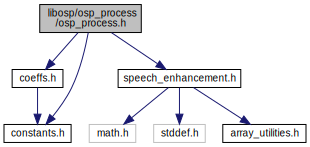
\includegraphics[width=350pt]{osp__process_8h__incl}
\end{center}
\end{figure}
This graph shows which files directly or indirectly include this file\+:\nopagebreak
\begin{figure}[H]
\begin{center}
\leavevmode
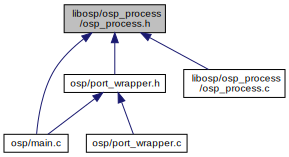
\includegraphics[width=350pt]{osp__process_8h__dep__incl}
\end{center}
\end{figure}
\subsection*{Functions}
\begin{DoxyCompactItemize}
\item 
int \mbox{\hyperlink{osp__process_8h_aabb5c0280f6d5cd0cce725a00533978f}{osp\+\_\+init}} (unsigned int frame\+\_\+size, int sample\+\_\+rate, \mbox{\hyperlink{constants_8h_a2d1d78531fe12807c3852488556d5a4b}{osp\+\_\+user\+\_\+data}} $\ast$osp\+\_\+data)
\begin{DoxyCompactList}\small\item\em This file groups all of the different O\+SP library calls in one place. This is more of an example way of using the different parts of the O\+SP libraries to implement a hearing aid algorith with M\+HA and A\+FC all in one place. \end{DoxyCompactList}\item 
void \mbox{\hyperlink{osp__process_8h_a6c8f16a08d0ce2a2b4989861253a51f5}{osp\+\_\+process\+\_\+audio}} (\mbox{\hyperlink{constants_8h_a2d1d78531fe12807c3852488556d5a4b}{osp\+\_\+user\+\_\+data}} $\ast$osp, float $\ast$x\+\_\+nL, float $\ast$x\+\_\+nR, float $\ast$outL, float $\ast$outR, size\+\_\+t len)
\begin{DoxyCompactList}\small\item\em Function to perform Master Hearing Aid (M\+HA) processing on the input signal for both channels. \end{DoxyCompactList}\item 
unsigned int \mbox{\hyperlink{osp__process_8h_afa87b8384a65fb6f6a12ac92297c9961}{osp\+\_\+get\+\_\+num\+\_\+bands}} ()
\begin{DoxyCompactList}\small\item\em Function to get the number of Sub-\/\+Bands. \end{DoxyCompactList}\item 
void \mbox{\hyperlink{osp__process_8h_af0a98853e0b3bce6a93cb88c1839723f}{osp\+\_\+close}} ()
\begin{DoxyCompactList}\small\item\em Wrapper function to free all the modules of Master Hearing Aid (M\+HA) \end{DoxyCompactList}\item 
void \mbox{\hyperlink{osp__process_8h_a37765f5c4d9ab3f3569947503b97a6c6}{osp\+\_\+dump\+\_\+afc\+\_\+filter}} ()
\begin{DoxyCompactList}\small\item\em Function to dump A\+FC filter taps for both left and right channels. \end{DoxyCompactList}\item 
void \mbox{\hyperlink{osp__process_8h_a12fc7be1c06d51523df05f460e91d097}{osp\+\_\+data\+\_\+init}} (\mbox{\hyperlink{constants_8h_a2d1d78531fe12807c3852488556d5a4b}{osp\+\_\+user\+\_\+data}} $\ast$user\+\_\+data)
\begin{DoxyCompactList}\small\item\em Helper function for initializing Master Hearing Aid (M\+HA) parameters. \end{DoxyCompactList}\item 
void \mbox{\hyperlink{osp__process_8h_a1b9e53a67adfda315e3fe93862361d22}{osp\+\_\+data\+\_\+set\+\_\+gain}} (\mbox{\hyperlink{constants_8h_a2d1d78531fe12807c3852488556d5a4b}{osp\+\_\+user\+\_\+data}} $\ast$user\+\_\+data, int gain)
\begin{DoxyCompactList}\small\item\em Helper function for initializing gain parameters for W\+D\+RC with a constant gain. \end{DoxyCompactList}\item 
void \mbox{\hyperlink{osp__process_8h_a6f9f5ada6b7f84af9827bbb1cbe68d3d}{osp\+\_\+data\+\_\+set\+\_\+nh}} (\mbox{\hyperlink{constants_8h_a2d1d78531fe12807c3852488556d5a4b}{osp\+\_\+user\+\_\+data}} $\ast$user\+\_\+data)
\begin{DoxyCompactList}\small\item\em Helper function for initializing gain parameters for W\+D\+RC with NH audiogram. \end{DoxyCompactList}\item 
void \mbox{\hyperlink{osp__process_8h_aa23c1072681c057f945a6d22d7659934}{osp\+\_\+data\+\_\+set\+\_\+n2}} (\mbox{\hyperlink{constants_8h_a2d1d78531fe12807c3852488556d5a4b}{osp\+\_\+user\+\_\+data}} $\ast$user\+\_\+data)
\begin{DoxyCompactList}\small\item\em Helper function for initializing gain parameters for W\+D\+RC with N2 audiogram. \end{DoxyCompactList}\item 
void \mbox{\hyperlink{osp__process_8h_ae7da3f44c97ca3e1ec342f2410015845}{osp\+\_\+data\+\_\+set\+\_\+n4}} (\mbox{\hyperlink{constants_8h_a2d1d78531fe12807c3852488556d5a4b}{osp\+\_\+user\+\_\+data}} $\ast$user\+\_\+data)
\begin{DoxyCompactList}\small\item\em Helper function for initializing gain parameters for W\+D\+RC with N4 audiogram. \end{DoxyCompactList}\item 
void \mbox{\hyperlink{osp__process_8h_aeb2474bd6b995d8ad289bfb1ce9b91c9}{osp\+\_\+data\+\_\+set\+\_\+s2}} (\mbox{\hyperlink{constants_8h_a2d1d78531fe12807c3852488556d5a4b}{osp\+\_\+user\+\_\+data}} $\ast$user\+\_\+data)
\begin{DoxyCompactList}\small\item\em Helper function for initializing gain parameters for W\+D\+RC with S2 audiogram. \end{DoxyCompactList}\end{DoxyCompactItemize}


\subsection{Function Documentation}
\mbox{\Hypertarget{osp__process_8h_af0a98853e0b3bce6a93cb88c1839723f}\label{osp__process_8h_af0a98853e0b3bce6a93cb88c1839723f}} 
\index{osp\+\_\+process.\+h@{osp\+\_\+process.\+h}!osp\+\_\+close@{osp\+\_\+close}}
\index{osp\+\_\+close@{osp\+\_\+close}!osp\+\_\+process.\+h@{osp\+\_\+process.\+h}}
\subsubsection{\texorpdfstring{osp\+\_\+close()}{osp\_close()}}
{\footnotesize\ttfamily void osp\+\_\+close (\begin{DoxyParamCaption}{ }\end{DoxyParamCaption})}



Wrapper function to free all the modules of Master Hearing Aid (M\+HA) 

\mbox{\Hypertarget{osp__process_8h_a12fc7be1c06d51523df05f460e91d097}\label{osp__process_8h_a12fc7be1c06d51523df05f460e91d097}} 
\index{osp\+\_\+process.\+h@{osp\+\_\+process.\+h}!osp\+\_\+data\+\_\+init@{osp\+\_\+data\+\_\+init}}
\index{osp\+\_\+data\+\_\+init@{osp\+\_\+data\+\_\+init}!osp\+\_\+process.\+h@{osp\+\_\+process.\+h}}
\subsubsection{\texorpdfstring{osp\+\_\+data\+\_\+init()}{osp\_data\_init()}}
{\footnotesize\ttfamily void osp\+\_\+data\+\_\+init (\begin{DoxyParamCaption}\item[{\mbox{\hyperlink{constants_8h_a2d1d78531fe12807c3852488556d5a4b}{osp\+\_\+user\+\_\+data}} $\ast$}]{user\+\_\+data }\end{DoxyParamCaption})}



Helper function for initializing Master Hearing Aid (M\+HA) parameters. 

\begin{DoxySeeAlso}{See also}
\mbox{\hyperlink{constants_8h_a2d1d78531fe12807c3852488556d5a4b}{osp\+\_\+user\+\_\+data}} 

\mbox{\hyperlink{osp__process_8h_a1b9e53a67adfda315e3fe93862361d22}{osp\+\_\+data\+\_\+set\+\_\+gain}}, \mbox{\hyperlink{osp__process_8h_a6f9f5ada6b7f84af9827bbb1cbe68d3d}{osp\+\_\+data\+\_\+set\+\_\+nh}}, \mbox{\hyperlink{osp__process_8h_aa23c1072681c057f945a6d22d7659934}{osp\+\_\+data\+\_\+set\+\_\+n2}} ,\mbox{\hyperlink{osp__process_8h_ae7da3f44c97ca3e1ec342f2410015845}{osp\+\_\+data\+\_\+set\+\_\+n4}} ,\mbox{\hyperlink{osp__process_8h_aeb2474bd6b995d8ad289bfb1ce9b91c9}{osp\+\_\+data\+\_\+set\+\_\+s2}} 
\end{DoxySeeAlso}

\begin{DoxyParams}{Parameters}
{\em user\+\_\+data} & Pointer to an osp\+\_\+user\+\_\+data instance which will be allocated in the function \\
\hline
\end{DoxyParams}
\mbox{\Hypertarget{osp__process_8h_a1b9e53a67adfda315e3fe93862361d22}\label{osp__process_8h_a1b9e53a67adfda315e3fe93862361d22}} 
\index{osp\+\_\+process.\+h@{osp\+\_\+process.\+h}!osp\+\_\+data\+\_\+set\+\_\+gain@{osp\+\_\+data\+\_\+set\+\_\+gain}}
\index{osp\+\_\+data\+\_\+set\+\_\+gain@{osp\+\_\+data\+\_\+set\+\_\+gain}!osp\+\_\+process.\+h@{osp\+\_\+process.\+h}}
\subsubsection{\texorpdfstring{osp\+\_\+data\+\_\+set\+\_\+gain()}{osp\_data\_set\_gain()}}
{\footnotesize\ttfamily void osp\+\_\+data\+\_\+set\+\_\+gain (\begin{DoxyParamCaption}\item[{\mbox{\hyperlink{constants_8h_a2d1d78531fe12807c3852488556d5a4b}{osp\+\_\+user\+\_\+data}} $\ast$}]{user\+\_\+data,  }\item[{int}]{gain }\end{DoxyParamCaption})}



Helper function for initializing gain parameters for W\+D\+RC with a constant gain. 

\begin{DoxySeeAlso}{See also}
\mbox{\hyperlink{constants_8h_a2d1d78531fe12807c3852488556d5a4b}{osp\+\_\+user\+\_\+data}} 

\mbox{\hyperlink{osp__process_8h_a1b9e53a67adfda315e3fe93862361d22}{osp\+\_\+data\+\_\+set\+\_\+gain}}, \mbox{\hyperlink{osp__process_8h_a6f9f5ada6b7f84af9827bbb1cbe68d3d}{osp\+\_\+data\+\_\+set\+\_\+nh}}, \mbox{\hyperlink{osp__process_8h_aa23c1072681c057f945a6d22d7659934}{osp\+\_\+data\+\_\+set\+\_\+n2}} ,\mbox{\hyperlink{osp__process_8h_ae7da3f44c97ca3e1ec342f2410015845}{osp\+\_\+data\+\_\+set\+\_\+n4}} ,\mbox{\hyperlink{osp__process_8h_aeb2474bd6b995d8ad289bfb1ce9b91c9}{osp\+\_\+data\+\_\+set\+\_\+s2}} 
\end{DoxySeeAlso}

\begin{DoxyParams}{Parameters}
{\em user\+\_\+data} & Pointer to the instance of osp\+\_\+user\+\_\+data initialized by osp\+\_\+data\+\_\+init \\
\hline
{\em gain} & The constant gain value \\
\hline
\end{DoxyParams}
\mbox{\Hypertarget{osp__process_8h_aa23c1072681c057f945a6d22d7659934}\label{osp__process_8h_aa23c1072681c057f945a6d22d7659934}} 
\index{osp\+\_\+process.\+h@{osp\+\_\+process.\+h}!osp\+\_\+data\+\_\+set\+\_\+n2@{osp\+\_\+data\+\_\+set\+\_\+n2}}
\index{osp\+\_\+data\+\_\+set\+\_\+n2@{osp\+\_\+data\+\_\+set\+\_\+n2}!osp\+\_\+process.\+h@{osp\+\_\+process.\+h}}
\subsubsection{\texorpdfstring{osp\+\_\+data\+\_\+set\+\_\+n2()}{osp\_data\_set\_n2()}}
{\footnotesize\ttfamily void osp\+\_\+data\+\_\+set\+\_\+n2 (\begin{DoxyParamCaption}\item[{\mbox{\hyperlink{constants_8h_a2d1d78531fe12807c3852488556d5a4b}{osp\+\_\+user\+\_\+data}} $\ast$}]{user\+\_\+data }\end{DoxyParamCaption})}



Helper function for initializing gain parameters for W\+D\+RC with N2 audiogram. 

\begin{DoxySeeAlso}{See also}
\mbox{\hyperlink{constants_8h_a2d1d78531fe12807c3852488556d5a4b}{osp\+\_\+user\+\_\+data}} 

\mbox{\hyperlink{osp__process_8h_a1b9e53a67adfda315e3fe93862361d22}{osp\+\_\+data\+\_\+set\+\_\+gain}}, \mbox{\hyperlink{osp__process_8h_a6f9f5ada6b7f84af9827bbb1cbe68d3d}{osp\+\_\+data\+\_\+set\+\_\+nh}}, \mbox{\hyperlink{osp__process_8h_aa23c1072681c057f945a6d22d7659934}{osp\+\_\+data\+\_\+set\+\_\+n2}} ,\mbox{\hyperlink{osp__process_8h_ae7da3f44c97ca3e1ec342f2410015845}{osp\+\_\+data\+\_\+set\+\_\+n4}} ,\mbox{\hyperlink{osp__process_8h_aeb2474bd6b995d8ad289bfb1ce9b91c9}{osp\+\_\+data\+\_\+set\+\_\+s2}} 
\end{DoxySeeAlso}

\begin{DoxyParams}{Parameters}
{\em user\+\_\+data} & Pointer to the instance of osp\+\_\+user\+\_\+data initialized by osp\+\_\+data\+\_\+init \\
\hline
\end{DoxyParams}
\mbox{\Hypertarget{osp__process_8h_ae7da3f44c97ca3e1ec342f2410015845}\label{osp__process_8h_ae7da3f44c97ca3e1ec342f2410015845}} 
\index{osp\+\_\+process.\+h@{osp\+\_\+process.\+h}!osp\+\_\+data\+\_\+set\+\_\+n4@{osp\+\_\+data\+\_\+set\+\_\+n4}}
\index{osp\+\_\+data\+\_\+set\+\_\+n4@{osp\+\_\+data\+\_\+set\+\_\+n4}!osp\+\_\+process.\+h@{osp\+\_\+process.\+h}}
\subsubsection{\texorpdfstring{osp\+\_\+data\+\_\+set\+\_\+n4()}{osp\_data\_set\_n4()}}
{\footnotesize\ttfamily void osp\+\_\+data\+\_\+set\+\_\+n4 (\begin{DoxyParamCaption}\item[{\mbox{\hyperlink{constants_8h_a2d1d78531fe12807c3852488556d5a4b}{osp\+\_\+user\+\_\+data}} $\ast$}]{user\+\_\+data }\end{DoxyParamCaption})}



Helper function for initializing gain parameters for W\+D\+RC with N4 audiogram. 

\begin{DoxySeeAlso}{See also}
\mbox{\hyperlink{constants_8h_a2d1d78531fe12807c3852488556d5a4b}{osp\+\_\+user\+\_\+data}} 

\mbox{\hyperlink{osp__process_8h_a1b9e53a67adfda315e3fe93862361d22}{osp\+\_\+data\+\_\+set\+\_\+gain}}, \mbox{\hyperlink{osp__process_8h_a6f9f5ada6b7f84af9827bbb1cbe68d3d}{osp\+\_\+data\+\_\+set\+\_\+nh}}, \mbox{\hyperlink{osp__process_8h_aa23c1072681c057f945a6d22d7659934}{osp\+\_\+data\+\_\+set\+\_\+n2}} ,\mbox{\hyperlink{osp__process_8h_ae7da3f44c97ca3e1ec342f2410015845}{osp\+\_\+data\+\_\+set\+\_\+n4}} ,\mbox{\hyperlink{osp__process_8h_aeb2474bd6b995d8ad289bfb1ce9b91c9}{osp\+\_\+data\+\_\+set\+\_\+s2}} 
\end{DoxySeeAlso}

\begin{DoxyParams}{Parameters}
{\em user\+\_\+data} & Pointer to the instance of osp\+\_\+user\+\_\+data initialized by osp\+\_\+data\+\_\+init \\
\hline
\end{DoxyParams}
\mbox{\Hypertarget{osp__process_8h_a6f9f5ada6b7f84af9827bbb1cbe68d3d}\label{osp__process_8h_a6f9f5ada6b7f84af9827bbb1cbe68d3d}} 
\index{osp\+\_\+process.\+h@{osp\+\_\+process.\+h}!osp\+\_\+data\+\_\+set\+\_\+nh@{osp\+\_\+data\+\_\+set\+\_\+nh}}
\index{osp\+\_\+data\+\_\+set\+\_\+nh@{osp\+\_\+data\+\_\+set\+\_\+nh}!osp\+\_\+process.\+h@{osp\+\_\+process.\+h}}
\subsubsection{\texorpdfstring{osp\+\_\+data\+\_\+set\+\_\+nh()}{osp\_data\_set\_nh()}}
{\footnotesize\ttfamily void osp\+\_\+data\+\_\+set\+\_\+nh (\begin{DoxyParamCaption}\item[{\mbox{\hyperlink{constants_8h_a2d1d78531fe12807c3852488556d5a4b}{osp\+\_\+user\+\_\+data}} $\ast$}]{user\+\_\+data }\end{DoxyParamCaption})}



Helper function for initializing gain parameters for W\+D\+RC with NH audiogram. 

\begin{DoxySeeAlso}{See also}
\mbox{\hyperlink{constants_8h_a2d1d78531fe12807c3852488556d5a4b}{osp\+\_\+user\+\_\+data}} 

\mbox{\hyperlink{osp__process_8h_a1b9e53a67adfda315e3fe93862361d22}{osp\+\_\+data\+\_\+set\+\_\+gain}}, \mbox{\hyperlink{osp__process_8h_a6f9f5ada6b7f84af9827bbb1cbe68d3d}{osp\+\_\+data\+\_\+set\+\_\+nh}}, \mbox{\hyperlink{osp__process_8h_aa23c1072681c057f945a6d22d7659934}{osp\+\_\+data\+\_\+set\+\_\+n2}} ,\mbox{\hyperlink{osp__process_8h_ae7da3f44c97ca3e1ec342f2410015845}{osp\+\_\+data\+\_\+set\+\_\+n4}} ,\mbox{\hyperlink{osp__process_8h_aeb2474bd6b995d8ad289bfb1ce9b91c9}{osp\+\_\+data\+\_\+set\+\_\+s2}} 
\end{DoxySeeAlso}

\begin{DoxyParams}{Parameters}
{\em user\+\_\+data} & Pointer to the instance of osp\+\_\+user\+\_\+data initialized by osp\+\_\+data\+\_\+init \\
\hline
\end{DoxyParams}
\mbox{\Hypertarget{osp__process_8h_aeb2474bd6b995d8ad289bfb1ce9b91c9}\label{osp__process_8h_aeb2474bd6b995d8ad289bfb1ce9b91c9}} 
\index{osp\+\_\+process.\+h@{osp\+\_\+process.\+h}!osp\+\_\+data\+\_\+set\+\_\+s2@{osp\+\_\+data\+\_\+set\+\_\+s2}}
\index{osp\+\_\+data\+\_\+set\+\_\+s2@{osp\+\_\+data\+\_\+set\+\_\+s2}!osp\+\_\+process.\+h@{osp\+\_\+process.\+h}}
\subsubsection{\texorpdfstring{osp\+\_\+data\+\_\+set\+\_\+s2()}{osp\_data\_set\_s2()}}
{\footnotesize\ttfamily void osp\+\_\+data\+\_\+set\+\_\+s2 (\begin{DoxyParamCaption}\item[{\mbox{\hyperlink{constants_8h_a2d1d78531fe12807c3852488556d5a4b}{osp\+\_\+user\+\_\+data}} $\ast$}]{user\+\_\+data }\end{DoxyParamCaption})}



Helper function for initializing gain parameters for W\+D\+RC with S2 audiogram. 

\begin{DoxySeeAlso}{See also}
\mbox{\hyperlink{constants_8h_a2d1d78531fe12807c3852488556d5a4b}{osp\+\_\+user\+\_\+data}} 

\mbox{\hyperlink{osp__process_8h_a1b9e53a67adfda315e3fe93862361d22}{osp\+\_\+data\+\_\+set\+\_\+gain}}, \mbox{\hyperlink{osp__process_8h_a6f9f5ada6b7f84af9827bbb1cbe68d3d}{osp\+\_\+data\+\_\+set\+\_\+nh}}, \mbox{\hyperlink{osp__process_8h_aa23c1072681c057f945a6d22d7659934}{osp\+\_\+data\+\_\+set\+\_\+n2}} ,\mbox{\hyperlink{osp__process_8h_ae7da3f44c97ca3e1ec342f2410015845}{osp\+\_\+data\+\_\+set\+\_\+n4}} ,\mbox{\hyperlink{osp__process_8h_aeb2474bd6b995d8ad289bfb1ce9b91c9}{osp\+\_\+data\+\_\+set\+\_\+s2}} 
\end{DoxySeeAlso}

\begin{DoxyParams}{Parameters}
{\em user\+\_\+data} & Pointer to the instance of osp\+\_\+user\+\_\+data initialized by osp\+\_\+data\+\_\+init \\
\hline
\end{DoxyParams}
\mbox{\Hypertarget{osp__process_8h_a37765f5c4d9ab3f3569947503b97a6c6}\label{osp__process_8h_a37765f5c4d9ab3f3569947503b97a6c6}} 
\index{osp\+\_\+process.\+h@{osp\+\_\+process.\+h}!osp\+\_\+dump\+\_\+afc\+\_\+filter@{osp\+\_\+dump\+\_\+afc\+\_\+filter}}
\index{osp\+\_\+dump\+\_\+afc\+\_\+filter@{osp\+\_\+dump\+\_\+afc\+\_\+filter}!osp\+\_\+process.\+h@{osp\+\_\+process.\+h}}
\subsubsection{\texorpdfstring{osp\+\_\+dump\+\_\+afc\+\_\+filter()}{osp\_dump\_afc\_filter()}}
{\footnotesize\ttfamily void osp\+\_\+dump\+\_\+afc\+\_\+filter (\begin{DoxyParamCaption}{ }\end{DoxyParamCaption})}



Function to dump A\+FC filter taps for both left and right channels. 

File names can be changed by changing A\+F\+C\+\_\+\+F\+I\+L\+T\+E\+R\+\_\+\+T\+A\+P\+\_\+\+F\+I\+L\+E\+\_\+L, A\+F\+C\+\_\+\+F\+I\+L\+T\+E\+R\+\_\+\+T\+A\+P\+\_\+\+F\+I\+L\+E\+\_\+R in \mbox{\hyperlink{constants_8h}{constants.\+h}} \mbox{\Hypertarget{osp__process_8h_afa87b8384a65fb6f6a12ac92297c9961}\label{osp__process_8h_afa87b8384a65fb6f6a12ac92297c9961}} 
\index{osp\+\_\+process.\+h@{osp\+\_\+process.\+h}!osp\+\_\+get\+\_\+num\+\_\+bands@{osp\+\_\+get\+\_\+num\+\_\+bands}}
\index{osp\+\_\+get\+\_\+num\+\_\+bands@{osp\+\_\+get\+\_\+num\+\_\+bands}!osp\+\_\+process.\+h@{osp\+\_\+process.\+h}}
\subsubsection{\texorpdfstring{osp\+\_\+get\+\_\+num\+\_\+bands()}{osp\_get\_num\_bands()}}
{\footnotesize\ttfamily unsigned int osp\+\_\+get\+\_\+num\+\_\+bands (\begin{DoxyParamCaption}{ }\end{DoxyParamCaption})}



Function to get the number of Sub-\/\+Bands. 

\begin{DoxyReturn}{Returns}
int Number of Sub-\/\+Bands give by N\+U\+M\+\_\+\+B\+A\+N\+DS 
\end{DoxyReturn}
\mbox{\Hypertarget{osp__process_8h_aabb5c0280f6d5cd0cce725a00533978f}\label{osp__process_8h_aabb5c0280f6d5cd0cce725a00533978f}} 
\index{osp\+\_\+process.\+h@{osp\+\_\+process.\+h}!osp\+\_\+init@{osp\+\_\+init}}
\index{osp\+\_\+init@{osp\+\_\+init}!osp\+\_\+process.\+h@{osp\+\_\+process.\+h}}
\subsubsection{\texorpdfstring{osp\+\_\+init()}{osp\_init()}}
{\footnotesize\ttfamily int osp\+\_\+init (\begin{DoxyParamCaption}\item[{unsigned int}]{frame\+\_\+size,  }\item[{int}]{sample\+\_\+rate,  }\item[{\mbox{\hyperlink{constants_8h_a2d1d78531fe12807c3852488556d5a4b}{osp\+\_\+user\+\_\+data}} $\ast$}]{osp\+\_\+data }\end{DoxyParamCaption})}



This file groups all of the different O\+SP library calls in one place. This is more of an example way of using the different parts of the O\+SP libraries to implement a hearing aid algorith with M\+HA and A\+FC all in one place. 

Wrapper function to initalize all the modules of Master Hearing Aid (M\+HA)


\begin{DoxyParams}{Parameters}
{\em frame\+\_\+size} & The number of samples in a frame. i.\+e. the number of samples to process \\
\hline
{\em sample\+\_\+rate} & The sample rate at which all M\+HA processing will be done \\
\hline
{\em afc\+\_\+adaptation\+\_\+type} & The type of A\+FC adaptation \\
\hline
\end{DoxyParams}
\begin{DoxyReturn}{Returns}
0 if successful initialization. -\/1 otherwise 
\end{DoxyReturn}
\mbox{\Hypertarget{osp__process_8h_a6c8f16a08d0ce2a2b4989861253a51f5}\label{osp__process_8h_a6c8f16a08d0ce2a2b4989861253a51f5}} 
\index{osp\+\_\+process.\+h@{osp\+\_\+process.\+h}!osp\+\_\+process\+\_\+audio@{osp\+\_\+process\+\_\+audio}}
\index{osp\+\_\+process\+\_\+audio@{osp\+\_\+process\+\_\+audio}!osp\+\_\+process.\+h@{osp\+\_\+process.\+h}}
\subsubsection{\texorpdfstring{osp\+\_\+process\+\_\+audio()}{osp\_process\_audio()}}
{\footnotesize\ttfamily void osp\+\_\+process\+\_\+audio (\begin{DoxyParamCaption}\item[{\mbox{\hyperlink{constants_8h_a2d1d78531fe12807c3852488556d5a4b}{osp\+\_\+user\+\_\+data}} $\ast$}]{osp,  }\item[{float $\ast$}]{x\+\_\+nL,  }\item[{float $\ast$}]{x\+\_\+nR,  }\item[{float $\ast$}]{outL,  }\item[{float $\ast$}]{outR,  }\item[{size\+\_\+t}]{len }\end{DoxyParamCaption})}



Function to perform Master Hearing Aid (M\+HA) processing on the input signal for both channels. 

If S\+T\+E\+R\+EO is false, only the right channel is processed

\begin{DoxySeeAlso}{See also}
\mbox{\hyperlink{constants_8h_a2d1d78531fe12807c3852488556d5a4b}{osp\+\_\+user\+\_\+data}} 
\end{DoxySeeAlso}

\begin{DoxyParams}{Parameters}
{\em osp} & The instance of the osp\+\_\+user\+\_\+data structure that was initialized in osp\+\_\+data\+\_\+init. This contains all the M\+HA parameters. \\
\hline
{\em x\+\_\+nL} & Pointer to the array containing left channel input \\
\hline
{\em x\+\_\+nR} & Pointer to the array containing right channel input \\
\hline
{\em outL} & Pointer to the array to store the output of M\+HA processing on left channel input \\
\hline
{\em outR} & Pointer to the array to store the output of M\+HA processing on right channel input \\
\hline
{\em len} & The length of the input signal e\+\_\+n that is given for processing. i.\+e. frame length. \\
\hline
\end{DoxyParams}

\hypertarget{utilities_8c}{}\section{libosp/osp\+\_\+process/utilities.c File Reference}
\label{utilities_8c}\index{libosp/osp\+\_\+process/utilities.\+c@{libosp/osp\+\_\+process/utilities.\+c}}
{\ttfamily \#include $<$stdio.\+h$>$}\newline
{\ttfamily \#include $<$stdlib.\+h$>$}\newline
{\ttfamily \#include $<$limits.\+h$>$}\newline
Include dependency graph for utilities.\+c\+:\nopagebreak
\begin{figure}[H]
\begin{center}
\leavevmode
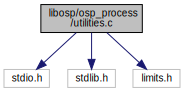
\includegraphics[width=256pt]{utilities_8c__incl}
\end{center}
\end{figure}
\subsection*{Functions}
\begin{DoxyCompactItemize}
\item 
int \mbox{\hyperlink{utilities_8c_aa884370487e6a35d482982274134a94c}{load\+\_\+filter\+\_\+taps}} (const char $\ast$file, float $\ast$taps, int len)
\begin{DoxyCompactList}\small\item\em Load filter taps from file. \end{DoxyCompactList}\item 
int \mbox{\hyperlink{utilities_8c_a11a85d9e5da9385c325c40be7f393284}{save\+\_\+filter\+\_\+taps}} (const char $\ast$file, float $\ast$taps, int len)
\begin{DoxyCompactList}\small\item\em Save filter taps to a file. \end{DoxyCompactList}\end{DoxyCompactItemize}


\subsection{Function Documentation}
\mbox{\Hypertarget{utilities_8c_aa884370487e6a35d482982274134a94c}\label{utilities_8c_aa884370487e6a35d482982274134a94c}} 
\index{utilities.\+c@{utilities.\+c}!load\+\_\+filter\+\_\+taps@{load\+\_\+filter\+\_\+taps}}
\index{load\+\_\+filter\+\_\+taps@{load\+\_\+filter\+\_\+taps}!utilities.\+c@{utilities.\+c}}
\subsubsection{\texorpdfstring{load\+\_\+filter\+\_\+taps()}{load\_filter\_taps()}}
{\footnotesize\ttfamily int load\+\_\+filter\+\_\+taps (\begin{DoxyParamCaption}\item[{const char $\ast$}]{file,  }\item[{float $\ast$}]{taps,  }\item[{int}]{len }\end{DoxyParamCaption})}



Load filter taps from file. 


\begin{DoxyParams}{Parameters}
{\em file} & The file in which to load 32bit float taps from \\
\hline
{\em taps} & The array in which the taps will be loaded into \\
\hline
{\em len} & The number of taps to load into the \char`\"{}taps\char`\"{} array\\
\hline
\end{DoxyParams}
\begin{DoxyReturn}{Returns}
Returns the number of taps loaded. This should be the same as the \char`\"{}len\char`\"{} parameter. This way the developer can test if this is the case, and return an error if it is not 
\end{DoxyReturn}
\mbox{\Hypertarget{utilities_8c_a11a85d9e5da9385c325c40be7f393284}\label{utilities_8c_a11a85d9e5da9385c325c40be7f393284}} 
\index{utilities.\+c@{utilities.\+c}!save\+\_\+filter\+\_\+taps@{save\+\_\+filter\+\_\+taps}}
\index{save\+\_\+filter\+\_\+taps@{save\+\_\+filter\+\_\+taps}!utilities.\+c@{utilities.\+c}}
\subsubsection{\texorpdfstring{save\+\_\+filter\+\_\+taps()}{save\_filter\_taps()}}
{\footnotesize\ttfamily int save\+\_\+filter\+\_\+taps (\begin{DoxyParamCaption}\item[{const char $\ast$}]{file,  }\item[{float $\ast$}]{taps,  }\item[{int}]{len }\end{DoxyParamCaption})}



Save filter taps to a file. 


\begin{DoxyParams}{Parameters}
{\em file} & File to save filter taps to \\
\hline
{\em taps} & Array of filter taps to save to file \\
\hline
{\em len} & Length of the \char`\"{}taps\char`\"{} array\+: the number of taps to save\\
\hline
\end{DoxyParams}
\begin{DoxyReturn}{Returns}
Returns 0 on success, -\/1 otherwise 
\end{DoxyReturn}

\hypertarget{utilities_8h}{}\section{libosp/osp\+\_\+process/utilities.h File Reference}
\label{utilities_8h}\index{libosp/osp\+\_\+process/utilities.\+h@{libosp/osp\+\_\+process/utilities.\+h}}
This graph shows which files directly or indirectly include this file\+:\nopagebreak
\begin{figure}[H]
\begin{center}
\leavevmode
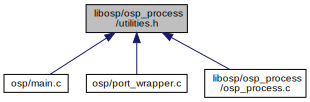
\includegraphics[width=350pt]{utilities_8h__dep__incl}
\end{center}
\end{figure}
\subsection*{Macros}
\begin{DoxyCompactItemize}
\item 
\#define \mbox{\hyperlink{utilities_8h_a6242a25f9d996f0cc4f4cdb911218b75}{A\+R\+R\+A\+Y\+\_\+\+S\+I\+ZE}}(x)~(sizeof((x)) / sizeof((x)\mbox{[}0\mbox{]}))
\end{DoxyCompactItemize}
\subsection*{Functions}
\begin{DoxyCompactItemize}
\item 
int \mbox{\hyperlink{utilities_8h_aa884370487e6a35d482982274134a94c}{load\+\_\+filter\+\_\+taps}} (const char $\ast$file, float $\ast$taps, int len)
\begin{DoxyCompactList}\small\item\em Load filter taps from file. \end{DoxyCompactList}\item 
int \mbox{\hyperlink{utilities_8h_a11a85d9e5da9385c325c40be7f393284}{save\+\_\+filter\+\_\+taps}} (const char $\ast$file, float $\ast$taps, int len)
\begin{DoxyCompactList}\small\item\em Save filter taps to a file. \end{DoxyCompactList}\end{DoxyCompactItemize}


\subsection{Macro Definition Documentation}
\mbox{\Hypertarget{utilities_8h_a6242a25f9d996f0cc4f4cdb911218b75}\label{utilities_8h_a6242a25f9d996f0cc4f4cdb911218b75}} 
\index{utilities.\+h@{utilities.\+h}!A\+R\+R\+A\+Y\+\_\+\+S\+I\+ZE@{A\+R\+R\+A\+Y\+\_\+\+S\+I\+ZE}}
\index{A\+R\+R\+A\+Y\+\_\+\+S\+I\+ZE@{A\+R\+R\+A\+Y\+\_\+\+S\+I\+ZE}!utilities.\+h@{utilities.\+h}}
\subsubsection{\texorpdfstring{A\+R\+R\+A\+Y\+\_\+\+S\+I\+ZE}{ARRAY\_SIZE}}
{\footnotesize\ttfamily \#define A\+R\+R\+A\+Y\+\_\+\+S\+I\+ZE(\begin{DoxyParamCaption}\item[{}]{x }\end{DoxyParamCaption})~(sizeof((x)) / sizeof((x)\mbox{[}0\mbox{]}))}



\subsection{Function Documentation}
\mbox{\Hypertarget{utilities_8h_aa884370487e6a35d482982274134a94c}\label{utilities_8h_aa884370487e6a35d482982274134a94c}} 
\index{utilities.\+h@{utilities.\+h}!load\+\_\+filter\+\_\+taps@{load\+\_\+filter\+\_\+taps}}
\index{load\+\_\+filter\+\_\+taps@{load\+\_\+filter\+\_\+taps}!utilities.\+h@{utilities.\+h}}
\subsubsection{\texorpdfstring{load\+\_\+filter\+\_\+taps()}{load\_filter\_taps()}}
{\footnotesize\ttfamily int load\+\_\+filter\+\_\+taps (\begin{DoxyParamCaption}\item[{const char $\ast$}]{file,  }\item[{float $\ast$}]{taps,  }\item[{int}]{len }\end{DoxyParamCaption})}



Load filter taps from file. 


\begin{DoxyParams}{Parameters}
{\em file} & The file in which to load 32bit float taps from \\
\hline
{\em taps} & The array in which the taps will be loaded into \\
\hline
{\em len} & The number of taps to load into the \char`\"{}taps\char`\"{} array\\
\hline
\end{DoxyParams}
\begin{DoxyReturn}{Returns}
Returns the number of taps loaded. This should be the same as the \char`\"{}len\char`\"{} parameter. This way the developer can test if this is the case, and return an error if it is not 
\end{DoxyReturn}
\mbox{\Hypertarget{utilities_8h_a11a85d9e5da9385c325c40be7f393284}\label{utilities_8h_a11a85d9e5da9385c325c40be7f393284}} 
\index{utilities.\+h@{utilities.\+h}!save\+\_\+filter\+\_\+taps@{save\+\_\+filter\+\_\+taps}}
\index{save\+\_\+filter\+\_\+taps@{save\+\_\+filter\+\_\+taps}!utilities.\+h@{utilities.\+h}}
\subsubsection{\texorpdfstring{save\+\_\+filter\+\_\+taps()}{save\_filter\_taps()}}
{\footnotesize\ttfamily int save\+\_\+filter\+\_\+taps (\begin{DoxyParamCaption}\item[{const char $\ast$}]{file,  }\item[{float $\ast$}]{taps,  }\item[{int}]{len }\end{DoxyParamCaption})}



Save filter taps to a file. 


\begin{DoxyParams}{Parameters}
{\em file} & File to save filter taps to \\
\hline
{\em taps} & Array of filter taps to save to file \\
\hline
{\em len} & Length of the \char`\"{}taps\char`\"{} array\+: the number of taps to save\\
\hline
\end{DoxyParams}
\begin{DoxyReturn}{Returns}
Returns 0 on success, -\/1 otherwise 
\end{DoxyReturn}

\hypertarget{jsmn_8c}{}\section{libosp/osp\+\_\+tcp/json\+\_\+parser/jsmn.c File Reference}
\label{jsmn_8c}\index{libosp/osp\+\_\+tcp/json\+\_\+parser/jsmn.\+c@{libosp/osp\+\_\+tcp/json\+\_\+parser/jsmn.\+c}}
{\ttfamily \#include \char`\"{}jsmn.\+h\char`\"{}}\newline
Include dependency graph for jsmn.\+c\+:\nopagebreak
\begin{figure}[H]
\begin{center}
\leavevmode
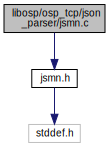
\includegraphics[width=181pt]{jsmn_8c__incl}
\end{center}
\end{figure}
\subsection*{Functions}
\begin{DoxyCompactItemize}
\item 
static \mbox{\hyperlink{structjsmntok__t}{jsmntok\+\_\+t}} $\ast$ \mbox{\hyperlink{jsmn_8c_a0d7a964b95b65cd16699a355ede80394}{jsmn\+\_\+alloc\+\_\+token}} (\mbox{\hyperlink{structjsmn__parser}{jsmn\+\_\+parser}} $\ast$parser, \mbox{\hyperlink{structjsmntok__t}{jsmntok\+\_\+t}} $\ast$tokens, size\+\_\+t num\+\_\+tokens)
\item 
static void \mbox{\hyperlink{jsmn_8c_a20b875e37a2a5c88888c6d80068715be}{jsmn\+\_\+fill\+\_\+token}} (\mbox{\hyperlink{structjsmntok__t}{jsmntok\+\_\+t}} $\ast$token, \mbox{\hyperlink{jsmn_8h_a065320719769f9dc1fbe30094e52802f}{jsmntype\+\_\+t}} type, int start, int end)
\item 
static int \mbox{\hyperlink{jsmn_8c_a4d1f29464811e2bbf5506fbe5c7ee9de}{jsmn\+\_\+parse\+\_\+primitive}} (\mbox{\hyperlink{structjsmn__parser}{jsmn\+\_\+parser}} $\ast$parser, const char $\ast$js, size\+\_\+t len, \mbox{\hyperlink{structjsmntok__t}{jsmntok\+\_\+t}} $\ast$tokens, size\+\_\+t num\+\_\+tokens)
\item 
static int \mbox{\hyperlink{jsmn_8c_a568f184e45bb9718270088e1e05a4264}{jsmn\+\_\+parse\+\_\+string}} (\mbox{\hyperlink{structjsmn__parser}{jsmn\+\_\+parser}} $\ast$parser, const char $\ast$js, size\+\_\+t len, \mbox{\hyperlink{structjsmntok__t}{jsmntok\+\_\+t}} $\ast$tokens, size\+\_\+t num\+\_\+tokens)
\item 
int \mbox{\hyperlink{jsmn_8c_a774f985a9750a10c7e88304e30191e03}{jsmn\+\_\+parse}} (\mbox{\hyperlink{structjsmn__parser}{jsmn\+\_\+parser}} $\ast$parser, const char $\ast$js, size\+\_\+t len, \mbox{\hyperlink{structjsmntok__t}{jsmntok\+\_\+t}} $\ast$tokens, unsigned int num\+\_\+tokens)
\item 
void \mbox{\hyperlink{jsmn_8c_a8d4a8b3ce5c3d600feea38615b5f9aa6}{jsmn\+\_\+init}} (\mbox{\hyperlink{structjsmn__parser}{jsmn\+\_\+parser}} $\ast$parser)
\end{DoxyCompactItemize}


\subsection{Function Documentation}
\mbox{\Hypertarget{jsmn_8c_a0d7a964b95b65cd16699a355ede80394}\label{jsmn_8c_a0d7a964b95b65cd16699a355ede80394}} 
\index{jsmn.\+c@{jsmn.\+c}!jsmn\+\_\+alloc\+\_\+token@{jsmn\+\_\+alloc\+\_\+token}}
\index{jsmn\+\_\+alloc\+\_\+token@{jsmn\+\_\+alloc\+\_\+token}!jsmn.\+c@{jsmn.\+c}}
\subsubsection{\texorpdfstring{jsmn\+\_\+alloc\+\_\+token()}{jsmn\_alloc\_token()}}
{\footnotesize\ttfamily static \mbox{\hyperlink{structjsmntok__t}{jsmntok\+\_\+t}}$\ast$ jsmn\+\_\+alloc\+\_\+token (\begin{DoxyParamCaption}\item[{\mbox{\hyperlink{structjsmn__parser}{jsmn\+\_\+parser}} $\ast$}]{parser,  }\item[{\mbox{\hyperlink{structjsmntok__t}{jsmntok\+\_\+t}} $\ast$}]{tokens,  }\item[{size\+\_\+t}]{num\+\_\+tokens }\end{DoxyParamCaption})\hspace{0.3cm}{\ttfamily [static]}}

Allocates a fresh unused token from the token pull. \mbox{\Hypertarget{jsmn_8c_a20b875e37a2a5c88888c6d80068715be}\label{jsmn_8c_a20b875e37a2a5c88888c6d80068715be}} 
\index{jsmn.\+c@{jsmn.\+c}!jsmn\+\_\+fill\+\_\+token@{jsmn\+\_\+fill\+\_\+token}}
\index{jsmn\+\_\+fill\+\_\+token@{jsmn\+\_\+fill\+\_\+token}!jsmn.\+c@{jsmn.\+c}}
\subsubsection{\texorpdfstring{jsmn\+\_\+fill\+\_\+token()}{jsmn\_fill\_token()}}
{\footnotesize\ttfamily static void jsmn\+\_\+fill\+\_\+token (\begin{DoxyParamCaption}\item[{\mbox{\hyperlink{structjsmntok__t}{jsmntok\+\_\+t}} $\ast$}]{token,  }\item[{\mbox{\hyperlink{jsmn_8h_a065320719769f9dc1fbe30094e52802f}{jsmntype\+\_\+t}}}]{type,  }\item[{int}]{start,  }\item[{int}]{end }\end{DoxyParamCaption})\hspace{0.3cm}{\ttfamily [static]}}

Fills token type and boundaries. \mbox{\Hypertarget{jsmn_8c_a8d4a8b3ce5c3d600feea38615b5f9aa6}\label{jsmn_8c_a8d4a8b3ce5c3d600feea38615b5f9aa6}} 
\index{jsmn.\+c@{jsmn.\+c}!jsmn\+\_\+init@{jsmn\+\_\+init}}
\index{jsmn\+\_\+init@{jsmn\+\_\+init}!jsmn.\+c@{jsmn.\+c}}
\subsubsection{\texorpdfstring{jsmn\+\_\+init()}{jsmn\_init()}}
{\footnotesize\ttfamily void jsmn\+\_\+init (\begin{DoxyParamCaption}\item[{\mbox{\hyperlink{structjsmn__parser}{jsmn\+\_\+parser}} $\ast$}]{parser }\end{DoxyParamCaption})}

Creates a new parser based over a given buffer with an array of tokens available. \mbox{\Hypertarget{jsmn_8c_a774f985a9750a10c7e88304e30191e03}\label{jsmn_8c_a774f985a9750a10c7e88304e30191e03}} 
\index{jsmn.\+c@{jsmn.\+c}!jsmn\+\_\+parse@{jsmn\+\_\+parse}}
\index{jsmn\+\_\+parse@{jsmn\+\_\+parse}!jsmn.\+c@{jsmn.\+c}}
\subsubsection{\texorpdfstring{jsmn\+\_\+parse()}{jsmn\_parse()}}
{\footnotesize\ttfamily int jsmn\+\_\+parse (\begin{DoxyParamCaption}\item[{\mbox{\hyperlink{structjsmn__parser}{jsmn\+\_\+parser}} $\ast$}]{parser,  }\item[{const char $\ast$}]{js,  }\item[{size\+\_\+t}]{len,  }\item[{\mbox{\hyperlink{structjsmntok__t}{jsmntok\+\_\+t}} $\ast$}]{tokens,  }\item[{unsigned int}]{num\+\_\+tokens }\end{DoxyParamCaption})}

Parse J\+S\+ON string and fill tokens. \mbox{\Hypertarget{jsmn_8c_a4d1f29464811e2bbf5506fbe5c7ee9de}\label{jsmn_8c_a4d1f29464811e2bbf5506fbe5c7ee9de}} 
\index{jsmn.\+c@{jsmn.\+c}!jsmn\+\_\+parse\+\_\+primitive@{jsmn\+\_\+parse\+\_\+primitive}}
\index{jsmn\+\_\+parse\+\_\+primitive@{jsmn\+\_\+parse\+\_\+primitive}!jsmn.\+c@{jsmn.\+c}}
\subsubsection{\texorpdfstring{jsmn\+\_\+parse\+\_\+primitive()}{jsmn\_parse\_primitive()}}
{\footnotesize\ttfamily static int jsmn\+\_\+parse\+\_\+primitive (\begin{DoxyParamCaption}\item[{\mbox{\hyperlink{structjsmn__parser}{jsmn\+\_\+parser}} $\ast$}]{parser,  }\item[{const char $\ast$}]{js,  }\item[{size\+\_\+t}]{len,  }\item[{\mbox{\hyperlink{structjsmntok__t}{jsmntok\+\_\+t}} $\ast$}]{tokens,  }\item[{size\+\_\+t}]{num\+\_\+tokens }\end{DoxyParamCaption})\hspace{0.3cm}{\ttfamily [static]}}

Fills next available token with J\+S\+ON primitive. \mbox{\Hypertarget{jsmn_8c_a568f184e45bb9718270088e1e05a4264}\label{jsmn_8c_a568f184e45bb9718270088e1e05a4264}} 
\index{jsmn.\+c@{jsmn.\+c}!jsmn\+\_\+parse\+\_\+string@{jsmn\+\_\+parse\+\_\+string}}
\index{jsmn\+\_\+parse\+\_\+string@{jsmn\+\_\+parse\+\_\+string}!jsmn.\+c@{jsmn.\+c}}
\subsubsection{\texorpdfstring{jsmn\+\_\+parse\+\_\+string()}{jsmn\_parse\_string()}}
{\footnotesize\ttfamily static int jsmn\+\_\+parse\+\_\+string (\begin{DoxyParamCaption}\item[{\mbox{\hyperlink{structjsmn__parser}{jsmn\+\_\+parser}} $\ast$}]{parser,  }\item[{const char $\ast$}]{js,  }\item[{size\+\_\+t}]{len,  }\item[{\mbox{\hyperlink{structjsmntok__t}{jsmntok\+\_\+t}} $\ast$}]{tokens,  }\item[{size\+\_\+t}]{num\+\_\+tokens }\end{DoxyParamCaption})\hspace{0.3cm}{\ttfamily [static]}}

Fills next token with J\+S\+ON string. 
\hypertarget{jsmn_8h}{}\section{libosp/osp\+\_\+tcp/json\+\_\+parser/jsmn.h File Reference}
\label{jsmn_8h}\index{libosp/osp\+\_\+tcp/json\+\_\+parser/jsmn.\+h@{libosp/osp\+\_\+tcp/json\+\_\+parser/jsmn.\+h}}
{\ttfamily \#include $<$stddef.\+h$>$}\newline
Include dependency graph for jsmn.\+h\+:\nopagebreak
\begin{figure}[H]
\begin{center}
\leavevmode
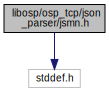
\includegraphics[width=181pt]{jsmn_8h__incl}
\end{center}
\end{figure}
This graph shows which files directly or indirectly include this file\+:\nopagebreak
\begin{figure}[H]
\begin{center}
\leavevmode
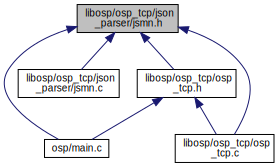
\includegraphics[width=350pt]{jsmn_8h__dep__incl}
\end{center}
\end{figure}
\subsection*{Data Structures}
\begin{DoxyCompactItemize}
\item 
struct \mbox{\hyperlink{structjsmntok__t}{jsmntok\+\_\+t}}
\item 
struct \mbox{\hyperlink{structjsmn__parser}{jsmn\+\_\+parser}}
\end{DoxyCompactItemize}
\subsection*{Enumerations}
\begin{DoxyCompactItemize}
\item 
enum \mbox{\hyperlink{jsmn_8h_a065320719769f9dc1fbe30094e52802f}{jsmntype\+\_\+t}} \{ \newline
\mbox{\hyperlink{jsmn_8h_a065320719769f9dc1fbe30094e52802fa7bc5faeddd33197250cf352af984f185}{J\+S\+M\+N\+\_\+\+U\+N\+D\+E\+F\+I\+N\+ED}} = 0, 
\mbox{\hyperlink{jsmn_8h_a065320719769f9dc1fbe30094e52802fa416d6e733082bedc1166f0d66f571867}{J\+S\+M\+N\+\_\+\+O\+B\+J\+E\+CT}} = 1, 
\mbox{\hyperlink{jsmn_8h_a065320719769f9dc1fbe30094e52802fabc4c47216dacf36bd4f64ac3d649d471}{J\+S\+M\+N\+\_\+\+A\+R\+R\+AY}} = 2, 
\mbox{\hyperlink{jsmn_8h_a065320719769f9dc1fbe30094e52802fad4ea6277c135d9d3377bf8b719779539}{J\+S\+M\+N\+\_\+\+S\+T\+R\+I\+NG}} = 3, 
\newline
\mbox{\hyperlink{jsmn_8h_a065320719769f9dc1fbe30094e52802fa2550c93fe929f81f30ea9b629ed98742}{J\+S\+M\+N\+\_\+\+P\+R\+I\+M\+I\+T\+I\+VE}} = 4
 \}
\item 
enum \mbox{\hyperlink{jsmn_8h_afbbe22e63007677ec9e7837b5c1b80ea}{jsmnerr}} \{ \mbox{\hyperlink{jsmn_8h_afbbe22e63007677ec9e7837b5c1b80eaafa350a2c19cc5fddbfb7c90309d3fe41}{J\+S\+M\+N\+\_\+\+E\+R\+R\+O\+R\+\_\+\+N\+O\+M\+EM}} = -\/1, 
\mbox{\hyperlink{jsmn_8h_afbbe22e63007677ec9e7837b5c1b80eaa3297b1c54d926ce497b7a20530689171}{J\+S\+M\+N\+\_\+\+E\+R\+R\+O\+R\+\_\+\+I\+N\+V\+AL}} = -\/2, 
\mbox{\hyperlink{jsmn_8h_afbbe22e63007677ec9e7837b5c1b80eaa851a0e75343c14a13c6893b3727ead16}{J\+S\+M\+N\+\_\+\+E\+R\+R\+O\+R\+\_\+\+P\+A\+RT}} = -\/3
 \}
\end{DoxyCompactItemize}
\subsection*{Functions}
\begin{DoxyCompactItemize}
\item 
void \mbox{\hyperlink{jsmn_8h_a8d4a8b3ce5c3d600feea38615b5f9aa6}{jsmn\+\_\+init}} (\mbox{\hyperlink{structjsmn__parser}{jsmn\+\_\+parser}} $\ast$parser)
\item 
int \mbox{\hyperlink{jsmn_8h_a774f985a9750a10c7e88304e30191e03}{jsmn\+\_\+parse}} (\mbox{\hyperlink{structjsmn__parser}{jsmn\+\_\+parser}} $\ast$parser, const char $\ast$js, size\+\_\+t len, \mbox{\hyperlink{structjsmntok__t}{jsmntok\+\_\+t}} $\ast$tokens, unsigned int num\+\_\+tokens)
\end{DoxyCompactItemize}


\subsection{Enumeration Type Documentation}
\mbox{\Hypertarget{jsmn_8h_afbbe22e63007677ec9e7837b5c1b80ea}\label{jsmn_8h_afbbe22e63007677ec9e7837b5c1b80ea}} 
\index{jsmn.\+h@{jsmn.\+h}!jsmnerr@{jsmnerr}}
\index{jsmnerr@{jsmnerr}!jsmn.\+h@{jsmn.\+h}}
\subsubsection{\texorpdfstring{jsmnerr}{jsmnerr}}
{\footnotesize\ttfamily enum \mbox{\hyperlink{jsmn_8h_afbbe22e63007677ec9e7837b5c1b80ea}{jsmnerr}}}

\begin{DoxyEnumFields}{Enumerator}
\raisebox{\heightof{T}}[0pt][0pt]{\index{J\+S\+M\+N\+\_\+\+E\+R\+R\+O\+R\+\_\+\+N\+O\+M\+EM@{J\+S\+M\+N\+\_\+\+E\+R\+R\+O\+R\+\_\+\+N\+O\+M\+EM}!jsmn.\+h@{jsmn.\+h}}\index{jsmn.\+h@{jsmn.\+h}!J\+S\+M\+N\+\_\+\+E\+R\+R\+O\+R\+\_\+\+N\+O\+M\+EM@{J\+S\+M\+N\+\_\+\+E\+R\+R\+O\+R\+\_\+\+N\+O\+M\+EM}}}\mbox{\Hypertarget{jsmn_8h_afbbe22e63007677ec9e7837b5c1b80eaafa350a2c19cc5fddbfb7c90309d3fe41}\label{jsmn_8h_afbbe22e63007677ec9e7837b5c1b80eaafa350a2c19cc5fddbfb7c90309d3fe41}} 
J\+S\+M\+N\+\_\+\+E\+R\+R\+O\+R\+\_\+\+N\+O\+M\+EM&\\
\hline

\raisebox{\heightof{T}}[0pt][0pt]{\index{J\+S\+M\+N\+\_\+\+E\+R\+R\+O\+R\+\_\+\+I\+N\+V\+AL@{J\+S\+M\+N\+\_\+\+E\+R\+R\+O\+R\+\_\+\+I\+N\+V\+AL}!jsmn.\+h@{jsmn.\+h}}\index{jsmn.\+h@{jsmn.\+h}!J\+S\+M\+N\+\_\+\+E\+R\+R\+O\+R\+\_\+\+I\+N\+V\+AL@{J\+S\+M\+N\+\_\+\+E\+R\+R\+O\+R\+\_\+\+I\+N\+V\+AL}}}\mbox{\Hypertarget{jsmn_8h_afbbe22e63007677ec9e7837b5c1b80eaa3297b1c54d926ce497b7a20530689171}\label{jsmn_8h_afbbe22e63007677ec9e7837b5c1b80eaa3297b1c54d926ce497b7a20530689171}} 
J\+S\+M\+N\+\_\+\+E\+R\+R\+O\+R\+\_\+\+I\+N\+V\+AL&\\
\hline

\raisebox{\heightof{T}}[0pt][0pt]{\index{J\+S\+M\+N\+\_\+\+E\+R\+R\+O\+R\+\_\+\+P\+A\+RT@{J\+S\+M\+N\+\_\+\+E\+R\+R\+O\+R\+\_\+\+P\+A\+RT}!jsmn.\+h@{jsmn.\+h}}\index{jsmn.\+h@{jsmn.\+h}!J\+S\+M\+N\+\_\+\+E\+R\+R\+O\+R\+\_\+\+P\+A\+RT@{J\+S\+M\+N\+\_\+\+E\+R\+R\+O\+R\+\_\+\+P\+A\+RT}}}\mbox{\Hypertarget{jsmn_8h_afbbe22e63007677ec9e7837b5c1b80eaa851a0e75343c14a13c6893b3727ead16}\label{jsmn_8h_afbbe22e63007677ec9e7837b5c1b80eaa851a0e75343c14a13c6893b3727ead16}} 
J\+S\+M\+N\+\_\+\+E\+R\+R\+O\+R\+\_\+\+P\+A\+RT&\\
\hline

\end{DoxyEnumFields}
\mbox{\Hypertarget{jsmn_8h_a065320719769f9dc1fbe30094e52802f}\label{jsmn_8h_a065320719769f9dc1fbe30094e52802f}} 
\index{jsmn.\+h@{jsmn.\+h}!jsmntype\+\_\+t@{jsmntype\+\_\+t}}
\index{jsmntype\+\_\+t@{jsmntype\+\_\+t}!jsmn.\+h@{jsmn.\+h}}
\subsubsection{\texorpdfstring{jsmntype\+\_\+t}{jsmntype\_t}}
{\footnotesize\ttfamily enum \mbox{\hyperlink{jsmn_8h_a065320719769f9dc1fbe30094e52802f}{jsmntype\+\_\+t}}}

J\+S\+ON type identifier. Basic types are\+: o Object o Array o String o Other primitive\+: number, boolean (true/false) or null \begin{DoxyEnumFields}{Enumerator}
\raisebox{\heightof{T}}[0pt][0pt]{\index{J\+S\+M\+N\+\_\+\+U\+N\+D\+E\+F\+I\+N\+ED@{J\+S\+M\+N\+\_\+\+U\+N\+D\+E\+F\+I\+N\+ED}!jsmn.\+h@{jsmn.\+h}}\index{jsmn.\+h@{jsmn.\+h}!J\+S\+M\+N\+\_\+\+U\+N\+D\+E\+F\+I\+N\+ED@{J\+S\+M\+N\+\_\+\+U\+N\+D\+E\+F\+I\+N\+ED}}}\mbox{\Hypertarget{jsmn_8h_a065320719769f9dc1fbe30094e52802fa7bc5faeddd33197250cf352af984f185}\label{jsmn_8h_a065320719769f9dc1fbe30094e52802fa7bc5faeddd33197250cf352af984f185}} 
J\+S\+M\+N\+\_\+\+U\+N\+D\+E\+F\+I\+N\+ED&\\
\hline

\raisebox{\heightof{T}}[0pt][0pt]{\index{J\+S\+M\+N\+\_\+\+O\+B\+J\+E\+CT@{J\+S\+M\+N\+\_\+\+O\+B\+J\+E\+CT}!jsmn.\+h@{jsmn.\+h}}\index{jsmn.\+h@{jsmn.\+h}!J\+S\+M\+N\+\_\+\+O\+B\+J\+E\+CT@{J\+S\+M\+N\+\_\+\+O\+B\+J\+E\+CT}}}\mbox{\Hypertarget{jsmn_8h_a065320719769f9dc1fbe30094e52802fa416d6e733082bedc1166f0d66f571867}\label{jsmn_8h_a065320719769f9dc1fbe30094e52802fa416d6e733082bedc1166f0d66f571867}} 
J\+S\+M\+N\+\_\+\+O\+B\+J\+E\+CT&\\
\hline

\raisebox{\heightof{T}}[0pt][0pt]{\index{J\+S\+M\+N\+\_\+\+A\+R\+R\+AY@{J\+S\+M\+N\+\_\+\+A\+R\+R\+AY}!jsmn.\+h@{jsmn.\+h}}\index{jsmn.\+h@{jsmn.\+h}!J\+S\+M\+N\+\_\+\+A\+R\+R\+AY@{J\+S\+M\+N\+\_\+\+A\+R\+R\+AY}}}\mbox{\Hypertarget{jsmn_8h_a065320719769f9dc1fbe30094e52802fabc4c47216dacf36bd4f64ac3d649d471}\label{jsmn_8h_a065320719769f9dc1fbe30094e52802fabc4c47216dacf36bd4f64ac3d649d471}} 
J\+S\+M\+N\+\_\+\+A\+R\+R\+AY&\\
\hline

\raisebox{\heightof{T}}[0pt][0pt]{\index{J\+S\+M\+N\+\_\+\+S\+T\+R\+I\+NG@{J\+S\+M\+N\+\_\+\+S\+T\+R\+I\+NG}!jsmn.\+h@{jsmn.\+h}}\index{jsmn.\+h@{jsmn.\+h}!J\+S\+M\+N\+\_\+\+S\+T\+R\+I\+NG@{J\+S\+M\+N\+\_\+\+S\+T\+R\+I\+NG}}}\mbox{\Hypertarget{jsmn_8h_a065320719769f9dc1fbe30094e52802fad4ea6277c135d9d3377bf8b719779539}\label{jsmn_8h_a065320719769f9dc1fbe30094e52802fad4ea6277c135d9d3377bf8b719779539}} 
J\+S\+M\+N\+\_\+\+S\+T\+R\+I\+NG&\\
\hline

\raisebox{\heightof{T}}[0pt][0pt]{\index{J\+S\+M\+N\+\_\+\+P\+R\+I\+M\+I\+T\+I\+VE@{J\+S\+M\+N\+\_\+\+P\+R\+I\+M\+I\+T\+I\+VE}!jsmn.\+h@{jsmn.\+h}}\index{jsmn.\+h@{jsmn.\+h}!J\+S\+M\+N\+\_\+\+P\+R\+I\+M\+I\+T\+I\+VE@{J\+S\+M\+N\+\_\+\+P\+R\+I\+M\+I\+T\+I\+VE}}}\mbox{\Hypertarget{jsmn_8h_a065320719769f9dc1fbe30094e52802fa2550c93fe929f81f30ea9b629ed98742}\label{jsmn_8h_a065320719769f9dc1fbe30094e52802fa2550c93fe929f81f30ea9b629ed98742}} 
J\+S\+M\+N\+\_\+\+P\+R\+I\+M\+I\+T\+I\+VE&\\
\hline

\end{DoxyEnumFields}


\subsection{Function Documentation}
\mbox{\Hypertarget{jsmn_8h_a8d4a8b3ce5c3d600feea38615b5f9aa6}\label{jsmn_8h_a8d4a8b3ce5c3d600feea38615b5f9aa6}} 
\index{jsmn.\+h@{jsmn.\+h}!jsmn\+\_\+init@{jsmn\+\_\+init}}
\index{jsmn\+\_\+init@{jsmn\+\_\+init}!jsmn.\+h@{jsmn.\+h}}
\subsubsection{\texorpdfstring{jsmn\+\_\+init()}{jsmn\_init()}}
{\footnotesize\ttfamily void jsmn\+\_\+init (\begin{DoxyParamCaption}\item[{\mbox{\hyperlink{structjsmn__parser}{jsmn\+\_\+parser}} $\ast$}]{parser }\end{DoxyParamCaption})}

Create J\+S\+ON parser over an array of tokens

Creates a new parser based over a given buffer with an array of tokens available. \mbox{\Hypertarget{jsmn_8h_a774f985a9750a10c7e88304e30191e03}\label{jsmn_8h_a774f985a9750a10c7e88304e30191e03}} 
\index{jsmn.\+h@{jsmn.\+h}!jsmn\+\_\+parse@{jsmn\+\_\+parse}}
\index{jsmn\+\_\+parse@{jsmn\+\_\+parse}!jsmn.\+h@{jsmn.\+h}}
\subsubsection{\texorpdfstring{jsmn\+\_\+parse()}{jsmn\_parse()}}
{\footnotesize\ttfamily int jsmn\+\_\+parse (\begin{DoxyParamCaption}\item[{\mbox{\hyperlink{structjsmn__parser}{jsmn\+\_\+parser}} $\ast$}]{parser,  }\item[{const char $\ast$}]{js,  }\item[{size\+\_\+t}]{len,  }\item[{\mbox{\hyperlink{structjsmntok__t}{jsmntok\+\_\+t}} $\ast$}]{tokens,  }\item[{unsigned int}]{num\+\_\+tokens }\end{DoxyParamCaption})}

Run J\+S\+ON parser. It parses a J\+S\+ON data string into and array of tokens, each describing a single J\+S\+ON object.

Parse J\+S\+ON string and fill tokens. 
\hypertarget{osp__tcp_8c}{}\section{libosp/osp\+\_\+tcp/osp\+\_\+tcp.c File Reference}
\label{osp__tcp_8c}\index{libosp/osp\+\_\+tcp/osp\+\_\+tcp.\+c@{libosp/osp\+\_\+tcp/osp\+\_\+tcp.\+c}}
{\ttfamily \#include \char`\"{}osp\+\_\+tcp.\+h\char`\"{}}\newline
{\ttfamily \#include \char`\"{}tcplib.\+h\char`\"{}}\newline
{\ttfamily \#include $<$stdlib.\+h$>$}\newline
{\ttfamily \#include $<$stdio.\+h$>$}\newline
Include dependency graph for osp\+\_\+tcp.\+c\+:\nopagebreak
\begin{figure}[H]
\begin{center}
\leavevmode
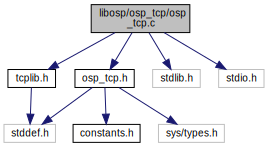
\includegraphics[width=341pt]{osp__tcp_8c__incl}
\end{center}
\end{figure}
\subsection*{Data Structures}
\begin{DoxyCompactItemize}
\item 
struct \mbox{\hyperlink{structosp__tcp__t}{osp\+\_\+tcp\+\_\+t}}
\begin{DoxyCompactList}\small\item\em Data structure containing O\+SP T\+CP layer internal variables. \end{DoxyCompactList}\end{DoxyCompactItemize}
\subsection*{Functions}
\begin{DoxyCompactItemize}
\item 
\mbox{\hyperlink{osp__tcp_8h_ac73f074c55d4549265c975cc8cffd349}{Osp\+\_\+tcp}} \mbox{\hyperlink{osp__tcp_8c_ae6c126a45386214aac909bc2b819a6d3}{osp\+\_\+tcp\+\_\+init}} (int port)
\begin{DoxyCompactList}\small\item\em Initialization function for the O\+SP T\+CP layer. \end{DoxyCompactList}\item 
int \mbox{\hyperlink{osp__tcp_8c_ab649aa1c24117770ecca7de43f94a3e8}{osp\+\_\+tcp\+\_\+connect}} (\mbox{\hyperlink{osp__tcp_8h_ac73f074c55d4549265c975cc8cffd349}{Osp\+\_\+tcp}} osp\+\_\+tcp)
\begin{DoxyCompactList}\small\item\em Blocking call that sets up server socket and waits for client connection In order to start a socket for a client (Android tablet, for instance), this must be called. It will block until a client establishes a connection, at which point it will return 0. \end{DoxyCompactList}\item 
char \mbox{\hyperlink{osp__tcp_8c_a5f810fc80c3683cdc05b5c4a3a785aa4}{osp\+\_\+tcp\+\_\+read\+\_\+req}} (\mbox{\hyperlink{osp__tcp_8h_ac73f074c55d4549265c975cc8cffd349}{Osp\+\_\+tcp}} osp\+\_\+tcp)
\begin{DoxyCompactList}\small\item\em Blocking call that returns the request sent by the connected client. The client can make a number of requests including updating the values running in the O\+SP real-\/time code (knee points, attack, release, gains, etc). The client can also request the number of underruns that have been counted from the audio driver, the number of bands that have been initially set up, etc. \end{DoxyCompactList}\item 
ssize\+\_\+t \mbox{\hyperlink{osp__tcp_8c_aa4b8a5a6a4fa9249a163f47c206f7e8d}{osp\+\_\+tcp\+\_\+read\+\_\+values}} (\mbox{\hyperlink{osp__tcp_8h_ac73f074c55d4549265c975cc8cffd349}{Osp\+\_\+tcp}} osp\+\_\+tcp, \mbox{\hyperlink{constants_8h_a2d1d78531fe12807c3852488556d5a4b}{osp\+\_\+user\+\_\+data}} $\ast$data, unsigned int size)
\begin{DoxyCompactList}\small\item\em Reads data from the T\+CP stream into the osp\+\_\+user\+\_\+data structure. \end{DoxyCompactList}\item 
ssize\+\_\+t \mbox{\hyperlink{osp__tcp_8c_aa2fe974658327f3586a54e6c2d57740b}{osp\+\_\+tcp\+\_\+read\+\_\+user\+\_\+packet}} (\mbox{\hyperlink{osp__tcp_8h_ac73f074c55d4549265c975cc8cffd349}{Osp\+\_\+tcp}} osp\+\_\+tcp, char $\ast$message, unsigned int size)
\item 
int \mbox{\hyperlink{osp__tcp_8c_af443391eb190ffb7bb8b13c19d5bbe67}{osp\+\_\+tcp\+\_\+send\+\_\+underruns}} (\mbox{\hyperlink{osp__tcp_8h_ac73f074c55d4549265c975cc8cffd349}{Osp\+\_\+tcp}} osp\+\_\+tcp, unsigned int underruns)
\begin{DoxyCompactList}\small\item\em Sends the number of underruns to client. \end{DoxyCompactList}\item 
int \mbox{\hyperlink{osp__tcp_8c_aab96e1d96e5f30b40bfed4b88cda820c}{osp\+\_\+tcp\+\_\+send\+\_\+num\+\_\+bands}} (\mbox{\hyperlink{osp__tcp_8h_ac73f074c55d4549265c975cc8cffd349}{Osp\+\_\+tcp}} osp\+\_\+tcp, unsigned char bands)
\begin{DoxyCompactList}\small\item\em Sends the number of bands to client. \end{DoxyCompactList}\item 
void \mbox{\hyperlink{osp__tcp_8c_ab998766bad97b04e79d93b25c2d54c14}{osp\+\_\+tcp\+\_\+close}} (\mbox{\hyperlink{osp__tcp_8h_ac73f074c55d4549265c975cc8cffd349}{Osp\+\_\+tcp}} osp\+\_\+tcp)
\begin{DoxyCompactList}\small\item\em Closes the T\+CP stream and frees the Osp\+\_\+tcp instance. \end{DoxyCompactList}\end{DoxyCompactItemize}


\subsection{Function Documentation}
\mbox{\Hypertarget{osp__tcp_8c_ab998766bad97b04e79d93b25c2d54c14}\label{osp__tcp_8c_ab998766bad97b04e79d93b25c2d54c14}} 
\index{osp\+\_\+tcp.\+c@{osp\+\_\+tcp.\+c}!osp\+\_\+tcp\+\_\+close@{osp\+\_\+tcp\+\_\+close}}
\index{osp\+\_\+tcp\+\_\+close@{osp\+\_\+tcp\+\_\+close}!osp\+\_\+tcp.\+c@{osp\+\_\+tcp.\+c}}
\subsubsection{\texorpdfstring{osp\+\_\+tcp\+\_\+close()}{osp\_tcp\_close()}}
{\footnotesize\ttfamily void osp\+\_\+tcp\+\_\+close (\begin{DoxyParamCaption}\item[{\mbox{\hyperlink{osp__tcp_8h_ac73f074c55d4549265c975cc8cffd349}{Osp\+\_\+tcp}}}]{osp\+\_\+tcp }\end{DoxyParamCaption})}



Closes the T\+CP stream and frees the Osp\+\_\+tcp instance. 

\begin{DoxySeeAlso}{See also}
\mbox{\hyperlink{structosp__tcp__t}{osp\+\_\+tcp\+\_\+t}} 
\end{DoxySeeAlso}

\begin{DoxyParams}{Parameters}
{\em osp\+\_\+tcp} & The instance of the Osp\+\_\+tcp variable that was returned from osp\+\_\+tcp\+\_\+init \\
\hline
\end{DoxyParams}
\mbox{\Hypertarget{osp__tcp_8c_ab649aa1c24117770ecca7de43f94a3e8}\label{osp__tcp_8c_ab649aa1c24117770ecca7de43f94a3e8}} 
\index{osp\+\_\+tcp.\+c@{osp\+\_\+tcp.\+c}!osp\+\_\+tcp\+\_\+connect@{osp\+\_\+tcp\+\_\+connect}}
\index{osp\+\_\+tcp\+\_\+connect@{osp\+\_\+tcp\+\_\+connect}!osp\+\_\+tcp.\+c@{osp\+\_\+tcp.\+c}}
\subsubsection{\texorpdfstring{osp\+\_\+tcp\+\_\+connect()}{osp\_tcp\_connect()}}
{\footnotesize\ttfamily int osp\+\_\+tcp\+\_\+connect (\begin{DoxyParamCaption}\item[{\mbox{\hyperlink{osp__tcp_8h_ac73f074c55d4549265c975cc8cffd349}{Osp\+\_\+tcp}}}]{osp\+\_\+tcp }\end{DoxyParamCaption})}



Blocking call that sets up server socket and waits for client connection In order to start a socket for a client (Android tablet, for instance), this must be called. It will block until a client establishes a connection, at which point it will return 0. 

\begin{DoxySeeAlso}{See also}
\mbox{\hyperlink{structosp__tcp__t}{osp\+\_\+tcp\+\_\+t}} 
\end{DoxySeeAlso}

\begin{DoxyParams}{Parameters}
{\em osp\+\_\+tcp} & The instance of the Osp\+\_\+tcp variable that was returned from osp\+\_\+tcp\+\_\+init \\
\hline
\end{DoxyParams}
\begin{DoxyReturn}{Returns}
Returns 0 on success, or -\/1 if there\textquotesingle{}s an error setting up the socket 
\end{DoxyReturn}
\mbox{\Hypertarget{osp__tcp_8c_ae6c126a45386214aac909bc2b819a6d3}\label{osp__tcp_8c_ae6c126a45386214aac909bc2b819a6d3}} 
\index{osp\+\_\+tcp.\+c@{osp\+\_\+tcp.\+c}!osp\+\_\+tcp\+\_\+init@{osp\+\_\+tcp\+\_\+init}}
\index{osp\+\_\+tcp\+\_\+init@{osp\+\_\+tcp\+\_\+init}!osp\+\_\+tcp.\+c@{osp\+\_\+tcp.\+c}}
\subsubsection{\texorpdfstring{osp\+\_\+tcp\+\_\+init()}{osp\_tcp\_init()}}
{\footnotesize\ttfamily \mbox{\hyperlink{osp__tcp_8h_ac73f074c55d4549265c975cc8cffd349}{Osp\+\_\+tcp}} osp\+\_\+tcp\+\_\+init (\begin{DoxyParamCaption}\item[{int}]{port }\end{DoxyParamCaption})}



Initialization function for the O\+SP T\+CP layer. 

\begin{DoxySeeAlso}{See also}
\mbox{\hyperlink{structosp__tcp__t}{osp\+\_\+tcp\+\_\+t}} 
\end{DoxySeeAlso}

\begin{DoxyParams}{Parameters}
{\em port} & The port in which to listen on for a client connection \\
\hline
\end{DoxyParams}
\begin{DoxyReturn}{Returns}
Returns the allocated instance of the O\+SP T\+CP layer data structure (\char`\"{}object\char`\"{}) 
\end{DoxyReturn}
\mbox{\Hypertarget{osp__tcp_8c_a5f810fc80c3683cdc05b5c4a3a785aa4}\label{osp__tcp_8c_a5f810fc80c3683cdc05b5c4a3a785aa4}} 
\index{osp\+\_\+tcp.\+c@{osp\+\_\+tcp.\+c}!osp\+\_\+tcp\+\_\+read\+\_\+req@{osp\+\_\+tcp\+\_\+read\+\_\+req}}
\index{osp\+\_\+tcp\+\_\+read\+\_\+req@{osp\+\_\+tcp\+\_\+read\+\_\+req}!osp\+\_\+tcp.\+c@{osp\+\_\+tcp.\+c}}
\subsubsection{\texorpdfstring{osp\+\_\+tcp\+\_\+read\+\_\+req()}{osp\_tcp\_read\_req()}}
{\footnotesize\ttfamily char osp\+\_\+tcp\+\_\+read\+\_\+req (\begin{DoxyParamCaption}\item[{\mbox{\hyperlink{osp__tcp_8h_ac73f074c55d4549265c975cc8cffd349}{Osp\+\_\+tcp}}}]{osp\+\_\+tcp }\end{DoxyParamCaption})}



Blocking call that returns the request sent by the connected client. The client can make a number of requests including updating the values running in the O\+SP real-\/time code (knee points, attack, release, gains, etc). The client can also request the number of underruns that have been counted from the audio driver, the number of bands that have been initially set up, etc. 

\begin{DoxySeeAlso}{See also}
\mbox{\hyperlink{structosp__tcp__t}{osp\+\_\+tcp\+\_\+t}} 

e\+\_\+osp\+\_\+tcp\+\_\+req\+\_\+t 
\end{DoxySeeAlso}

\begin{DoxyParams}{Parameters}
{\em osp\+\_\+tcp} & The instance of the Osp\+\_\+tcp variable that was returned from osp\+\_\+tcp\+\_\+init \\
\hline
\end{DoxyParams}
\begin{DoxyReturn}{Returns}
Returns the request sent by the client 
\end{DoxyReturn}
\mbox{\Hypertarget{osp__tcp_8c_aa2fe974658327f3586a54e6c2d57740b}\label{osp__tcp_8c_aa2fe974658327f3586a54e6c2d57740b}} 
\index{osp\+\_\+tcp.\+c@{osp\+\_\+tcp.\+c}!osp\+\_\+tcp\+\_\+read\+\_\+user\+\_\+packet@{osp\+\_\+tcp\+\_\+read\+\_\+user\+\_\+packet}}
\index{osp\+\_\+tcp\+\_\+read\+\_\+user\+\_\+packet@{osp\+\_\+tcp\+\_\+read\+\_\+user\+\_\+packet}!osp\+\_\+tcp.\+c@{osp\+\_\+tcp.\+c}}
\subsubsection{\texorpdfstring{osp\+\_\+tcp\+\_\+read\+\_\+user\+\_\+packet()}{osp\_tcp\_read\_user\_packet()}}
{\footnotesize\ttfamily ssize\+\_\+t osp\+\_\+tcp\+\_\+read\+\_\+user\+\_\+packet (\begin{DoxyParamCaption}\item[{\mbox{\hyperlink{osp__tcp_8h_ac73f074c55d4549265c975cc8cffd349}{Osp\+\_\+tcp}}}]{osp\+\_\+tcp,  }\item[{char $\ast$}]{message,  }\item[{unsigned int}]{size }\end{DoxyParamCaption})}

\mbox{\Hypertarget{osp__tcp_8c_aa4b8a5a6a4fa9249a163f47c206f7e8d}\label{osp__tcp_8c_aa4b8a5a6a4fa9249a163f47c206f7e8d}} 
\index{osp\+\_\+tcp.\+c@{osp\+\_\+tcp.\+c}!osp\+\_\+tcp\+\_\+read\+\_\+values@{osp\+\_\+tcp\+\_\+read\+\_\+values}}
\index{osp\+\_\+tcp\+\_\+read\+\_\+values@{osp\+\_\+tcp\+\_\+read\+\_\+values}!osp\+\_\+tcp.\+c@{osp\+\_\+tcp.\+c}}
\subsubsection{\texorpdfstring{osp\+\_\+tcp\+\_\+read\+\_\+values()}{osp\_tcp\_read\_values()}}
{\footnotesize\ttfamily ssize\+\_\+t osp\+\_\+tcp\+\_\+read\+\_\+values (\begin{DoxyParamCaption}\item[{\mbox{\hyperlink{osp__tcp_8h_ac73f074c55d4549265c975cc8cffd349}{Osp\+\_\+tcp}}}]{osp\+\_\+tcp,  }\item[{\mbox{\hyperlink{constants_8h_a2d1d78531fe12807c3852488556d5a4b}{osp\+\_\+user\+\_\+data}} $\ast$}]{data,  }\item[{unsigned int}]{size }\end{DoxyParamCaption})}



Reads data from the T\+CP stream into the osp\+\_\+user\+\_\+data structure. 

\begin{DoxySeeAlso}{See also}
\mbox{\hyperlink{constants_8h_a2d1d78531fe12807c3852488556d5a4b}{osp\+\_\+user\+\_\+data}} 

\mbox{\hyperlink{structosp__tcp__t}{osp\+\_\+tcp\+\_\+t}} 
\end{DoxySeeAlso}

\begin{DoxyParams}{Parameters}
{\em osp\+\_\+tcp} & The instance of the Osp\+\_\+tcp variable that was returned from osp\+\_\+tcp\+\_\+init \\
\hline
{\em data} & The osp\+\_\+user\+\_\+data structure that will be filled with data from the stream \\
\hline
{\em size} & The size of the data, in bytes, that are to be read from the stream since we\textquotesingle{}re reading into a struct of known size, passing a size variable might be redundant \\
\hline
\end{DoxyParams}
\begin{DoxyReturn}{Returns}
Returns 0 if the stream is no longer present (disconnect from client side, not error), -\/1 if there is an error reading from the server stream. Otherwise, the number of bytes read from the stream is returned 
\end{DoxyReturn}
\mbox{\Hypertarget{osp__tcp_8c_aab96e1d96e5f30b40bfed4b88cda820c}\label{osp__tcp_8c_aab96e1d96e5f30b40bfed4b88cda820c}} 
\index{osp\+\_\+tcp.\+c@{osp\+\_\+tcp.\+c}!osp\+\_\+tcp\+\_\+send\+\_\+num\+\_\+bands@{osp\+\_\+tcp\+\_\+send\+\_\+num\+\_\+bands}}
\index{osp\+\_\+tcp\+\_\+send\+\_\+num\+\_\+bands@{osp\+\_\+tcp\+\_\+send\+\_\+num\+\_\+bands}!osp\+\_\+tcp.\+c@{osp\+\_\+tcp.\+c}}
\subsubsection{\texorpdfstring{osp\+\_\+tcp\+\_\+send\+\_\+num\+\_\+bands()}{osp\_tcp\_send\_num\_bands()}}
{\footnotesize\ttfamily int osp\+\_\+tcp\+\_\+send\+\_\+num\+\_\+bands (\begin{DoxyParamCaption}\item[{\mbox{\hyperlink{osp__tcp_8h_ac73f074c55d4549265c975cc8cffd349}{Osp\+\_\+tcp}}}]{osp\+\_\+tcp,  }\item[{unsigned char}]{bands }\end{DoxyParamCaption})}



Sends the number of bands to client. 

\begin{DoxySeeAlso}{See also}
\mbox{\hyperlink{structosp__tcp__t}{osp\+\_\+tcp\+\_\+t}} 
\end{DoxySeeAlso}

\begin{DoxyParams}{Parameters}
{\em osp\+\_\+tcp} & The instance of the Osp\+\_\+tcp variable that was returned from osp\+\_\+tcp\+\_\+init \\
\hline
{\em bands} & Number of bands to report \\
\hline
\end{DoxyParams}
\begin{DoxyReturn}{Returns}
Returns 0 if success, -\/1 if there was an error writing to the stream 
\end{DoxyReturn}
\mbox{\Hypertarget{osp__tcp_8c_af443391eb190ffb7bb8b13c19d5bbe67}\label{osp__tcp_8c_af443391eb190ffb7bb8b13c19d5bbe67}} 
\index{osp\+\_\+tcp.\+c@{osp\+\_\+tcp.\+c}!osp\+\_\+tcp\+\_\+send\+\_\+underruns@{osp\+\_\+tcp\+\_\+send\+\_\+underruns}}
\index{osp\+\_\+tcp\+\_\+send\+\_\+underruns@{osp\+\_\+tcp\+\_\+send\+\_\+underruns}!osp\+\_\+tcp.\+c@{osp\+\_\+tcp.\+c}}
\subsubsection{\texorpdfstring{osp\+\_\+tcp\+\_\+send\+\_\+underruns()}{osp\_tcp\_send\_underruns()}}
{\footnotesize\ttfamily int osp\+\_\+tcp\+\_\+send\+\_\+underruns (\begin{DoxyParamCaption}\item[{\mbox{\hyperlink{osp__tcp_8h_ac73f074c55d4549265c975cc8cffd349}{Osp\+\_\+tcp}}}]{osp\+\_\+tcp,  }\item[{unsigned int}]{underruns }\end{DoxyParamCaption})}



Sends the number of underruns to client. 

\begin{DoxySeeAlso}{See also}
\mbox{\hyperlink{structosp__tcp__t}{osp\+\_\+tcp\+\_\+t}} 
\end{DoxySeeAlso}

\begin{DoxyParams}{Parameters}
{\em osp\+\_\+tcp} & The instance of the Osp\+\_\+tcp variable that was returned from osp\+\_\+tcp\+\_\+init \\
\hline
{\em underruns} & Number of underruns to report \\
\hline
\end{DoxyParams}
\begin{DoxyReturn}{Returns}
Returns 0 if success, -\/1 if there was an error writing to the stream 
\end{DoxyReturn}

\hypertarget{osp__tcp_8h}{}\section{libosp/osp\+\_\+tcp/osp\+\_\+tcp.h File Reference}
\label{osp__tcp_8h}\index{libosp/osp\+\_\+tcp/osp\+\_\+tcp.\+h@{libosp/osp\+\_\+tcp/osp\+\_\+tcp.\+h}}
{\ttfamily \#include $<$stddef.\+h$>$}\newline
{\ttfamily \#include \char`\"{}constants.\+h\char`\"{}}\newline
{\ttfamily \#include $<$sys/types.\+h$>$}\newline
{\ttfamily \#include $<$stdio.\+h$>$}\newline
{\ttfamily \#include $<$stdlib.\+h$>$}\newline
{\ttfamily \#include $<$string.\+h$>$}\newline
{\ttfamily \#include \char`\"{}jsmn.\+h\char`\"{}}\newline
Include dependency graph for osp\+\_\+tcp.\+h\+:
\nopagebreak
\begin{figure}[H]
\begin{center}
\leavevmode
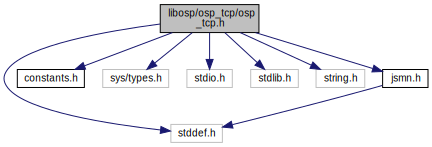
\includegraphics[width=350pt]{osp__tcp_8h__incl}
\end{center}
\end{figure}
This graph shows which files directly or indirectly include this file\+:
\nopagebreak
\begin{figure}[H]
\begin{center}
\leavevmode
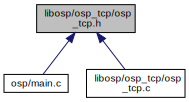
\includegraphics[width=262pt]{osp__tcp_8h__dep__incl}
\end{center}
\end{figure}
\subsection*{Macros}
\begin{DoxyCompactItemize}
\item 
\#define \mbox{\hyperlink{osp__tcp_8h_ad70c5cf43d6187190e18013388120a13}{O\+S\+P\+\_\+\+W\+R\+O\+N\+G\+\_\+\+V\+E\+R\+S\+I\+ON}}~0
\item 
\#define \mbox{\hyperlink{osp__tcp_8h_a88fd5366fe38af2b4219821affa068af}{O\+S\+P\+\_\+\+R\+E\+Q\+\_\+\+U\+P\+D\+A\+T\+E\+\_\+\+V\+A\+L\+U\+ES}}~1
\begin{DoxyCompactList}\small\item\em Request to set the values in the real-\/time O\+SP C application. \end{DoxyCompactList}\item 
\#define \mbox{\hyperlink{osp__tcp_8h_ac11866b2a978a05955e5e89a0b1107d1}{O\+S\+P\+\_\+\+R\+E\+Q\+\_\+\+G\+E\+T\+\_\+\+U\+N\+D\+E\+R\+R\+U\+NS}}~2
\begin{DoxyCompactList}\small\item\em Request to get number of underruns from real-\/time O\+SP application. \end{DoxyCompactList}\item 
\#define \mbox{\hyperlink{osp__tcp_8h_a491961372a3e01bdc57287e4c2b94d47}{O\+S\+P\+\_\+\+R\+E\+Q\+\_\+\+U\+S\+E\+R\+\_\+\+ID}}~3
\item 
\#define \mbox{\hyperlink{osp__tcp_8h_ae9f1e494220fc2ed6c557185f2630e09}{O\+S\+P\+\_\+\+R\+E\+Q\+\_\+\+U\+S\+E\+R\+\_\+\+A\+C\+T\+I\+ON}}~4
\item 
\#define \mbox{\hyperlink{osp__tcp_8h_a2ff6a0a7b702e21aaa12904ebe0b983a}{O\+S\+P\+\_\+\+R\+E\+Q\+\_\+\+G\+E\+T\+\_\+\+N\+U\+M\+\_\+\+B\+A\+N\+DS}}~5
\item 
\#define \mbox{\hyperlink{osp__tcp_8h_aea93a99440c7bb1ee573213b6df715c0}{O\+S\+P\+\_\+\+D\+I\+S\+C\+O\+N\+N\+E\+CT}}~6
\item 
\#define \mbox{\hyperlink{osp__tcp_8h_afe108e38ff4f06dfe9ea602ab9f23ab0}{O\+S\+P\+\_\+\+R\+E\+Q\+\_\+\+L\+A\+ST}}~7
\begin{DoxyCompactList}\small\item\em This exists so we can test if an inc packet is one we recognize. \end{DoxyCompactList}\item 
\#define \mbox{\hyperlink{osp__tcp_8h_aeca6c1645aad424bb1e7b14ae09829b3}{R\+E\+A\+D\+\_\+\+R\+E\+Q\+U\+E\+S\+T\+\_\+\+L\+E\+N\+\_\+\+J\+S\+ON}}~36
\item 
\#define \mbox{\hyperlink{osp__tcp_8h_a094486f28d8cd6fca095dbbdaf670b7e}{U\+S\+E\+R\+\_\+\+L\+E\+N\+\_\+\+J\+S\+ON}}~8
\item 
\#define \mbox{\hyperlink{osp__tcp_8h_acbb575a53449acaade075615da61307d}{U\+S\+E\+R\+\_\+\+J\+S\+ON}}~10
\item 
\#define \mbox{\hyperlink{osp__tcp_8h_ade9a9413664417f0fa4d89a11f9cbaed}{H\+A\+\_\+\+S\+T\+A\+T\+E\+\_\+\+J\+S\+ON}}~257
\end{DoxyCompactItemize}
\subsection*{Typedefs}
\begin{DoxyCompactItemize}
\item 
typedef struct \mbox{\hyperlink{structosp__tcp__t}{osp\+\_\+tcp\+\_\+t}} $\ast$ \mbox{\hyperlink{osp__tcp_8h_ac73f074c55d4549265c975cc8cffd349}{Osp\+\_\+tcp}}
\end{DoxyCompactItemize}
\subsection*{Functions}
\begin{DoxyCompactItemize}
\item 
\mbox{\hyperlink{osp__tcp_8h_ac73f074c55d4549265c975cc8cffd349}{Osp\+\_\+tcp}} \mbox{\hyperlink{osp__tcp_8h_ae6c126a45386214aac909bc2b819a6d3}{osp\+\_\+tcp\+\_\+init}} (int port)
\begin{DoxyCompactList}\small\item\em Initialization function for the O\+SP T\+CP layer. \end{DoxyCompactList}\item 
int \mbox{\hyperlink{osp__tcp_8h_ab649aa1c24117770ecca7de43f94a3e8}{osp\+\_\+tcp\+\_\+connect}} (\mbox{\hyperlink{osp__tcp_8h_ac73f074c55d4549265c975cc8cffd349}{Osp\+\_\+tcp}} osp\+\_\+tcp)
\begin{DoxyCompactList}\small\item\em Blocking call that sets up server socket and waits for client connection In order to start a socket for a client (Android tablet, for instance), this must be called. It will block until a client establishes a connection, at which point it will return 0. \end{DoxyCompactList}\item 
int \mbox{\hyperlink{osp__tcp_8h_a55d011dc599c183aa80780931d5fafe0}{osp\+\_\+tcp\+\_\+read\+\_\+req}} (\mbox{\hyperlink{osp__tcp_8h_ac73f074c55d4549265c975cc8cffd349}{Osp\+\_\+tcp}} osp\+\_\+tcp)
\begin{DoxyCompactList}\small\item\em Blocking call that returns the request sent by the connected client. The client can make a number of requests including updating the values running in the O\+SP real-\/time code (knee points, attack, release, gains, etc). The client can also request the number of underruns that have been counted from the audio driver, the number of bands that have been initially set up, etc. \end{DoxyCompactList}\item 
ssize\+\_\+t \mbox{\hyperlink{osp__tcp_8h_a31da083ff61e714c57e6ac37100e8e15}{osp\+\_\+4afc\+\_\+read\+\_\+values}} (\mbox{\hyperlink{osp__tcp_8h_ac73f074c55d4549265c975cc8cffd349}{Osp\+\_\+tcp}} osp\+\_\+tcp, char $\ast$file\+\_\+path, unsigned int size)
\item 
ssize\+\_\+t \mbox{\hyperlink{osp__tcp_8h_aa4b8a5a6a4fa9249a163f47c206f7e8d}{osp\+\_\+tcp\+\_\+read\+\_\+values}} (\mbox{\hyperlink{osp__tcp_8h_ac73f074c55d4549265c975cc8cffd349}{Osp\+\_\+tcp}} osp\+\_\+tcp, \mbox{\hyperlink{constants_8h_a2d1d78531fe12807c3852488556d5a4b}{osp\+\_\+user\+\_\+data}} $\ast$data, unsigned int size)
\begin{DoxyCompactList}\small\item\em Reads data from the T\+CP stream into the osp\+\_\+user\+\_\+data structure. \end{DoxyCompactList}\item 
int \mbox{\hyperlink{osp__tcp_8h_af443391eb190ffb7bb8b13c19d5bbe67}{osp\+\_\+tcp\+\_\+send\+\_\+underruns}} (\mbox{\hyperlink{osp__tcp_8h_ac73f074c55d4549265c975cc8cffd349}{Osp\+\_\+tcp}} osp\+\_\+tcp, unsigned int underruns)
\begin{DoxyCompactList}\small\item\em Sends the number of underruns to client. \end{DoxyCompactList}\item 
ssize\+\_\+t \mbox{\hyperlink{osp__tcp_8h_aa2fe974658327f3586a54e6c2d57740b}{osp\+\_\+tcp\+\_\+read\+\_\+user\+\_\+packet}} (\mbox{\hyperlink{osp__tcp_8h_ac73f074c55d4549265c975cc8cffd349}{Osp\+\_\+tcp}} osp\+\_\+tcp, char $\ast$message, unsigned int size)
\item 
int \mbox{\hyperlink{osp__tcp_8h_aab96e1d96e5f30b40bfed4b88cda820c}{osp\+\_\+tcp\+\_\+send\+\_\+num\+\_\+bands}} (\mbox{\hyperlink{osp__tcp_8h_ac73f074c55d4549265c975cc8cffd349}{Osp\+\_\+tcp}} osp\+\_\+tcp, unsigned char bands)
\begin{DoxyCompactList}\small\item\em Sends the number of bands to client. \end{DoxyCompactList}\item 
void \mbox{\hyperlink{osp__tcp_8h_ab998766bad97b04e79d93b25c2d54c14}{osp\+\_\+tcp\+\_\+close}} (\mbox{\hyperlink{osp__tcp_8h_ac73f074c55d4549265c975cc8cffd349}{Osp\+\_\+tcp}} osp\+\_\+tcp)
\begin{DoxyCompactList}\small\item\em Closes the T\+CP stream and frees the Osp\+\_\+tcp instance. \end{DoxyCompactList}\end{DoxyCompactItemize}


\subsection{Detailed Description}
This layer is the interface to the client side of the O\+SP application. 

\subsection{Macro Definition Documentation}
\mbox{\Hypertarget{osp__tcp_8h_ade9a9413664417f0fa4d89a11f9cbaed}\label{osp__tcp_8h_ade9a9413664417f0fa4d89a11f9cbaed}} 
\index{osp\+\_\+tcp.\+h@{osp\+\_\+tcp.\+h}!H\+A\+\_\+\+S\+T\+A\+T\+E\+\_\+\+J\+S\+ON@{H\+A\+\_\+\+S\+T\+A\+T\+E\+\_\+\+J\+S\+ON}}
\index{H\+A\+\_\+\+S\+T\+A\+T\+E\+\_\+\+J\+S\+ON@{H\+A\+\_\+\+S\+T\+A\+T\+E\+\_\+\+J\+S\+ON}!osp\+\_\+tcp.\+h@{osp\+\_\+tcp.\+h}}
\subsubsection{\texorpdfstring{H\+A\+\_\+\+S\+T\+A\+T\+E\+\_\+\+J\+S\+ON}{HA\_STATE\_JSON}}
{\footnotesize\ttfamily \#define H\+A\+\_\+\+S\+T\+A\+T\+E\+\_\+\+J\+S\+ON~257}

\mbox{\Hypertarget{osp__tcp_8h_aea93a99440c7bb1ee573213b6df715c0}\label{osp__tcp_8h_aea93a99440c7bb1ee573213b6df715c0}} 
\index{osp\+\_\+tcp.\+h@{osp\+\_\+tcp.\+h}!O\+S\+P\+\_\+\+D\+I\+S\+C\+O\+N\+N\+E\+CT@{O\+S\+P\+\_\+\+D\+I\+S\+C\+O\+N\+N\+E\+CT}}
\index{O\+S\+P\+\_\+\+D\+I\+S\+C\+O\+N\+N\+E\+CT@{O\+S\+P\+\_\+\+D\+I\+S\+C\+O\+N\+N\+E\+CT}!osp\+\_\+tcp.\+h@{osp\+\_\+tcp.\+h}}
\subsubsection{\texorpdfstring{O\+S\+P\+\_\+\+D\+I\+S\+C\+O\+N\+N\+E\+CT}{OSP\_DISCONNECT}}
{\footnotesize\ttfamily \#define O\+S\+P\+\_\+\+D\+I\+S\+C\+O\+N\+N\+E\+CT~6}

\mbox{\Hypertarget{osp__tcp_8h_a2ff6a0a7b702e21aaa12904ebe0b983a}\label{osp__tcp_8h_a2ff6a0a7b702e21aaa12904ebe0b983a}} 
\index{osp\+\_\+tcp.\+h@{osp\+\_\+tcp.\+h}!O\+S\+P\+\_\+\+R\+E\+Q\+\_\+\+G\+E\+T\+\_\+\+N\+U\+M\+\_\+\+B\+A\+N\+DS@{O\+S\+P\+\_\+\+R\+E\+Q\+\_\+\+G\+E\+T\+\_\+\+N\+U\+M\+\_\+\+B\+A\+N\+DS}}
\index{O\+S\+P\+\_\+\+R\+E\+Q\+\_\+\+G\+E\+T\+\_\+\+N\+U\+M\+\_\+\+B\+A\+N\+DS@{O\+S\+P\+\_\+\+R\+E\+Q\+\_\+\+G\+E\+T\+\_\+\+N\+U\+M\+\_\+\+B\+A\+N\+DS}!osp\+\_\+tcp.\+h@{osp\+\_\+tcp.\+h}}
\subsubsection{\texorpdfstring{O\+S\+P\+\_\+\+R\+E\+Q\+\_\+\+G\+E\+T\+\_\+\+N\+U\+M\+\_\+\+B\+A\+N\+DS}{OSP\_REQ\_GET\_NUM\_BANDS}}
{\footnotesize\ttfamily \#define O\+S\+P\+\_\+\+R\+E\+Q\+\_\+\+G\+E\+T\+\_\+\+N\+U\+M\+\_\+\+B\+A\+N\+DS~5}

\mbox{\Hypertarget{osp__tcp_8h_ac11866b2a978a05955e5e89a0b1107d1}\label{osp__tcp_8h_ac11866b2a978a05955e5e89a0b1107d1}} 
\index{osp\+\_\+tcp.\+h@{osp\+\_\+tcp.\+h}!O\+S\+P\+\_\+\+R\+E\+Q\+\_\+\+G\+E\+T\+\_\+\+U\+N\+D\+E\+R\+R\+U\+NS@{O\+S\+P\+\_\+\+R\+E\+Q\+\_\+\+G\+E\+T\+\_\+\+U\+N\+D\+E\+R\+R\+U\+NS}}
\index{O\+S\+P\+\_\+\+R\+E\+Q\+\_\+\+G\+E\+T\+\_\+\+U\+N\+D\+E\+R\+R\+U\+NS@{O\+S\+P\+\_\+\+R\+E\+Q\+\_\+\+G\+E\+T\+\_\+\+U\+N\+D\+E\+R\+R\+U\+NS}!osp\+\_\+tcp.\+h@{osp\+\_\+tcp.\+h}}
\subsubsection{\texorpdfstring{O\+S\+P\+\_\+\+R\+E\+Q\+\_\+\+G\+E\+T\+\_\+\+U\+N\+D\+E\+R\+R\+U\+NS}{OSP\_REQ\_GET\_UNDERRUNS}}
{\footnotesize\ttfamily \#define O\+S\+P\+\_\+\+R\+E\+Q\+\_\+\+G\+E\+T\+\_\+\+U\+N\+D\+E\+R\+R\+U\+NS~2}



Request to get number of underruns from real-\/time O\+SP application. 

\mbox{\Hypertarget{osp__tcp_8h_afe108e38ff4f06dfe9ea602ab9f23ab0}\label{osp__tcp_8h_afe108e38ff4f06dfe9ea602ab9f23ab0}} 
\index{osp\+\_\+tcp.\+h@{osp\+\_\+tcp.\+h}!O\+S\+P\+\_\+\+R\+E\+Q\+\_\+\+L\+A\+ST@{O\+S\+P\+\_\+\+R\+E\+Q\+\_\+\+L\+A\+ST}}
\index{O\+S\+P\+\_\+\+R\+E\+Q\+\_\+\+L\+A\+ST@{O\+S\+P\+\_\+\+R\+E\+Q\+\_\+\+L\+A\+ST}!osp\+\_\+tcp.\+h@{osp\+\_\+tcp.\+h}}
\subsubsection{\texorpdfstring{O\+S\+P\+\_\+\+R\+E\+Q\+\_\+\+L\+A\+ST}{OSP\_REQ\_LAST}}
{\footnotesize\ttfamily \#define O\+S\+P\+\_\+\+R\+E\+Q\+\_\+\+L\+A\+ST~7}



This exists so we can test if an inc packet is one we recognize. 

\mbox{\Hypertarget{osp__tcp_8h_a88fd5366fe38af2b4219821affa068af}\label{osp__tcp_8h_a88fd5366fe38af2b4219821affa068af}} 
\index{osp\+\_\+tcp.\+h@{osp\+\_\+tcp.\+h}!O\+S\+P\+\_\+\+R\+E\+Q\+\_\+\+U\+P\+D\+A\+T\+E\+\_\+\+V\+A\+L\+U\+ES@{O\+S\+P\+\_\+\+R\+E\+Q\+\_\+\+U\+P\+D\+A\+T\+E\+\_\+\+V\+A\+L\+U\+ES}}
\index{O\+S\+P\+\_\+\+R\+E\+Q\+\_\+\+U\+P\+D\+A\+T\+E\+\_\+\+V\+A\+L\+U\+ES@{O\+S\+P\+\_\+\+R\+E\+Q\+\_\+\+U\+P\+D\+A\+T\+E\+\_\+\+V\+A\+L\+U\+ES}!osp\+\_\+tcp.\+h@{osp\+\_\+tcp.\+h}}
\subsubsection{\texorpdfstring{O\+S\+P\+\_\+\+R\+E\+Q\+\_\+\+U\+P\+D\+A\+T\+E\+\_\+\+V\+A\+L\+U\+ES}{OSP\_REQ\_UPDATE\_VALUES}}
{\footnotesize\ttfamily \#define O\+S\+P\+\_\+\+R\+E\+Q\+\_\+\+U\+P\+D\+A\+T\+E\+\_\+\+V\+A\+L\+U\+ES~1}



Request to set the values in the real-\/time O\+SP C application. 

\mbox{\Hypertarget{osp__tcp_8h_ae9f1e494220fc2ed6c557185f2630e09}\label{osp__tcp_8h_ae9f1e494220fc2ed6c557185f2630e09}} 
\index{osp\+\_\+tcp.\+h@{osp\+\_\+tcp.\+h}!O\+S\+P\+\_\+\+R\+E\+Q\+\_\+\+U\+S\+E\+R\+\_\+\+A\+C\+T\+I\+ON@{O\+S\+P\+\_\+\+R\+E\+Q\+\_\+\+U\+S\+E\+R\+\_\+\+A\+C\+T\+I\+ON}}
\index{O\+S\+P\+\_\+\+R\+E\+Q\+\_\+\+U\+S\+E\+R\+\_\+\+A\+C\+T\+I\+ON@{O\+S\+P\+\_\+\+R\+E\+Q\+\_\+\+U\+S\+E\+R\+\_\+\+A\+C\+T\+I\+ON}!osp\+\_\+tcp.\+h@{osp\+\_\+tcp.\+h}}
\subsubsection{\texorpdfstring{O\+S\+P\+\_\+\+R\+E\+Q\+\_\+\+U\+S\+E\+R\+\_\+\+A\+C\+T\+I\+ON}{OSP\_REQ\_USER\_ACTION}}
{\footnotesize\ttfamily \#define O\+S\+P\+\_\+\+R\+E\+Q\+\_\+\+U\+S\+E\+R\+\_\+\+A\+C\+T\+I\+ON~4}

\mbox{\Hypertarget{osp__tcp_8h_a491961372a3e01bdc57287e4c2b94d47}\label{osp__tcp_8h_a491961372a3e01bdc57287e4c2b94d47}} 
\index{osp\+\_\+tcp.\+h@{osp\+\_\+tcp.\+h}!O\+S\+P\+\_\+\+R\+E\+Q\+\_\+\+U\+S\+E\+R\+\_\+\+ID@{O\+S\+P\+\_\+\+R\+E\+Q\+\_\+\+U\+S\+E\+R\+\_\+\+ID}}
\index{O\+S\+P\+\_\+\+R\+E\+Q\+\_\+\+U\+S\+E\+R\+\_\+\+ID@{O\+S\+P\+\_\+\+R\+E\+Q\+\_\+\+U\+S\+E\+R\+\_\+\+ID}!osp\+\_\+tcp.\+h@{osp\+\_\+tcp.\+h}}
\subsubsection{\texorpdfstring{O\+S\+P\+\_\+\+R\+E\+Q\+\_\+\+U\+S\+E\+R\+\_\+\+ID}{OSP\_REQ\_USER\_ID}}
{\footnotesize\ttfamily \#define O\+S\+P\+\_\+\+R\+E\+Q\+\_\+\+U\+S\+E\+R\+\_\+\+ID~3}

\mbox{\Hypertarget{osp__tcp_8h_ad70c5cf43d6187190e18013388120a13}\label{osp__tcp_8h_ad70c5cf43d6187190e18013388120a13}} 
\index{osp\+\_\+tcp.\+h@{osp\+\_\+tcp.\+h}!O\+S\+P\+\_\+\+W\+R\+O\+N\+G\+\_\+\+V\+E\+R\+S\+I\+ON@{O\+S\+P\+\_\+\+W\+R\+O\+N\+G\+\_\+\+V\+E\+R\+S\+I\+ON}}
\index{O\+S\+P\+\_\+\+W\+R\+O\+N\+G\+\_\+\+V\+E\+R\+S\+I\+ON@{O\+S\+P\+\_\+\+W\+R\+O\+N\+G\+\_\+\+V\+E\+R\+S\+I\+ON}!osp\+\_\+tcp.\+h@{osp\+\_\+tcp.\+h}}
\subsubsection{\texorpdfstring{O\+S\+P\+\_\+\+W\+R\+O\+N\+G\+\_\+\+V\+E\+R\+S\+I\+ON}{OSP\_WRONG\_VERSION}}
{\footnotesize\ttfamily \#define O\+S\+P\+\_\+\+W\+R\+O\+N\+G\+\_\+\+V\+E\+R\+S\+I\+ON~0}

\mbox{\Hypertarget{osp__tcp_8h_aeca6c1645aad424bb1e7b14ae09829b3}\label{osp__tcp_8h_aeca6c1645aad424bb1e7b14ae09829b3}} 
\index{osp\+\_\+tcp.\+h@{osp\+\_\+tcp.\+h}!R\+E\+A\+D\+\_\+\+R\+E\+Q\+U\+E\+S\+T\+\_\+\+L\+E\+N\+\_\+\+J\+S\+ON@{R\+E\+A\+D\+\_\+\+R\+E\+Q\+U\+E\+S\+T\+\_\+\+L\+E\+N\+\_\+\+J\+S\+ON}}
\index{R\+E\+A\+D\+\_\+\+R\+E\+Q\+U\+E\+S\+T\+\_\+\+L\+E\+N\+\_\+\+J\+S\+ON@{R\+E\+A\+D\+\_\+\+R\+E\+Q\+U\+E\+S\+T\+\_\+\+L\+E\+N\+\_\+\+J\+S\+ON}!osp\+\_\+tcp.\+h@{osp\+\_\+tcp.\+h}}
\subsubsection{\texorpdfstring{R\+E\+A\+D\+\_\+\+R\+E\+Q\+U\+E\+S\+T\+\_\+\+L\+E\+N\+\_\+\+J\+S\+ON}{READ\_REQUEST\_LEN\_JSON}}
{\footnotesize\ttfamily \#define R\+E\+A\+D\+\_\+\+R\+E\+Q\+U\+E\+S\+T\+\_\+\+L\+E\+N\+\_\+\+J\+S\+ON~36}

\mbox{\Hypertarget{osp__tcp_8h_acbb575a53449acaade075615da61307d}\label{osp__tcp_8h_acbb575a53449acaade075615da61307d}} 
\index{osp\+\_\+tcp.\+h@{osp\+\_\+tcp.\+h}!U\+S\+E\+R\+\_\+\+J\+S\+ON@{U\+S\+E\+R\+\_\+\+J\+S\+ON}}
\index{U\+S\+E\+R\+\_\+\+J\+S\+ON@{U\+S\+E\+R\+\_\+\+J\+S\+ON}!osp\+\_\+tcp.\+h@{osp\+\_\+tcp.\+h}}
\subsubsection{\texorpdfstring{U\+S\+E\+R\+\_\+\+J\+S\+ON}{USER\_JSON}}
{\footnotesize\ttfamily \#define U\+S\+E\+R\+\_\+\+J\+S\+ON~10}

\mbox{\Hypertarget{osp__tcp_8h_a094486f28d8cd6fca095dbbdaf670b7e}\label{osp__tcp_8h_a094486f28d8cd6fca095dbbdaf670b7e}} 
\index{osp\+\_\+tcp.\+h@{osp\+\_\+tcp.\+h}!U\+S\+E\+R\+\_\+\+L\+E\+N\+\_\+\+J\+S\+ON@{U\+S\+E\+R\+\_\+\+L\+E\+N\+\_\+\+J\+S\+ON}}
\index{U\+S\+E\+R\+\_\+\+L\+E\+N\+\_\+\+J\+S\+ON@{U\+S\+E\+R\+\_\+\+L\+E\+N\+\_\+\+J\+S\+ON}!osp\+\_\+tcp.\+h@{osp\+\_\+tcp.\+h}}
\subsubsection{\texorpdfstring{U\+S\+E\+R\+\_\+\+L\+E\+N\+\_\+\+J\+S\+ON}{USER\_LEN\_JSON}}
{\footnotesize\ttfamily \#define U\+S\+E\+R\+\_\+\+L\+E\+N\+\_\+\+J\+S\+ON~8}



\subsection{Typedef Documentation}
\mbox{\Hypertarget{osp__tcp_8h_ac73f074c55d4549265c975cc8cffd349}\label{osp__tcp_8h_ac73f074c55d4549265c975cc8cffd349}} 
\index{osp\+\_\+tcp.\+h@{osp\+\_\+tcp.\+h}!Osp\+\_\+tcp@{Osp\+\_\+tcp}}
\index{Osp\+\_\+tcp@{Osp\+\_\+tcp}!osp\+\_\+tcp.\+h@{osp\+\_\+tcp.\+h}}
\subsubsection{\texorpdfstring{Osp\+\_\+tcp}{Osp\_tcp}}
{\footnotesize\ttfamily typedef struct \mbox{\hyperlink{structosp__tcp__t}{osp\+\_\+tcp\+\_\+t}}$\ast$ \mbox{\hyperlink{osp__tcp_8h_ac73f074c55d4549265c975cc8cffd349}{Osp\+\_\+tcp}}}



\subsection{Function Documentation}
\mbox{\Hypertarget{osp__tcp_8h_a31da083ff61e714c57e6ac37100e8e15}\label{osp__tcp_8h_a31da083ff61e714c57e6ac37100e8e15}} 
\index{osp\+\_\+tcp.\+h@{osp\+\_\+tcp.\+h}!osp\+\_\+4afc\+\_\+read\+\_\+values@{osp\+\_\+4afc\+\_\+read\+\_\+values}}
\index{osp\+\_\+4afc\+\_\+read\+\_\+values@{osp\+\_\+4afc\+\_\+read\+\_\+values}!osp\+\_\+tcp.\+h@{osp\+\_\+tcp.\+h}}
\subsubsection{\texorpdfstring{osp\+\_\+4afc\+\_\+read\+\_\+values()}{osp\_4afc\_read\_values()}}
{\footnotesize\ttfamily ssize\+\_\+t osp\+\_\+4afc\+\_\+read\+\_\+values (\begin{DoxyParamCaption}\item[{\mbox{\hyperlink{osp__tcp_8h_ac73f074c55d4549265c975cc8cffd349}{Osp\+\_\+tcp}}}]{osp\+\_\+tcp,  }\item[{char $\ast$}]{file\+\_\+path,  }\item[{unsigned int}]{size }\end{DoxyParamCaption})}

\mbox{\Hypertarget{osp__tcp_8h_ab998766bad97b04e79d93b25c2d54c14}\label{osp__tcp_8h_ab998766bad97b04e79d93b25c2d54c14}} 
\index{osp\+\_\+tcp.\+h@{osp\+\_\+tcp.\+h}!osp\+\_\+tcp\+\_\+close@{osp\+\_\+tcp\+\_\+close}}
\index{osp\+\_\+tcp\+\_\+close@{osp\+\_\+tcp\+\_\+close}!osp\+\_\+tcp.\+h@{osp\+\_\+tcp.\+h}}
\subsubsection{\texorpdfstring{osp\+\_\+tcp\+\_\+close()}{osp\_tcp\_close()}}
{\footnotesize\ttfamily void osp\+\_\+tcp\+\_\+close (\begin{DoxyParamCaption}\item[{\mbox{\hyperlink{osp__tcp_8h_ac73f074c55d4549265c975cc8cffd349}{Osp\+\_\+tcp}}}]{osp\+\_\+tcp }\end{DoxyParamCaption})}



Closes the T\+CP stream and frees the Osp\+\_\+tcp instance. 

\begin{DoxySeeAlso}{See also}
\mbox{\hyperlink{structosp__tcp__t}{osp\+\_\+tcp\+\_\+t}} 
\end{DoxySeeAlso}

\begin{DoxyParams}{Parameters}
{\em osp\+\_\+tcp} & The instance of the Osp\+\_\+tcp variable that was returned from osp\+\_\+tcp\+\_\+init \\
\hline
\end{DoxyParams}
\mbox{\Hypertarget{osp__tcp_8h_ab649aa1c24117770ecca7de43f94a3e8}\label{osp__tcp_8h_ab649aa1c24117770ecca7de43f94a3e8}} 
\index{osp\+\_\+tcp.\+h@{osp\+\_\+tcp.\+h}!osp\+\_\+tcp\+\_\+connect@{osp\+\_\+tcp\+\_\+connect}}
\index{osp\+\_\+tcp\+\_\+connect@{osp\+\_\+tcp\+\_\+connect}!osp\+\_\+tcp.\+h@{osp\+\_\+tcp.\+h}}
\subsubsection{\texorpdfstring{osp\+\_\+tcp\+\_\+connect()}{osp\_tcp\_connect()}}
{\footnotesize\ttfamily int osp\+\_\+tcp\+\_\+connect (\begin{DoxyParamCaption}\item[{\mbox{\hyperlink{osp__tcp_8h_ac73f074c55d4549265c975cc8cffd349}{Osp\+\_\+tcp}}}]{osp\+\_\+tcp }\end{DoxyParamCaption})}



Blocking call that sets up server socket and waits for client connection In order to start a socket for a client (Android tablet, for instance), this must be called. It will block until a client establishes a connection, at which point it will return 0. 

\begin{DoxySeeAlso}{See also}
\mbox{\hyperlink{structosp__tcp__t}{osp\+\_\+tcp\+\_\+t}} 
\end{DoxySeeAlso}

\begin{DoxyParams}{Parameters}
{\em osp\+\_\+tcp} & The instance of the Osp\+\_\+tcp variable that was returned from osp\+\_\+tcp\+\_\+init \\
\hline
\end{DoxyParams}
\begin{DoxyReturn}{Returns}
Returns 0 on success, or -\/1 if there\textquotesingle{}s an error setting up the socket 
\end{DoxyReturn}
\mbox{\Hypertarget{osp__tcp_8h_ae6c126a45386214aac909bc2b819a6d3}\label{osp__tcp_8h_ae6c126a45386214aac909bc2b819a6d3}} 
\index{osp\+\_\+tcp.\+h@{osp\+\_\+tcp.\+h}!osp\+\_\+tcp\+\_\+init@{osp\+\_\+tcp\+\_\+init}}
\index{osp\+\_\+tcp\+\_\+init@{osp\+\_\+tcp\+\_\+init}!osp\+\_\+tcp.\+h@{osp\+\_\+tcp.\+h}}
\subsubsection{\texorpdfstring{osp\+\_\+tcp\+\_\+init()}{osp\_tcp\_init()}}
{\footnotesize\ttfamily \mbox{\hyperlink{osp__tcp_8h_ac73f074c55d4549265c975cc8cffd349}{Osp\+\_\+tcp}} osp\+\_\+tcp\+\_\+init (\begin{DoxyParamCaption}\item[{int}]{port }\end{DoxyParamCaption})}



Initialization function for the O\+SP T\+CP layer. 

\begin{DoxySeeAlso}{See also}
\mbox{\hyperlink{structosp__tcp__t}{osp\+\_\+tcp\+\_\+t}} 
\end{DoxySeeAlso}

\begin{DoxyParams}{Parameters}
{\em port} & The port in which to listen on for a client connection \\
\hline
\end{DoxyParams}
\begin{DoxyReturn}{Returns}
Returns the allocated instance of the O\+SP T\+CP layer data structure (\char`\"{}object\char`\"{}) 
\end{DoxyReturn}
\mbox{\Hypertarget{osp__tcp_8h_a55d011dc599c183aa80780931d5fafe0}\label{osp__tcp_8h_a55d011dc599c183aa80780931d5fafe0}} 
\index{osp\+\_\+tcp.\+h@{osp\+\_\+tcp.\+h}!osp\+\_\+tcp\+\_\+read\+\_\+req@{osp\+\_\+tcp\+\_\+read\+\_\+req}}
\index{osp\+\_\+tcp\+\_\+read\+\_\+req@{osp\+\_\+tcp\+\_\+read\+\_\+req}!osp\+\_\+tcp.\+h@{osp\+\_\+tcp.\+h}}
\subsubsection{\texorpdfstring{osp\+\_\+tcp\+\_\+read\+\_\+req()}{osp\_tcp\_read\_req()}}
{\footnotesize\ttfamily int osp\+\_\+tcp\+\_\+read\+\_\+req (\begin{DoxyParamCaption}\item[{\mbox{\hyperlink{osp__tcp_8h_ac73f074c55d4549265c975cc8cffd349}{Osp\+\_\+tcp}}}]{osp\+\_\+tcp }\end{DoxyParamCaption})}



Blocking call that returns the request sent by the connected client. The client can make a number of requests including updating the values running in the O\+SP real-\/time code (knee points, attack, release, gains, etc). The client can also request the number of underruns that have been counted from the audio driver, the number of bands that have been initially set up, etc. 

\begin{DoxySeeAlso}{See also}
\mbox{\hyperlink{structosp__tcp__t}{osp\+\_\+tcp\+\_\+t}} 

e\+\_\+osp\+\_\+tcp\+\_\+req\+\_\+t 
\end{DoxySeeAlso}

\begin{DoxyParams}{Parameters}
{\em osp\+\_\+tcp} & The instance of the Osp\+\_\+tcp variable that was returned from osp\+\_\+tcp\+\_\+init \\
\hline
\end{DoxyParams}
\begin{DoxyReturn}{Returns}
Returns the request sent by the client 
\end{DoxyReturn}
\mbox{\Hypertarget{osp__tcp_8h_aa2fe974658327f3586a54e6c2d57740b}\label{osp__tcp_8h_aa2fe974658327f3586a54e6c2d57740b}} 
\index{osp\+\_\+tcp.\+h@{osp\+\_\+tcp.\+h}!osp\+\_\+tcp\+\_\+read\+\_\+user\+\_\+packet@{osp\+\_\+tcp\+\_\+read\+\_\+user\+\_\+packet}}
\index{osp\+\_\+tcp\+\_\+read\+\_\+user\+\_\+packet@{osp\+\_\+tcp\+\_\+read\+\_\+user\+\_\+packet}!osp\+\_\+tcp.\+h@{osp\+\_\+tcp.\+h}}
\subsubsection{\texorpdfstring{osp\+\_\+tcp\+\_\+read\+\_\+user\+\_\+packet()}{osp\_tcp\_read\_user\_packet()}}
{\footnotesize\ttfamily ssize\+\_\+t osp\+\_\+tcp\+\_\+read\+\_\+user\+\_\+packet (\begin{DoxyParamCaption}\item[{\mbox{\hyperlink{osp__tcp_8h_ac73f074c55d4549265c975cc8cffd349}{Osp\+\_\+tcp}}}]{osp\+\_\+tcp,  }\item[{char $\ast$}]{message,  }\item[{unsigned int}]{size }\end{DoxyParamCaption})}

\mbox{\Hypertarget{osp__tcp_8h_aa4b8a5a6a4fa9249a163f47c206f7e8d}\label{osp__tcp_8h_aa4b8a5a6a4fa9249a163f47c206f7e8d}} 
\index{osp\+\_\+tcp.\+h@{osp\+\_\+tcp.\+h}!osp\+\_\+tcp\+\_\+read\+\_\+values@{osp\+\_\+tcp\+\_\+read\+\_\+values}}
\index{osp\+\_\+tcp\+\_\+read\+\_\+values@{osp\+\_\+tcp\+\_\+read\+\_\+values}!osp\+\_\+tcp.\+h@{osp\+\_\+tcp.\+h}}
\subsubsection{\texorpdfstring{osp\+\_\+tcp\+\_\+read\+\_\+values()}{osp\_tcp\_read\_values()}}
{\footnotesize\ttfamily ssize\+\_\+t osp\+\_\+tcp\+\_\+read\+\_\+values (\begin{DoxyParamCaption}\item[{\mbox{\hyperlink{osp__tcp_8h_ac73f074c55d4549265c975cc8cffd349}{Osp\+\_\+tcp}}}]{osp\+\_\+tcp,  }\item[{\mbox{\hyperlink{constants_8h_a2d1d78531fe12807c3852488556d5a4b}{osp\+\_\+user\+\_\+data}} $\ast$}]{data,  }\item[{unsigned int}]{size }\end{DoxyParamCaption})}



Reads data from the T\+CP stream into the osp\+\_\+user\+\_\+data structure. 

\begin{DoxySeeAlso}{See also}
\mbox{\hyperlink{constants_8h_a2d1d78531fe12807c3852488556d5a4b}{osp\+\_\+user\+\_\+data}} 

\mbox{\hyperlink{structosp__tcp__t}{osp\+\_\+tcp\+\_\+t}} 
\end{DoxySeeAlso}

\begin{DoxyParams}{Parameters}
{\em osp\+\_\+tcp} & The instance of the Osp\+\_\+tcp variable that was returned from osp\+\_\+tcp\+\_\+init \\
\hline
{\em data} & The osp\+\_\+user\+\_\+data structure that will be filled with data from the stream \\
\hline
{\em size} & The size of the data, in bytes, that are to be read from the stream since we\textquotesingle{}re reading into a struct of known size, passing a size variable might be redundant \\
\hline
\end{DoxyParams}
\begin{DoxyReturn}{Returns}
Returns 0 if the stream is no longer present (disconnect from client side, not error), -\/1 if there is an error reading from the server stream. Otherwise, the number of bytes read from the stream is returned 
\end{DoxyReturn}
\mbox{\Hypertarget{osp__tcp_8h_aab96e1d96e5f30b40bfed4b88cda820c}\label{osp__tcp_8h_aab96e1d96e5f30b40bfed4b88cda820c}} 
\index{osp\+\_\+tcp.\+h@{osp\+\_\+tcp.\+h}!osp\+\_\+tcp\+\_\+send\+\_\+num\+\_\+bands@{osp\+\_\+tcp\+\_\+send\+\_\+num\+\_\+bands}}
\index{osp\+\_\+tcp\+\_\+send\+\_\+num\+\_\+bands@{osp\+\_\+tcp\+\_\+send\+\_\+num\+\_\+bands}!osp\+\_\+tcp.\+h@{osp\+\_\+tcp.\+h}}
\subsubsection{\texorpdfstring{osp\+\_\+tcp\+\_\+send\+\_\+num\+\_\+bands()}{osp\_tcp\_send\_num\_bands()}}
{\footnotesize\ttfamily int osp\+\_\+tcp\+\_\+send\+\_\+num\+\_\+bands (\begin{DoxyParamCaption}\item[{\mbox{\hyperlink{osp__tcp_8h_ac73f074c55d4549265c975cc8cffd349}{Osp\+\_\+tcp}}}]{osp\+\_\+tcp,  }\item[{unsigned char}]{bands }\end{DoxyParamCaption})}



Sends the number of bands to client. 

\begin{DoxySeeAlso}{See also}
\mbox{\hyperlink{structosp__tcp__t}{osp\+\_\+tcp\+\_\+t}} 
\end{DoxySeeAlso}

\begin{DoxyParams}{Parameters}
{\em osp\+\_\+tcp} & The instance of the Osp\+\_\+tcp variable that was returned from osp\+\_\+tcp\+\_\+init \\
\hline
{\em bands} & Number of bands to report \\
\hline
\end{DoxyParams}
\begin{DoxyReturn}{Returns}
Returns 0 if success, -\/1 if there was an error writing to the stream 
\end{DoxyReturn}
\mbox{\Hypertarget{osp__tcp_8h_af443391eb190ffb7bb8b13c19d5bbe67}\label{osp__tcp_8h_af443391eb190ffb7bb8b13c19d5bbe67}} 
\index{osp\+\_\+tcp.\+h@{osp\+\_\+tcp.\+h}!osp\+\_\+tcp\+\_\+send\+\_\+underruns@{osp\+\_\+tcp\+\_\+send\+\_\+underruns}}
\index{osp\+\_\+tcp\+\_\+send\+\_\+underruns@{osp\+\_\+tcp\+\_\+send\+\_\+underruns}!osp\+\_\+tcp.\+h@{osp\+\_\+tcp.\+h}}
\subsubsection{\texorpdfstring{osp\+\_\+tcp\+\_\+send\+\_\+underruns()}{osp\_tcp\_send\_underruns()}}
{\footnotesize\ttfamily int osp\+\_\+tcp\+\_\+send\+\_\+underruns (\begin{DoxyParamCaption}\item[{\mbox{\hyperlink{osp__tcp_8h_ac73f074c55d4549265c975cc8cffd349}{Osp\+\_\+tcp}}}]{osp\+\_\+tcp,  }\item[{unsigned int}]{underruns }\end{DoxyParamCaption})}



Sends the number of underruns to client. 

\begin{DoxySeeAlso}{See also}
\mbox{\hyperlink{structosp__tcp__t}{osp\+\_\+tcp\+\_\+t}} 
\end{DoxySeeAlso}

\begin{DoxyParams}{Parameters}
{\em osp\+\_\+tcp} & The instance of the Osp\+\_\+tcp variable that was returned from osp\+\_\+tcp\+\_\+init \\
\hline
{\em underruns} & Number of underruns to report \\
\hline
\end{DoxyParams}
\begin{DoxyReturn}{Returns}
Returns 0 if success, -\/1 if there was an error writing to the stream 
\end{DoxyReturn}

\hypertarget{tcplib_8c}{}\section{libosp/osp\+\_\+tcp/tcplib.c File Reference}
\label{tcplib_8c}\index{libosp/osp\+\_\+tcp/tcplib.\+c@{libosp/osp\+\_\+tcp/tcplib.\+c}}
{\ttfamily \#include $<$stdio.\+h$>$}\newline
{\ttfamily \#include $<$stdlib.\+h$>$}\newline
{\ttfamily \#include $<$unistd.\+h$>$}\newline
{\ttfamily \#include $<$errno.\+h$>$}\newline
{\ttfamily \#include $<$string.\+h$>$}\newline
{\ttfamily \#include $<$sys/types.\+h$>$}\newline
{\ttfamily \#include $<$sys/socket.\+h$>$}\newline
{\ttfamily \#include $<$sys/time.\+h$>$}\newline
{\ttfamily \#include $<$fcntl.\+h$>$}\newline
{\ttfamily \#include $<$netinet/in.\+h$>$}\newline
{\ttfamily \#include $<$netinet/tcp.\+h$>$}\newline
{\ttfamily \#include $<$arpa/inet.\+h$>$}\newline
{\ttfamily \#include \char`\"{}tcplib.\+h\char`\"{}}\newline
Include dependency graph for tcplib.\+c\+:\nopagebreak
\begin{figure}[H]
\begin{center}
\leavevmode
\includegraphics[width=350pt]{tcplib_8c__incl}
\end{center}
\end{figure}
\subsection*{Functions}
\begin{DoxyCompactItemize}
\item 
int \mbox{\hyperlink{tcplib_8c_ae52c221d2d0d42b1e962012134c9352d}{start\+\_\+tcp\+\_\+server}} (int port)
\begin{DoxyCompactList}\small\item\em Starts the server side socket connection based on I\+N\+ET Internet stream-\/oriented sockets. \end{DoxyCompactList}\item 
int \mbox{\hyperlink{tcplib_8c_a815f7e5c63e08130c43f5203ad13749d}{get\+\_\+tcp\+\_\+server\+\_\+connection}} (int sock)
\begin{DoxyCompactList}\small\item\em Gets T\+CP protocol server. \end{DoxyCompactList}\item 
int \mbox{\hyperlink{tcplib_8c_a2467e1b26584985330e06d7727593aa8}{close\+\_\+tcp\+\_\+server\+\_\+connection}} (int conn\+Fd)
\begin{DoxyCompactList}\small\item\em Closes T\+CP protocol server. \end{DoxyCompactList}\item 
void \mbox{\hyperlink{tcplib_8c_a3b8430b02a1984323c87294e4d4c1fd6}{stop\+\_\+tcp\+\_\+server}} (int sock)
\begin{DoxyCompactList}\small\item\em Stops the T\+CP protocol server. \end{DoxyCompactList}\item 
ssize\+\_\+t \mbox{\hyperlink{tcplib_8c_a2088399427b359a7330f1787b7197c0e}{read\+\_\+tcp\+\_\+server\+\_\+stream}} (int conn\+Fd, char $\ast$recv\+\_\+data, int len)
\begin{DoxyCompactList}\small\item\em Reads data on server side. \end{DoxyCompactList}\item 
int \mbox{\hyperlink{tcplib_8c_a52e9aec938106b178806130184f7574d}{start\+\_\+tcp\+\_\+client}} (char $\ast$ip, int port)
\begin{DoxyCompactList}\small\item\em Initiates T\+CP protocol client. \end{DoxyCompactList}\item 
int \mbox{\hyperlink{tcplib_8c_a4f63c2583e0fb271ed889774872337c9}{stop\+\_\+tcp\+\_\+client}} (int sock)
\begin{DoxyCompactList}\small\item\em Stops T\+CP protocol client. \end{DoxyCompactList}\item 
ssize\+\_\+t \mbox{\hyperlink{tcplib_8c_a4153c07c8e7d5440902019431e88c71d}{send\+\_\+tcp\+\_\+client\+\_\+data}} (int sock, char $\ast$send\+\_\+data, int len)
\begin{DoxyCompactList}\small\item\em Sends data on client side. \end{DoxyCompactList}\end{DoxyCompactItemize}


\subsection{Function Documentation}
\mbox{\Hypertarget{tcplib_8c_a2467e1b26584985330e06d7727593aa8}\label{tcplib_8c_a2467e1b26584985330e06d7727593aa8}} 
\index{tcplib.\+c@{tcplib.\+c}!close\+\_\+tcp\+\_\+server\+\_\+connection@{close\+\_\+tcp\+\_\+server\+\_\+connection}}
\index{close\+\_\+tcp\+\_\+server\+\_\+connection@{close\+\_\+tcp\+\_\+server\+\_\+connection}!tcplib.\+c@{tcplib.\+c}}
\subsubsection{\texorpdfstring{close\+\_\+tcp\+\_\+server\+\_\+connection()}{close\_tcp\_server\_connection()}}
{\footnotesize\ttfamily int close\+\_\+tcp\+\_\+server\+\_\+connection (\begin{DoxyParamCaption}\item[{int}]{conn\+Fd }\end{DoxyParamCaption})}



Closes T\+CP protocol server. 

\mbox{\Hypertarget{tcplib_8c_a815f7e5c63e08130c43f5203ad13749d}\label{tcplib_8c_a815f7e5c63e08130c43f5203ad13749d}} 
\index{tcplib.\+c@{tcplib.\+c}!get\+\_\+tcp\+\_\+server\+\_\+connection@{get\+\_\+tcp\+\_\+server\+\_\+connection}}
\index{get\+\_\+tcp\+\_\+server\+\_\+connection@{get\+\_\+tcp\+\_\+server\+\_\+connection}!tcplib.\+c@{tcplib.\+c}}
\subsubsection{\texorpdfstring{get\+\_\+tcp\+\_\+server\+\_\+connection()}{get\_tcp\_server\_connection()}}
{\footnotesize\ttfamily int get\+\_\+tcp\+\_\+server\+\_\+connection (\begin{DoxyParamCaption}\item[{int}]{sock }\end{DoxyParamCaption})}



Gets T\+CP protocol server. 

\mbox{\Hypertarget{tcplib_8c_a2088399427b359a7330f1787b7197c0e}\label{tcplib_8c_a2088399427b359a7330f1787b7197c0e}} 
\index{tcplib.\+c@{tcplib.\+c}!read\+\_\+tcp\+\_\+server\+\_\+stream@{read\+\_\+tcp\+\_\+server\+\_\+stream}}
\index{read\+\_\+tcp\+\_\+server\+\_\+stream@{read\+\_\+tcp\+\_\+server\+\_\+stream}!tcplib.\+c@{tcplib.\+c}}
\subsubsection{\texorpdfstring{read\+\_\+tcp\+\_\+server\+\_\+stream()}{read\_tcp\_server\_stream()}}
{\footnotesize\ttfamily ssize\+\_\+t read\+\_\+tcp\+\_\+server\+\_\+stream (\begin{DoxyParamCaption}\item[{int}]{conn\+Fd,  }\item[{char $\ast$}]{recv\+\_\+data,  }\item[{int}]{len }\end{DoxyParamCaption})}



Reads data on server side. 

\mbox{\Hypertarget{tcplib_8c_a4153c07c8e7d5440902019431e88c71d}\label{tcplib_8c_a4153c07c8e7d5440902019431e88c71d}} 
\index{tcplib.\+c@{tcplib.\+c}!send\+\_\+tcp\+\_\+client\+\_\+data@{send\+\_\+tcp\+\_\+client\+\_\+data}}
\index{send\+\_\+tcp\+\_\+client\+\_\+data@{send\+\_\+tcp\+\_\+client\+\_\+data}!tcplib.\+c@{tcplib.\+c}}
\subsubsection{\texorpdfstring{send\+\_\+tcp\+\_\+client\+\_\+data()}{send\_tcp\_client\_data()}}
{\footnotesize\ttfamily ssize\+\_\+t send\+\_\+tcp\+\_\+client\+\_\+data (\begin{DoxyParamCaption}\item[{int}]{sock,  }\item[{char $\ast$}]{send\+\_\+data,  }\item[{int}]{len }\end{DoxyParamCaption})}



Sends data on client side. 

\mbox{\Hypertarget{tcplib_8c_a52e9aec938106b178806130184f7574d}\label{tcplib_8c_a52e9aec938106b178806130184f7574d}} 
\index{tcplib.\+c@{tcplib.\+c}!start\+\_\+tcp\+\_\+client@{start\+\_\+tcp\+\_\+client}}
\index{start\+\_\+tcp\+\_\+client@{start\+\_\+tcp\+\_\+client}!tcplib.\+c@{tcplib.\+c}}
\subsubsection{\texorpdfstring{start\+\_\+tcp\+\_\+client()}{start\_tcp\_client()}}
{\footnotesize\ttfamily int start\+\_\+tcp\+\_\+client (\begin{DoxyParamCaption}\item[{char $\ast$}]{ip,  }\item[{int}]{port }\end{DoxyParamCaption})}



Initiates T\+CP protocol client. 

Starts the client side socket connection based on I\+N\+ET Internet stream-\/oriented sockets. \mbox{\Hypertarget{tcplib_8c_ae52c221d2d0d42b1e962012134c9352d}\label{tcplib_8c_ae52c221d2d0d42b1e962012134c9352d}} 
\index{tcplib.\+c@{tcplib.\+c}!start\+\_\+tcp\+\_\+server@{start\+\_\+tcp\+\_\+server}}
\index{start\+\_\+tcp\+\_\+server@{start\+\_\+tcp\+\_\+server}!tcplib.\+c@{tcplib.\+c}}
\subsubsection{\texorpdfstring{start\+\_\+tcp\+\_\+server()}{start\_tcp\_server()}}
{\footnotesize\ttfamily int start\+\_\+tcp\+\_\+server (\begin{DoxyParamCaption}\item[{int}]{port }\end{DoxyParamCaption})}



Starts the server side socket connection based on I\+N\+ET Internet stream-\/oriented sockets. 

Initiates T\+CP protocol server. \mbox{\Hypertarget{tcplib_8c_a4f63c2583e0fb271ed889774872337c9}\label{tcplib_8c_a4f63c2583e0fb271ed889774872337c9}} 
\index{tcplib.\+c@{tcplib.\+c}!stop\+\_\+tcp\+\_\+client@{stop\+\_\+tcp\+\_\+client}}
\index{stop\+\_\+tcp\+\_\+client@{stop\+\_\+tcp\+\_\+client}!tcplib.\+c@{tcplib.\+c}}
\subsubsection{\texorpdfstring{stop\+\_\+tcp\+\_\+client()}{stop\_tcp\_client()}}
{\footnotesize\ttfamily int stop\+\_\+tcp\+\_\+client (\begin{DoxyParamCaption}\item[{int}]{sock }\end{DoxyParamCaption})}



Stops T\+CP protocol client. 

\mbox{\Hypertarget{tcplib_8c_a3b8430b02a1984323c87294e4d4c1fd6}\label{tcplib_8c_a3b8430b02a1984323c87294e4d4c1fd6}} 
\index{tcplib.\+c@{tcplib.\+c}!stop\+\_\+tcp\+\_\+server@{stop\+\_\+tcp\+\_\+server}}
\index{stop\+\_\+tcp\+\_\+server@{stop\+\_\+tcp\+\_\+server}!tcplib.\+c@{tcplib.\+c}}
\subsubsection{\texorpdfstring{stop\+\_\+tcp\+\_\+server()}{stop\_tcp\_server()}}
{\footnotesize\ttfamily void stop\+\_\+tcp\+\_\+server (\begin{DoxyParamCaption}\item[{int}]{sock }\end{DoxyParamCaption})}



Stops the T\+CP protocol server. 


\hypertarget{tcplib_8h}{}\section{libosp/osp\+\_\+tcp/tcplib.h File Reference}
\label{tcplib_8h}\index{libosp/osp\+\_\+tcp/tcplib.\+h@{libosp/osp\+\_\+tcp/tcplib.\+h}}
{\ttfamily \#include $<$stddef.\+h$>$}\newline
Include dependency graph for tcplib.\+h\+:\nopagebreak
\begin{figure}[H]
\begin{center}
\leavevmode
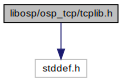
\includegraphics[width=194pt]{tcplib_8h__incl}
\end{center}
\end{figure}
This graph shows which files directly or indirectly include this file\+:\nopagebreak
\begin{figure}[H]
\begin{center}
\leavevmode
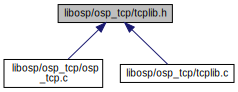
\includegraphics[width=310pt]{tcplib_8h__dep__incl}
\end{center}
\end{figure}
\subsection*{Functions}
\begin{DoxyCompactItemize}
\item 
int \mbox{\hyperlink{tcplib_8h_a82868dec779695fc3eb3e81f32d4df73}{start\+\_\+tcp\+\_\+server}} (int)
\begin{DoxyCompactList}\small\item\em Initiates T\+CP protocol server. \end{DoxyCompactList}\item 
int \mbox{\hyperlink{tcplib_8h_a36c6d89c6b81a745d5cdaaab9262ad9e}{get\+\_\+tcp\+\_\+server\+\_\+connection}} (int)
\begin{DoxyCompactList}\small\item\em Gets T\+CP protocol server. \end{DoxyCompactList}\item 
int \mbox{\hyperlink{tcplib_8h_a5f9d1cbd10cb6fa7dbb71a668d95cacc}{close\+\_\+tcp\+\_\+server\+\_\+connection}} (int)
\begin{DoxyCompactList}\small\item\em Closes T\+CP protocol server. \end{DoxyCompactList}\item 
void \mbox{\hyperlink{tcplib_8h_a363a39459571b78f7c9cb0a825e133c6}{stop\+\_\+tcp\+\_\+server}} (int)
\begin{DoxyCompactList}\small\item\em Stops the T\+CP protocol server. \end{DoxyCompactList}\item 
ssize\+\_\+t \mbox{\hyperlink{tcplib_8h_ab4ed21d70bd1ec9e8302a12ba4ff72c0}{read\+\_\+tcp\+\_\+server\+\_\+stream}} (int, char $\ast$, int)
\begin{DoxyCompactList}\small\item\em Reads data on server side. \end{DoxyCompactList}\item 
int \mbox{\hyperlink{tcplib_8h_af8559d32e146f74f591cbf18122354b5}{start\+\_\+tcp\+\_\+client}} (char $\ast$, int)
\begin{DoxyCompactList}\small\item\em Initiates T\+CP protocol client. \end{DoxyCompactList}\item 
int \mbox{\hyperlink{tcplib_8h_adbad3e70a6ec4e8d0449baac779cef40}{stop\+\_\+tcp\+\_\+client}} (int)
\begin{DoxyCompactList}\small\item\em Stops T\+CP protocol client. \end{DoxyCompactList}\item 
ssize\+\_\+t \mbox{\hyperlink{tcplib_8h_a054e71a22607597f9315b5b8406d2402}{send\+\_\+tcp\+\_\+client\+\_\+data}} (int, char $\ast$, int)
\begin{DoxyCompactList}\small\item\em Sends data on client side. \end{DoxyCompactList}\end{DoxyCompactItemize}


\subsection{Function Documentation}
\mbox{\Hypertarget{tcplib_8h_a5f9d1cbd10cb6fa7dbb71a668d95cacc}\label{tcplib_8h_a5f9d1cbd10cb6fa7dbb71a668d95cacc}} 
\index{tcplib.\+h@{tcplib.\+h}!close\+\_\+tcp\+\_\+server\+\_\+connection@{close\+\_\+tcp\+\_\+server\+\_\+connection}}
\index{close\+\_\+tcp\+\_\+server\+\_\+connection@{close\+\_\+tcp\+\_\+server\+\_\+connection}!tcplib.\+h@{tcplib.\+h}}
\subsubsection{\texorpdfstring{close\+\_\+tcp\+\_\+server\+\_\+connection()}{close\_tcp\_server\_connection()}}
{\footnotesize\ttfamily int close\+\_\+tcp\+\_\+server\+\_\+connection (\begin{DoxyParamCaption}\item[{int}]{ }\end{DoxyParamCaption})}



Closes T\+CP protocol server. 

\mbox{\Hypertarget{tcplib_8h_a36c6d89c6b81a745d5cdaaab9262ad9e}\label{tcplib_8h_a36c6d89c6b81a745d5cdaaab9262ad9e}} 
\index{tcplib.\+h@{tcplib.\+h}!get\+\_\+tcp\+\_\+server\+\_\+connection@{get\+\_\+tcp\+\_\+server\+\_\+connection}}
\index{get\+\_\+tcp\+\_\+server\+\_\+connection@{get\+\_\+tcp\+\_\+server\+\_\+connection}!tcplib.\+h@{tcplib.\+h}}
\subsubsection{\texorpdfstring{get\+\_\+tcp\+\_\+server\+\_\+connection()}{get\_tcp\_server\_connection()}}
{\footnotesize\ttfamily int get\+\_\+tcp\+\_\+server\+\_\+connection (\begin{DoxyParamCaption}\item[{int}]{ }\end{DoxyParamCaption})}



Gets T\+CP protocol server. 

\mbox{\Hypertarget{tcplib_8h_ab4ed21d70bd1ec9e8302a12ba4ff72c0}\label{tcplib_8h_ab4ed21d70bd1ec9e8302a12ba4ff72c0}} 
\index{tcplib.\+h@{tcplib.\+h}!read\+\_\+tcp\+\_\+server\+\_\+stream@{read\+\_\+tcp\+\_\+server\+\_\+stream}}
\index{read\+\_\+tcp\+\_\+server\+\_\+stream@{read\+\_\+tcp\+\_\+server\+\_\+stream}!tcplib.\+h@{tcplib.\+h}}
\subsubsection{\texorpdfstring{read\+\_\+tcp\+\_\+server\+\_\+stream()}{read\_tcp\_server\_stream()}}
{\footnotesize\ttfamily ssize\+\_\+t read\+\_\+tcp\+\_\+server\+\_\+stream (\begin{DoxyParamCaption}\item[{int}]{,  }\item[{char $\ast$}]{,  }\item[{int}]{ }\end{DoxyParamCaption})}



Reads data on server side. 

\mbox{\Hypertarget{tcplib_8h_a054e71a22607597f9315b5b8406d2402}\label{tcplib_8h_a054e71a22607597f9315b5b8406d2402}} 
\index{tcplib.\+h@{tcplib.\+h}!send\+\_\+tcp\+\_\+client\+\_\+data@{send\+\_\+tcp\+\_\+client\+\_\+data}}
\index{send\+\_\+tcp\+\_\+client\+\_\+data@{send\+\_\+tcp\+\_\+client\+\_\+data}!tcplib.\+h@{tcplib.\+h}}
\subsubsection{\texorpdfstring{send\+\_\+tcp\+\_\+client\+\_\+data()}{send\_tcp\_client\_data()}}
{\footnotesize\ttfamily ssize\+\_\+t send\+\_\+tcp\+\_\+client\+\_\+data (\begin{DoxyParamCaption}\item[{int}]{,  }\item[{char $\ast$}]{,  }\item[{int}]{ }\end{DoxyParamCaption})}



Sends data on client side. 

\mbox{\Hypertarget{tcplib_8h_af8559d32e146f74f591cbf18122354b5}\label{tcplib_8h_af8559d32e146f74f591cbf18122354b5}} 
\index{tcplib.\+h@{tcplib.\+h}!start\+\_\+tcp\+\_\+client@{start\+\_\+tcp\+\_\+client}}
\index{start\+\_\+tcp\+\_\+client@{start\+\_\+tcp\+\_\+client}!tcplib.\+h@{tcplib.\+h}}
\subsubsection{\texorpdfstring{start\+\_\+tcp\+\_\+client()}{start\_tcp\_client()}}
{\footnotesize\ttfamily int start\+\_\+tcp\+\_\+client (\begin{DoxyParamCaption}\item[{char $\ast$}]{ip,  }\item[{int}]{port }\end{DoxyParamCaption})}



Initiates T\+CP protocol client. 

Starts the client side socket connection based on I\+N\+ET Internet stream-\/oriented sockets. \mbox{\Hypertarget{tcplib_8h_a82868dec779695fc3eb3e81f32d4df73}\label{tcplib_8h_a82868dec779695fc3eb3e81f32d4df73}} 
\index{tcplib.\+h@{tcplib.\+h}!start\+\_\+tcp\+\_\+server@{start\+\_\+tcp\+\_\+server}}
\index{start\+\_\+tcp\+\_\+server@{start\+\_\+tcp\+\_\+server}!tcplib.\+h@{tcplib.\+h}}
\subsubsection{\texorpdfstring{start\+\_\+tcp\+\_\+server()}{start\_tcp\_server()}}
{\footnotesize\ttfamily int start\+\_\+tcp\+\_\+server (\begin{DoxyParamCaption}\item[{int}]{port }\end{DoxyParamCaption})}



Initiates T\+CP protocol server. 

Initiates T\+CP protocol server. \mbox{\Hypertarget{tcplib_8h_adbad3e70a6ec4e8d0449baac779cef40}\label{tcplib_8h_adbad3e70a6ec4e8d0449baac779cef40}} 
\index{tcplib.\+h@{tcplib.\+h}!stop\+\_\+tcp\+\_\+client@{stop\+\_\+tcp\+\_\+client}}
\index{stop\+\_\+tcp\+\_\+client@{stop\+\_\+tcp\+\_\+client}!tcplib.\+h@{tcplib.\+h}}
\subsubsection{\texorpdfstring{stop\+\_\+tcp\+\_\+client()}{stop\_tcp\_client()}}
{\footnotesize\ttfamily int stop\+\_\+tcp\+\_\+client (\begin{DoxyParamCaption}\item[{int}]{ }\end{DoxyParamCaption})}



Stops T\+CP protocol client. 

\mbox{\Hypertarget{tcplib_8h_a363a39459571b78f7c9cb0a825e133c6}\label{tcplib_8h_a363a39459571b78f7c9cb0a825e133c6}} 
\index{tcplib.\+h@{tcplib.\+h}!stop\+\_\+tcp\+\_\+server@{stop\+\_\+tcp\+\_\+server}}
\index{stop\+\_\+tcp\+\_\+server@{stop\+\_\+tcp\+\_\+server}!tcplib.\+h@{tcplib.\+h}}
\subsubsection{\texorpdfstring{stop\+\_\+tcp\+\_\+server()}{stop\_tcp\_server()}}
{\footnotesize\ttfamily void stop\+\_\+tcp\+\_\+server (\begin{DoxyParamCaption}\item[{int}]{ }\end{DoxyParamCaption})}



Stops the T\+CP protocol server. 


\hypertarget{peak__detect_8c}{}\section{libosp/peak\+\_\+detect/peak\+\_\+detect.c File Reference}
\label{peak__detect_8c}\index{libosp/peak\+\_\+detect/peak\+\_\+detect.\+c@{libosp/peak\+\_\+detect/peak\+\_\+detect.\+c}}
{\ttfamily \#include \char`\"{}peak\+\_\+detect.\+h\char`\"{}}\newline
{\ttfamily \#include $<$math.\+h$>$}\newline
{\ttfamily \#include $<$limits.\+h$>$}\newline
{\ttfamily \#include $<$stdlib.\+h$>$}\newline
{\ttfamily \#include $<$string.\+h$>$}\newline
Include dependency graph for peak\+\_\+detect.\+c\+:\nopagebreak
\begin{figure}[H]
\begin{center}
\leavevmode
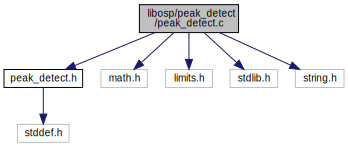
\includegraphics[width=350pt]{peak__detect_8c__incl}
\end{center}
\end{figure}
\subsection*{Data Structures}
\begin{DoxyCompactItemize}
\item 
struct \mbox{\hyperlink{structpeak__detect__t}{peak\+\_\+detect\+\_\+t}}
\begin{DoxyCompactList}\small\item\em Peak Detect data structure. \end{DoxyCompactList}\end{DoxyCompactItemize}
\subsection*{Functions}
\begin{DoxyCompactItemize}
\item 
\mbox{\hyperlink{peak__detect_8h_a152d14cd03f6e1ac947c95921da5507c}{Peak\+\_\+detect}} \mbox{\hyperlink{peak__detect_8c_a1bb9895ff8c4b0457213e526fd4fab74}{peak\+\_\+detect\+\_\+init}} (float fsamp, unsigned int num\+\_\+bands)
\begin{DoxyCompactList}\small\item\em Function to initialize the peak\+\_\+detect data struct. \end{DoxyCompactList}\item 
void \mbox{\hyperlink{peak__detect_8c_a28a24577ab91983936daee15fd88af54}{peak\+\_\+to\+\_\+spl}} (float $\ast$peak, float $\ast$pdb, size\+\_\+t len)
\begin{DoxyCompactList}\small\item\em Function to convert the output from the peak detector into dB S\+PL (Sound Pressure Level). \end{DoxyCompactList}\item 
void \mbox{\hyperlink{peak__detect_8c_a3d0ec744b3cd1bf9acd7598def47748c}{peak\+\_\+detect}} (\mbox{\hyperlink{peak__detect_8h_a152d14cd03f6e1ac947c95921da5507c}{Peak\+\_\+detect}} pd, float $\ast$input, size\+\_\+t len, float $\ast$peak, float attack\+\_\+time, float release\+\_\+time, int band\+\_\+num)
\begin{DoxyCompactList}\small\item\em Function to peak detect the signal. The attack and release times are specified as A\+N\+SI values which are then converted to filter time constants. The peak detector is given by Kates, Eq (8.\+1). \end{DoxyCompactList}\item 
int \mbox{\hyperlink{peak__detect_8c_a0012f353d07e27778b050692205a717e}{peak\+\_\+detect\+\_\+destroy}} (\mbox{\hyperlink{peak__detect_8h_a152d14cd03f6e1ac947c95921da5507c}{Peak\+\_\+detect}} pd)
\begin{DoxyCompactList}\small\item\em Function to close and free the Peak\+\_\+detect instance. \end{DoxyCompactList}\end{DoxyCompactItemize}


\subsection{Function Documentation}
\mbox{\Hypertarget{peak__detect_8c_a3d0ec744b3cd1bf9acd7598def47748c}\label{peak__detect_8c_a3d0ec744b3cd1bf9acd7598def47748c}} 
\index{peak\+\_\+detect.\+c@{peak\+\_\+detect.\+c}!peak\+\_\+detect@{peak\+\_\+detect}}
\index{peak\+\_\+detect@{peak\+\_\+detect}!peak\+\_\+detect.\+c@{peak\+\_\+detect.\+c}}
\subsubsection{\texorpdfstring{peak\+\_\+detect()}{peak\_detect()}}
{\footnotesize\ttfamily void peak\+\_\+detect (\begin{DoxyParamCaption}\item[{\mbox{\hyperlink{peak__detect_8h_a152d14cd03f6e1ac947c95921da5507c}{Peak\+\_\+detect}}}]{pd,  }\item[{float $\ast$}]{input,  }\item[{size\+\_\+t}]{len,  }\item[{float $\ast$}]{peak,  }\item[{float}]{attack\+\_\+time,  }\item[{float}]{release\+\_\+time,  }\item[{int}]{band\+\_\+num }\end{DoxyParamCaption})}



Function to peak detect the signal. The attack and release times are specified as A\+N\+SI values which are then converted to filter time constants. The peak detector is given by Kates, Eq (8.\+1). 

\begin{DoxySeeAlso}{See also}
\mbox{\hyperlink{structpeak__detect__t}{peak\+\_\+detect\+\_\+t}} 
\end{DoxySeeAlso}

\begin{DoxyParams}{Parameters}
{\em pd} & The instance of the Peak\+\_\+detect structure that was returned from peak\+\_\+detect\+\_\+init \\
\hline
{\em input} & Pointer to the signal array at the frequency sub-\/band (output from sub-\/band filtering) \\
\hline
{\em len} & Length of the input signal \\
\hline
{\em peak} & Pointer to the array that will have peak detection output. i.\+e. output from peak\+\_\+detect \\
\hline
{\em attack\+\_\+time} & Attack time in milliseconds \\
\hline
{\em release\+\_\+time} & Release time in milliseconds \\
\hline
{\em band\+\_\+num} & The sub-\/band number that is being operated on. Required to get the prev\+\_\+peak value for that band \\
\hline
\end{DoxyParams}
\mbox{\Hypertarget{peak__detect_8c_a0012f353d07e27778b050692205a717e}\label{peak__detect_8c_a0012f353d07e27778b050692205a717e}} 
\index{peak\+\_\+detect.\+c@{peak\+\_\+detect.\+c}!peak\+\_\+detect\+\_\+destroy@{peak\+\_\+detect\+\_\+destroy}}
\index{peak\+\_\+detect\+\_\+destroy@{peak\+\_\+detect\+\_\+destroy}!peak\+\_\+detect.\+c@{peak\+\_\+detect.\+c}}
\subsubsection{\texorpdfstring{peak\+\_\+detect\+\_\+destroy()}{peak\_detect\_destroy()}}
{\footnotesize\ttfamily int peak\+\_\+detect\+\_\+destroy (\begin{DoxyParamCaption}\item[{\mbox{\hyperlink{peak__detect_8h_a152d14cd03f6e1ac947c95921da5507c}{Peak\+\_\+detect}}}]{pd }\end{DoxyParamCaption})}



Function to close and free the Peak\+\_\+detect instance. 

\begin{DoxySeeAlso}{See also}
\mbox{\hyperlink{structpeak__detect__t}{peak\+\_\+detect\+\_\+t}} 
\end{DoxySeeAlso}

\begin{DoxyParams}{Parameters}
{\em pd} & The instance of the Peak\+\_\+detect structure that was returned from peak\+\_\+detect\+\_\+init \\
\hline
\end{DoxyParams}
\begin{DoxyReturn}{Returns}
0 if successful. -\/1 otherwise 
\end{DoxyReturn}
\mbox{\Hypertarget{peak__detect_8c_a1bb9895ff8c4b0457213e526fd4fab74}\label{peak__detect_8c_a1bb9895ff8c4b0457213e526fd4fab74}} 
\index{peak\+\_\+detect.\+c@{peak\+\_\+detect.\+c}!peak\+\_\+detect\+\_\+init@{peak\+\_\+detect\+\_\+init}}
\index{peak\+\_\+detect\+\_\+init@{peak\+\_\+detect\+\_\+init}!peak\+\_\+detect.\+c@{peak\+\_\+detect.\+c}}
\subsubsection{\texorpdfstring{peak\+\_\+detect\+\_\+init()}{peak\_detect\_init()}}
{\footnotesize\ttfamily \mbox{\hyperlink{peak__detect_8h_a152d14cd03f6e1ac947c95921da5507c}{Peak\+\_\+detect}} peak\+\_\+detect\+\_\+init (\begin{DoxyParamCaption}\item[{float}]{fsamp,  }\item[{unsigned int}]{num\+\_\+bands }\end{DoxyParamCaption})}



Function to initialize the peak\+\_\+detect data struct. 

Allocates memory to the Peak\+\_\+detect instance and initialize its parameters. prev\+\_\+peak is set to zero for all bands for the first time.


\begin{DoxyParams}{Parameters}
{\em fsamp} & Sampling rate in Hz \\
\hline
{\em num\+\_\+bands} & Number of sub-\/bands. Required to store prev\+\_\+peak values for each band \\
\hline
\end{DoxyParams}
\begin{DoxyReturn}{Returns}
Peak\+\_\+detect Returns the Peak\+\_\+detect instance/object if memory is succesfully allocated or returns N\+U\+LL. 
\end{DoxyReturn}
\mbox{\Hypertarget{peak__detect_8c_a28a24577ab91983936daee15fd88af54}\label{peak__detect_8c_a28a24577ab91983936daee15fd88af54}} 
\index{peak\+\_\+detect.\+c@{peak\+\_\+detect.\+c}!peak\+\_\+to\+\_\+spl@{peak\+\_\+to\+\_\+spl}}
\index{peak\+\_\+to\+\_\+spl@{peak\+\_\+to\+\_\+spl}!peak\+\_\+detect.\+c@{peak\+\_\+detect.\+c}}
\subsubsection{\texorpdfstring{peak\+\_\+to\+\_\+spl()}{peak\_to\_spl()}}
{\footnotesize\ttfamily void peak\+\_\+to\+\_\+spl (\begin{DoxyParamCaption}\item[{float $\ast$}]{peak,  }\item[{float $\ast$}]{pdb,  }\item[{size\+\_\+t}]{len }\end{DoxyParamCaption})}



Function to convert the output from the peak detector into dB S\+PL (Sound Pressure Level). 

The S\+PL output will be used by the wide dynamic-\/range compression (wdrc) function. The function assumes that an R\+MS signal value of 1 corresponds to \mbox{\hyperlink{peak__detect_8h_a4f9fe2f1309c3dbfcf132e9fffb11fb2}{D\+E\+F\+A\+U\+L\+T\+\_\+\+L\+E\+V\+E\+L(100)}} dB S\+PL and converts the signal accordingly. The input W\+AV file therefore needs to be set to R\+MS = 1 at the start of processing.


\begin{DoxyParams}{Parameters}
{\em peak} & Pointer to the signal to be conveted to dB S\+PL. i.\+e. the output from the peak\+\_\+detect \\
\hline
{\em pdb} & Pointer to the signal converted to dB S\+PL. i.\+e. the output of peak\+\_\+to\+\_\+spl \\
\hline
{\em len} & Length of the input signal to be converted to dB S\+PL \\
\hline
\end{DoxyParams}

\hypertarget{peak__detect_8h}{}\section{libosp/peak\+\_\+detect/peak\+\_\+detect.h File Reference}
\label{peak__detect_8h}\index{libosp/peak\+\_\+detect/peak\+\_\+detect.\+h@{libosp/peak\+\_\+detect/peak\+\_\+detect.\+h}}
{\ttfamily \#include $<$stddef.\+h$>$}\newline
Include dependency graph for peak\+\_\+detect.\+h\+:\nopagebreak
\begin{figure}[H]
\begin{center}
\leavevmode
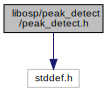
\includegraphics[width=179pt]{peak__detect_8h__incl}
\end{center}
\end{figure}
This graph shows which files directly or indirectly include this file\+:\nopagebreak
\begin{figure}[H]
\begin{center}
\leavevmode
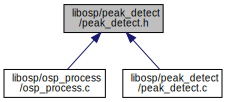
\includegraphics[width=298pt]{peak__detect_8h__dep__incl}
\end{center}
\end{figure}
\subsection*{Macros}
\begin{DoxyCompactItemize}
\item 
\#define \mbox{\hyperlink{peak__detect_8h_ab701824136346377b44fc3adb8050b29}{D\+B\+L\+\_\+\+E\+P\+S\+I\+L\+ON}}~2.\+2204460492503131e-\/16
\begin{DoxyCompactList}\small\item\em Small constant to avoid taking the log of zero. \end{DoxyCompactList}\item 
\#define \mbox{\hyperlink{peak__detect_8h_a4f9fe2f1309c3dbfcf132e9fffb11fb2}{D\+E\+F\+A\+U\+L\+T\+\_\+\+L\+E\+V\+EL}}~(100)
\begin{DoxyCompactList}\small\item\em Default dB S\+PL level corresponding to signal R\+MS value of 1. \end{DoxyCompactList}\end{DoxyCompactItemize}
\subsection*{Typedefs}
\begin{DoxyCompactItemize}
\item 
typedef struct \mbox{\hyperlink{structpeak__detect__t}{peak\+\_\+detect\+\_\+t}} $\ast$ \mbox{\hyperlink{peak__detect_8h_a152d14cd03f6e1ac947c95921da5507c}{Peak\+\_\+detect}}
\end{DoxyCompactItemize}
\subsection*{Functions}
\begin{DoxyCompactItemize}
\item 
\mbox{\hyperlink{peak__detect_8h_a152d14cd03f6e1ac947c95921da5507c}{Peak\+\_\+detect}} \mbox{\hyperlink{peak__detect_8h_a1bb9895ff8c4b0457213e526fd4fab74}{peak\+\_\+detect\+\_\+init}} (float fsamp, unsigned int num\+\_\+bands)
\begin{DoxyCompactList}\small\item\em Function to initialize the peak\+\_\+detect data struct. \end{DoxyCompactList}\item 
void \mbox{\hyperlink{peak__detect_8h_a28a24577ab91983936daee15fd88af54}{peak\+\_\+to\+\_\+spl}} (float $\ast$peak, float $\ast$pdb, size\+\_\+t len)
\begin{DoxyCompactList}\small\item\em Function to convert the output from the peak detector into dB S\+PL (Sound Pressure Level). \end{DoxyCompactList}\item 
void \mbox{\hyperlink{peak__detect_8h_a3d0ec744b3cd1bf9acd7598def47748c}{peak\+\_\+detect}} (\mbox{\hyperlink{peak__detect_8h_a152d14cd03f6e1ac947c95921da5507c}{Peak\+\_\+detect}} pd, float $\ast$input, size\+\_\+t len, float $\ast$peak, float attack\+\_\+time, float release\+\_\+time, int band\+\_\+num)
\begin{DoxyCompactList}\small\item\em Function to peak detect the signal. The attack and release times are specified as A\+N\+SI values which are then converted to filter time constants. The peak detector is given by Kates, Eq (8.\+1). \end{DoxyCompactList}\item 
int \mbox{\hyperlink{peak__detect_8h_a0012f353d07e27778b050692205a717e}{peak\+\_\+detect\+\_\+destroy}} (\mbox{\hyperlink{peak__detect_8h_a152d14cd03f6e1ac947c95921da5507c}{Peak\+\_\+detect}} pd)
\begin{DoxyCompactList}\small\item\em Function to close and free the Peak\+\_\+detect instance. \end{DoxyCompactList}\end{DoxyCompactItemize}


\subsection{Macro Definition Documentation}
\mbox{\Hypertarget{peak__detect_8h_ab701824136346377b44fc3adb8050b29}\label{peak__detect_8h_ab701824136346377b44fc3adb8050b29}} 
\index{peak\+\_\+detect.\+h@{peak\+\_\+detect.\+h}!D\+B\+L\+\_\+\+E\+P\+S\+I\+L\+ON@{D\+B\+L\+\_\+\+E\+P\+S\+I\+L\+ON}}
\index{D\+B\+L\+\_\+\+E\+P\+S\+I\+L\+ON@{D\+B\+L\+\_\+\+E\+P\+S\+I\+L\+ON}!peak\+\_\+detect.\+h@{peak\+\_\+detect.\+h}}
\subsubsection{\texorpdfstring{D\+B\+L\+\_\+\+E\+P\+S\+I\+L\+ON}{DBL\_EPSILON}}
{\footnotesize\ttfamily \#define D\+B\+L\+\_\+\+E\+P\+S\+I\+L\+ON~2.\+2204460492503131e-\/16}



Small constant to avoid taking the log of zero. 

\mbox{\Hypertarget{peak__detect_8h_a4f9fe2f1309c3dbfcf132e9fffb11fb2}\label{peak__detect_8h_a4f9fe2f1309c3dbfcf132e9fffb11fb2}} 
\index{peak\+\_\+detect.\+h@{peak\+\_\+detect.\+h}!D\+E\+F\+A\+U\+L\+T\+\_\+\+L\+E\+V\+EL@{D\+E\+F\+A\+U\+L\+T\+\_\+\+L\+E\+V\+EL}}
\index{D\+E\+F\+A\+U\+L\+T\+\_\+\+L\+E\+V\+EL@{D\+E\+F\+A\+U\+L\+T\+\_\+\+L\+E\+V\+EL}!peak\+\_\+detect.\+h@{peak\+\_\+detect.\+h}}
\subsubsection{\texorpdfstring{D\+E\+F\+A\+U\+L\+T\+\_\+\+L\+E\+V\+EL}{DEFAULT\_LEVEL}}
{\footnotesize\ttfamily \#define D\+E\+F\+A\+U\+L\+T\+\_\+\+L\+E\+V\+EL~(100)}



Default dB S\+PL level corresponding to signal R\+MS value of 1. 



\subsection{Typedef Documentation}
\mbox{\Hypertarget{peak__detect_8h_a152d14cd03f6e1ac947c95921da5507c}\label{peak__detect_8h_a152d14cd03f6e1ac947c95921da5507c}} 
\index{peak\+\_\+detect.\+h@{peak\+\_\+detect.\+h}!Peak\+\_\+detect@{Peak\+\_\+detect}}
\index{Peak\+\_\+detect@{Peak\+\_\+detect}!peak\+\_\+detect.\+h@{peak\+\_\+detect.\+h}}
\subsubsection{\texorpdfstring{Peak\+\_\+detect}{Peak\_detect}}
{\footnotesize\ttfamily typedef struct \mbox{\hyperlink{structpeak__detect__t}{peak\+\_\+detect\+\_\+t}}$\ast$ \mbox{\hyperlink{peak__detect_8h_a152d14cd03f6e1ac947c95921da5507c}{Peak\+\_\+detect}}}



\subsection{Function Documentation}
\mbox{\Hypertarget{peak__detect_8h_a3d0ec744b3cd1bf9acd7598def47748c}\label{peak__detect_8h_a3d0ec744b3cd1bf9acd7598def47748c}} 
\index{peak\+\_\+detect.\+h@{peak\+\_\+detect.\+h}!peak\+\_\+detect@{peak\+\_\+detect}}
\index{peak\+\_\+detect@{peak\+\_\+detect}!peak\+\_\+detect.\+h@{peak\+\_\+detect.\+h}}
\subsubsection{\texorpdfstring{peak\+\_\+detect()}{peak\_detect()}}
{\footnotesize\ttfamily void peak\+\_\+detect (\begin{DoxyParamCaption}\item[{\mbox{\hyperlink{peak__detect_8h_a152d14cd03f6e1ac947c95921da5507c}{Peak\+\_\+detect}}}]{pd,  }\item[{float $\ast$}]{input,  }\item[{size\+\_\+t}]{len,  }\item[{float $\ast$}]{peak,  }\item[{float}]{attack\+\_\+time,  }\item[{float}]{release\+\_\+time,  }\item[{int}]{band\+\_\+num }\end{DoxyParamCaption})}



Function to peak detect the signal. The attack and release times are specified as A\+N\+SI values which are then converted to filter time constants. The peak detector is given by Kates, Eq (8.\+1). 

\begin{DoxySeeAlso}{See also}
\mbox{\hyperlink{structpeak__detect__t}{peak\+\_\+detect\+\_\+t}} 
\end{DoxySeeAlso}

\begin{DoxyParams}{Parameters}
{\em pd} & The instance of the Peak\+\_\+detect structure that was returned from peak\+\_\+detect\+\_\+init \\
\hline
{\em input} & Pointer to the signal array at the frequency sub-\/band (output from sub-\/band filtering) \\
\hline
{\em len} & Length of the input signal \\
\hline
{\em peak} & Pointer to the array that will have peak detection output. i.\+e. output from peak\+\_\+detect \\
\hline
{\em attack\+\_\+time} & Attack time in milliseconds \\
\hline
{\em release\+\_\+time} & Release time in milliseconds \\
\hline
{\em band\+\_\+num} & The sub-\/band number that is being operated on. Required to get the prev\+\_\+peak value for that band \\
\hline
\end{DoxyParams}
\mbox{\Hypertarget{peak__detect_8h_a0012f353d07e27778b050692205a717e}\label{peak__detect_8h_a0012f353d07e27778b050692205a717e}} 
\index{peak\+\_\+detect.\+h@{peak\+\_\+detect.\+h}!peak\+\_\+detect\+\_\+destroy@{peak\+\_\+detect\+\_\+destroy}}
\index{peak\+\_\+detect\+\_\+destroy@{peak\+\_\+detect\+\_\+destroy}!peak\+\_\+detect.\+h@{peak\+\_\+detect.\+h}}
\subsubsection{\texorpdfstring{peak\+\_\+detect\+\_\+destroy()}{peak\_detect\_destroy()}}
{\footnotesize\ttfamily int peak\+\_\+detect\+\_\+destroy (\begin{DoxyParamCaption}\item[{\mbox{\hyperlink{peak__detect_8h_a152d14cd03f6e1ac947c95921da5507c}{Peak\+\_\+detect}}}]{pd }\end{DoxyParamCaption})}



Function to close and free the Peak\+\_\+detect instance. 

\begin{DoxySeeAlso}{See also}
\mbox{\hyperlink{structpeak__detect__t}{peak\+\_\+detect\+\_\+t}} 
\end{DoxySeeAlso}

\begin{DoxyParams}{Parameters}
{\em pd} & The instance of the Peak\+\_\+detect structure that was returned from peak\+\_\+detect\+\_\+init \\
\hline
\end{DoxyParams}
\begin{DoxyReturn}{Returns}
0 if successful. -\/1 otherwise 
\end{DoxyReturn}
\mbox{\Hypertarget{peak__detect_8h_a1bb9895ff8c4b0457213e526fd4fab74}\label{peak__detect_8h_a1bb9895ff8c4b0457213e526fd4fab74}} 
\index{peak\+\_\+detect.\+h@{peak\+\_\+detect.\+h}!peak\+\_\+detect\+\_\+init@{peak\+\_\+detect\+\_\+init}}
\index{peak\+\_\+detect\+\_\+init@{peak\+\_\+detect\+\_\+init}!peak\+\_\+detect.\+h@{peak\+\_\+detect.\+h}}
\subsubsection{\texorpdfstring{peak\+\_\+detect\+\_\+init()}{peak\_detect\_init()}}
{\footnotesize\ttfamily \mbox{\hyperlink{peak__detect_8h_a152d14cd03f6e1ac947c95921da5507c}{Peak\+\_\+detect}} peak\+\_\+detect\+\_\+init (\begin{DoxyParamCaption}\item[{float}]{fsamp,  }\item[{unsigned int}]{num\+\_\+bands }\end{DoxyParamCaption})}



Function to initialize the peak\+\_\+detect data struct. 

Allocates memory to the Peak\+\_\+detect instance and initialize its parameters. prev\+\_\+peak is set to zero for all bands for the first time.


\begin{DoxyParams}{Parameters}
{\em fsamp} & Sampling rate in Hz \\
\hline
{\em num\+\_\+bands} & Number of sub-\/bands. Required to store prev\+\_\+peak values for each band \\
\hline
\end{DoxyParams}
\begin{DoxyReturn}{Returns}
Peak\+\_\+detect Returns the Peak\+\_\+detect instance/object if memory is succesfully allocated or returns N\+U\+LL. 
\end{DoxyReturn}
\mbox{\Hypertarget{peak__detect_8h_a28a24577ab91983936daee15fd88af54}\label{peak__detect_8h_a28a24577ab91983936daee15fd88af54}} 
\index{peak\+\_\+detect.\+h@{peak\+\_\+detect.\+h}!peak\+\_\+to\+\_\+spl@{peak\+\_\+to\+\_\+spl}}
\index{peak\+\_\+to\+\_\+spl@{peak\+\_\+to\+\_\+spl}!peak\+\_\+detect.\+h@{peak\+\_\+detect.\+h}}
\subsubsection{\texorpdfstring{peak\+\_\+to\+\_\+spl()}{peak\_to\_spl()}}
{\footnotesize\ttfamily void peak\+\_\+to\+\_\+spl (\begin{DoxyParamCaption}\item[{float $\ast$}]{peak,  }\item[{float $\ast$}]{pdb,  }\item[{size\+\_\+t}]{len }\end{DoxyParamCaption})}



Function to convert the output from the peak detector into dB S\+PL (Sound Pressure Level). 

The S\+PL output will be used by the wide dynamic-\/range compression (wdrc) function. The function assumes that an R\+MS signal value of 1 corresponds to \mbox{\hyperlink{peak__detect_8h_a4f9fe2f1309c3dbfcf132e9fffb11fb2}{D\+E\+F\+A\+U\+L\+T\+\_\+\+L\+E\+V\+E\+L(100)}} dB S\+PL and converts the signal accordingly. The input W\+AV file therefore needs to be set to R\+MS = 1 at the start of processing.


\begin{DoxyParams}{Parameters}
{\em peak} & Pointer to the signal to be conveted to dB S\+PL. i.\+e. the output from the peak\+\_\+detect \\
\hline
{\em pdb} & Pointer to the signal converted to dB S\+PL. i.\+e. the output of peak\+\_\+to\+\_\+spl \\
\hline
{\em len} & Length of the input signal to be converted to dB S\+PL \\
\hline
\end{DoxyParams}

\hypertarget{resample_8c}{}\section{libosp/resample/resample.c File Reference}
\label{resample_8c}\index{libosp/resample/resample.\+c@{libosp/resample/resample.\+c}}
{\ttfamily \#include $<$stdlib.\+h$>$}\newline
{\ttfamily \#include \char`\"{}resample.\+h\char`\"{}}\newline
{\ttfamily \#include \char`\"{}filter.\+h\char`\"{}}\newline
Include dependency graph for resample.\+c\+:\nopagebreak
\begin{figure}[H]
\begin{center}
\leavevmode
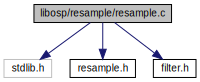
\includegraphics[width=272pt]{resample_8c__incl}
\end{center}
\end{figure}
\subsection*{Data Structures}
\begin{DoxyCompactItemize}
\item 
struct \mbox{\hyperlink{structresample__t}{resample\+\_\+t}}
\begin{DoxyCompactList}\small\item\em Data struct containing variables for resampler. \end{DoxyCompactList}\end{DoxyCompactItemize}
\subsection*{Macros}
\begin{DoxyCompactItemize}
\item 
\#define \mbox{\hyperlink{resample_8c_a6c433fc0ede8da10a34aa7ff3f121b97}{S\+I\+Z\+E\+\_\+32}}~32
\item 
\#define \mbox{\hyperlink{resample_8c_ad9e4c0b5db1080f28b3588c4f4dc749f}{S\+I\+Z\+E\+\_\+48}}~48
\end{DoxyCompactItemize}
\subsection*{Functions}
\begin{DoxyCompactItemize}
\item 
static size\+\_\+t \mbox{\hyperlink{resample_8c_adb271f049edb4d918f3e29ea2142ef0f}{interpolate}} (float $\ast$input, float $\ast$output, size\+\_\+t input\+\_\+len, int int\+\_\+factor)
\item 
static size\+\_\+t \mbox{\hyperlink{resample_8c_acef0bf57e61989b8307c78a1ba693ded}{decimate}} (float $\ast$input, float $\ast$output, size\+\_\+t input\+\_\+len, int dec\+\_\+factor)
\item 
\mbox{\hyperlink{resample_8h_aa18dcb3a00dcbfe35cecd42a27ff3097}{Resample}} \mbox{\hyperlink{resample_8c_ae9df3f5bb638689d2d193913bee84d08}{resample\+\_\+init}} (const float $\ast$upsample\+\_\+taps, int up\+\_\+len, const float $\ast$downsample\+\_\+taps, int down\+\_\+len)
\begin{DoxyCompactList}\small\item\em Initialization function for the resample structure. \end{DoxyCompactList}\item 
size\+\_\+t \mbox{\hyperlink{resample_8c_a268ac02447f54bfd52367bf857acf146}{resample\+\_\+48\+\_\+32}} (\mbox{\hyperlink{resample_8h_aa18dcb3a00dcbfe35cecd42a27ff3097}{Resample}} obj, float $\ast$in\+\_\+48, float $\ast$out\+\_\+32, int size\+\_\+input)
\begin{DoxyCompactList}\small\item\em Resamples an input of 48 samples at 48k\+Hz sampling rate, and resamples it to 32k\+Hz. \end{DoxyCompactList}\item 
size\+\_\+t \mbox{\hyperlink{resample_8c_a1ca7f92bb107bf50a9c3aa3b8bfd375e}{resample\+\_\+32\+\_\+48}} (\mbox{\hyperlink{resample_8h_aa18dcb3a00dcbfe35cecd42a27ff3097}{Resample}} obj, float $\ast$in\+\_\+32, float $\ast$out\+\_\+48, size\+\_\+t size\+\_\+input)
\begin{DoxyCompactList}\small\item\em Resamples an input of 32 samples at 32k\+Hz sampling rate, and resamples it to 48k\+Hz. \end{DoxyCompactList}\item 
size\+\_\+t \mbox{\hyperlink{resample_8c_a4cb21f88698fb352b2740675b0135e58}{resample\+\_\+96\+\_\+32}} (\mbox{\hyperlink{resample_8h_aa18dcb3a00dcbfe35cecd42a27ff3097}{Resample}} obj, float $\ast$in\+\_\+96, float $\ast$out\+\_\+32, size\+\_\+t size\+\_\+input)
\begin{DoxyCompactList}\small\item\em Resamples an input of 96 samples at 96k\+Hz sampling rate, and resamples it to 32k\+Hz. \end{DoxyCompactList}\item 
size\+\_\+t \mbox{\hyperlink{resample_8c_aa33bf7f29f45c3435b6d28af6a1f683e}{resample\+\_\+32\+\_\+96}} (\mbox{\hyperlink{resample_8h_aa18dcb3a00dcbfe35cecd42a27ff3097}{Resample}} obj, float $\ast$in\+\_\+32, float $\ast$out\+\_\+96, size\+\_\+t size\+\_\+input)
\begin{DoxyCompactList}\small\item\em Resamples an input of 32 samples at 32k\+Hz sampling rate, and resamples it to 96k\+Hz. \end{DoxyCompactList}\item 
int \mbox{\hyperlink{resample_8c_ab73f93ef213ac8a2e2b930a3ed616120}{resample\+\_\+destroy}} (\mbox{\hyperlink{resample_8h_aa18dcb3a00dcbfe35cecd42a27ff3097}{Resample}} obj)
\begin{DoxyCompactList}\small\item\em Frees the Resample struct. \end{DoxyCompactList}\end{DoxyCompactItemize}


\subsection{Macro Definition Documentation}
\mbox{\Hypertarget{resample_8c_a6c433fc0ede8da10a34aa7ff3f121b97}\label{resample_8c_a6c433fc0ede8da10a34aa7ff3f121b97}} 
\index{resample.\+c@{resample.\+c}!S\+I\+Z\+E\+\_\+32@{S\+I\+Z\+E\+\_\+32}}
\index{S\+I\+Z\+E\+\_\+32@{S\+I\+Z\+E\+\_\+32}!resample.\+c@{resample.\+c}}
\subsubsection{\texorpdfstring{S\+I\+Z\+E\+\_\+32}{SIZE\_32}}
{\footnotesize\ttfamily \#define S\+I\+Z\+E\+\_\+32~32}

\mbox{\Hypertarget{resample_8c_ad9e4c0b5db1080f28b3588c4f4dc749f}\label{resample_8c_ad9e4c0b5db1080f28b3588c4f4dc749f}} 
\index{resample.\+c@{resample.\+c}!S\+I\+Z\+E\+\_\+48@{S\+I\+Z\+E\+\_\+48}}
\index{S\+I\+Z\+E\+\_\+48@{S\+I\+Z\+E\+\_\+48}!resample.\+c@{resample.\+c}}
\subsubsection{\texorpdfstring{S\+I\+Z\+E\+\_\+48}{SIZE\_48}}
{\footnotesize\ttfamily \#define S\+I\+Z\+E\+\_\+48~48}



\subsection{Function Documentation}
\mbox{\Hypertarget{resample_8c_acef0bf57e61989b8307c78a1ba693ded}\label{resample_8c_acef0bf57e61989b8307c78a1ba693ded}} 
\index{resample.\+c@{resample.\+c}!decimate@{decimate}}
\index{decimate@{decimate}!resample.\+c@{resample.\+c}}
\subsubsection{\texorpdfstring{decimate()}{decimate()}}
{\footnotesize\ttfamily static size\+\_\+t decimate (\begin{DoxyParamCaption}\item[{float $\ast$}]{input,  }\item[{float $\ast$}]{output,  }\item[{size\+\_\+t}]{input\+\_\+len,  }\item[{int}]{dec\+\_\+factor }\end{DoxyParamCaption})\hspace{0.3cm}{\ttfamily [static]}}

\mbox{\Hypertarget{resample_8c_adb271f049edb4d918f3e29ea2142ef0f}\label{resample_8c_adb271f049edb4d918f3e29ea2142ef0f}} 
\index{resample.\+c@{resample.\+c}!interpolate@{interpolate}}
\index{interpolate@{interpolate}!resample.\+c@{resample.\+c}}
\subsubsection{\texorpdfstring{interpolate()}{interpolate()}}
{\footnotesize\ttfamily static size\+\_\+t interpolate (\begin{DoxyParamCaption}\item[{float $\ast$}]{input,  }\item[{float $\ast$}]{output,  }\item[{size\+\_\+t}]{input\+\_\+len,  }\item[{int}]{int\+\_\+factor }\end{DoxyParamCaption})\hspace{0.3cm}{\ttfamily [static]}}

\mbox{\Hypertarget{resample_8c_a1ca7f92bb107bf50a9c3aa3b8bfd375e}\label{resample_8c_a1ca7f92bb107bf50a9c3aa3b8bfd375e}} 
\index{resample.\+c@{resample.\+c}!resample\+\_\+32\+\_\+48@{resample\+\_\+32\+\_\+48}}
\index{resample\+\_\+32\+\_\+48@{resample\+\_\+32\+\_\+48}!resample.\+c@{resample.\+c}}
\subsubsection{\texorpdfstring{resample\+\_\+32\+\_\+48()}{resample\_32\_48()}}
{\footnotesize\ttfamily size\+\_\+t resample\+\_\+32\+\_\+48 (\begin{DoxyParamCaption}\item[{\mbox{\hyperlink{resample_8h_aa18dcb3a00dcbfe35cecd42a27ff3097}{Resample}}}]{obj,  }\item[{float $\ast$}]{in\+\_\+32,  }\item[{float $\ast$}]{out\+\_\+48,  }\item[{size\+\_\+t}]{size\+\_\+input }\end{DoxyParamCaption})}



Resamples an input of 32 samples at 32k\+Hz sampling rate, and resamples it to 48k\+Hz. 


\begin{DoxyParams}{Parameters}
{\em obj} & Resample struct \\
\hline
{\em in\+\_\+32} & Input array of float samples. Must be 32 elements long \\
\hline
{\em out\+\_\+48} & Outout array of float samples. Must be allocated to be 48 elements long. \\
\hline
{\em size\+\_\+input} & The size of the in\+\_\+32 array. This is tested internally and must be 32, or else -\/1 is returned. \\
\hline
\end{DoxyParams}
\mbox{\Hypertarget{resample_8c_aa33bf7f29f45c3435b6d28af6a1f683e}\label{resample_8c_aa33bf7f29f45c3435b6d28af6a1f683e}} 
\index{resample.\+c@{resample.\+c}!resample\+\_\+32\+\_\+96@{resample\+\_\+32\+\_\+96}}
\index{resample\+\_\+32\+\_\+96@{resample\+\_\+32\+\_\+96}!resample.\+c@{resample.\+c}}
\subsubsection{\texorpdfstring{resample\+\_\+32\+\_\+96()}{resample\_32\_96()}}
{\footnotesize\ttfamily size\+\_\+t resample\+\_\+32\+\_\+96 (\begin{DoxyParamCaption}\item[{\mbox{\hyperlink{resample_8h_aa18dcb3a00dcbfe35cecd42a27ff3097}{Resample}}}]{obj,  }\item[{float $\ast$}]{in\+\_\+32,  }\item[{float $\ast$}]{out\+\_\+96,  }\item[{size\+\_\+t}]{size\+\_\+input }\end{DoxyParamCaption})}



Resamples an input of 32 samples at 32k\+Hz sampling rate, and resamples it to 96k\+Hz. 


\begin{DoxyParams}{Parameters}
{\em obj} & Resample struct \\
\hline
{\em in\+\_\+32} & Input array of float samples. Must be 32 elements long \\
\hline
{\em out\+\_\+96} & Outout array of float samples. Must be allocated to be 96 elements long. \\
\hline
{\em size\+\_\+input} & The size of the in\+\_\+32 array. This is tested internally and must be 32, or else -\/1 is returned. \\
\hline
\end{DoxyParams}
\mbox{\Hypertarget{resample_8c_a268ac02447f54bfd52367bf857acf146}\label{resample_8c_a268ac02447f54bfd52367bf857acf146}} 
\index{resample.\+c@{resample.\+c}!resample\+\_\+48\+\_\+32@{resample\+\_\+48\+\_\+32}}
\index{resample\+\_\+48\+\_\+32@{resample\+\_\+48\+\_\+32}!resample.\+c@{resample.\+c}}
\subsubsection{\texorpdfstring{resample\+\_\+48\+\_\+32()}{resample\_48\_32()}}
{\footnotesize\ttfamily size\+\_\+t resample\+\_\+48\+\_\+32 (\begin{DoxyParamCaption}\item[{\mbox{\hyperlink{resample_8h_aa18dcb3a00dcbfe35cecd42a27ff3097}{Resample}}}]{obj,  }\item[{float $\ast$}]{in\+\_\+48,  }\item[{float $\ast$}]{out\+\_\+32,  }\item[{int}]{size\+\_\+input }\end{DoxyParamCaption})}



Resamples an input of 48 samples at 48k\+Hz sampling rate, and resamples it to 32k\+Hz. 


\begin{DoxyParams}{Parameters}
{\em obj} & Resample struct \\
\hline
{\em in\+\_\+48} & Input array of float samples. Must be 48 elements long \\
\hline
{\em out\+\_\+32} & Outout array of float samples. Must be allocated to be 32 elements long. \\
\hline
{\em size\+\_\+input} & The size of the in\+\_\+48 array. This is tested internally and must be 48, or else -\/1 is returned. \\
\hline
\end{DoxyParams}
\mbox{\Hypertarget{resample_8c_a4cb21f88698fb352b2740675b0135e58}\label{resample_8c_a4cb21f88698fb352b2740675b0135e58}} 
\index{resample.\+c@{resample.\+c}!resample\+\_\+96\+\_\+32@{resample\+\_\+96\+\_\+32}}
\index{resample\+\_\+96\+\_\+32@{resample\+\_\+96\+\_\+32}!resample.\+c@{resample.\+c}}
\subsubsection{\texorpdfstring{resample\+\_\+96\+\_\+32()}{resample\_96\_32()}}
{\footnotesize\ttfamily size\+\_\+t resample\+\_\+96\+\_\+32 (\begin{DoxyParamCaption}\item[{\mbox{\hyperlink{resample_8h_aa18dcb3a00dcbfe35cecd42a27ff3097}{Resample}}}]{obj,  }\item[{float $\ast$}]{in\+\_\+96,  }\item[{float $\ast$}]{out\+\_\+32,  }\item[{size\+\_\+t}]{size\+\_\+input }\end{DoxyParamCaption})}



Resamples an input of 96 samples at 96k\+Hz sampling rate, and resamples it to 32k\+Hz. 


\begin{DoxyParams}{Parameters}
{\em obj} & Resample struct \\
\hline
{\em in\+\_\+96} & Input array of float samples. Must be 96 elements long \\
\hline
{\em out\+\_\+32} & Outout array of float samples. Must be allocated to be 32 elements long. \\
\hline
{\em size\+\_\+input} & The size of the in\+\_\+96 array. This is tested internally and must be 96, or else -\/1 is returned. \\
\hline
\end{DoxyParams}
\mbox{\Hypertarget{resample_8c_ab73f93ef213ac8a2e2b930a3ed616120}\label{resample_8c_ab73f93ef213ac8a2e2b930a3ed616120}} 
\index{resample.\+c@{resample.\+c}!resample\+\_\+destroy@{resample\+\_\+destroy}}
\index{resample\+\_\+destroy@{resample\+\_\+destroy}!resample.\+c@{resample.\+c}}
\subsubsection{\texorpdfstring{resample\+\_\+destroy()}{resample\_destroy()}}
{\footnotesize\ttfamily int resample\+\_\+destroy (\begin{DoxyParamCaption}\item[{\mbox{\hyperlink{resample_8h_aa18dcb3a00dcbfe35cecd42a27ff3097}{Resample}}}]{obj }\end{DoxyParamCaption})}



Frees the Resample struct. 


\begin{DoxyParams}{Parameters}
{\em obj} & Resample struct \\
\hline
\end{DoxyParams}
\begin{DoxyReturn}{Returns}
Returns 0 on success, -\/1 on error 
\end{DoxyReturn}
\mbox{\Hypertarget{resample_8c_ae9df3f5bb638689d2d193913bee84d08}\label{resample_8c_ae9df3f5bb638689d2d193913bee84d08}} 
\index{resample.\+c@{resample.\+c}!resample\+\_\+init@{resample\+\_\+init}}
\index{resample\+\_\+init@{resample\+\_\+init}!resample.\+c@{resample.\+c}}
\subsubsection{\texorpdfstring{resample\+\_\+init()}{resample\_init()}}
{\footnotesize\ttfamily \mbox{\hyperlink{resample_8h_aa18dcb3a00dcbfe35cecd42a27ff3097}{Resample}} resample\+\_\+init (\begin{DoxyParamCaption}\item[{const float $\ast$}]{upsample\+\_\+taps,  }\item[{int}]{up\+\_\+len,  }\item[{const float $\ast$}]{downsample\+\_\+taps,  }\item[{int}]{down\+\_\+len }\end{DoxyParamCaption})}



Initialization function for the resample structure. 

\begin{DoxySeeAlso}{See also}
\mbox{\hyperlink{structresample__t}{resample\+\_\+t}} 
\end{DoxySeeAlso}

\begin{DoxyParams}{Parameters}
{\em upsample\+\_\+taps} & The taps of the filter to be filtered with the input after being interpolated \\
\hline
{\em up\+\_\+len} & Length of upsample filter \\
\hline
{\em downsample\+\_\+taps} & The taps of the filter to be filtered with the signal before being decimated \\
\hline
{\em down\+\_\+len} & Length of the downsample filter\\
\hline
\end{DoxyParams}
\begin{DoxyReturn}{Returns}
Returns the allocated instance of the O\+SP T\+CP layer data structure (\char`\"{}object\char`\"{} 
\end{DoxyReturn}

\hypertarget{resample_8h}{}\section{libosp/resample/resample.h File Reference}
\label{resample_8h}\index{libosp/resample/resample.\+h@{libosp/resample/resample.\+h}}
This graph shows which files directly or indirectly include this file\+:\nopagebreak
\begin{figure}[H]
\begin{center}
\leavevmode
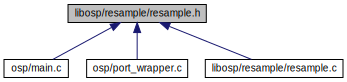
\includegraphics[width=350pt]{resample_8h__dep__incl}
\end{center}
\end{figure}
\subsection*{Typedefs}
\begin{DoxyCompactItemize}
\item 
typedef struct \mbox{\hyperlink{structresample__t}{resample\+\_\+t}} $\ast$ \mbox{\hyperlink{resample_8h_aa18dcb3a00dcbfe35cecd42a27ff3097}{Resample}}
\end{DoxyCompactItemize}
\subsection*{Functions}
\begin{DoxyCompactItemize}
\item 
\mbox{\hyperlink{resample_8h_aa18dcb3a00dcbfe35cecd42a27ff3097}{Resample}} \mbox{\hyperlink{resample_8h_ae9df3f5bb638689d2d193913bee84d08}{resample\+\_\+init}} (const float $\ast$upsample\+\_\+taps, int up\+\_\+len, const float $\ast$downsample\+\_\+taps, int down\+\_\+len)
\begin{DoxyCompactList}\small\item\em Initialization function for the resample structure. \end{DoxyCompactList}\item 
size\+\_\+t \mbox{\hyperlink{resample_8h_a1ca7f92bb107bf50a9c3aa3b8bfd375e}{resample\+\_\+32\+\_\+48}} (\mbox{\hyperlink{resample_8h_aa18dcb3a00dcbfe35cecd42a27ff3097}{Resample}} obj, float $\ast$in\+\_\+32, float $\ast$out\+\_\+48, size\+\_\+t size\+\_\+input)
\begin{DoxyCompactList}\small\item\em Resamples an input of 32 samples at 32k\+Hz sampling rate, and resamples it to 48k\+Hz. \end{DoxyCompactList}\item 
size\+\_\+t \mbox{\hyperlink{resample_8h_a268ac02447f54bfd52367bf857acf146}{resample\+\_\+48\+\_\+32}} (\mbox{\hyperlink{resample_8h_aa18dcb3a00dcbfe35cecd42a27ff3097}{Resample}} obj, float $\ast$in\+\_\+48, float $\ast$out\+\_\+32, int size\+\_\+input)
\begin{DoxyCompactList}\small\item\em Resamples an input of 48 samples at 48k\+Hz sampling rate, and resamples it to 32k\+Hz. \end{DoxyCompactList}\item 
size\+\_\+t \mbox{\hyperlink{resample_8h_a4cb21f88698fb352b2740675b0135e58}{resample\+\_\+96\+\_\+32}} (\mbox{\hyperlink{resample_8h_aa18dcb3a00dcbfe35cecd42a27ff3097}{Resample}} obj, float $\ast$in\+\_\+96, float $\ast$out\+\_\+32, size\+\_\+t size\+\_\+input)
\begin{DoxyCompactList}\small\item\em Resamples an input of 96 samples at 96k\+Hz sampling rate, and resamples it to 32k\+Hz. \end{DoxyCompactList}\item 
size\+\_\+t \mbox{\hyperlink{resample_8h_aa33bf7f29f45c3435b6d28af6a1f683e}{resample\+\_\+32\+\_\+96}} (\mbox{\hyperlink{resample_8h_aa18dcb3a00dcbfe35cecd42a27ff3097}{Resample}} obj, float $\ast$in\+\_\+32, float $\ast$out\+\_\+96, size\+\_\+t size\+\_\+input)
\begin{DoxyCompactList}\small\item\em Resamples an input of 32 samples at 32k\+Hz sampling rate, and resamples it to 96k\+Hz. \end{DoxyCompactList}\item 
int \mbox{\hyperlink{resample_8h_ab73f93ef213ac8a2e2b930a3ed616120}{resample\+\_\+destroy}} (\mbox{\hyperlink{resample_8h_aa18dcb3a00dcbfe35cecd42a27ff3097}{Resample}} obj)
\begin{DoxyCompactList}\small\item\em Frees the Resample struct. \end{DoxyCompactList}\end{DoxyCompactItemize}


\subsection{Typedef Documentation}
\mbox{\Hypertarget{resample_8h_aa18dcb3a00dcbfe35cecd42a27ff3097}\label{resample_8h_aa18dcb3a00dcbfe35cecd42a27ff3097}} 
\index{resample.\+h@{resample.\+h}!Resample@{Resample}}
\index{Resample@{Resample}!resample.\+h@{resample.\+h}}
\subsubsection{\texorpdfstring{Resample}{Resample}}
{\footnotesize\ttfamily typedef struct \mbox{\hyperlink{structresample__t}{resample\+\_\+t}}$\ast$ \mbox{\hyperlink{resample_8h_aa18dcb3a00dcbfe35cecd42a27ff3097}{Resample}}}



\subsection{Function Documentation}
\mbox{\Hypertarget{resample_8h_a1ca7f92bb107bf50a9c3aa3b8bfd375e}\label{resample_8h_a1ca7f92bb107bf50a9c3aa3b8bfd375e}} 
\index{resample.\+h@{resample.\+h}!resample\+\_\+32\+\_\+48@{resample\+\_\+32\+\_\+48}}
\index{resample\+\_\+32\+\_\+48@{resample\+\_\+32\+\_\+48}!resample.\+h@{resample.\+h}}
\subsubsection{\texorpdfstring{resample\+\_\+32\+\_\+48()}{resample\_32\_48()}}
{\footnotesize\ttfamily size\+\_\+t resample\+\_\+32\+\_\+48 (\begin{DoxyParamCaption}\item[{\mbox{\hyperlink{resample_8h_aa18dcb3a00dcbfe35cecd42a27ff3097}{Resample}}}]{obj,  }\item[{float $\ast$}]{in\+\_\+32,  }\item[{float $\ast$}]{out\+\_\+48,  }\item[{size\+\_\+t}]{size\+\_\+input }\end{DoxyParamCaption})}



Resamples an input of 32 samples at 32k\+Hz sampling rate, and resamples it to 48k\+Hz. 


\begin{DoxyParams}{Parameters}
{\em obj} & Resample struct \\
\hline
{\em in\+\_\+32} & Input array of float samples. Must be 32 elements long \\
\hline
{\em out\+\_\+48} & Outout array of float samples. Must be allocated to be 48 elements long. \\
\hline
{\em size\+\_\+input} & The size of the in\+\_\+32 array. This is tested internally and must be 32, or else -\/1 is returned. \\
\hline
\end{DoxyParams}
\mbox{\Hypertarget{resample_8h_aa33bf7f29f45c3435b6d28af6a1f683e}\label{resample_8h_aa33bf7f29f45c3435b6d28af6a1f683e}} 
\index{resample.\+h@{resample.\+h}!resample\+\_\+32\+\_\+96@{resample\+\_\+32\+\_\+96}}
\index{resample\+\_\+32\+\_\+96@{resample\+\_\+32\+\_\+96}!resample.\+h@{resample.\+h}}
\subsubsection{\texorpdfstring{resample\+\_\+32\+\_\+96()}{resample\_32\_96()}}
{\footnotesize\ttfamily size\+\_\+t resample\+\_\+32\+\_\+96 (\begin{DoxyParamCaption}\item[{\mbox{\hyperlink{resample_8h_aa18dcb3a00dcbfe35cecd42a27ff3097}{Resample}}}]{obj,  }\item[{float $\ast$}]{in\+\_\+32,  }\item[{float $\ast$}]{out\+\_\+96,  }\item[{size\+\_\+t}]{size\+\_\+input }\end{DoxyParamCaption})}



Resamples an input of 32 samples at 32k\+Hz sampling rate, and resamples it to 96k\+Hz. 


\begin{DoxyParams}{Parameters}
{\em obj} & Resample struct \\
\hline
{\em in\+\_\+32} & Input array of float samples. Must be 32 elements long \\
\hline
{\em out\+\_\+96} & Outout array of float samples. Must be allocated to be 96 elements long. \\
\hline
{\em size\+\_\+input} & The size of the in\+\_\+32 array. This is tested internally and must be 32, or else -\/1 is returned. \\
\hline
\end{DoxyParams}
\mbox{\Hypertarget{resample_8h_a268ac02447f54bfd52367bf857acf146}\label{resample_8h_a268ac02447f54bfd52367bf857acf146}} 
\index{resample.\+h@{resample.\+h}!resample\+\_\+48\+\_\+32@{resample\+\_\+48\+\_\+32}}
\index{resample\+\_\+48\+\_\+32@{resample\+\_\+48\+\_\+32}!resample.\+h@{resample.\+h}}
\subsubsection{\texorpdfstring{resample\+\_\+48\+\_\+32()}{resample\_48\_32()}}
{\footnotesize\ttfamily size\+\_\+t resample\+\_\+48\+\_\+32 (\begin{DoxyParamCaption}\item[{\mbox{\hyperlink{resample_8h_aa18dcb3a00dcbfe35cecd42a27ff3097}{Resample}}}]{obj,  }\item[{float $\ast$}]{in\+\_\+48,  }\item[{float $\ast$}]{out\+\_\+32,  }\item[{int}]{size\+\_\+input }\end{DoxyParamCaption})}



Resamples an input of 48 samples at 48k\+Hz sampling rate, and resamples it to 32k\+Hz. 


\begin{DoxyParams}{Parameters}
{\em obj} & Resample struct \\
\hline
{\em in\+\_\+48} & Input array of float samples. Must be 48 elements long \\
\hline
{\em out\+\_\+32} & Outout array of float samples. Must be allocated to be 32 elements long. \\
\hline
{\em size\+\_\+input} & The size of the in\+\_\+48 array. This is tested internally and must be 48, or else -\/1 is returned. \\
\hline
\end{DoxyParams}
\mbox{\Hypertarget{resample_8h_a4cb21f88698fb352b2740675b0135e58}\label{resample_8h_a4cb21f88698fb352b2740675b0135e58}} 
\index{resample.\+h@{resample.\+h}!resample\+\_\+96\+\_\+32@{resample\+\_\+96\+\_\+32}}
\index{resample\+\_\+96\+\_\+32@{resample\+\_\+96\+\_\+32}!resample.\+h@{resample.\+h}}
\subsubsection{\texorpdfstring{resample\+\_\+96\+\_\+32()}{resample\_96\_32()}}
{\footnotesize\ttfamily size\+\_\+t resample\+\_\+96\+\_\+32 (\begin{DoxyParamCaption}\item[{\mbox{\hyperlink{resample_8h_aa18dcb3a00dcbfe35cecd42a27ff3097}{Resample}}}]{obj,  }\item[{float $\ast$}]{in\+\_\+96,  }\item[{float $\ast$}]{out\+\_\+32,  }\item[{size\+\_\+t}]{size\+\_\+input }\end{DoxyParamCaption})}



Resamples an input of 96 samples at 96k\+Hz sampling rate, and resamples it to 32k\+Hz. 


\begin{DoxyParams}{Parameters}
{\em obj} & Resample struct \\
\hline
{\em in\+\_\+96} & Input array of float samples. Must be 96 elements long \\
\hline
{\em out\+\_\+32} & Outout array of float samples. Must be allocated to be 32 elements long. \\
\hline
{\em size\+\_\+input} & The size of the in\+\_\+96 array. This is tested internally and must be 96, or else -\/1 is returned. \\
\hline
\end{DoxyParams}
\mbox{\Hypertarget{resample_8h_ab73f93ef213ac8a2e2b930a3ed616120}\label{resample_8h_ab73f93ef213ac8a2e2b930a3ed616120}} 
\index{resample.\+h@{resample.\+h}!resample\+\_\+destroy@{resample\+\_\+destroy}}
\index{resample\+\_\+destroy@{resample\+\_\+destroy}!resample.\+h@{resample.\+h}}
\subsubsection{\texorpdfstring{resample\+\_\+destroy()}{resample\_destroy()}}
{\footnotesize\ttfamily int resample\+\_\+destroy (\begin{DoxyParamCaption}\item[{\mbox{\hyperlink{resample_8h_aa18dcb3a00dcbfe35cecd42a27ff3097}{Resample}}}]{obj }\end{DoxyParamCaption})}



Frees the Resample struct. 


\begin{DoxyParams}{Parameters}
{\em obj} & Resample struct \\
\hline
\end{DoxyParams}
\begin{DoxyReturn}{Returns}
Returns 0 on success, -\/1 on error 
\end{DoxyReturn}
\mbox{\Hypertarget{resample_8h_ae9df3f5bb638689d2d193913bee84d08}\label{resample_8h_ae9df3f5bb638689d2d193913bee84d08}} 
\index{resample.\+h@{resample.\+h}!resample\+\_\+init@{resample\+\_\+init}}
\index{resample\+\_\+init@{resample\+\_\+init}!resample.\+h@{resample.\+h}}
\subsubsection{\texorpdfstring{resample\+\_\+init()}{resample\_init()}}
{\footnotesize\ttfamily \mbox{\hyperlink{resample_8h_aa18dcb3a00dcbfe35cecd42a27ff3097}{Resample}} resample\+\_\+init (\begin{DoxyParamCaption}\item[{const float $\ast$}]{upsample\+\_\+taps,  }\item[{int}]{up\+\_\+len,  }\item[{const float $\ast$}]{downsample\+\_\+taps,  }\item[{int}]{down\+\_\+len }\end{DoxyParamCaption})}



Initialization function for the resample structure. 

\begin{DoxySeeAlso}{See also}
\mbox{\hyperlink{structresample__t}{resample\+\_\+t}} 
\end{DoxySeeAlso}

\begin{DoxyParams}{Parameters}
{\em upsample\+\_\+taps} & The taps of the filter to be filtered with the input after being interpolated \\
\hline
{\em up\+\_\+len} & Length of upsample filter \\
\hline
{\em downsample\+\_\+taps} & The taps of the filter to be filtered with the signal before being decimated \\
\hline
{\em down\+\_\+len} & Length of the downsample filter\\
\hline
\end{DoxyParams}
\begin{DoxyReturn}{Returns}
Returns the allocated instance of the O\+SP T\+CP layer data structure (\char`\"{}object\char`\"{} 
\end{DoxyReturn}

\hypertarget{speech__enhancement_8c}{}\section{libosp/speech\+\_\+enhancement/speech\+\_\+enhancement.c File Reference}
\label{speech__enhancement_8c}\index{libosp/speech\+\_\+enhancement/speech\+\_\+enhancement.\+c@{libosp/speech\+\_\+enhancement/speech\+\_\+enhancement.\+c}}
{\ttfamily \#include \char`\"{}speech\+\_\+enhancement.\+h\char`\"{}}\newline
{\ttfamily \#include $<$math.\+h$>$}\newline
{\ttfamily \#include $<$stdlib.\+h$>$}\newline
{\ttfamily \#include \char`\"{}array\+\_\+utilities.\+h\char`\"{}}\newline
{\ttfamily \#include $<$stdio.\+h$>$}\newline
Include dependency graph for speech\+\_\+enhancement.\+c\+:\nopagebreak
\begin{figure}[H]
\begin{center}
\leavevmode
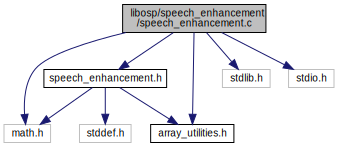
\includegraphics[width=350pt]{speech__enhancement_8c__incl}
\end{center}
\end{figure}
\subsection*{Functions}
\begin{DoxyCompactItemize}
\item 
void \mbox{\hyperlink{speech__enhancement_8c_af3e1113f20ff6a4e412510ed3941cbd8}{speech\+\_\+enhancement}} (float $\ast$input, int ntype, int stype, float sparam, size\+\_\+t len, int fsamp, float $\ast$out)
\end{DoxyCompactItemize}


\subsection{Function Documentation}
\mbox{\Hypertarget{speech__enhancement_8c_af3e1113f20ff6a4e412510ed3941cbd8}\label{speech__enhancement_8c_af3e1113f20ff6a4e412510ed3941cbd8}} 
\index{speech\+\_\+enhancement.\+c@{speech\+\_\+enhancement.\+c}!speech\+\_\+enhancement@{speech\+\_\+enhancement}}
\index{speech\+\_\+enhancement@{speech\+\_\+enhancement}!speech\+\_\+enhancement.\+c@{speech\+\_\+enhancement.\+c}}
\subsubsection{\texorpdfstring{speech\+\_\+enhancement()}{speech\_enhancement()}}
{\footnotesize\ttfamily void speech\+\_\+enhancement (\begin{DoxyParamCaption}\item[{float $\ast$}]{input,  }\item[{int}]{ntype,  }\item[{int}]{stype,  }\item[{float}]{sparam,  }\item[{size\+\_\+t}]{len,  }\item[{int}]{fsamp,  }\item[{float $\ast$}]{out }\end{DoxyParamCaption})}


\hypertarget{speech__enhancement_8h}{}\section{libosp/speech\+\_\+enhancement/speech\+\_\+enhancement.h File Reference}
\label{speech__enhancement_8h}\index{libosp/speech\+\_\+enhancement/speech\+\_\+enhancement.\+h@{libosp/speech\+\_\+enhancement/speech\+\_\+enhancement.\+h}}
{\ttfamily \#include $<$math.\+h$>$}\newline
{\ttfamily \#include $<$stddef.\+h$>$}\newline
{\ttfamily \#include \char`\"{}array\+\_\+utilities.\+h\char`\"{}}\newline
Include dependency graph for speech\+\_\+enhancement.\+h\+:\nopagebreak
\begin{figure}[H]
\begin{center}
\leavevmode
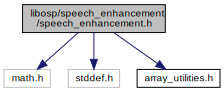
\includegraphics[width=297pt]{speech__enhancement_8h__incl}
\end{center}
\end{figure}
This graph shows which files directly or indirectly include this file\+:\nopagebreak
\begin{figure}[H]
\begin{center}
\leavevmode
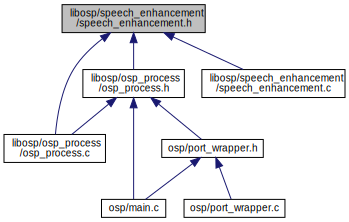
\includegraphics[width=350pt]{speech__enhancement_8h__dep__incl}
\end{center}
\end{figure}
\subsection*{Functions}
\begin{DoxyCompactItemize}
\item 
void \mbox{\hyperlink{speech__enhancement_8h_af3e1113f20ff6a4e412510ed3941cbd8}{speech\+\_\+enhancement}} (float $\ast$input, int ntype, int stype, float sparam, size\+\_\+t len, int fsamp, float $\ast$out)
\end{DoxyCompactItemize}


\subsection{Function Documentation}
\mbox{\Hypertarget{speech__enhancement_8h_af3e1113f20ff6a4e412510ed3941cbd8}\label{speech__enhancement_8h_af3e1113f20ff6a4e412510ed3941cbd8}} 
\index{speech\+\_\+enhancement.\+h@{speech\+\_\+enhancement.\+h}!speech\+\_\+enhancement@{speech\+\_\+enhancement}}
\index{speech\+\_\+enhancement@{speech\+\_\+enhancement}!speech\+\_\+enhancement.\+h@{speech\+\_\+enhancement.\+h}}
\subsubsection{\texorpdfstring{speech\+\_\+enhancement()}{speech\_enhancement()}}
{\footnotesize\ttfamily void speech\+\_\+enhancement (\begin{DoxyParamCaption}\item[{float $\ast$}]{input,  }\item[{int}]{ntype,  }\item[{int}]{stype,  }\item[{float}]{sparam,  }\item[{size\+\_\+t}]{len,  }\item[{int}]{fsamp,  }\item[{float $\ast$}]{out }\end{DoxyParamCaption})}


\hypertarget{mpo_8c}{}\section{libosp/wdrc/mpo.c File Reference}
\label{mpo_8c}\index{libosp/wdrc/mpo.\+c@{libosp/wdrc/mpo.\+c}}
{\ttfamily \#include \char`\"{}mpo.\+h\char`\"{}}\newline
{\ttfamily \#include $<$math.\+h$>$}\newline
Include dependency graph for mpo.\+c\+:\nopagebreak
\begin{figure}[H]
\begin{center}
\leavevmode
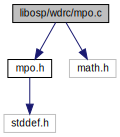
\includegraphics[width=192pt]{mpo_8c__incl}
\end{center}
\end{figure}
\subsection*{Functions}
\begin{DoxyCompactItemize}
\item 
void \mbox{\hyperlink{mpo_8c_ae1fe3ef6535fbf9476ee597f411114c9}{mpo}} (float $\ast$input, float $\ast$pdB, float $\ast$wdrcdB, float mpo\+\_\+limit, size\+\_\+t len, float $\ast$out)
\begin{DoxyCompactList}\small\item\em Function to apply dynamic-\/range compression to a single sub-\/band of the output of the analysis filter bank. \end{DoxyCompactList}\end{DoxyCompactItemize}


\subsection{Function Documentation}
\mbox{\Hypertarget{mpo_8c_ae1fe3ef6535fbf9476ee597f411114c9}\label{mpo_8c_ae1fe3ef6535fbf9476ee597f411114c9}} 
\index{mpo.\+c@{mpo.\+c}!mpo@{mpo}}
\index{mpo@{mpo}!mpo.\+c@{mpo.\+c}}
\subsubsection{\texorpdfstring{mpo()}{mpo()}}
{\footnotesize\ttfamily void mpo (\begin{DoxyParamCaption}\item[{float $\ast$}]{input,  }\item[{float $\ast$}]{pdB,  }\item[{float $\ast$}]{wdrcdB,  }\item[{float}]{mpo\+\_\+limit,  }\item[{size\+\_\+t}]{len,  }\item[{float $\ast$}]{out }\end{DoxyParamCaption})}



Function to apply dynamic-\/range compression to a single sub-\/band of the output of the analysis filter bank. 

The peak detector output in dB S\+PL is needed as one of the inputs. The gain at 50 and 80 dB S\+PL is specified for the frequency sub-\/band, along with the lower and upper kneepoints in dB S\+PL. The compressor is linear below the lower kneepoint and applies compression limiting above the upper kneepoint


\begin{DoxyParams}{Parameters}
{\em input} & Pointer to the signal array at the frequency sub-\/band (output from sub-\/band filtering) \\
\hline
{\em pdB} & Pointer to the peak detector output array of the sub-\/band in dB S\+PL (output from peak\+\_\+to\+\_\+spl) \\
\hline
{\em wdrcdB} & Gain in dB at the sub-\/band frequency for an input at 50 dB S\+PL \\
\hline
{\em mpo\+\_\+limit} & Upper kneepoint in dB S\+PL for the sub-\/band \\
\hline
{\em len} & Length of the input array \\
\hline
{\em out} & Pointer to an array where the compressed output of the sub-\/band will be written. i.\+e. the output of M\+PO limiter \\
\hline
\end{DoxyParams}

\hypertarget{mpo_8h}{}\section{libosp/wdrc/mpo.h File Reference}
\label{mpo_8h}\index{libosp/wdrc/mpo.\+h@{libosp/wdrc/mpo.\+h}}
{\ttfamily \#include $<$stddef.\+h$>$}\newline
Include dependency graph for mpo.\+h\+:\nopagebreak
\begin{figure}[H]
\begin{center}
\leavevmode
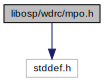
\includegraphics[width=177pt]{mpo_8h__incl}
\end{center}
\end{figure}
This graph shows which files directly or indirectly include this file\+:\nopagebreak
\begin{figure}[H]
\begin{center}
\leavevmode
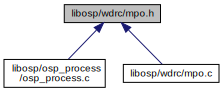
\includegraphics[width=296pt]{mpo_8h__dep__incl}
\end{center}
\end{figure}
\subsection*{Functions}
\begin{DoxyCompactItemize}
\item 
void \mbox{\hyperlink{mpo_8h_ae1fe3ef6535fbf9476ee597f411114c9}{mpo}} (float $\ast$input, float $\ast$pdB, float $\ast$wdrcdB, float mpo\+\_\+limit, size\+\_\+t len, float $\ast$out)
\begin{DoxyCompactList}\small\item\em Function to apply dynamic-\/range compression to a single sub-\/band of the output of the analysis filter bank. \end{DoxyCompactList}\end{DoxyCompactItemize}


\subsection{Function Documentation}
\mbox{\Hypertarget{mpo_8h_ae1fe3ef6535fbf9476ee597f411114c9}\label{mpo_8h_ae1fe3ef6535fbf9476ee597f411114c9}} 
\index{mpo.\+h@{mpo.\+h}!mpo@{mpo}}
\index{mpo@{mpo}!mpo.\+h@{mpo.\+h}}
\subsubsection{\texorpdfstring{mpo()}{mpo()}}
{\footnotesize\ttfamily void mpo (\begin{DoxyParamCaption}\item[{float $\ast$}]{input,  }\item[{float $\ast$}]{pdB,  }\item[{float $\ast$}]{wdrcdB,  }\item[{float}]{mpo\+\_\+limit,  }\item[{size\+\_\+t}]{len,  }\item[{float $\ast$}]{out }\end{DoxyParamCaption})}



Function to apply dynamic-\/range compression to a single sub-\/band of the output of the analysis filter bank. 

The peak detector output in dB S\+PL is needed as one of the inputs. The gain at 50 and 80 dB S\+PL is specified for the frequency sub-\/band, along with the lower and upper kneepoints in dB S\+PL. The compressor is linear below the lower kneepoint and applies compression limiting above the upper kneepoint


\begin{DoxyParams}{Parameters}
{\em input} & Pointer to the signal array at the frequency sub-\/band (output from sub-\/band filtering) \\
\hline
{\em pdB} & Pointer to the peak detector output array of the sub-\/band in dB S\+PL (output from peak\+\_\+to\+\_\+spl) \\
\hline
{\em wdrcdB} & Gain in dB at the sub-\/band frequency for an input at 50 dB S\+PL \\
\hline
{\em mpo\+\_\+limit} & Upper kneepoint in dB S\+PL for the sub-\/band \\
\hline
{\em len} & Length of the input array \\
\hline
{\em out} & Pointer to an array where the compressed output of the sub-\/band will be written. i.\+e. the output of M\+PO limiter \\
\hline
\end{DoxyParams}

\hypertarget{wdrc_8c}{}\section{libosp/wdrc/wdrc.c File Reference}
\label{wdrc_8c}\index{libosp/wdrc/wdrc.\+c@{libosp/wdrc/wdrc.\+c}}
{\ttfamily \#include \char`\"{}wdrc.\+h\char`\"{}}\newline
{\ttfamily \#include $<$math.\+h$>$}\newline
Include dependency graph for wdrc.\+c\+:\nopagebreak
\begin{figure}[H]
\begin{center}
\leavevmode
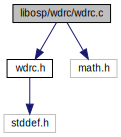
\includegraphics[width=193pt]{wdrc_8c__incl}
\end{center}
\end{figure}
\subsection*{Functions}
\begin{DoxyCompactItemize}
\item 
void \mbox{\hyperlink{wdrc_8c_a61466fe227a9fc80623fbee67f702d16}{wdrc}} (float $\ast$input, float $\ast$pdB, float gain50, float gain80, float knee\+\_\+low, float knee\+\_\+high, size\+\_\+t len, float $\ast$out)
\begin{DoxyCompactList}\small\item\em Function to apply dynamic-\/range compression to a single sub-\/band of the output of the analysis filter bank. \end{DoxyCompactList}\end{DoxyCompactItemize}


\subsection{Function Documentation}
\mbox{\Hypertarget{wdrc_8c_a61466fe227a9fc80623fbee67f702d16}\label{wdrc_8c_a61466fe227a9fc80623fbee67f702d16}} 
\index{wdrc.\+c@{wdrc.\+c}!wdrc@{wdrc}}
\index{wdrc@{wdrc}!wdrc.\+c@{wdrc.\+c}}
\subsubsection{\texorpdfstring{wdrc()}{wdrc()}}
{\footnotesize\ttfamily void wdrc (\begin{DoxyParamCaption}\item[{float $\ast$}]{input,  }\item[{float $\ast$}]{pdB,  }\item[{float}]{gain50,  }\item[{float}]{gain80,  }\item[{float}]{knee\+\_\+low,  }\item[{float}]{knee\+\_\+high,  }\item[{size\+\_\+t}]{len,  }\item[{float $\ast$}]{out }\end{DoxyParamCaption})}



Function to apply dynamic-\/range compression to a single sub-\/band of the output of the analysis filter bank. 

The peak detector output in dB S\+PL is needed as one of the inputs. The gain at 50 and 80 dB S\+PL is specified for the frequency sub-\/band, along with the lower and upper kneepoints in dB S\+PL. The compressor is linear below the lower kneepoint and applies compression limiting above the upper kneepoint


\begin{DoxyParams}{Parameters}
{\em input} & Pointer to the signal array at the frequency sub-\/band (output from sub-\/band filtering) \\
\hline
{\em pdB} & Pointer to the peak detector output array of the sub-\/band in dB S\+PL (output from peak\+\_\+to\+\_\+spl) \\
\hline
{\em gain50} & Gain in dB at the sub-\/band frequency for an input at 50 dB S\+PL \\
\hline
{\em gain80} & Gain in dB at the sub-\/band frequency for an input at 80 dB S\+PL \\
\hline
{\em knee\+\_\+low} & Lower kneepoint in dB S\+PL for the sub-\/band \\
\hline
{\em knee\+\_\+high} & Upper kneepoint in dB S\+PL for the sub-\/band \\
\hline
{\em len} & Length of the input array \\
\hline
{\em out} & Pointer to an array where the compressed output of the sub-\/band will be written. i.\+e. the output of W\+D\+RC \\
\hline
\end{DoxyParams}

\hypertarget{wdrc_8h}{}\section{libosp/wdrc/wdrc.h File Reference}
\label{wdrc_8h}\index{libosp/wdrc/wdrc.\+h@{libosp/wdrc/wdrc.\+h}}
{\ttfamily \#include $<$stddef.\+h$>$}\newline
Include dependency graph for wdrc.\+h\+:\nopagebreak
\begin{figure}[H]
\begin{center}
\leavevmode
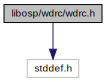
\includegraphics[width=178pt]{wdrc_8h__incl}
\end{center}
\end{figure}
This graph shows which files directly or indirectly include this file\+:\nopagebreak
\begin{figure}[H]
\begin{center}
\leavevmode
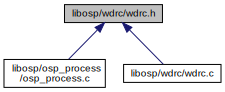
\includegraphics[width=298pt]{wdrc_8h__dep__incl}
\end{center}
\end{figure}
\subsection*{Functions}
\begin{DoxyCompactItemize}
\item 
void \mbox{\hyperlink{wdrc_8h_a61466fe227a9fc80623fbee67f702d16}{wdrc}} (float $\ast$input, float $\ast$pdB, float gain50, float gain80, float knee\+\_\+low, float knee\+\_\+high, size\+\_\+t len, float $\ast$out)
\begin{DoxyCompactList}\small\item\em Function to apply dynamic-\/range compression to a single sub-\/band of the output of the analysis filter bank. \end{DoxyCompactList}\end{DoxyCompactItemize}


\subsection{Function Documentation}
\mbox{\Hypertarget{wdrc_8h_a61466fe227a9fc80623fbee67f702d16}\label{wdrc_8h_a61466fe227a9fc80623fbee67f702d16}} 
\index{wdrc.\+h@{wdrc.\+h}!wdrc@{wdrc}}
\index{wdrc@{wdrc}!wdrc.\+h@{wdrc.\+h}}
\subsubsection{\texorpdfstring{wdrc()}{wdrc()}}
{\footnotesize\ttfamily void wdrc (\begin{DoxyParamCaption}\item[{float $\ast$}]{input,  }\item[{float $\ast$}]{pdB,  }\item[{float}]{gain50,  }\item[{float}]{gain80,  }\item[{float}]{knee\+\_\+low,  }\item[{float}]{knee\+\_\+high,  }\item[{size\+\_\+t}]{len,  }\item[{float $\ast$}]{out }\end{DoxyParamCaption})}



Function to apply dynamic-\/range compression to a single sub-\/band of the output of the analysis filter bank. 

The peak detector output in dB S\+PL is needed as one of the inputs. The gain at 50 and 80 dB S\+PL is specified for the frequency sub-\/band, along with the lower and upper kneepoints in dB S\+PL. The compressor is linear below the lower kneepoint and applies compression limiting above the upper kneepoint


\begin{DoxyParams}{Parameters}
{\em input} & Pointer to the signal array at the frequency sub-\/band (output from sub-\/band filtering) \\
\hline
{\em pdB} & Pointer to the peak detector output array of the sub-\/band in dB S\+PL (output from peak\+\_\+to\+\_\+spl) \\
\hline
{\em gain50} & Gain in dB at the sub-\/band frequency for an input at 50 dB S\+PL \\
\hline
{\em gain80} & Gain in dB at the sub-\/band frequency for an input at 80 dB S\+PL \\
\hline
{\em knee\+\_\+low} & Lower kneepoint in dB S\+PL for the sub-\/band \\
\hline
{\em knee\+\_\+high} & Upper kneepoint in dB S\+PL for the sub-\/band \\
\hline
{\em len} & Length of the input array \\
\hline
{\em out} & Pointer to an array where the compressed output of the sub-\/band will be written. i.\+e. the output of W\+D\+RC \\
\hline
\end{DoxyParams}

\hypertarget{wdrc__mpo__support_8c}{}\section{libosp/wdrc/wdrc\+\_\+mpo\+\_\+support.c File Reference}
\label{wdrc__mpo__support_8c}\index{libosp/wdrc/wdrc\+\_\+mpo\+\_\+support.\+c@{libosp/wdrc/wdrc\+\_\+mpo\+\_\+support.\+c}}
{\ttfamily \#include \char`\"{}wdrc\+\_\+mpo\+\_\+support.\+h\char`\"{}}\newline
Include dependency graph for wdrc\+\_\+mpo\+\_\+support.\+c\+:\nopagebreak
\begin{figure}[H]
\begin{center}
\leavevmode
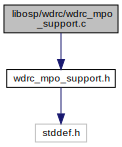
\includegraphics[width=195pt]{wdrc__mpo__support_8c__incl}
\end{center}
\end{figure}
\subsection*{Functions}
\begin{DoxyCompactItemize}
\item 
void \mbox{\hyperlink{wdrc__mpo__support_8c_aa9f96c6f6e22bbc863c8467195ff8dd9}{wdrc\+\_\+mpo\+\_\+support}} (float $\ast$pdB, float gain50, float gain80, float knee\+\_\+low, size\+\_\+t len, float $\ast$wdrcdB)
\begin{DoxyCompactList}\small\item\em Function to apply dynamic-\/range compression to a single sub-\/band of the output of the analysis filter bank. \end{DoxyCompactList}\end{DoxyCompactItemize}


\subsection{Function Documentation}
\mbox{\Hypertarget{wdrc__mpo__support_8c_aa9f96c6f6e22bbc863c8467195ff8dd9}\label{wdrc__mpo__support_8c_aa9f96c6f6e22bbc863c8467195ff8dd9}} 
\index{wdrc\+\_\+mpo\+\_\+support.\+c@{wdrc\+\_\+mpo\+\_\+support.\+c}!wdrc\+\_\+mpo\+\_\+support@{wdrc\+\_\+mpo\+\_\+support}}
\index{wdrc\+\_\+mpo\+\_\+support@{wdrc\+\_\+mpo\+\_\+support}!wdrc\+\_\+mpo\+\_\+support.\+c@{wdrc\+\_\+mpo\+\_\+support.\+c}}
\subsubsection{\texorpdfstring{wdrc\+\_\+mpo\+\_\+support()}{wdrc\_mpo\_support()}}
{\footnotesize\ttfamily void wdrc\+\_\+mpo\+\_\+support (\begin{DoxyParamCaption}\item[{float $\ast$}]{pdB,  }\item[{float}]{gain50,  }\item[{float}]{gain80,  }\item[{float}]{knee\+\_\+low,  }\item[{size\+\_\+t}]{len,  }\item[{float $\ast$}]{wdrcdB }\end{DoxyParamCaption})}



Function to apply dynamic-\/range compression to a single sub-\/band of the output of the analysis filter bank. 

The peak detector output in dB S\+PL is needed as one of the inputs. The gain at 50 and 80 dB S\+PL is specified for the frequency sub-\/band, along with the lower and upper kneepoints in dB S\+PL. The compressor is linear below the lower kneepoint and applies compression limiting above the upper kneepoint


\begin{DoxyParams}{Parameters}
{\em pdB} & Pointer to the peak detector output array of the sub-\/band in dB S\+PL (output from peak\+\_\+to\+\_\+spl) \\
\hline
{\em gain50} & Gain in dB at the sub-\/band frequency for an input at 50 dB S\+PL \\
\hline
{\em gain80} & Gain in dB at the sub-\/band frequency for an input at 80 dB S\+PL \\
\hline
{\em knee\+\_\+low} & Lower kneepoint in dB S\+PL for the sub-\/band \\
\hline
{\em len} & Length of the input array \\
\hline
{\em wdrcdB} & Pointer to an array where the compressed output of the sub-\/band will be written. i.\+e. the output of W\+D\+RC \\
\hline
\end{DoxyParams}

\hypertarget{wdrc__mpo__support_8h}{}\section{libosp/wdrc/wdrc\+\_\+mpo\+\_\+support.h File Reference}
\label{wdrc__mpo__support_8h}\index{libosp/wdrc/wdrc\+\_\+mpo\+\_\+support.\+h@{libosp/wdrc/wdrc\+\_\+mpo\+\_\+support.\+h}}
{\ttfamily \#include $<$stddef.\+h$>$}\newline
Include dependency graph for wdrc\+\_\+mpo\+\_\+support.\+h\+:\nopagebreak
\begin{figure}[H]
\begin{center}
\leavevmode
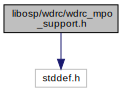
\includegraphics[width=195pt]{wdrc__mpo__support_8h__incl}
\end{center}
\end{figure}
This graph shows which files directly or indirectly include this file\+:\nopagebreak
\begin{figure}[H]
\begin{center}
\leavevmode
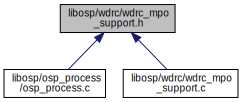
\includegraphics[width=314pt]{wdrc__mpo__support_8h__dep__incl}
\end{center}
\end{figure}
\subsection*{Functions}
\begin{DoxyCompactItemize}
\item 
void \mbox{\hyperlink{wdrc__mpo__support_8h_aa9f96c6f6e22bbc863c8467195ff8dd9}{wdrc\+\_\+mpo\+\_\+support}} (float $\ast$pdB, float gain50, float gain80, float knee\+\_\+low, size\+\_\+t len, float $\ast$wdrcdB)
\begin{DoxyCompactList}\small\item\em Function to apply dynamic-\/range compression to a single sub-\/band of the output of the analysis filter bank. \end{DoxyCompactList}\end{DoxyCompactItemize}


\subsection{Function Documentation}
\mbox{\Hypertarget{wdrc__mpo__support_8h_aa9f96c6f6e22bbc863c8467195ff8dd9}\label{wdrc__mpo__support_8h_aa9f96c6f6e22bbc863c8467195ff8dd9}} 
\index{wdrc\+\_\+mpo\+\_\+support.\+h@{wdrc\+\_\+mpo\+\_\+support.\+h}!wdrc\+\_\+mpo\+\_\+support@{wdrc\+\_\+mpo\+\_\+support}}
\index{wdrc\+\_\+mpo\+\_\+support@{wdrc\+\_\+mpo\+\_\+support}!wdrc\+\_\+mpo\+\_\+support.\+h@{wdrc\+\_\+mpo\+\_\+support.\+h}}
\subsubsection{\texorpdfstring{wdrc\+\_\+mpo\+\_\+support()}{wdrc\_mpo\_support()}}
{\footnotesize\ttfamily void wdrc\+\_\+mpo\+\_\+support (\begin{DoxyParamCaption}\item[{float $\ast$}]{pdB,  }\item[{float}]{gain50,  }\item[{float}]{gain80,  }\item[{float}]{knee\+\_\+low,  }\item[{size\+\_\+t}]{len,  }\item[{float $\ast$}]{wdrcdB }\end{DoxyParamCaption})}



Function to apply dynamic-\/range compression to a single sub-\/band of the output of the analysis filter bank. 

The peak detector output in dB S\+PL is needed as one of the inputs. The gain at 50 and 80 dB S\+PL is specified for the frequency sub-\/band, along with the lower and upper kneepoints in dB S\+PL. The compressor is linear below the lower kneepoint and applies compression limiting above the upper kneepoint


\begin{DoxyParams}{Parameters}
{\em pdB} & Pointer to the peak detector output array of the sub-\/band in dB S\+PL (output from peak\+\_\+to\+\_\+spl) \\
\hline
{\em gain50} & Gain in dB at the sub-\/band frequency for an input at 50 dB S\+PL \\
\hline
{\em gain80} & Gain in dB at the sub-\/band frequency for an input at 80 dB S\+PL \\
\hline
{\em knee\+\_\+low} & Lower kneepoint in dB S\+PL for the sub-\/band \\
\hline
{\em len} & Length of the input array \\
\hline
{\em wdrcdB} & Pointer to an array where the compressed output of the sub-\/band will be written. i.\+e. the output of W\+D\+RC \\
\hline
\end{DoxyParams}

\hypertarget{logger_8c}{}\section{osp/logger.c File Reference}
\label{logger_8c}\index{osp/logger.\+c@{osp/logger.\+c}}
{\ttfamily \#include $<$sys/types.\+h$>$}\newline
{\ttfamily \#include $<$sys/stat.\+h$>$}\newline
{\ttfamily \#include $<$stdio.\+h$>$}\newline
{\ttfamily \#include $<$time.\+h$>$}\newline
{\ttfamily \#include $<$stdlib.\+h$>$}\newline
{\ttfamily \#include \char`\"{}constants.\+h\char`\"{}}\newline
{\ttfamily \#include $<$unistd.\+h$>$}\newline
Include dependency graph for logger.\+c\+:\nopagebreak
\begin{figure}[H]
\begin{center}
\leavevmode
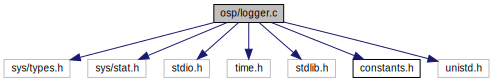
\includegraphics[width=350pt]{logger_8c__incl}
\end{center}
\end{figure}
\subsection*{Functions}
\begin{DoxyCompactItemize}
\item 
F\+I\+LE $\ast$ \mbox{\hyperlink{logger_8c_abc755fd3e95478e2f070e3fe82d79f32}{file\+\_\+logger\+\_\+init}} (char $\ast$filename)
\item 
int \mbox{\hyperlink{logger_8c_a88f4e5965b505769093e24e75e32810e}{file\+\_\+logger\+\_\+log\+\_\+osp\+\_\+data}} (F\+I\+LE $\ast$fd, \mbox{\hyperlink{constants_8h_a2d1d78531fe12807c3852488556d5a4b}{osp\+\_\+user\+\_\+data}} $\ast$data)
\item 
void \mbox{\hyperlink{logger_8c_ad6e74a19c96a498d85c61c7d2ca74366}{file\+\_\+logger\+\_\+log\+\_\+message}} (F\+I\+LE $\ast$fd, char $\ast$message)
\item 
void \mbox{\hyperlink{logger_8c_a3ef5788057d6e3129d6fe83183e2475b}{file\+\_\+logger\+\_\+close}} (F\+I\+LE $\ast$fd)
\end{DoxyCompactItemize}


\subsection{Function Documentation}
\mbox{\Hypertarget{logger_8c_a3ef5788057d6e3129d6fe83183e2475b}\label{logger_8c_a3ef5788057d6e3129d6fe83183e2475b}} 
\index{logger.\+c@{logger.\+c}!file\+\_\+logger\+\_\+close@{file\+\_\+logger\+\_\+close}}
\index{file\+\_\+logger\+\_\+close@{file\+\_\+logger\+\_\+close}!logger.\+c@{logger.\+c}}
\subsubsection{\texorpdfstring{file\+\_\+logger\+\_\+close()}{file\_logger\_close()}}
{\footnotesize\ttfamily void file\+\_\+logger\+\_\+close (\begin{DoxyParamCaption}\item[{F\+I\+LE $\ast$}]{fd }\end{DoxyParamCaption})}

\mbox{\Hypertarget{logger_8c_abc755fd3e95478e2f070e3fe82d79f32}\label{logger_8c_abc755fd3e95478e2f070e3fe82d79f32}} 
\index{logger.\+c@{logger.\+c}!file\+\_\+logger\+\_\+init@{file\+\_\+logger\+\_\+init}}
\index{file\+\_\+logger\+\_\+init@{file\+\_\+logger\+\_\+init}!logger.\+c@{logger.\+c}}
\subsubsection{\texorpdfstring{file\+\_\+logger\+\_\+init()}{file\_logger\_init()}}
{\footnotesize\ttfamily F\+I\+LE$\ast$ file\+\_\+logger\+\_\+init (\begin{DoxyParamCaption}\item[{char $\ast$}]{filename }\end{DoxyParamCaption})}

\mbox{\Hypertarget{logger_8c_ad6e74a19c96a498d85c61c7d2ca74366}\label{logger_8c_ad6e74a19c96a498d85c61c7d2ca74366}} 
\index{logger.\+c@{logger.\+c}!file\+\_\+logger\+\_\+log\+\_\+message@{file\+\_\+logger\+\_\+log\+\_\+message}}
\index{file\+\_\+logger\+\_\+log\+\_\+message@{file\+\_\+logger\+\_\+log\+\_\+message}!logger.\+c@{logger.\+c}}
\subsubsection{\texorpdfstring{file\+\_\+logger\+\_\+log\+\_\+message()}{file\_logger\_log\_message()}}
{\footnotesize\ttfamily void file\+\_\+logger\+\_\+log\+\_\+message (\begin{DoxyParamCaption}\item[{F\+I\+LE $\ast$}]{fd,  }\item[{char $\ast$}]{message }\end{DoxyParamCaption})}

\mbox{\Hypertarget{logger_8c_a88f4e5965b505769093e24e75e32810e}\label{logger_8c_a88f4e5965b505769093e24e75e32810e}} 
\index{logger.\+c@{logger.\+c}!file\+\_\+logger\+\_\+log\+\_\+osp\+\_\+data@{file\+\_\+logger\+\_\+log\+\_\+osp\+\_\+data}}
\index{file\+\_\+logger\+\_\+log\+\_\+osp\+\_\+data@{file\+\_\+logger\+\_\+log\+\_\+osp\+\_\+data}!logger.\+c@{logger.\+c}}
\subsubsection{\texorpdfstring{file\+\_\+logger\+\_\+log\+\_\+osp\+\_\+data()}{file\_logger\_log\_osp\_data()}}
{\footnotesize\ttfamily int file\+\_\+logger\+\_\+log\+\_\+osp\+\_\+data (\begin{DoxyParamCaption}\item[{F\+I\+LE $\ast$}]{fd,  }\item[{\mbox{\hyperlink{constants_8h_a2d1d78531fe12807c3852488556d5a4b}{osp\+\_\+user\+\_\+data}} $\ast$}]{data }\end{DoxyParamCaption})}


\hypertarget{osp_2logger_8h}{}\section{osp/logger.h File Reference}
\label{osp_2logger_8h}\index{osp/logger.\+h@{osp/logger.\+h}}
This graph shows which files directly or indirectly include this file\+:\nopagebreak
\begin{figure}[H]
\begin{center}
\leavevmode
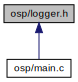
\includegraphics[width=150pt]{osp_2logger_8h__dep__incl}
\end{center}
\end{figure}
\subsection*{Functions}
\begin{DoxyCompactItemize}
\item 
F\+I\+LE $\ast$ \mbox{\hyperlink{osp_2logger_8h_a3520372b67c25934aa63d9a064e382c6}{file\+\_\+logger\+\_\+init}} (const char $\ast$filename)
\item 
int \mbox{\hyperlink{osp_2logger_8h_a88f4e5965b505769093e24e75e32810e}{file\+\_\+logger\+\_\+log\+\_\+osp\+\_\+data}} (F\+I\+LE $\ast$fd, \mbox{\hyperlink{constants_8h_a2d1d78531fe12807c3852488556d5a4b}{osp\+\_\+user\+\_\+data}} $\ast$data)
\item 
int \mbox{\hyperlink{osp_2logger_8h_af70ab074b22a07e777e7e7b0443a1def}{file\+\_\+logger\+\_\+log\+\_\+message}} (F\+I\+LE $\ast$fd, char $\ast$message)
\item 
void \mbox{\hyperlink{osp_2logger_8h_a3ef5788057d6e3129d6fe83183e2475b}{file\+\_\+logger\+\_\+close}} (F\+I\+LE $\ast$fd)
\end{DoxyCompactItemize}


\subsection{Function Documentation}
\mbox{\Hypertarget{osp_2logger_8h_a3ef5788057d6e3129d6fe83183e2475b}\label{osp_2logger_8h_a3ef5788057d6e3129d6fe83183e2475b}} 
\index{osp/logger.\+h@{osp/logger.\+h}!file\+\_\+logger\+\_\+close@{file\+\_\+logger\+\_\+close}}
\index{file\+\_\+logger\+\_\+close@{file\+\_\+logger\+\_\+close}!osp/logger.\+h@{osp/logger.\+h}}
\subsubsection{\texorpdfstring{file\+\_\+logger\+\_\+close()}{file\_logger\_close()}}
{\footnotesize\ttfamily void file\+\_\+logger\+\_\+close (\begin{DoxyParamCaption}\item[{F\+I\+LE $\ast$}]{fd }\end{DoxyParamCaption})}

\mbox{\Hypertarget{osp_2logger_8h_a3520372b67c25934aa63d9a064e382c6}\label{osp_2logger_8h_a3520372b67c25934aa63d9a064e382c6}} 
\index{osp/logger.\+h@{osp/logger.\+h}!file\+\_\+logger\+\_\+init@{file\+\_\+logger\+\_\+init}}
\index{file\+\_\+logger\+\_\+init@{file\+\_\+logger\+\_\+init}!osp/logger.\+h@{osp/logger.\+h}}
\subsubsection{\texorpdfstring{file\+\_\+logger\+\_\+init()}{file\_logger\_init()}}
{\footnotesize\ttfamily F\+I\+LE$\ast$ file\+\_\+logger\+\_\+init (\begin{DoxyParamCaption}\item[{const char $\ast$}]{filename }\end{DoxyParamCaption})}

\mbox{\Hypertarget{osp_2logger_8h_af70ab074b22a07e777e7e7b0443a1def}\label{osp_2logger_8h_af70ab074b22a07e777e7e7b0443a1def}} 
\index{osp/logger.\+h@{osp/logger.\+h}!file\+\_\+logger\+\_\+log\+\_\+message@{file\+\_\+logger\+\_\+log\+\_\+message}}
\index{file\+\_\+logger\+\_\+log\+\_\+message@{file\+\_\+logger\+\_\+log\+\_\+message}!osp/logger.\+h@{osp/logger.\+h}}
\subsubsection{\texorpdfstring{file\+\_\+logger\+\_\+log\+\_\+message()}{file\_logger\_log\_message()}}
{\footnotesize\ttfamily int file\+\_\+logger\+\_\+log\+\_\+message (\begin{DoxyParamCaption}\item[{F\+I\+LE $\ast$}]{fd,  }\item[{char $\ast$}]{message }\end{DoxyParamCaption})}

\mbox{\Hypertarget{osp_2logger_8h_a88f4e5965b505769093e24e75e32810e}\label{osp_2logger_8h_a88f4e5965b505769093e24e75e32810e}} 
\index{osp/logger.\+h@{osp/logger.\+h}!file\+\_\+logger\+\_\+log\+\_\+osp\+\_\+data@{file\+\_\+logger\+\_\+log\+\_\+osp\+\_\+data}}
\index{file\+\_\+logger\+\_\+log\+\_\+osp\+\_\+data@{file\+\_\+logger\+\_\+log\+\_\+osp\+\_\+data}!osp/logger.\+h@{osp/logger.\+h}}
\subsubsection{\texorpdfstring{file\+\_\+logger\+\_\+log\+\_\+osp\+\_\+data()}{file\_logger\_log\_osp\_data()}}
{\footnotesize\ttfamily int file\+\_\+logger\+\_\+log\+\_\+osp\+\_\+data (\begin{DoxyParamCaption}\item[{F\+I\+LE $\ast$}]{fd,  }\item[{\mbox{\hyperlink{constants_8h_a2d1d78531fe12807c3852488556d5a4b}{osp\+\_\+user\+\_\+data}} $\ast$}]{data }\end{DoxyParamCaption})}


\hypertarget{libosp_2osp__process_2logger_8h}{}\section{libosp/osp\+\_\+process/logger.h File Reference}
\label{libosp_2osp__process_2logger_8h}\index{libosp/osp\+\_\+process/logger.\+h@{libosp/osp\+\_\+process/logger.\+h}}
{\ttfamily \#include $<$stdio.\+h$>$}\newline
{\ttfamily \#include $<$stdlib.\+h$>$}\newline
Include dependency graph for logger.\+h\+:\nopagebreak
\begin{figure}[H]
\begin{center}
\leavevmode
\includegraphics[width=192pt]{libosp_2osp__process_2logger_8h__incl}
\end{center}
\end{figure}
This graph shows which files directly or indirectly include this file\+:\nopagebreak
\begin{figure}[H]
\begin{center}
\leavevmode
\includegraphics[width=182pt]{libosp_2osp__process_2logger_8h__dep__incl}
\end{center}
\end{figure}
\subsection*{Macros}
\begin{DoxyCompactItemize}
\item 
\#define \mbox{\hyperlink{libosp_2osp__process_2logger_8h_a04ed3ac2f178cdcd0333c005a2923958}{M\+A\+X\+\_\+\+W\+R\+I\+T\+E\+\_\+\+L\+EN}}~200
\item 
\#define \mbox{\hyperlink{libosp_2osp__process_2logger_8h_a2d6d232d4b73a9001954d9344e7dc6cc}{\+\_\+\+T\+I\+\_\+\+D\+SP}}
\item 
\#define \mbox{\hyperlink{libosp_2osp__process_2logger_8h_ab9cc7514357ca48166849172842cd1fc}{\+\_\+\+P\+R\+I\+NT}}(fmt,  args...)
\item 
\#define \mbox{\hyperlink{libosp_2osp__process_2logger_8h_aaf2698d28214fc0f1d3c13efcfe62906}{D\+BG}}(fmg,  args...)
\item 
\#define \mbox{\hyperlink{libosp_2osp__process_2logger_8h_aed1edcc4c4106ded407551794cd9d81d}{D\+B\+G\+D\+A\+TA}}(data,  len)
\item 
\#define \mbox{\hyperlink{libosp_2osp__process_2logger_8h_a757e7ca1cb8d8c32eb898c929ae48ca0}{A\+S\+S\+E\+RT}}(cond,  fmt,  args...)
\item 
\#define \mbox{\hyperlink{libosp_2osp__process_2logger_8h_a77837c49da9b8b5b86bc5a0d11702b21}{I\+N\+FO}}(fmt,  args...)~\mbox{\hyperlink{libosp_2osp__process_2logger_8h_ab9cc7514357ca48166849172842cd1fc}{\+\_\+\+P\+R\+I\+NT}}(\char`\"{}\mbox{[}info\mbox{]} \%s() \char`\"{} fmt, \+\_\+\+\_\+\+F\+U\+N\+C\+T\+I\+O\+N\+\_\+\+\_\+, \#\#args);
\item 
\#define \mbox{\hyperlink{libosp_2osp__process_2logger_8h_aa9b914884d7e4c95be9e9cb2b99d385b}{E\+R\+R\+OR}}(fmt,  args...)~\mbox{\hyperlink{libosp_2osp__process_2logger_8h_ab9cc7514357ca48166849172842cd1fc}{\+\_\+\+P\+R\+I\+NT}}(\char`\"{}\mbox{[}error\mbox{]} \%s() \char`\"{} fmt, \+\_\+\+\_\+\+F\+U\+N\+C\+T\+I\+O\+N\+\_\+\+\_\+, \#\#args);
\end{DoxyCompactItemize}


\subsection{Macro Definition Documentation}
\mbox{\Hypertarget{libosp_2osp__process_2logger_8h_ab9cc7514357ca48166849172842cd1fc}\label{libosp_2osp__process_2logger_8h_ab9cc7514357ca48166849172842cd1fc}} 
\index{libosp/osp\+\_\+process/logger.\+h@{libosp/osp\+\_\+process/logger.\+h}!\+\_\+\+P\+R\+I\+NT@{\+\_\+\+P\+R\+I\+NT}}
\index{\+\_\+\+P\+R\+I\+NT@{\+\_\+\+P\+R\+I\+NT}!libosp/osp\+\_\+process/logger.\+h@{libosp/osp\+\_\+process/logger.\+h}}
\subsubsection{\texorpdfstring{\+\_\+\+P\+R\+I\+NT}{\_PRINT}}
{\footnotesize\ttfamily \#define \+\_\+\+P\+R\+I\+NT(\begin{DoxyParamCaption}\item[{}]{fmt,  }\item[{}]{args... }\end{DoxyParamCaption})}

{\bfseries Value\+:}
\begin{DoxyCode}
\textcolor{keywordflow}{do} \{ \(\backslash\)
    \} \textcolor{keywordflow}{while} (0)
\end{DoxyCode}
\mbox{\Hypertarget{libosp_2osp__process_2logger_8h_a2d6d232d4b73a9001954d9344e7dc6cc}\label{libosp_2osp__process_2logger_8h_a2d6d232d4b73a9001954d9344e7dc6cc}} 
\index{libosp/osp\+\_\+process/logger.\+h@{libosp/osp\+\_\+process/logger.\+h}!\+\_\+\+T\+I\+\_\+\+D\+SP@{\+\_\+\+T\+I\+\_\+\+D\+SP}}
\index{\+\_\+\+T\+I\+\_\+\+D\+SP@{\+\_\+\+T\+I\+\_\+\+D\+SP}!libosp/osp\+\_\+process/logger.\+h@{libosp/osp\+\_\+process/logger.\+h}}
\subsubsection{\texorpdfstring{\+\_\+\+T\+I\+\_\+\+D\+SP}{\_TI\_DSP}}
{\footnotesize\ttfamily \#define \+\_\+\+T\+I\+\_\+\+D\+SP}

\mbox{\Hypertarget{libosp_2osp__process_2logger_8h_a757e7ca1cb8d8c32eb898c929ae48ca0}\label{libosp_2osp__process_2logger_8h_a757e7ca1cb8d8c32eb898c929ae48ca0}} 
\index{libosp/osp\+\_\+process/logger.\+h@{libosp/osp\+\_\+process/logger.\+h}!A\+S\+S\+E\+RT@{A\+S\+S\+E\+RT}}
\index{A\+S\+S\+E\+RT@{A\+S\+S\+E\+RT}!libosp/osp\+\_\+process/logger.\+h@{libosp/osp\+\_\+process/logger.\+h}}
\subsubsection{\texorpdfstring{A\+S\+S\+E\+RT}{ASSERT}}
{\footnotesize\ttfamily \#define A\+S\+S\+E\+RT(\begin{DoxyParamCaption}\item[{}]{cond,  }\item[{}]{fmt,  }\item[{}]{args... }\end{DoxyParamCaption})}

{\bfseries Value\+:}
\begin{DoxyCode}
\textcolor{keywordflow}{do} \{                    \(\backslash\)
    if (!(cond)) \{                          \(\backslash\)
        \_PRINT(\textcolor{stringliteral}{"[assert] %s() "} fmt, \_\_FUNCTION\_\_, ##args); \(\backslash\)
        exit(1);                        \(\backslash\)
    \}                               \(\backslash\)
\} \textcolor{keywordflow}{while}(0)
\end{DoxyCode}
\mbox{\Hypertarget{libosp_2osp__process_2logger_8h_aaf2698d28214fc0f1d3c13efcfe62906}\label{libosp_2osp__process_2logger_8h_aaf2698d28214fc0f1d3c13efcfe62906}} 
\index{libosp/osp\+\_\+process/logger.\+h@{libosp/osp\+\_\+process/logger.\+h}!D\+BG@{D\+BG}}
\index{D\+BG@{D\+BG}!libosp/osp\+\_\+process/logger.\+h@{libosp/osp\+\_\+process/logger.\+h}}
\subsubsection{\texorpdfstring{D\+BG}{DBG}}
{\footnotesize\ttfamily \#define D\+BG(\begin{DoxyParamCaption}\item[{}]{fmg,  }\item[{}]{args... }\end{DoxyParamCaption})}

\mbox{\Hypertarget{libosp_2osp__process_2logger_8h_aed1edcc4c4106ded407551794cd9d81d}\label{libosp_2osp__process_2logger_8h_aed1edcc4c4106ded407551794cd9d81d}} 
\index{libosp/osp\+\_\+process/logger.\+h@{libosp/osp\+\_\+process/logger.\+h}!D\+B\+G\+D\+A\+TA@{D\+B\+G\+D\+A\+TA}}
\index{D\+B\+G\+D\+A\+TA@{D\+B\+G\+D\+A\+TA}!libosp/osp\+\_\+process/logger.\+h@{libosp/osp\+\_\+process/logger.\+h}}
\subsubsection{\texorpdfstring{D\+B\+G\+D\+A\+TA}{DBGDATA}}
{\footnotesize\ttfamily \#define D\+B\+G\+D\+A\+TA(\begin{DoxyParamCaption}\item[{}]{data,  }\item[{}]{len }\end{DoxyParamCaption})}

\mbox{\Hypertarget{libosp_2osp__process_2logger_8h_aa9b914884d7e4c95be9e9cb2b99d385b}\label{libosp_2osp__process_2logger_8h_aa9b914884d7e4c95be9e9cb2b99d385b}} 
\index{libosp/osp\+\_\+process/logger.\+h@{libosp/osp\+\_\+process/logger.\+h}!E\+R\+R\+OR@{E\+R\+R\+OR}}
\index{E\+R\+R\+OR@{E\+R\+R\+OR}!libosp/osp\+\_\+process/logger.\+h@{libosp/osp\+\_\+process/logger.\+h}}
\subsubsection{\texorpdfstring{E\+R\+R\+OR}{ERROR}}
{\footnotesize\ttfamily \#define E\+R\+R\+OR(\begin{DoxyParamCaption}\item[{}]{fmt,  }\item[{}]{args... }\end{DoxyParamCaption})~\mbox{\hyperlink{libosp_2osp__process_2logger_8h_ab9cc7514357ca48166849172842cd1fc}{\+\_\+\+P\+R\+I\+NT}}(\char`\"{}\mbox{[}error\mbox{]} \%s() \char`\"{} fmt, \+\_\+\+\_\+\+F\+U\+N\+C\+T\+I\+O\+N\+\_\+\+\_\+, \#\#args);}

\mbox{\Hypertarget{libosp_2osp__process_2logger_8h_a77837c49da9b8b5b86bc5a0d11702b21}\label{libosp_2osp__process_2logger_8h_a77837c49da9b8b5b86bc5a0d11702b21}} 
\index{libosp/osp\+\_\+process/logger.\+h@{libosp/osp\+\_\+process/logger.\+h}!I\+N\+FO@{I\+N\+FO}}
\index{I\+N\+FO@{I\+N\+FO}!libosp/osp\+\_\+process/logger.\+h@{libosp/osp\+\_\+process/logger.\+h}}
\subsubsection{\texorpdfstring{I\+N\+FO}{INFO}}
{\footnotesize\ttfamily \#define I\+N\+FO(\begin{DoxyParamCaption}\item[{}]{fmt,  }\item[{}]{args... }\end{DoxyParamCaption})~\mbox{\hyperlink{libosp_2osp__process_2logger_8h_ab9cc7514357ca48166849172842cd1fc}{\+\_\+\+P\+R\+I\+NT}}(\char`\"{}\mbox{[}info\mbox{]} \%s() \char`\"{} fmt, \+\_\+\+\_\+\+F\+U\+N\+C\+T\+I\+O\+N\+\_\+\+\_\+, \#\#args);}

\mbox{\Hypertarget{libosp_2osp__process_2logger_8h_a04ed3ac2f178cdcd0333c005a2923958}\label{libosp_2osp__process_2logger_8h_a04ed3ac2f178cdcd0333c005a2923958}} 
\index{libosp/osp\+\_\+process/logger.\+h@{libosp/osp\+\_\+process/logger.\+h}!M\+A\+X\+\_\+\+W\+R\+I\+T\+E\+\_\+\+L\+EN@{M\+A\+X\+\_\+\+W\+R\+I\+T\+E\+\_\+\+L\+EN}}
\index{M\+A\+X\+\_\+\+W\+R\+I\+T\+E\+\_\+\+L\+EN@{M\+A\+X\+\_\+\+W\+R\+I\+T\+E\+\_\+\+L\+EN}!libosp/osp\+\_\+process/logger.\+h@{libosp/osp\+\_\+process/logger.\+h}}
\subsubsection{\texorpdfstring{M\+A\+X\+\_\+\+W\+R\+I\+T\+E\+\_\+\+L\+EN}{MAX\_WRITE\_LEN}}
{\footnotesize\ttfamily \#define M\+A\+X\+\_\+\+W\+R\+I\+T\+E\+\_\+\+L\+EN~200}


\hypertarget{main_8c}{}\section{osp/main.c File Reference}
\label{main_8c}\index{osp/main.\+c@{osp/main.\+c}}
{\ttfamily \#include $<$stdio.\+h$>$}\newline
{\ttfamily \#include $<$string.\+h$>$}\newline
{\ttfamily \#include $<$signal.\+h$>$}\newline
{\ttfamily \#include $<$stdlib.\+h$>$}\newline
{\ttfamily \#include $<$unistd.\+h$>$}\newline
{\ttfamily \#include $<$limits.\+h$>$}\newline
{\ttfamily \#include $<$execinfo.\+h$>$}\newline
{\ttfamily \#include $<$math.\+h$>$}\newline
{\ttfamily \#include $<$pthread.\+h$>$}\newline
{\ttfamily \#include $<$errno.\+h$>$}\newline
{\ttfamily \#include $<$sys/types.\+h$>$}\newline
{\ttfamily \#include $<$ifaddrs.\+h$>$}\newline
{\ttfamily \#include $<$sys/socket.\+h$>$}\newline
{\ttfamily \#include $<$arpa/inet.\+h$>$}\newline
{\ttfamily \#include $<$netinet/in.\+h$>$}\newline
{\ttfamily \#include \char`\"{}osp\+\_\+tcp.\+h\char`\"{}}\newline
{\ttfamily \#include \char`\"{}osp\+\_\+process.\+h\char`\"{}}\newline
{\ttfamily \#include \char`\"{}resample.\+h\char`\"{}}\newline
{\ttfamily \#include \char`\"{}utilities.\+h\char`\"{}}\newline
{\ttfamily \#include \char`\"{}port\+\_\+wrapper.\+h\char`\"{}}\newline
{\ttfamily \#include \char`\"{}constants.\+h\char`\"{}}\newline
{\ttfamily \#include \char`\"{}logger.\+h\char`\"{}}\newline
{\ttfamily \#include \char`\"{}jsmn.\+h\char`\"{}}\newline
Include dependency graph for main.\+c\+:\nopagebreak
\begin{figure}[H]
\begin{center}
\leavevmode
\includegraphics[width=350pt]{main_8c__incl}
\end{center}
\end{figure}
\subsection*{Macros}
\begin{DoxyCompactItemize}
\item 
\#define \mbox{\hyperlink{main_8c_a123836f658bbae1fe968e88c71d9f59f}{U\+I\+\_\+\+P\+O\+RT}}~8001
\item 
\#define \mbox{\hyperlink{main_8c_a4b76a0c2859cfd819a343a780070ee2b}{S\+A\+M\+P\+L\+E\+\_\+\+R\+A\+TE}}~96000
\item 
\#define \mbox{\hyperlink{main_8c_af4f62216aa14e0407faa6631e9ec4c62}{F\+R\+A\+M\+E\+S\+\_\+\+P\+E\+R\+\_\+\+B\+U\+F\+F\+ER}}~96
\item 
\#define \mbox{\hyperlink{main_8c_ac82612e6326e939ae27e62ce1be9c8eb}{D\+\_\+\+A\+T\+T\+E\+N\+U\+A\+T\+I\+O\+N\+\_\+\+F\+A\+C\+T\+OR}}~(0.\+025)
\item 
\#define \mbox{\hyperlink{main_8c_a6242a25f9d996f0cc4f4cdb911218b75}{A\+R\+R\+A\+Y\+\_\+\+S\+I\+ZE}}(x)~(sizeof((x)) / sizeof((x)\mbox{[}0\mbox{]}))
\item 
\#define \mbox{\hyperlink{main_8c_a91fea349332c05eb78ce3c17202e1dc9}{O\+P\+T\+\_\+\+S\+T\+R\+I\+NG}}~\char`\"{}Enter \textbackslash{}\char`\"{}a\textbackslash{}\char`\"{} to enable hearing aid algorithm, \textbackslash{}\char`\"{}d\textbackslash{}\char`\"{} to disable \textbackslash{}\char`\"{}q\textbackslash{}\char`\"{} to quit\textbackslash{}n\char`\"{}
\end{DoxyCompactItemize}
\subsection*{Functions}
\begin{DoxyCompactItemize}
\item 
static float \mbox{\hyperlink{main_8c_ab352b1ff7a758e40b3072874726eba4c}{log2lin}} (float db)
\item 
static void \mbox{\hyperlink{main_8c_a64a6014565bb3e03294ec4a952d5add0}{usage}} ()
\item 
static void $\ast$ \mbox{\hyperlink{main_8c_a5eb5b7c33ec3a1b84b4dc75b6bc20dfd}{announce\+\_\+presence}} (void $\ast$tid)
\item 
static void \mbox{\hyperlink{main_8c_abbb0d46c0f00de5ea4ce0c647ceac666}{run\+\_\+loopback}} (\mbox{\hyperlink{constants_8h_a2d1d78531fe12807c3852488556d5a4b}{osp\+\_\+user\+\_\+data}} $\ast$osp\+\_\+data, float $\ast$inL, float $\ast$inR, float $\ast$outL, float $\ast$outR, size\+\_\+t len)
\item 
static int \mbox{\hyperlink{main_8c_a4bed96c09ac6c23015dab100e83a3996}{file\+\_\+loopback\+\_\+init}} (\mbox{\hyperlink{port__wrapper_8h_a44712da21c339df7c0735d4bab71a303}{file\+\_\+loopback\+\_\+context}} $\ast$ctx, const char $\ast$in\+\_\+file, const char $\ast$out\+\_\+file)
\item 
static void \mbox{\hyperlink{main_8c_a797c8fa6667f63d3cac9f1d378bb6851}{file\+\_\+loopback\+\_\+close}} (\mbox{\hyperlink{port__wrapper_8h_a44712da21c339df7c0735d4bab71a303}{file\+\_\+loopback\+\_\+context}} $\ast$ctx)
\item 
static int \mbox{\hyperlink{main_8c_a2ca50a57ce898682d8042211eee429e2}{file\+\_\+context\+\_\+write}} (\mbox{\hyperlink{port__wrapper_8h_a44712da21c339df7c0735d4bab71a303}{file\+\_\+loopback\+\_\+context}} $\ast$file\+\_\+ctx)
\item 
static int \mbox{\hyperlink{main_8c_aba4b29cdd5da8c4196dcc895431f6436}{file\+\_\+loopback\+\_\+run}} (const char $\ast$in\+\_\+file, const char $\ast$out\+\_\+file, unsigned int frames\+\_\+per\+\_\+buffer)
\item 
static int \mbox{\hyperlink{main_8c_ab8a38f850fea34a115fda3140af8b774}{run\+\_\+pa\+\_\+loopback}} (unsigned int sample\+\_\+rate, unsigned int frames\+\_\+per\+\_\+buffer, const char $\ast$in\+\_\+file, const char $\ast$out\+\_\+file, \mbox{\hyperlink{constants_8h_a2d1d78531fe12807c3852488556d5a4b}{osp\+\_\+user\+\_\+data}} $\ast$osp\+\_\+data)
\item 
static void \mbox{\hyperlink{main_8c_a4db999af4611cf4620ccec2ebf6e6a0d}{run\+\_\+loopback\+\_\+null}} (unsigned long count, unsigned int frames\+\_\+per\+\_\+buffer)
\item 
static int \mbox{\hyperlink{main_8c_a86ff0d7ff30269dba677b358fcabc387}{init\+\_\+pa}} (\mbox{\hyperlink{constants_8h_aba6e2261d5c6ef36dedb5b45ba0fc4ae}{pa\+\_\+user\+\_\+data}} $\ast$pa\+\_\+data, unsigned int samp\+\_\+rate, unsigned int frames\+\_\+per\+\_\+buffer)
\item 
static int \mbox{\hyperlink{main_8c_aa34be8cf0278cb357c2c5960f4c557c6}{close\+\_\+pa}} ()
\item 
static int \mbox{\hyperlink{main_8c_a1eb914c7767ba47fd3463871577c3662}{run\+\_\+pa\+\_\+key}} (\mbox{\hyperlink{constants_8h_a2d1d78531fe12807c3852488556d5a4b}{osp\+\_\+user\+\_\+data}} $\ast$osp\+\_\+data, unsigned int samp\+\_\+rate, unsigned int frames\+\_\+per\+\_\+buffer, float attenuation\+\_\+factor)
\item 
static int \mbox{\hyperlink{main_8c_a5c1a351ba62dfc0d60b39c5382c38636}{run\+\_\+pa\+\_\+tcp}} (\mbox{\hyperlink{constants_8h_a2d1d78531fe12807c3852488556d5a4b}{osp\+\_\+user\+\_\+data}} $\ast$osp\+\_\+data, unsigned int samp\+\_\+rate, unsigned int frames\+\_\+per\+\_\+buffer, float attenuation\+\_\+factor)
\item 
static int \mbox{\hyperlink{main_8c_ab474a7b7ec06d48e6d807ac2c063cc96}{playback\+\_\+file}} (\mbox{\hyperlink{constants_8h_a2d1d78531fe12807c3852488556d5a4b}{osp\+\_\+user\+\_\+data}} $\ast$osp\+\_\+data, unsigned int samp\+\_\+rate, unsigned int frames\+\_\+per\+\_\+buffer, float attenuation\+\_\+factor)
\item 
static int \mbox{\hyperlink{main_8c_a270935c92a12999bc75deb0ec045a4cd}{run\+\_\+pa\+\_\+tcp\+\_\+4afc}} (\mbox{\hyperlink{constants_8h_a2d1d78531fe12807c3852488556d5a4b}{osp\+\_\+user\+\_\+data}} $\ast$osp\+\_\+data, unsigned int samp\+\_\+rate, unsigned int frames\+\_\+per\+\_\+buffer, float attenuation\+\_\+factor)
\item 
int \mbox{\hyperlink{main_8c_a3c04138a5bfe5d72780bb7e82a18e627}{main}} (int argc, char $\ast$$\ast$argv)
\end{DoxyCompactItemize}
\subsection*{Variables}
\begin{DoxyCompactItemize}
\item 
char \mbox{\hyperlink{main_8c_acd94b84d1b851e50e9e761af568d00cd}{filepath\+\_\+4afc}} \mbox{[}512\mbox{]}
\item 
char \mbox{\hyperlink{main_8c_a7ee64d80fc55ab4debe40586456af5f6}{filepath\+\_\+argument}} \mbox{[}512\mbox{]}
\item 
static \mbox{\hyperlink{resample_8h_aa18dcb3a00dcbfe35cecd42a27ff3097}{Resample}} \mbox{\hyperlink{main_8c_ab71b1ae937e7216d3836e92522723863}{resampleL}}
\begin{DoxyCompactList}\small\item\em Resample structure for left channel. \end{DoxyCompactList}\item 
static \mbox{\hyperlink{resample_8h_aa18dcb3a00dcbfe35cecd42a27ff3097}{Resample}} \mbox{\hyperlink{main_8c_a9b50a346e168b51231ee3e4d6ad9fd2d}{resampleR}}
\begin{DoxyCompactList}\small\item\em Resample structure for right channel. \end{DoxyCompactList}\end{DoxyCompactItemize}


\subsection{Macro Definition Documentation}
\mbox{\Hypertarget{main_8c_a6242a25f9d996f0cc4f4cdb911218b75}\label{main_8c_a6242a25f9d996f0cc4f4cdb911218b75}} 
\index{main.\+c@{main.\+c}!A\+R\+R\+A\+Y\+\_\+\+S\+I\+ZE@{A\+R\+R\+A\+Y\+\_\+\+S\+I\+ZE}}
\index{A\+R\+R\+A\+Y\+\_\+\+S\+I\+ZE@{A\+R\+R\+A\+Y\+\_\+\+S\+I\+ZE}!main.\+c@{main.\+c}}
\subsubsection{\texorpdfstring{A\+R\+R\+A\+Y\+\_\+\+S\+I\+ZE}{ARRAY\_SIZE}}
{\footnotesize\ttfamily \#define A\+R\+R\+A\+Y\+\_\+\+S\+I\+ZE(\begin{DoxyParamCaption}\item[{}]{x }\end{DoxyParamCaption})~(sizeof((x)) / sizeof((x)\mbox{[}0\mbox{]}))}

\mbox{\Hypertarget{main_8c_ac82612e6326e939ae27e62ce1be9c8eb}\label{main_8c_ac82612e6326e939ae27e62ce1be9c8eb}} 
\index{main.\+c@{main.\+c}!D\+\_\+\+A\+T\+T\+E\+N\+U\+A\+T\+I\+O\+N\+\_\+\+F\+A\+C\+T\+OR@{D\+\_\+\+A\+T\+T\+E\+N\+U\+A\+T\+I\+O\+N\+\_\+\+F\+A\+C\+T\+OR}}
\index{D\+\_\+\+A\+T\+T\+E\+N\+U\+A\+T\+I\+O\+N\+\_\+\+F\+A\+C\+T\+OR@{D\+\_\+\+A\+T\+T\+E\+N\+U\+A\+T\+I\+O\+N\+\_\+\+F\+A\+C\+T\+OR}!main.\+c@{main.\+c}}
\subsubsection{\texorpdfstring{D\+\_\+\+A\+T\+T\+E\+N\+U\+A\+T\+I\+O\+N\+\_\+\+F\+A\+C\+T\+OR}{D\_ATTENUATION\_FACTOR}}
{\footnotesize\ttfamily \#define D\+\_\+\+A\+T\+T\+E\+N\+U\+A\+T\+I\+O\+N\+\_\+\+F\+A\+C\+T\+OR~(0.\+025)}

\mbox{\Hypertarget{main_8c_af4f62216aa14e0407faa6631e9ec4c62}\label{main_8c_af4f62216aa14e0407faa6631e9ec4c62}} 
\index{main.\+c@{main.\+c}!F\+R\+A\+M\+E\+S\+\_\+\+P\+E\+R\+\_\+\+B\+U\+F\+F\+ER@{F\+R\+A\+M\+E\+S\+\_\+\+P\+E\+R\+\_\+\+B\+U\+F\+F\+ER}}
\index{F\+R\+A\+M\+E\+S\+\_\+\+P\+E\+R\+\_\+\+B\+U\+F\+F\+ER@{F\+R\+A\+M\+E\+S\+\_\+\+P\+E\+R\+\_\+\+B\+U\+F\+F\+ER}!main.\+c@{main.\+c}}
\subsubsection{\texorpdfstring{F\+R\+A\+M\+E\+S\+\_\+\+P\+E\+R\+\_\+\+B\+U\+F\+F\+ER}{FRAMES\_PER\_BUFFER}}
{\footnotesize\ttfamily \#define F\+R\+A\+M\+E\+S\+\_\+\+P\+E\+R\+\_\+\+B\+U\+F\+F\+ER~96}

\mbox{\Hypertarget{main_8c_a91fea349332c05eb78ce3c17202e1dc9}\label{main_8c_a91fea349332c05eb78ce3c17202e1dc9}} 
\index{main.\+c@{main.\+c}!O\+P\+T\+\_\+\+S\+T\+R\+I\+NG@{O\+P\+T\+\_\+\+S\+T\+R\+I\+NG}}
\index{O\+P\+T\+\_\+\+S\+T\+R\+I\+NG@{O\+P\+T\+\_\+\+S\+T\+R\+I\+NG}!main.\+c@{main.\+c}}
\subsubsection{\texorpdfstring{O\+P\+T\+\_\+\+S\+T\+R\+I\+NG}{OPT\_STRING}}
{\footnotesize\ttfamily \#define O\+P\+T\+\_\+\+S\+T\+R\+I\+NG~\char`\"{}Enter \textbackslash{}\char`\"{}a\textbackslash{}\char`\"{} to enable hearing aid algorithm, \textbackslash{}\char`\"{}d\textbackslash{}\char`\"{} to disable \textbackslash{}\char`\"{}q\textbackslash{}\char`\"{} to quit\textbackslash{}n\char`\"{}}

\mbox{\Hypertarget{main_8c_a4b76a0c2859cfd819a343a780070ee2b}\label{main_8c_a4b76a0c2859cfd819a343a780070ee2b}} 
\index{main.\+c@{main.\+c}!S\+A\+M\+P\+L\+E\+\_\+\+R\+A\+TE@{S\+A\+M\+P\+L\+E\+\_\+\+R\+A\+TE}}
\index{S\+A\+M\+P\+L\+E\+\_\+\+R\+A\+TE@{S\+A\+M\+P\+L\+E\+\_\+\+R\+A\+TE}!main.\+c@{main.\+c}}
\subsubsection{\texorpdfstring{S\+A\+M\+P\+L\+E\+\_\+\+R\+A\+TE}{SAMPLE\_RATE}}
{\footnotesize\ttfamily \#define S\+A\+M\+P\+L\+E\+\_\+\+R\+A\+TE~96000}

\mbox{\Hypertarget{main_8c_a123836f658bbae1fe968e88c71d9f59f}\label{main_8c_a123836f658bbae1fe968e88c71d9f59f}} 
\index{main.\+c@{main.\+c}!U\+I\+\_\+\+P\+O\+RT@{U\+I\+\_\+\+P\+O\+RT}}
\index{U\+I\+\_\+\+P\+O\+RT@{U\+I\+\_\+\+P\+O\+RT}!main.\+c@{main.\+c}}
\subsubsection{\texorpdfstring{U\+I\+\_\+\+P\+O\+RT}{UI\_PORT}}
{\footnotesize\ttfamily \#define U\+I\+\_\+\+P\+O\+RT~8001}



\subsection{Function Documentation}
\mbox{\Hypertarget{main_8c_a5eb5b7c33ec3a1b84b4dc75b6bc20dfd}\label{main_8c_a5eb5b7c33ec3a1b84b4dc75b6bc20dfd}} 
\index{main.\+c@{main.\+c}!announce\+\_\+presence@{announce\+\_\+presence}}
\index{announce\+\_\+presence@{announce\+\_\+presence}!main.\+c@{main.\+c}}
\subsubsection{\texorpdfstring{announce\+\_\+presence()}{announce\_presence()}}
{\footnotesize\ttfamily static void$\ast$ announce\+\_\+presence (\begin{DoxyParamCaption}\item[{void $\ast$}]{tid }\end{DoxyParamCaption})\hspace{0.3cm}{\ttfamily [static]}}

\mbox{\Hypertarget{main_8c_aa34be8cf0278cb357c2c5960f4c557c6}\label{main_8c_aa34be8cf0278cb357c2c5960f4c557c6}} 
\index{main.\+c@{main.\+c}!close\+\_\+pa@{close\+\_\+pa}}
\index{close\+\_\+pa@{close\+\_\+pa}!main.\+c@{main.\+c}}
\subsubsection{\texorpdfstring{close\+\_\+pa()}{close\_pa()}}
{\footnotesize\ttfamily static int close\+\_\+pa (\begin{DoxyParamCaption}{ }\end{DoxyParamCaption})\hspace{0.3cm}{\ttfamily [static]}}

\mbox{\Hypertarget{main_8c_a2ca50a57ce898682d8042211eee429e2}\label{main_8c_a2ca50a57ce898682d8042211eee429e2}} 
\index{main.\+c@{main.\+c}!file\+\_\+context\+\_\+write@{file\+\_\+context\+\_\+write}}
\index{file\+\_\+context\+\_\+write@{file\+\_\+context\+\_\+write}!main.\+c@{main.\+c}}
\subsubsection{\texorpdfstring{file\+\_\+context\+\_\+write()}{file\_context\_write()}}
{\footnotesize\ttfamily static int file\+\_\+context\+\_\+write (\begin{DoxyParamCaption}\item[{\mbox{\hyperlink{port__wrapper_8h_a44712da21c339df7c0735d4bab71a303}{file\+\_\+loopback\+\_\+context}} $\ast$}]{file\+\_\+ctx }\end{DoxyParamCaption})\hspace{0.3cm}{\ttfamily [static]}}

\mbox{\Hypertarget{main_8c_a797c8fa6667f63d3cac9f1d378bb6851}\label{main_8c_a797c8fa6667f63d3cac9f1d378bb6851}} 
\index{main.\+c@{main.\+c}!file\+\_\+loopback\+\_\+close@{file\+\_\+loopback\+\_\+close}}
\index{file\+\_\+loopback\+\_\+close@{file\+\_\+loopback\+\_\+close}!main.\+c@{main.\+c}}
\subsubsection{\texorpdfstring{file\+\_\+loopback\+\_\+close()}{file\_loopback\_close()}}
{\footnotesize\ttfamily static void file\+\_\+loopback\+\_\+close (\begin{DoxyParamCaption}\item[{\mbox{\hyperlink{port__wrapper_8h_a44712da21c339df7c0735d4bab71a303}{file\+\_\+loopback\+\_\+context}} $\ast$}]{ctx }\end{DoxyParamCaption})\hspace{0.3cm}{\ttfamily [static]}}

\mbox{\Hypertarget{main_8c_a4bed96c09ac6c23015dab100e83a3996}\label{main_8c_a4bed96c09ac6c23015dab100e83a3996}} 
\index{main.\+c@{main.\+c}!file\+\_\+loopback\+\_\+init@{file\+\_\+loopback\+\_\+init}}
\index{file\+\_\+loopback\+\_\+init@{file\+\_\+loopback\+\_\+init}!main.\+c@{main.\+c}}
\subsubsection{\texorpdfstring{file\+\_\+loopback\+\_\+init()}{file\_loopback\_init()}}
{\footnotesize\ttfamily static int file\+\_\+loopback\+\_\+init (\begin{DoxyParamCaption}\item[{\mbox{\hyperlink{port__wrapper_8h_a44712da21c339df7c0735d4bab71a303}{file\+\_\+loopback\+\_\+context}} $\ast$}]{ctx,  }\item[{const char $\ast$}]{in\+\_\+file,  }\item[{const char $\ast$}]{out\+\_\+file }\end{DoxyParamCaption})\hspace{0.3cm}{\ttfamily [static]}}

\mbox{\Hypertarget{main_8c_aba4b29cdd5da8c4196dcc895431f6436}\label{main_8c_aba4b29cdd5da8c4196dcc895431f6436}} 
\index{main.\+c@{main.\+c}!file\+\_\+loopback\+\_\+run@{file\+\_\+loopback\+\_\+run}}
\index{file\+\_\+loopback\+\_\+run@{file\+\_\+loopback\+\_\+run}!main.\+c@{main.\+c}}
\subsubsection{\texorpdfstring{file\+\_\+loopback\+\_\+run()}{file\_loopback\_run()}}
{\footnotesize\ttfamily static int file\+\_\+loopback\+\_\+run (\begin{DoxyParamCaption}\item[{const char $\ast$}]{in\+\_\+file,  }\item[{const char $\ast$}]{out\+\_\+file,  }\item[{unsigned int}]{frames\+\_\+per\+\_\+buffer }\end{DoxyParamCaption})\hspace{0.3cm}{\ttfamily [static]}}

\mbox{\Hypertarget{main_8c_a86ff0d7ff30269dba677b358fcabc387}\label{main_8c_a86ff0d7ff30269dba677b358fcabc387}} 
\index{main.\+c@{main.\+c}!init\+\_\+pa@{init\+\_\+pa}}
\index{init\+\_\+pa@{init\+\_\+pa}!main.\+c@{main.\+c}}
\subsubsection{\texorpdfstring{init\+\_\+pa()}{init\_pa()}}
{\footnotesize\ttfamily static int init\+\_\+pa (\begin{DoxyParamCaption}\item[{\mbox{\hyperlink{constants_8h_aba6e2261d5c6ef36dedb5b45ba0fc4ae}{pa\+\_\+user\+\_\+data}} $\ast$}]{pa\+\_\+data,  }\item[{unsigned int}]{samp\+\_\+rate,  }\item[{unsigned int}]{frames\+\_\+per\+\_\+buffer }\end{DoxyParamCaption})\hspace{0.3cm}{\ttfamily [static]}}

\mbox{\Hypertarget{main_8c_ab352b1ff7a758e40b3072874726eba4c}\label{main_8c_ab352b1ff7a758e40b3072874726eba4c}} 
\index{main.\+c@{main.\+c}!log2lin@{log2lin}}
\index{log2lin@{log2lin}!main.\+c@{main.\+c}}
\subsubsection{\texorpdfstring{log2lin()}{log2lin()}}
{\footnotesize\ttfamily static float log2lin (\begin{DoxyParamCaption}\item[{float}]{db }\end{DoxyParamCaption})\hspace{0.3cm}{\ttfamily [inline]}, {\ttfamily [static]}}

\mbox{\Hypertarget{main_8c_a3c04138a5bfe5d72780bb7e82a18e627}\label{main_8c_a3c04138a5bfe5d72780bb7e82a18e627}} 
\index{main.\+c@{main.\+c}!main@{main}}
\index{main@{main}!main.\+c@{main.\+c}}
\subsubsection{\texorpdfstring{main()}{main()}}
{\footnotesize\ttfamily int main (\begin{DoxyParamCaption}\item[{int}]{argc,  }\item[{char $\ast$$\ast$}]{argv }\end{DoxyParamCaption})}

\mbox{\Hypertarget{main_8c_ab474a7b7ec06d48e6d807ac2c063cc96}\label{main_8c_ab474a7b7ec06d48e6d807ac2c063cc96}} 
\index{main.\+c@{main.\+c}!playback\+\_\+file@{playback\+\_\+file}}
\index{playback\+\_\+file@{playback\+\_\+file}!main.\+c@{main.\+c}}
\subsubsection{\texorpdfstring{playback\+\_\+file()}{playback\_file()}}
{\footnotesize\ttfamily static int playback\+\_\+file (\begin{DoxyParamCaption}\item[{\mbox{\hyperlink{constants_8h_a2d1d78531fe12807c3852488556d5a4b}{osp\+\_\+user\+\_\+data}} $\ast$}]{osp\+\_\+data,  }\item[{unsigned int}]{samp\+\_\+rate,  }\item[{unsigned int}]{frames\+\_\+per\+\_\+buffer,  }\item[{float}]{attenuation\+\_\+factor }\end{DoxyParamCaption})\hspace{0.3cm}{\ttfamily [static]}}

\mbox{\Hypertarget{main_8c_abbb0d46c0f00de5ea4ce0c647ceac666}\label{main_8c_abbb0d46c0f00de5ea4ce0c647ceac666}} 
\index{main.\+c@{main.\+c}!run\+\_\+loopback@{run\+\_\+loopback}}
\index{run\+\_\+loopback@{run\+\_\+loopback}!main.\+c@{main.\+c}}
\subsubsection{\texorpdfstring{run\+\_\+loopback()}{run\_loopback()}}
{\footnotesize\ttfamily static void run\+\_\+loopback (\begin{DoxyParamCaption}\item[{\mbox{\hyperlink{constants_8h_a2d1d78531fe12807c3852488556d5a4b}{osp\+\_\+user\+\_\+data}} $\ast$}]{osp\+\_\+data,  }\item[{float $\ast$}]{inL,  }\item[{float $\ast$}]{inR,  }\item[{float $\ast$}]{outL,  }\item[{float $\ast$}]{outR,  }\item[{size\+\_\+t}]{len }\end{DoxyParamCaption})\hspace{0.3cm}{\ttfamily [static]}}

\mbox{\Hypertarget{main_8c_a4db999af4611cf4620ccec2ebf6e6a0d}\label{main_8c_a4db999af4611cf4620ccec2ebf6e6a0d}} 
\index{main.\+c@{main.\+c}!run\+\_\+loopback\+\_\+null@{run\+\_\+loopback\+\_\+null}}
\index{run\+\_\+loopback\+\_\+null@{run\+\_\+loopback\+\_\+null}!main.\+c@{main.\+c}}
\subsubsection{\texorpdfstring{run\+\_\+loopback\+\_\+null()}{run\_loopback\_null()}}
{\footnotesize\ttfamily static void run\+\_\+loopback\+\_\+null (\begin{DoxyParamCaption}\item[{unsigned long}]{count,  }\item[{unsigned int}]{frames\+\_\+per\+\_\+buffer }\end{DoxyParamCaption})\hspace{0.3cm}{\ttfamily [static]}}

\mbox{\Hypertarget{main_8c_a1eb914c7767ba47fd3463871577c3662}\label{main_8c_a1eb914c7767ba47fd3463871577c3662}} 
\index{main.\+c@{main.\+c}!run\+\_\+pa\+\_\+key@{run\+\_\+pa\+\_\+key}}
\index{run\+\_\+pa\+\_\+key@{run\+\_\+pa\+\_\+key}!main.\+c@{main.\+c}}
\subsubsection{\texorpdfstring{run\+\_\+pa\+\_\+key()}{run\_pa\_key()}}
{\footnotesize\ttfamily static int run\+\_\+pa\+\_\+key (\begin{DoxyParamCaption}\item[{\mbox{\hyperlink{constants_8h_a2d1d78531fe12807c3852488556d5a4b}{osp\+\_\+user\+\_\+data}} $\ast$}]{osp\+\_\+data,  }\item[{unsigned int}]{samp\+\_\+rate,  }\item[{unsigned int}]{frames\+\_\+per\+\_\+buffer,  }\item[{float}]{attenuation\+\_\+factor }\end{DoxyParamCaption})\hspace{0.3cm}{\ttfamily [static]}}

\mbox{\Hypertarget{main_8c_ab8a38f850fea34a115fda3140af8b774}\label{main_8c_ab8a38f850fea34a115fda3140af8b774}} 
\index{main.\+c@{main.\+c}!run\+\_\+pa\+\_\+loopback@{run\+\_\+pa\+\_\+loopback}}
\index{run\+\_\+pa\+\_\+loopback@{run\+\_\+pa\+\_\+loopback}!main.\+c@{main.\+c}}
\subsubsection{\texorpdfstring{run\+\_\+pa\+\_\+loopback()}{run\_pa\_loopback()}}
{\footnotesize\ttfamily static int run\+\_\+pa\+\_\+loopback (\begin{DoxyParamCaption}\item[{unsigned int}]{sample\+\_\+rate,  }\item[{unsigned int}]{frames\+\_\+per\+\_\+buffer,  }\item[{const char $\ast$}]{in\+\_\+file,  }\item[{const char $\ast$}]{out\+\_\+file,  }\item[{\mbox{\hyperlink{constants_8h_a2d1d78531fe12807c3852488556d5a4b}{osp\+\_\+user\+\_\+data}} $\ast$}]{osp\+\_\+data }\end{DoxyParamCaption})\hspace{0.3cm}{\ttfamily [static]}}

\mbox{\Hypertarget{main_8c_a5c1a351ba62dfc0d60b39c5382c38636}\label{main_8c_a5c1a351ba62dfc0d60b39c5382c38636}} 
\index{main.\+c@{main.\+c}!run\+\_\+pa\+\_\+tcp@{run\+\_\+pa\+\_\+tcp}}
\index{run\+\_\+pa\+\_\+tcp@{run\+\_\+pa\+\_\+tcp}!main.\+c@{main.\+c}}
\subsubsection{\texorpdfstring{run\+\_\+pa\+\_\+tcp()}{run\_pa\_tcp()}}
{\footnotesize\ttfamily static int run\+\_\+pa\+\_\+tcp (\begin{DoxyParamCaption}\item[{\mbox{\hyperlink{constants_8h_a2d1d78531fe12807c3852488556d5a4b}{osp\+\_\+user\+\_\+data}} $\ast$}]{osp\+\_\+data,  }\item[{unsigned int}]{samp\+\_\+rate,  }\item[{unsigned int}]{frames\+\_\+per\+\_\+buffer,  }\item[{float}]{attenuation\+\_\+factor }\end{DoxyParamCaption})\hspace{0.3cm}{\ttfamily [static]}}

\mbox{\Hypertarget{main_8c_a270935c92a12999bc75deb0ec045a4cd}\label{main_8c_a270935c92a12999bc75deb0ec045a4cd}} 
\index{main.\+c@{main.\+c}!run\+\_\+pa\+\_\+tcp\+\_\+4afc@{run\+\_\+pa\+\_\+tcp\+\_\+4afc}}
\index{run\+\_\+pa\+\_\+tcp\+\_\+4afc@{run\+\_\+pa\+\_\+tcp\+\_\+4afc}!main.\+c@{main.\+c}}
\subsubsection{\texorpdfstring{run\+\_\+pa\+\_\+tcp\+\_\+4afc()}{run\_pa\_tcp\_4afc()}}
{\footnotesize\ttfamily static int run\+\_\+pa\+\_\+tcp\+\_\+4afc (\begin{DoxyParamCaption}\item[{\mbox{\hyperlink{constants_8h_a2d1d78531fe12807c3852488556d5a4b}{osp\+\_\+user\+\_\+data}} $\ast$}]{osp\+\_\+data,  }\item[{unsigned int}]{samp\+\_\+rate,  }\item[{unsigned int}]{frames\+\_\+per\+\_\+buffer,  }\item[{float}]{attenuation\+\_\+factor }\end{DoxyParamCaption})\hspace{0.3cm}{\ttfamily [static]}}

\mbox{\Hypertarget{main_8c_a64a6014565bb3e03294ec4a952d5add0}\label{main_8c_a64a6014565bb3e03294ec4a952d5add0}} 
\index{main.\+c@{main.\+c}!usage@{usage}}
\index{usage@{usage}!main.\+c@{main.\+c}}
\subsubsection{\texorpdfstring{usage()}{usage()}}
{\footnotesize\ttfamily static void usage (\begin{DoxyParamCaption}{ }\end{DoxyParamCaption})\hspace{0.3cm}{\ttfamily [inline]}, {\ttfamily [static]}}



\subsection{Variable Documentation}
\mbox{\Hypertarget{main_8c_acd94b84d1b851e50e9e761af568d00cd}\label{main_8c_acd94b84d1b851e50e9e761af568d00cd}} 
\index{main.\+c@{main.\+c}!filepath\+\_\+4afc@{filepath\+\_\+4afc}}
\index{filepath\+\_\+4afc@{filepath\+\_\+4afc}!main.\+c@{main.\+c}}
\subsubsection{\texorpdfstring{filepath\+\_\+4afc}{filepath\_4afc}}
{\footnotesize\ttfamily char filepath\+\_\+4afc\mbox{[}512\mbox{]}}

\mbox{\Hypertarget{main_8c_a7ee64d80fc55ab4debe40586456af5f6}\label{main_8c_a7ee64d80fc55ab4debe40586456af5f6}} 
\index{main.\+c@{main.\+c}!filepath\+\_\+argument@{filepath\+\_\+argument}}
\index{filepath\+\_\+argument@{filepath\+\_\+argument}!main.\+c@{main.\+c}}
\subsubsection{\texorpdfstring{filepath\+\_\+argument}{filepath\_argument}}
{\footnotesize\ttfamily char filepath\+\_\+argument\mbox{[}512\mbox{]}}

\mbox{\Hypertarget{main_8c_ab71b1ae937e7216d3836e92522723863}\label{main_8c_ab71b1ae937e7216d3836e92522723863}} 
\index{main.\+c@{main.\+c}!resampleL@{resampleL}}
\index{resampleL@{resampleL}!main.\+c@{main.\+c}}
\subsubsection{\texorpdfstring{resampleL}{resampleL}}
{\footnotesize\ttfamily \mbox{\hyperlink{resample_8h_aa18dcb3a00dcbfe35cecd42a27ff3097}{Resample}} resampleL\hspace{0.3cm}{\ttfamily [static]}}



Resample structure for left channel. 

\mbox{\Hypertarget{main_8c_a9b50a346e168b51231ee3e4d6ad9fd2d}\label{main_8c_a9b50a346e168b51231ee3e4d6ad9fd2d}} 
\index{main.\+c@{main.\+c}!resampleR@{resampleR}}
\index{resampleR@{resampleR}!main.\+c@{main.\+c}}
\subsubsection{\texorpdfstring{resampleR}{resampleR}}
{\footnotesize\ttfamily \mbox{\hyperlink{resample_8h_aa18dcb3a00dcbfe35cecd42a27ff3097}{Resample}} resampleR\hspace{0.3cm}{\ttfamily [static]}}



Resample structure for right channel. 


\hypertarget{port__wrapper_8c}{}\section{osp/port\+\_\+wrapper.c File Reference}
\label{port__wrapper_8c}\index{osp/port\+\_\+wrapper.\+c@{osp/port\+\_\+wrapper.\+c}}
{\ttfamily \#include $<$stdio.\+h$>$}\newline
{\ttfamily \#include $<$stdlib.\+h$>$}\newline
{\ttfamily \#include $<$string.\+h$>$}\newline
{\ttfamily \#include \char`\"{}port\+\_\+wrapper.\+h\char`\"{}}\newline
{\ttfamily \#include \char`\"{}resample.\+h\char`\"{}}\newline
{\ttfamily \#include \char`\"{}coeffs.\+h\char`\"{}}\newline
{\ttfamily \#include \char`\"{}beam\+\_\+forming.\+h\char`\"{}}\newline
{\ttfamily \#include \char`\"{}utilities.\+h\char`\"{}}\newline
Include dependency graph for port\+\_\+wrapper.\+c\+:\nopagebreak
\begin{figure}[H]
\begin{center}
\leavevmode
\includegraphics[width=350pt]{port__wrapper_8c__incl}
\end{center}
\end{figure}
\subsection*{Macros}
\begin{DoxyCompactItemize}
\item 
\#define \mbox{\hyperlink{port__wrapper_8c_a021f92f7f43441350f69d5293ec6b5f6}{N\+U\+M\+\_\+\+I\+N\+P\+U\+T\+\_\+\+C\+H\+A\+N\+N\+E\+LS}}~(2)
\item 
\#define \mbox{\hyperlink{port__wrapper_8c_a189952d0bda61786ddb342cc388ce762}{N\+U\+M\+\_\+\+O\+U\+T\+P\+U\+T\+\_\+\+C\+H\+A\+N\+N\+E\+LS}}~(2)
\item 
\#define \mbox{\hyperlink{port__wrapper_8c_a06e14a08d61a627aefbfe1f3ecd5db95}{P\+A\+\_\+\+S\+A\+M\+P\+L\+E\+\_\+\+T\+Y\+PE}}~(pa\+Float32$\vert$pa\+Non\+Interleaved)
\item 
\#define \mbox{\hyperlink{port__wrapper_8c_a8e879751eaafbc75440e1785a00b34f0}{D\+E\+S\+I\+R\+E\+D\+\_\+\+L\+A\+T\+E\+N\+CY}}~(0.\+001)
\item 
\#define \mbox{\hyperlink{port__wrapper_8c_aa339dadd200d5b52a907d01811bf254c}{D\+E\+V\+I\+C\+E\+\_\+\+U\+SE}}~(0)
\end{DoxyCompactItemize}
\subsection*{Functions}
\begin{DoxyCompactItemize}
\item 
static int \mbox{\hyperlink{port__wrapper_8c_ab503e10ace52f007cd8320ccc44918a3}{\+\_\+internal\+\_\+pa\+\_\+init}} (Pa\+Stream\+Parameters $\ast$input\+Parameters, Pa\+Stream\+Parameters $\ast$output\+Parameters, unsigned int sample\+\_\+rate)
\item 
static int \mbox{\hyperlink{port__wrapper_8c_ae286858eee39af0df31f8b245e61613e}{pa\+\_\+main\+\_\+callback}} (const void $\ast$input\+Buffer, void $\ast$output\+Buffer, size\+\_\+t frame\+Count, const Pa\+Stream\+Callback\+Time\+Info $\ast$time\+Info, Pa\+Stream\+Callback\+Flags status\+Flags, void $\ast$user\+Data)
\item 
static int \mbox{\hyperlink{port__wrapper_8c_a09eb9905de4b744b9ceadd244f99223f}{pa\+\_\+loopback\+\_\+callback}} (const void $\ast$input\+Buffer, void $\ast$output\+Buffer, unsigned long frame\+Count, const Pa\+Stream\+Callback\+Time\+Info $\ast$time\+Info, Pa\+Stream\+Callback\+Flags status\+Flags, void $\ast$user\+Data)
\item 
int \mbox{\hyperlink{port__wrapper_8c_a0e7ba37533bce680c4f21afe880d66a5}{pa\+\_\+stop\+\_\+stream}} ()
\begin{DoxyCompactList}\small\item\em Stops Port Audio stream. The audio callback will cease to be fired, stopping stream. \end{DoxyCompactList}\item 
int \mbox{\hyperlink{port__wrapper_8c_a1dff412d26845dcb47b3de00ab4f069f}{pa\+\_\+loopback\+\_\+run}} (\mbox{\hyperlink{port__wrapper_8h_ac9254c02b6ce62f35cba8e0f7fe0ac13}{pa\+\_\+loopback\+\_\+data}} $\ast$loopback\+\_\+data, unsigned int samp\+\_\+rate, unsigned int frames\+\_\+per\+\_\+buffer)
\begin{DoxyCompactList}\small\item\em Initialization for file loopback mode. Executes same functionality as pa\+\_\+init. \end{DoxyCompactList}\item 
int \mbox{\hyperlink{port__wrapper_8c_aad87de761cac2f38bdb8c0cdf9fe878b}{pa\+\_\+init}} (\mbox{\hyperlink{constants_8h_aba6e2261d5c6ef36dedb5b45ba0fc4ae}{pa\+\_\+user\+\_\+data}} $\ast$pa\+\_\+data, unsigned int samp\+\_\+rate, unsigned int frames\+\_\+per\+\_\+buffer)
\item 
int \mbox{\hyperlink{port__wrapper_8c_afcf3e9fac2c625de44f0455824837de4}{pa\+\_\+start\+\_\+stream}} ()
\begin{DoxyCompactList}\small\item\em Starts Port Audio stream. Until this is called, the audio callback will not be fired. \end{DoxyCompactList}\item 
void \mbox{\hyperlink{port__wrapper_8c_aea4b670fd6e019f53d12d48176593231}{pa\+\_\+close}} ()
\begin{DoxyCompactList}\small\item\em Closes Port Audio stream. \end{DoxyCompactList}\end{DoxyCompactItemize}
\subsection*{Variables}
\begin{DoxyCompactItemize}
\item 
static Pa\+Stream $\ast$ \mbox{\hyperlink{port__wrapper_8c_aa2fbdaf8db29dee4b723a45b890cd92a}{stream}}
\item 
static Pa\+Error \mbox{\hyperlink{port__wrapper_8c_ad2a13cb334a44795a461515dcd25e1b0}{err\+\_\+message}}
\item 
static \mbox{\hyperlink{resample_8h_aa18dcb3a00dcbfe35cecd42a27ff3097}{Resample}} \mbox{\hyperlink{port__wrapper_8c_ab71b1ae937e7216d3836e92522723863}{resampleL}}
\item 
static \mbox{\hyperlink{resample_8h_aa18dcb3a00dcbfe35cecd42a27ff3097}{Resample}} \mbox{\hyperlink{port__wrapper_8c_a9b50a346e168b51231ee3e4d6ad9fd2d}{resampleR}}
\item 
static \mbox{\hyperlink{beam__forming_8h_a9199414346374516a0281f253490d683}{Beam\+\_\+\+Form}} \mbox{\hyperlink{port__wrapper_8c_a345c57c73da2c433e01c4074f4824ca2}{beam\+\_\+formL}}
\item 
static \mbox{\hyperlink{beam__forming_8h_a9199414346374516a0281f253490d683}{Beam\+\_\+\+Form}} \mbox{\hyperlink{port__wrapper_8c_ace1a5a57daf6aebd7cc6605299f0aeb6}{beam\+\_\+formR}}
\end{DoxyCompactItemize}


\subsection{Macro Definition Documentation}
\mbox{\Hypertarget{port__wrapper_8c_a8e879751eaafbc75440e1785a00b34f0}\label{port__wrapper_8c_a8e879751eaafbc75440e1785a00b34f0}} 
\index{port\+\_\+wrapper.\+c@{port\+\_\+wrapper.\+c}!D\+E\+S\+I\+R\+E\+D\+\_\+\+L\+A\+T\+E\+N\+CY@{D\+E\+S\+I\+R\+E\+D\+\_\+\+L\+A\+T\+E\+N\+CY}}
\index{D\+E\+S\+I\+R\+E\+D\+\_\+\+L\+A\+T\+E\+N\+CY@{D\+E\+S\+I\+R\+E\+D\+\_\+\+L\+A\+T\+E\+N\+CY}!port\+\_\+wrapper.\+c@{port\+\_\+wrapper.\+c}}
\subsubsection{\texorpdfstring{D\+E\+S\+I\+R\+E\+D\+\_\+\+L\+A\+T\+E\+N\+CY}{DESIRED\_LATENCY}}
{\footnotesize\ttfamily \#define D\+E\+S\+I\+R\+E\+D\+\_\+\+L\+A\+T\+E\+N\+CY~(0.\+001)}

\mbox{\Hypertarget{port__wrapper_8c_aa339dadd200d5b52a907d01811bf254c}\label{port__wrapper_8c_aa339dadd200d5b52a907d01811bf254c}} 
\index{port\+\_\+wrapper.\+c@{port\+\_\+wrapper.\+c}!D\+E\+V\+I\+C\+E\+\_\+\+U\+SE@{D\+E\+V\+I\+C\+E\+\_\+\+U\+SE}}
\index{D\+E\+V\+I\+C\+E\+\_\+\+U\+SE@{D\+E\+V\+I\+C\+E\+\_\+\+U\+SE}!port\+\_\+wrapper.\+c@{port\+\_\+wrapper.\+c}}
\subsubsection{\texorpdfstring{D\+E\+V\+I\+C\+E\+\_\+\+U\+SE}{DEVICE\_USE}}
{\footnotesize\ttfamily \#define D\+E\+V\+I\+C\+E\+\_\+\+U\+SE~(0)}

\mbox{\Hypertarget{port__wrapper_8c_a021f92f7f43441350f69d5293ec6b5f6}\label{port__wrapper_8c_a021f92f7f43441350f69d5293ec6b5f6}} 
\index{port\+\_\+wrapper.\+c@{port\+\_\+wrapper.\+c}!N\+U\+M\+\_\+\+I\+N\+P\+U\+T\+\_\+\+C\+H\+A\+N\+N\+E\+LS@{N\+U\+M\+\_\+\+I\+N\+P\+U\+T\+\_\+\+C\+H\+A\+N\+N\+E\+LS}}
\index{N\+U\+M\+\_\+\+I\+N\+P\+U\+T\+\_\+\+C\+H\+A\+N\+N\+E\+LS@{N\+U\+M\+\_\+\+I\+N\+P\+U\+T\+\_\+\+C\+H\+A\+N\+N\+E\+LS}!port\+\_\+wrapper.\+c@{port\+\_\+wrapper.\+c}}
\subsubsection{\texorpdfstring{N\+U\+M\+\_\+\+I\+N\+P\+U\+T\+\_\+\+C\+H\+A\+N\+N\+E\+LS}{NUM\_INPUT\_CHANNELS}}
{\footnotesize\ttfamily \#define N\+U\+M\+\_\+\+I\+N\+P\+U\+T\+\_\+\+C\+H\+A\+N\+N\+E\+LS~(2)}

\mbox{\Hypertarget{port__wrapper_8c_a189952d0bda61786ddb342cc388ce762}\label{port__wrapper_8c_a189952d0bda61786ddb342cc388ce762}} 
\index{port\+\_\+wrapper.\+c@{port\+\_\+wrapper.\+c}!N\+U\+M\+\_\+\+O\+U\+T\+P\+U\+T\+\_\+\+C\+H\+A\+N\+N\+E\+LS@{N\+U\+M\+\_\+\+O\+U\+T\+P\+U\+T\+\_\+\+C\+H\+A\+N\+N\+E\+LS}}
\index{N\+U\+M\+\_\+\+O\+U\+T\+P\+U\+T\+\_\+\+C\+H\+A\+N\+N\+E\+LS@{N\+U\+M\+\_\+\+O\+U\+T\+P\+U\+T\+\_\+\+C\+H\+A\+N\+N\+E\+LS}!port\+\_\+wrapper.\+c@{port\+\_\+wrapper.\+c}}
\subsubsection{\texorpdfstring{N\+U\+M\+\_\+\+O\+U\+T\+P\+U\+T\+\_\+\+C\+H\+A\+N\+N\+E\+LS}{NUM\_OUTPUT\_CHANNELS}}
{\footnotesize\ttfamily \#define N\+U\+M\+\_\+\+O\+U\+T\+P\+U\+T\+\_\+\+C\+H\+A\+N\+N\+E\+LS~(2)}

\mbox{\Hypertarget{port__wrapper_8c_a06e14a08d61a627aefbfe1f3ecd5db95}\label{port__wrapper_8c_a06e14a08d61a627aefbfe1f3ecd5db95}} 
\index{port\+\_\+wrapper.\+c@{port\+\_\+wrapper.\+c}!P\+A\+\_\+\+S\+A\+M\+P\+L\+E\+\_\+\+T\+Y\+PE@{P\+A\+\_\+\+S\+A\+M\+P\+L\+E\+\_\+\+T\+Y\+PE}}
\index{P\+A\+\_\+\+S\+A\+M\+P\+L\+E\+\_\+\+T\+Y\+PE@{P\+A\+\_\+\+S\+A\+M\+P\+L\+E\+\_\+\+T\+Y\+PE}!port\+\_\+wrapper.\+c@{port\+\_\+wrapper.\+c}}
\subsubsection{\texorpdfstring{P\+A\+\_\+\+S\+A\+M\+P\+L\+E\+\_\+\+T\+Y\+PE}{PA\_SAMPLE\_TYPE}}
{\footnotesize\ttfamily \#define P\+A\+\_\+\+S\+A\+M\+P\+L\+E\+\_\+\+T\+Y\+PE~(pa\+Float32$\vert$pa\+Non\+Interleaved)}



\subsection{Function Documentation}
\mbox{\Hypertarget{port__wrapper_8c_ab503e10ace52f007cd8320ccc44918a3}\label{port__wrapper_8c_ab503e10ace52f007cd8320ccc44918a3}} 
\index{port\+\_\+wrapper.\+c@{port\+\_\+wrapper.\+c}!\+\_\+internal\+\_\+pa\+\_\+init@{\+\_\+internal\+\_\+pa\+\_\+init}}
\index{\+\_\+internal\+\_\+pa\+\_\+init@{\+\_\+internal\+\_\+pa\+\_\+init}!port\+\_\+wrapper.\+c@{port\+\_\+wrapper.\+c}}
\subsubsection{\texorpdfstring{\+\_\+internal\+\_\+pa\+\_\+init()}{\_internal\_pa\_init()}}
{\footnotesize\ttfamily static int \+\_\+internal\+\_\+pa\+\_\+init (\begin{DoxyParamCaption}\item[{Pa\+Stream\+Parameters $\ast$}]{input\+Parameters,  }\item[{Pa\+Stream\+Parameters $\ast$}]{output\+Parameters,  }\item[{unsigned int}]{sample\+\_\+rate }\end{DoxyParamCaption})\hspace{0.3cm}{\ttfamily [static]}}

\mbox{\Hypertarget{port__wrapper_8c_aea4b670fd6e019f53d12d48176593231}\label{port__wrapper_8c_aea4b670fd6e019f53d12d48176593231}} 
\index{port\+\_\+wrapper.\+c@{port\+\_\+wrapper.\+c}!pa\+\_\+close@{pa\+\_\+close}}
\index{pa\+\_\+close@{pa\+\_\+close}!port\+\_\+wrapper.\+c@{port\+\_\+wrapper.\+c}}
\subsubsection{\texorpdfstring{pa\+\_\+close()}{pa\_close()}}
{\footnotesize\ttfamily void pa\+\_\+close (\begin{DoxyParamCaption}{ }\end{DoxyParamCaption})}



Closes Port Audio stream. 

\mbox{\Hypertarget{port__wrapper_8c_aad87de761cac2f38bdb8c0cdf9fe878b}\label{port__wrapper_8c_aad87de761cac2f38bdb8c0cdf9fe878b}} 
\index{port\+\_\+wrapper.\+c@{port\+\_\+wrapper.\+c}!pa\+\_\+init@{pa\+\_\+init}}
\index{pa\+\_\+init@{pa\+\_\+init}!port\+\_\+wrapper.\+c@{port\+\_\+wrapper.\+c}}
\subsubsection{\texorpdfstring{pa\+\_\+init()}{pa\_init()}}
{\footnotesize\ttfamily int pa\+\_\+init (\begin{DoxyParamCaption}\item[{\mbox{\hyperlink{constants_8h_aba6e2261d5c6ef36dedb5b45ba0fc4ae}{pa\+\_\+user\+\_\+data}} $\ast$}]{pa\+\_\+data,  }\item[{unsigned int}]{samp\+\_\+rate,  }\item[{unsigned int}]{frames\+\_\+per\+\_\+buffer }\end{DoxyParamCaption})}

\mbox{\Hypertarget{port__wrapper_8c_a09eb9905de4b744b9ceadd244f99223f}\label{port__wrapper_8c_a09eb9905de4b744b9ceadd244f99223f}} 
\index{port\+\_\+wrapper.\+c@{port\+\_\+wrapper.\+c}!pa\+\_\+loopback\+\_\+callback@{pa\+\_\+loopback\+\_\+callback}}
\index{pa\+\_\+loopback\+\_\+callback@{pa\+\_\+loopback\+\_\+callback}!port\+\_\+wrapper.\+c@{port\+\_\+wrapper.\+c}}
\subsubsection{\texorpdfstring{pa\+\_\+loopback\+\_\+callback()}{pa\_loopback\_callback()}}
{\footnotesize\ttfamily static int pa\+\_\+loopback\+\_\+callback (\begin{DoxyParamCaption}\item[{const void $\ast$}]{input\+Buffer,  }\item[{void $\ast$}]{output\+Buffer,  }\item[{unsigned long}]{frame\+Count,  }\item[{const Pa\+Stream\+Callback\+Time\+Info $\ast$}]{time\+Info,  }\item[{Pa\+Stream\+Callback\+Flags}]{status\+Flags,  }\item[{void $\ast$}]{user\+Data }\end{DoxyParamCaption})\hspace{0.3cm}{\ttfamily [static]}}

\mbox{\Hypertarget{port__wrapper_8c_a1dff412d26845dcb47b3de00ab4f069f}\label{port__wrapper_8c_a1dff412d26845dcb47b3de00ab4f069f}} 
\index{port\+\_\+wrapper.\+c@{port\+\_\+wrapper.\+c}!pa\+\_\+loopback\+\_\+run@{pa\+\_\+loopback\+\_\+run}}
\index{pa\+\_\+loopback\+\_\+run@{pa\+\_\+loopback\+\_\+run}!port\+\_\+wrapper.\+c@{port\+\_\+wrapper.\+c}}
\subsubsection{\texorpdfstring{pa\+\_\+loopback\+\_\+run()}{pa\_loopback\_run()}}
{\footnotesize\ttfamily int pa\+\_\+loopback\+\_\+run (\begin{DoxyParamCaption}\item[{\mbox{\hyperlink{port__wrapper_8h_ac9254c02b6ce62f35cba8e0f7fe0ac13}{pa\+\_\+loopback\+\_\+data}} $\ast$}]{loopback\+\_\+data,  }\item[{unsigned int}]{samp\+\_\+rate,  }\item[{unsigned int}]{frames\+\_\+per\+\_\+buffer }\end{DoxyParamCaption})}



Initialization for file loopback mode. Executes same functionality as pa\+\_\+init. 

\begin{DoxySeeAlso}{See also}
\mbox{\hyperlink{port__wrapper_8h_ac9254c02b6ce62f35cba8e0f7fe0ac13}{pa\+\_\+loopback\+\_\+data}}
\end{DoxySeeAlso}

\begin{DoxyParams}{Parameters}
{\em loopback\+\_\+data} & Structure that contains details about files (input and output), and samples \\
\hline
{\em samp\+\_\+rate} & The sample rate of incoming/outgoing audio \\
\hline
{\em frames\+\_\+per\+\_\+buffer} & The number of samples per buffer returned by PA.\\
\hline
\end{DoxyParams}
\begin{DoxyReturn}{Returns}
Returns 0 on success, -\/1 otherwise 
\end{DoxyReturn}
\mbox{\Hypertarget{port__wrapper_8c_ae286858eee39af0df31f8b245e61613e}\label{port__wrapper_8c_ae286858eee39af0df31f8b245e61613e}} 
\index{port\+\_\+wrapper.\+c@{port\+\_\+wrapper.\+c}!pa\+\_\+main\+\_\+callback@{pa\+\_\+main\+\_\+callback}}
\index{pa\+\_\+main\+\_\+callback@{pa\+\_\+main\+\_\+callback}!port\+\_\+wrapper.\+c@{port\+\_\+wrapper.\+c}}
\subsubsection{\texorpdfstring{pa\+\_\+main\+\_\+callback()}{pa\_main\_callback()}}
{\footnotesize\ttfamily static int pa\+\_\+main\+\_\+callback (\begin{DoxyParamCaption}\item[{const void $\ast$}]{input\+Buffer,  }\item[{void $\ast$}]{output\+Buffer,  }\item[{size\+\_\+t}]{frame\+Count,  }\item[{const Pa\+Stream\+Callback\+Time\+Info $\ast$}]{time\+Info,  }\item[{Pa\+Stream\+Callback\+Flags}]{status\+Flags,  }\item[{void $\ast$}]{user\+Data }\end{DoxyParamCaption})\hspace{0.3cm}{\ttfamily [static]}}

\mbox{\Hypertarget{port__wrapper_8c_afcf3e9fac2c625de44f0455824837de4}\label{port__wrapper_8c_afcf3e9fac2c625de44f0455824837de4}} 
\index{port\+\_\+wrapper.\+c@{port\+\_\+wrapper.\+c}!pa\+\_\+start\+\_\+stream@{pa\+\_\+start\+\_\+stream}}
\index{pa\+\_\+start\+\_\+stream@{pa\+\_\+start\+\_\+stream}!port\+\_\+wrapper.\+c@{port\+\_\+wrapper.\+c}}
\subsubsection{\texorpdfstring{pa\+\_\+start\+\_\+stream()}{pa\_start\_stream()}}
{\footnotesize\ttfamily int pa\+\_\+start\+\_\+stream (\begin{DoxyParamCaption}{ }\end{DoxyParamCaption})}



Starts Port Audio stream. Until this is called, the audio callback will not be fired. 

\begin{DoxyReturn}{Returns}
Returns 0 on success, -\/1 on error 
\end{DoxyReturn}
\mbox{\Hypertarget{port__wrapper_8c_a0e7ba37533bce680c4f21afe880d66a5}\label{port__wrapper_8c_a0e7ba37533bce680c4f21afe880d66a5}} 
\index{port\+\_\+wrapper.\+c@{port\+\_\+wrapper.\+c}!pa\+\_\+stop\+\_\+stream@{pa\+\_\+stop\+\_\+stream}}
\index{pa\+\_\+stop\+\_\+stream@{pa\+\_\+stop\+\_\+stream}!port\+\_\+wrapper.\+c@{port\+\_\+wrapper.\+c}}
\subsubsection{\texorpdfstring{pa\+\_\+stop\+\_\+stream()}{pa\_stop\_stream()}}
{\footnotesize\ttfamily int pa\+\_\+stop\+\_\+stream (\begin{DoxyParamCaption}{ }\end{DoxyParamCaption})}



Stops Port Audio stream. The audio callback will cease to be fired, stopping stream. 

\begin{DoxyReturn}{Returns}
Returns 0 on success, -\/1 on error 
\end{DoxyReturn}


\subsection{Variable Documentation}
\mbox{\Hypertarget{port__wrapper_8c_a345c57c73da2c433e01c4074f4824ca2}\label{port__wrapper_8c_a345c57c73da2c433e01c4074f4824ca2}} 
\index{port\+\_\+wrapper.\+c@{port\+\_\+wrapper.\+c}!beam\+\_\+formL@{beam\+\_\+formL}}
\index{beam\+\_\+formL@{beam\+\_\+formL}!port\+\_\+wrapper.\+c@{port\+\_\+wrapper.\+c}}
\subsubsection{\texorpdfstring{beam\+\_\+formL}{beam\_formL}}
{\footnotesize\ttfamily \mbox{\hyperlink{beam__forming_8h_a9199414346374516a0281f253490d683}{Beam\+\_\+\+Form}} beam\+\_\+formL\hspace{0.3cm}{\ttfamily [static]}}

\mbox{\Hypertarget{port__wrapper_8c_ace1a5a57daf6aebd7cc6605299f0aeb6}\label{port__wrapper_8c_ace1a5a57daf6aebd7cc6605299f0aeb6}} 
\index{port\+\_\+wrapper.\+c@{port\+\_\+wrapper.\+c}!beam\+\_\+formR@{beam\+\_\+formR}}
\index{beam\+\_\+formR@{beam\+\_\+formR}!port\+\_\+wrapper.\+c@{port\+\_\+wrapper.\+c}}
\subsubsection{\texorpdfstring{beam\+\_\+formR}{beam\_formR}}
{\footnotesize\ttfamily \mbox{\hyperlink{beam__forming_8h_a9199414346374516a0281f253490d683}{Beam\+\_\+\+Form}} beam\+\_\+formR\hspace{0.3cm}{\ttfamily [static]}}

\mbox{\Hypertarget{port__wrapper_8c_ad2a13cb334a44795a461515dcd25e1b0}\label{port__wrapper_8c_ad2a13cb334a44795a461515dcd25e1b0}} 
\index{port\+\_\+wrapper.\+c@{port\+\_\+wrapper.\+c}!err\+\_\+message@{err\+\_\+message}}
\index{err\+\_\+message@{err\+\_\+message}!port\+\_\+wrapper.\+c@{port\+\_\+wrapper.\+c}}
\subsubsection{\texorpdfstring{err\+\_\+message}{err\_message}}
{\footnotesize\ttfamily Pa\+Error err\+\_\+message\hspace{0.3cm}{\ttfamily [static]}}

\mbox{\Hypertarget{port__wrapper_8c_ab71b1ae937e7216d3836e92522723863}\label{port__wrapper_8c_ab71b1ae937e7216d3836e92522723863}} 
\index{port\+\_\+wrapper.\+c@{port\+\_\+wrapper.\+c}!resampleL@{resampleL}}
\index{resampleL@{resampleL}!port\+\_\+wrapper.\+c@{port\+\_\+wrapper.\+c}}
\subsubsection{\texorpdfstring{resampleL}{resampleL}}
{\footnotesize\ttfamily \mbox{\hyperlink{resample_8h_aa18dcb3a00dcbfe35cecd42a27ff3097}{Resample}} resampleL\hspace{0.3cm}{\ttfamily [static]}}

\mbox{\Hypertarget{port__wrapper_8c_a9b50a346e168b51231ee3e4d6ad9fd2d}\label{port__wrapper_8c_a9b50a346e168b51231ee3e4d6ad9fd2d}} 
\index{port\+\_\+wrapper.\+c@{port\+\_\+wrapper.\+c}!resampleR@{resampleR}}
\index{resampleR@{resampleR}!port\+\_\+wrapper.\+c@{port\+\_\+wrapper.\+c}}
\subsubsection{\texorpdfstring{resampleR}{resampleR}}
{\footnotesize\ttfamily \mbox{\hyperlink{resample_8h_aa18dcb3a00dcbfe35cecd42a27ff3097}{Resample}} resampleR\hspace{0.3cm}{\ttfamily [static]}}

\mbox{\Hypertarget{port__wrapper_8c_aa2fbdaf8db29dee4b723a45b890cd92a}\label{port__wrapper_8c_aa2fbdaf8db29dee4b723a45b890cd92a}} 
\index{port\+\_\+wrapper.\+c@{port\+\_\+wrapper.\+c}!stream@{stream}}
\index{stream@{stream}!port\+\_\+wrapper.\+c@{port\+\_\+wrapper.\+c}}
\subsubsection{\texorpdfstring{stream}{stream}}
{\footnotesize\ttfamily Pa\+Stream$\ast$ stream\hspace{0.3cm}{\ttfamily [static]}}


\hypertarget{port__wrapper_8h}{}\section{osp/port\+\_\+wrapper.h File Reference}
\label{port__wrapper_8h}\index{osp/port\+\_\+wrapper.\+h@{osp/port\+\_\+wrapper.\+h}}
{\ttfamily \#include $<$portaudio.\+h$>$}\newline
{\ttfamily \#include \char`\"{}osp\+\_\+process.\+h\char`\"{}}\newline
Include dependency graph for port\+\_\+wrapper.\+h\+:\nopagebreak
\begin{figure}[H]
\begin{center}
\leavevmode
\includegraphics[width=350pt]{port__wrapper_8h__incl}
\end{center}
\end{figure}
This graph shows which files directly or indirectly include this file\+:\nopagebreak
\begin{figure}[H]
\begin{center}
\leavevmode
\includegraphics[width=264pt]{port__wrapper_8h__dep__incl}
\end{center}
\end{figure}
\subsection*{Data Structures}
\begin{DoxyCompactItemize}
\item 
struct \mbox{\hyperlink{structfile__loopback__context__t}{file\+\_\+loopback\+\_\+context\+\_\+t}}
\begin{DoxyCompactList}\small\item\em Struct containing details for file loopback mode. \end{DoxyCompactList}\item 
struct \mbox{\hyperlink{structpa__loopback__data__t}{pa\+\_\+loopback\+\_\+data\+\_\+t}}
\begin{DoxyCompactList}\small\item\em Wraps around the osp\+\_\+data, but also contains a file loopback context struct Have to wrap the two structs in one data structure so that we can pass it to the Port Audio callback. \end{DoxyCompactList}\end{DoxyCompactItemize}
\subsection*{Typedefs}
\begin{DoxyCompactItemize}
\item 
typedef struct \mbox{\hyperlink{structfile__loopback__context__t}{file\+\_\+loopback\+\_\+context\+\_\+t}} \mbox{\hyperlink{port__wrapper_8h_a44712da21c339df7c0735d4bab71a303}{file\+\_\+loopback\+\_\+context}}
\begin{DoxyCompactList}\small\item\em Struct containing details for file loopback mode. \end{DoxyCompactList}\item 
typedef struct \mbox{\hyperlink{structpa__loopback__data__t}{pa\+\_\+loopback\+\_\+data\+\_\+t}} \mbox{\hyperlink{port__wrapper_8h_ac9254c02b6ce62f35cba8e0f7fe0ac13}{pa\+\_\+loopback\+\_\+data}}
\begin{DoxyCompactList}\small\item\em Wraps around the osp\+\_\+data, but also contains a file loopback context struct Have to wrap the two structs in one data structure so that we can pass it to the Port Audio callback. \end{DoxyCompactList}\end{DoxyCompactItemize}
\subsection*{Functions}
\begin{DoxyCompactItemize}
\item 
int \mbox{\hyperlink{port__wrapper_8h_aad87de761cac2f38bdb8c0cdf9fe878b}{pa\+\_\+init}} (\mbox{\hyperlink{constants_8h_aba6e2261d5c6ef36dedb5b45ba0fc4ae}{pa\+\_\+user\+\_\+data}} $\ast$pa\+\_\+data, unsigned int samp\+\_\+rate, unsigned int frames\+\_\+per\+\_\+buffer)
\item 
int \mbox{\hyperlink{port__wrapper_8h_a1dff412d26845dcb47b3de00ab4f069f}{pa\+\_\+loopback\+\_\+run}} (\mbox{\hyperlink{port__wrapper_8h_ac9254c02b6ce62f35cba8e0f7fe0ac13}{pa\+\_\+loopback\+\_\+data}} $\ast$loopback\+\_\+data, unsigned int samp\+\_\+rate, unsigned int frames\+\_\+per\+\_\+buffer)
\begin{DoxyCompactList}\small\item\em Initialization for file loopback mode. Executes same functionality as pa\+\_\+init. \end{DoxyCompactList}\item 
int \mbox{\hyperlink{port__wrapper_8h_afcf3e9fac2c625de44f0455824837de4}{pa\+\_\+start\+\_\+stream}} ()
\begin{DoxyCompactList}\small\item\em Starts Port Audio stream. Until this is called, the audio callback will not be fired. \end{DoxyCompactList}\item 
int \mbox{\hyperlink{port__wrapper_8h_a0e7ba37533bce680c4f21afe880d66a5}{pa\+\_\+stop\+\_\+stream}} ()
\begin{DoxyCompactList}\small\item\em Stops Port Audio stream. The audio callback will cease to be fired, stopping stream. \end{DoxyCompactList}\item 
void \mbox{\hyperlink{port__wrapper_8h_aea4b670fd6e019f53d12d48176593231}{pa\+\_\+close}} ()
\begin{DoxyCompactList}\small\item\em Closes Port Audio stream. \end{DoxyCompactList}\end{DoxyCompactItemize}


\subsection{Typedef Documentation}
\mbox{\Hypertarget{port__wrapper_8h_a44712da21c339df7c0735d4bab71a303}\label{port__wrapper_8h_a44712da21c339df7c0735d4bab71a303}} 
\index{port\+\_\+wrapper.\+h@{port\+\_\+wrapper.\+h}!file\+\_\+loopback\+\_\+context@{file\+\_\+loopback\+\_\+context}}
\index{file\+\_\+loopback\+\_\+context@{file\+\_\+loopback\+\_\+context}!port\+\_\+wrapper.\+h@{port\+\_\+wrapper.\+h}}
\subsubsection{\texorpdfstring{file\+\_\+loopback\+\_\+context}{file\_loopback\_context}}
{\footnotesize\ttfamily typedef struct \mbox{\hyperlink{structfile__loopback__context__t}{file\+\_\+loopback\+\_\+context\+\_\+t}}  \mbox{\hyperlink{port__wrapper_8h_a44712da21c339df7c0735d4bab71a303}{file\+\_\+loopback\+\_\+context}}}



Struct containing details for file loopback mode. 

\mbox{\Hypertarget{port__wrapper_8h_ac9254c02b6ce62f35cba8e0f7fe0ac13}\label{port__wrapper_8h_ac9254c02b6ce62f35cba8e0f7fe0ac13}} 
\index{port\+\_\+wrapper.\+h@{port\+\_\+wrapper.\+h}!pa\+\_\+loopback\+\_\+data@{pa\+\_\+loopback\+\_\+data}}
\index{pa\+\_\+loopback\+\_\+data@{pa\+\_\+loopback\+\_\+data}!port\+\_\+wrapper.\+h@{port\+\_\+wrapper.\+h}}
\subsubsection{\texorpdfstring{pa\+\_\+loopback\+\_\+data}{pa\_loopback\_data}}
{\footnotesize\ttfamily typedef struct \mbox{\hyperlink{structpa__loopback__data__t}{pa\+\_\+loopback\+\_\+data\+\_\+t}}  \mbox{\hyperlink{port__wrapper_8h_ac9254c02b6ce62f35cba8e0f7fe0ac13}{pa\+\_\+loopback\+\_\+data}}}



Wraps around the osp\+\_\+data, but also contains a file loopback context struct Have to wrap the two structs in one data structure so that we can pass it to the Port Audio callback. 

\begin{DoxySeeAlso}{See also}
\mbox{\hyperlink{port__wrapper_8h_a44712da21c339df7c0735d4bab71a303}{file\+\_\+loopback\+\_\+context}} 

\mbox{\hyperlink{constants_8h_a2d1d78531fe12807c3852488556d5a4b}{osp\+\_\+user\+\_\+data}} 
\end{DoxySeeAlso}


\subsection{Function Documentation}
\mbox{\Hypertarget{port__wrapper_8h_aea4b670fd6e019f53d12d48176593231}\label{port__wrapper_8h_aea4b670fd6e019f53d12d48176593231}} 
\index{port\+\_\+wrapper.\+h@{port\+\_\+wrapper.\+h}!pa\+\_\+close@{pa\+\_\+close}}
\index{pa\+\_\+close@{pa\+\_\+close}!port\+\_\+wrapper.\+h@{port\+\_\+wrapper.\+h}}
\subsubsection{\texorpdfstring{pa\+\_\+close()}{pa\_close()}}
{\footnotesize\ttfamily void pa\+\_\+close (\begin{DoxyParamCaption}{ }\end{DoxyParamCaption})}



Closes Port Audio stream. 

\mbox{\Hypertarget{port__wrapper_8h_aad87de761cac2f38bdb8c0cdf9fe878b}\label{port__wrapper_8h_aad87de761cac2f38bdb8c0cdf9fe878b}} 
\index{port\+\_\+wrapper.\+h@{port\+\_\+wrapper.\+h}!pa\+\_\+init@{pa\+\_\+init}}
\index{pa\+\_\+init@{pa\+\_\+init}!port\+\_\+wrapper.\+h@{port\+\_\+wrapper.\+h}}
\subsubsection{\texorpdfstring{pa\+\_\+init()}{pa\_init()}}
{\footnotesize\ttfamily int pa\+\_\+init (\begin{DoxyParamCaption}\item[{\mbox{\hyperlink{constants_8h_aba6e2261d5c6ef36dedb5b45ba0fc4ae}{pa\+\_\+user\+\_\+data}} $\ast$}]{pa\+\_\+data,  }\item[{unsigned int}]{samp\+\_\+rate,  }\item[{unsigned int}]{frames\+\_\+per\+\_\+buffer }\end{DoxyParamCaption})}

\mbox{\Hypertarget{port__wrapper_8h_a1dff412d26845dcb47b3de00ab4f069f}\label{port__wrapper_8h_a1dff412d26845dcb47b3de00ab4f069f}} 
\index{port\+\_\+wrapper.\+h@{port\+\_\+wrapper.\+h}!pa\+\_\+loopback\+\_\+run@{pa\+\_\+loopback\+\_\+run}}
\index{pa\+\_\+loopback\+\_\+run@{pa\+\_\+loopback\+\_\+run}!port\+\_\+wrapper.\+h@{port\+\_\+wrapper.\+h}}
\subsubsection{\texorpdfstring{pa\+\_\+loopback\+\_\+run()}{pa\_loopback\_run()}}
{\footnotesize\ttfamily int pa\+\_\+loopback\+\_\+run (\begin{DoxyParamCaption}\item[{\mbox{\hyperlink{port__wrapper_8h_ac9254c02b6ce62f35cba8e0f7fe0ac13}{pa\+\_\+loopback\+\_\+data}} $\ast$}]{loopback\+\_\+data,  }\item[{unsigned int}]{samp\+\_\+rate,  }\item[{unsigned int}]{frames\+\_\+per\+\_\+buffer }\end{DoxyParamCaption})}



Initialization for file loopback mode. Executes same functionality as pa\+\_\+init. 

\begin{DoxySeeAlso}{See also}
\mbox{\hyperlink{port__wrapper_8h_ac9254c02b6ce62f35cba8e0f7fe0ac13}{pa\+\_\+loopback\+\_\+data}}
\end{DoxySeeAlso}

\begin{DoxyParams}{Parameters}
{\em loopback\+\_\+data} & Structure that contains details about files (input and output), and samples \\
\hline
{\em samp\+\_\+rate} & The sample rate of incoming/outgoing audio \\
\hline
{\em frames\+\_\+per\+\_\+buffer} & The number of samples per buffer returned by PA.\\
\hline
\end{DoxyParams}
\begin{DoxyReturn}{Returns}
Returns 0 on success, -\/1 otherwise 
\end{DoxyReturn}
\mbox{\Hypertarget{port__wrapper_8h_afcf3e9fac2c625de44f0455824837de4}\label{port__wrapper_8h_afcf3e9fac2c625de44f0455824837de4}} 
\index{port\+\_\+wrapper.\+h@{port\+\_\+wrapper.\+h}!pa\+\_\+start\+\_\+stream@{pa\+\_\+start\+\_\+stream}}
\index{pa\+\_\+start\+\_\+stream@{pa\+\_\+start\+\_\+stream}!port\+\_\+wrapper.\+h@{port\+\_\+wrapper.\+h}}
\subsubsection{\texorpdfstring{pa\+\_\+start\+\_\+stream()}{pa\_start\_stream()}}
{\footnotesize\ttfamily int pa\+\_\+start\+\_\+stream (\begin{DoxyParamCaption}{ }\end{DoxyParamCaption})}



Starts Port Audio stream. Until this is called, the audio callback will not be fired. 

\begin{DoxyReturn}{Returns}
Returns 0 on success, -\/1 on error 
\end{DoxyReturn}
\mbox{\Hypertarget{port__wrapper_8h_a0e7ba37533bce680c4f21afe880d66a5}\label{port__wrapper_8h_a0e7ba37533bce680c4f21afe880d66a5}} 
\index{port\+\_\+wrapper.\+h@{port\+\_\+wrapper.\+h}!pa\+\_\+stop\+\_\+stream@{pa\+\_\+stop\+\_\+stream}}
\index{pa\+\_\+stop\+\_\+stream@{pa\+\_\+stop\+\_\+stream}!port\+\_\+wrapper.\+h@{port\+\_\+wrapper.\+h}}
\subsubsection{\texorpdfstring{pa\+\_\+stop\+\_\+stream()}{pa\_stop\_stream()}}
{\footnotesize\ttfamily int pa\+\_\+stop\+\_\+stream (\begin{DoxyParamCaption}{ }\end{DoxyParamCaption})}



Stops Port Audio stream. The audio callback will cease to be fired, stopping stream. 

\begin{DoxyReturn}{Returns}
Returns 0 on success, -\/1 on error 
\end{DoxyReturn}

\hypertarget{extract__bin_8c}{}\section{osp/scripts/extract\+\_\+bin.c File Reference}
\label{extract__bin_8c}\index{osp/scripts/extract\+\_\+bin.\+c@{osp/scripts/extract\+\_\+bin.\+c}}
{\ttfamily \#include $<$stdio.\+h$>$}\newline
{\ttfamily \#include $<$string.\+h$>$}\newline
{\ttfamily \#include $<$stdlib.\+h$>$}\newline
{\ttfamily \#include $<$time.\+h$>$}\newline
Include dependency graph for extract\+\_\+bin.\+c\+:\nopagebreak
\begin{figure}[H]
\begin{center}
\leavevmode
\includegraphics[width=318pt]{extract__bin_8c__incl}
\end{center}
\end{figure}
\subsection*{Functions}
\begin{DoxyCompactItemize}
\item 
static int \mbox{\hyperlink{extract__bin_8c_a32f135f415257f8da944690bae0b5f16}{print\+\_\+header}} (F\+I\+LE $\ast$in\+\_\+file, F\+I\+LE $\ast$out\+\_\+file, char $\ast$file\+\_\+name)
\item 
int \mbox{\hyperlink{extract__bin_8c_a0ddf1224851353fc92bfbff6f499fa97}{main}} (int argc, char $\ast$argv\mbox{[}$\,$\mbox{]})
\end{DoxyCompactItemize}


\subsection{Function Documentation}
\mbox{\Hypertarget{extract__bin_8c_a0ddf1224851353fc92bfbff6f499fa97}\label{extract__bin_8c_a0ddf1224851353fc92bfbff6f499fa97}} 
\index{extract\+\_\+bin.\+c@{extract\+\_\+bin.\+c}!main@{main}}
\index{main@{main}!extract\+\_\+bin.\+c@{extract\+\_\+bin.\+c}}
\subsubsection{\texorpdfstring{main()}{main()}}
{\footnotesize\ttfamily int main (\begin{DoxyParamCaption}\item[{int}]{argc,  }\item[{char $\ast$}]{argv\mbox{[}$\,$\mbox{]} }\end{DoxyParamCaption})}

\mbox{\Hypertarget{extract__bin_8c_a32f135f415257f8da944690bae0b5f16}\label{extract__bin_8c_a32f135f415257f8da944690bae0b5f16}} 
\index{extract\+\_\+bin.\+c@{extract\+\_\+bin.\+c}!print\+\_\+header@{print\+\_\+header}}
\index{print\+\_\+header@{print\+\_\+header}!extract\+\_\+bin.\+c@{extract\+\_\+bin.\+c}}
\subsubsection{\texorpdfstring{print\+\_\+header()}{print\_header()}}
{\footnotesize\ttfamily static int print\+\_\+header (\begin{DoxyParamCaption}\item[{F\+I\+LE $\ast$}]{in\+\_\+file,  }\item[{F\+I\+LE $\ast$}]{out\+\_\+file,  }\item[{char $\ast$}]{file\+\_\+name }\end{DoxyParamCaption})\hspace{0.3cm}{\ttfamily [static]}}


\hypertarget{read__taps_8c}{}\section{osp/scripts/read\+\_\+taps.c File Reference}
\label{read__taps_8c}\index{osp/scripts/read\+\_\+taps.\+c@{osp/scripts/read\+\_\+taps.\+c}}
{\ttfamily \#include $<$stdio.\+h$>$}\newline
Include dependency graph for read\+\_\+taps.\+c\+:\nopagebreak
\begin{figure}[H]
\begin{center}
\leavevmode
\includegraphics[width=199pt]{read__taps_8c__incl}
\end{center}
\end{figure}
\subsection*{Functions}
\begin{DoxyCompactItemize}
\item 
int \mbox{\hyperlink{read__taps_8c_a0ddf1224851353fc92bfbff6f499fa97}{main}} (int argc, char $\ast$argv\mbox{[}$\,$\mbox{]})
\end{DoxyCompactItemize}


\subsection{Function Documentation}
\mbox{\Hypertarget{read__taps_8c_a0ddf1224851353fc92bfbff6f499fa97}\label{read__taps_8c_a0ddf1224851353fc92bfbff6f499fa97}} 
\index{read\+\_\+taps.\+c@{read\+\_\+taps.\+c}!main@{main}}
\index{main@{main}!read\+\_\+taps.\+c@{read\+\_\+taps.\+c}}
\subsubsection{\texorpdfstring{main()}{main()}}
{\footnotesize\ttfamily int main (\begin{DoxyParamCaption}\item[{int}]{argc,  }\item[{char $\ast$}]{argv\mbox{[}$\,$\mbox{]} }\end{DoxyParamCaption})}


%--- End generated contents ---

% Index
\backmatter
\newpage
\phantomsection
\clearemptydoublepage
\addcontentsline{toc}{chapter}{Index}
\printindex

\end{document}
